%%%%%%%%%%%%%%%%%%%%%%%%%%%%%%%%%%%%%%%%%%%%%%%%%%%%
% Preamble
%%%%%%%%%%%%%%%%%%%%%%%%%%%%%%%%%%%%%%%%%%%%%%%%%%%%

\documentclass[12pt]{report}   %12 point font for Times New Roman
\usepackage[
    letterpaper,
    left=1in,
    right=1in,
    top=1in,
    bottom=1in,
]{geometry}
\usepackage{graphicx}  %for images and plots
\graphicspath{  
    {figures/northbeamline_paper}
} 
\usepackage{etoolbox}
\usepackage[doublespacing]{setspace}  %use this package to set linespacing as desired
\usepackage{times}  %set Times New Roman as the font
\usepackage[explicit]{titlesec}  %title control and formatting
\usepackage[titles]{tocloft}  %table of contents control and formatting

\usepackage{xcolor} % define some colors
\definecolor{material-bg}{HTML}{263238}
\definecolor{HFS-color}{HTML}{219EBC}
\definecolor{LFS-color}{HTML}{FB8500}
\definecolor{burnt-orange-color}{HTML}{CA6702}

\usepackage{minted} % format code snippets
\usemintedstyle{material}
\setminted
{
    baselinestretch=1, % separation between lines of code
    fontsize=\scriptsize,
    bgcolor=material-bg,
}

\begin{filecontents*}{collab.dbx}
\DeclareDatamodelFields[type=list, datatype=literal]{collaboration}
\end{filecontents*}
\usepackage[
    backend=biber,
    datamodel=collab, % https://tex.stackexchange.com/a/427085
    sorting=none,
    style=numeric-comp, % Consolidate multiple cited references
    backref=true, % List page where something was cited in bibliography
    sortcites, % Mutiple citations are sorted by appearance order
]{biblatex}  %reference manager
\usepackage[bookmarks=true,hidelinks,breaklinks]{hyperref}
\usepackage{appendix}

\usepackage[acronym,style=long,nonumberlist,toc]{glossaries} % for glossaries

\usepackage{url} % Link fonts in bibliography
\urlstyle{same}

\usepackage{amsmath}
% \allowdisplaybreaks % Allows blocks of equations to split across pages
\usepackage{amssymb}
\usepackage{algorithm}
\usepackage{algorithmic}
\usepackage{braket}
\usepackage[h]{esvect} % \vv gives better looking vector than \vec

% Reduce excessive line spaces before and after math environments
% "\the\abovedisplayskip{} and \the\belowdisplayskip" prints the values
\makeatletter
\g@addto@macro\normalsize{%
  \setlength\abovedisplayskip{6pt}
  \setlength\belowdisplayskip{6pt}
  \setlength\abovedisplayshortskip{6pt}
  \setlength\belowdisplayshortskip{6pt}
}
\makeatother

% Change vertical spacing within matrix environments
% See https://tex.stackexchange.com/a/484253
\makeatletter
\preto\env@matrix{\renewcommand{\arraystretch}{0.7}}
\makeatother

% \usepackage[inline]{showlabels} % display figure/section labels
\usepackage[noabbrev]{cleveref}

\usepackage[version=4]{mhchem}

% siunitx setup
\usepackage{siunitx}
\sisetup{per-mode = symbol, % Use "/" for \per
        detect-all=true, % Match body text font
        list-final-separator = {, and }, % Oxford comma on lists
}
\DeclareSIUnit\barn{b}

 % Table/figure customization options
\usepackage{booktabs}
\usepackage[labelfont=bf]{caption} % bold the words "figure" and "table"
\captionsetup[table]{aboveskip=10pt, belowskip=5pt}
\usepackage{subcaption} % For subfigure environment

\usepackage{xspace} % decides whether to insert a space or not (useful for shortcuts)

%% Adds line numbers. Start line numbering with
%% \begin{linenumbers}, end it with \end{linenumbers}. 
%% Or switch it on for the whole article with \linenumbers.
\usepackage{lineno}
% \linenumbers

\usepackage{pdfpages} % For importing the CV

\counterwithout{footnote}{chapter}

%%%%%%%%%%%%%%%%%%%%%%%%%%%%%%%%%%%
% Shortcuts
%%%%%%%%%%%%%%%%%%%%%%%%%%%%%%%%%%%
\usepackage{shortcuts}

%%%%%%%%%%%%%%%%%%%%%%%%%%%%%%%%%%%
% Make glossary
%%%%%%%%%%%%%%%%%%%%%%%%%%%%%%%%%%%
\glsaddkey
    {value}% new "value" key for symbols table
    {}% default value if "value" isn't used in \newglossaryentry
    {\glsentryvalue}% analogous to \glsentrytext
    {\Glsentryvalue}% analogous to \Glsentrytext
    {\glsvalue}% analogous to \glstext
    {\Glsvalue}% analogous to \Glstext
    {\GLSvalue}% analogous to \GLStext

\newglossary*{doNotPrint}{Do Not Print} % For glossary entries we don't want printed

% https://tex.stackexchange.com/questions/588051/glossary-entries-error
% protect non-robust commands
\newcommand{\glsvv}[1]{\protect\vv{#1}}

% https://tex.stackexchange.com/questions/107536/how-do-i-sort-two-glossaries-list-of-acronyms-and-list-of-symbols-differently
\makenoidxglossaries

%%%%%%%%%%%%%%%%%%%%%%%%%%%%%%%%%%%
% List of symbols
% "value" field is customized for the glossary style defined in this file
%
% Entries here are displayed in order of definition (see main.tex)
%%%%%%%%%%%%%%%%%%%%%%%%%%%%%%%%%%%

\newglossaryentry{T_fp}{
    name=\ensuremath{T_\text{fp}},
    description={Ramsey method free precession period},
}

\newglossaryentry{alpha}{
    name=\ensuremath{\alpha},
    description={Spin contrast of a Ramsey fringe},
}

\newglossaryentry{d_n}{
    name=\ensuremath{d_\text{n}},
    description={Neutron electric dipole moment},
}

\newglossaryentry{adiab}{
    name=\ensuremath{\eta},
    description={Adiabaticity},
}

\newglossaryentry{lorentz}{
    name=\ensuremath{\gamma_\ell},
    description={Relativistic Lorentz factor},
    value={\ensuremath{1/\sqrt{1-v^2/c^2}}}
}

\newglossaryentry{hbar}{
    name=\ensuremath{\hbar},
    description={reduced Planck's constant},
    value={\ensuremath{6.582\,119\,569...\times 10^{-16}\text{ eV s}}}
}

\newglossaryentry{mu_n}{
    name=\ensuremath{\mu_\text{n}},
    description={Neutron magnetic moment},
    value={$-9.662\,365\,1(23)\times10^{-27}\text{ J}^{-1}\text{T}^{-1}$
          \\ & & $60.307\,739(15)\text{ neV T}^{-1}$}
}

\newglossaryentry{gamma_n}{
    name=\ensuremath{\gamma_\text{n}},
    description={Neutron gyromagnetic ratio $2|\mu_\text{n}|/\hbar$},
    value={$-1.832\,471\,71(43)\times10^8\text{rad s}^{-1}\text{T}^{-1}$
          \\ & & $29.164\,693\,1(69)\text{ MHz T}^{-1}$}
}

\newglossaryentry{m_n}{
    name=\ensuremath{m_\text{n}},
    description={Neutron mass},
    value={$1.674\,927\,498\,04(95)\times 10^{-27}\text{ kg}$
         \\ & & $939.565\,420\,52(54)\text{ MeV }c^{-2}$}
}

\newglossaryentry{mg}{
    name=\ensuremath{m_\text{n}g_0},
    description={Gravity acel. $g_0$ on neutron mass $m_\text{n}$},
    value={\ensuremath{102.519\,445\,56(64)\text{ neV m}^{-1}}}
}

\newglossaryentry{tau_n}{
    name=\ensuremath{\tau_\text{n}},
    description={Neutron lifetime},
    value={\ensuremath{878.4(5)\text{ s}}}
}

\newglossaryentry{q_n}{
    name=\ensuremath{q_\text{n}},
    description={Neutron charge limit},
    value={\ensuremath{(-0.4 \pm 1.1 ) \times 10^{-21} e}}
}

%%%%%%%%%%%%%%%%%%%%%%%%%%%%%%%%%%%
% List of symbols not printed in glossary
%%%%%%%%%%%%%%%%%%%%%%%%%%%%%%%%%%%

\newglossaryentry{bField}{
    name=\ensuremath{\glsvv{B}},
    description={Magnetic field},
    type=doNotPrint,
}

\newglossaryentry{vspec}{
    name=\ensuremath{a},
    description={Exponent in velocity spectrum $v^a\,dv$},
    type=doNotPrint,
}

\newglossaryentry{rho_N}{
    name=\ensuremath{\rho_N},
    description={Number density},
    type=doNotPrint,
}

%%%%%%%%%%%%%%%%%%%%%%%%%%%%%%%%%%%
% Acronyms
%
% Entries here are displayed alphabetically (see main.tex)
%%%%%%%%%%%%%%%%%%%%%%%%%%%%%%%%%%%

\newacronym{lanl}{LANL}{Los Alamos National Laboratory}

\newacronym{nedm}{nEDM}{Neutron electric dipole moment}

\newacronym{edm}{EDM}{Electric dipole moment}

\newacronym{ucn}{UCN}{Ultracold neutron(s)}

\newacronym{rf}{RF}{Radio frequency}

\newacronym{cl}{CL}{Confidence level}

\newacronym{iu}{IU}{Indiana University Bloomington}

\newacronym{msr}{MSR}{Magnetically shielded room}

\newacronym{nmr}{NMR}{Nuclear magnetic resonance}

\newacronym{afp}{AFP}{Adiabatic fast passage}

\newacronym{fwhm}{FWHM}{Full width half maximum}

\newacronym{sm}{SM}{Standard Model}

\newacronym{bsm}{BSM}{Beyond Standard Model}

\newacronym{bau}{BAU}{Baryon matter/anti-matter asymmetry of the universe}

\newacronym{ss}{SS}{Stainless steel}

\newacronym{nip}{NiP}{Nickel phosphorus}

\newacronym{nimo}{NiMo}{Nickel molybdenum}

\newacronym{dps}{dPS}{Deuterated polystyrene}

\newacronym{pmma}{PMMA}{poly(methyl methacrylate)}

\newacronym{dlc}{DLC}{Diamond-like carbon}

\newacronym{pm}{PM}{Polarizing magnet (Sec.~\ref{sec:PM_description})}

\newacronym{pmt}{PMT}{Photomultiplier tube}

\newacronym{sipm}{SiPM}{Silicon photomultiplier}

\newacronym{gv}{GV}{Gate valve}

%%%%%%%%%%%%%%%%%%%%%%%%%%%%%%%%%%%
% Custom glossary style for symbols
%%%%%%%%%%%%%%%%%%%%%%%%%%%%%%%%%%%
% Documentation found in [Documented Code for glossaries](https://ctan.math.illinois.edu/macros/latex/contrib/glossaries/glossaries-code.pdf)
\newcommand*{\valuename}{{\bfseries{Value}} (Refs.~\cite{codata_2018, pdg2022})}% Name of the third column
\def\glsvaluewidth{0.7\hsize} % width of the third column
\newglossarystyle{symbolstyle}{%
    \renewenvironment{theglossary}%
    {%
        % Definition of header row
        \tablehead{\bfseries\entryname &
        \bfseries\descriptionname &
        \valuename \tabularnewline}% 
        \tabletail{}%
        \begin{supertabular}{lp{\glsdescwidth}p{\glsvaluewidth}}
    }%
    {\end{supertabular}}%

    \renewcommand*{\glossaryheader}{}%
    \renewcommand*{\glsgroupheading}[1]{}%
    \renewcommand{\glossentry}[2]{%
        \glsentryitem{##1}\glstarget{##1}{\glossentryname{##1}} &
        \glossentrydesc{##1} &
        \glsentryvalue{##1}\tabularnewline
    }%

    \ifglsnogroupskip
        \renewcommand*{\glsgroupskip}{}%
    \else
        \renewcommand*{\glsgroupskip}{& \tabularnewline}%
    \fi

    \renewcommand*{\entryname}{Symbol} % Change name of the first column
    \setlength{\glsdescwidth}{0.45\hsize} % change width of second column
}


%%%%%%%%%%%%%%%%%%%%%%%%%%%%%%%%%%%
% Bibliography
%%%%%%%%%%%%%%%%%%%%%%%%%%%%%%%%%%%

% solve issue of bibliography not respecting margins
% https://tex.stackexchange.com/a/287753
\appto{\bibsetup}{\raggedright}

%%%%%%%%%%%%%%%%%%%%%%%%%%%%%%%%%%%%

%Add your bibliography file here
\bibliography{bib/references.bib}

%%%%%%%%%%%%%%%%%%%%%%%%%%%%%%%%%%%%
\DeclareUnicodeCharacter{0229}{\c{e}} % So \c{e} will work

% Suppress "In:" in journal citations
\renewbibmacro{in:}{}

% Change text of "DOI:" and "URL:" 
% https://tex.stackexchange.com/a/508980
\DeclareFieldFormat{doi}{%
  doi\addcolon\space
  \ifhyperref
    {\href{https://doi.org/#1}{\nolinkurl{#1}}}
    {\nolinkurl{#1}}}

\DeclareFieldFormat{url}{URL\addcolon\addspace\url{#1}}

% Leftalign the number label
% https://tex.stackexchange.com/a/390334
\AtBeginBibliography{\renewcommand*{\makelabel}[1]{#1\hss}}
\setlength{\biblabelsep}{0pt} % https://tex.stackexchange.com/a/411370

% prevent certain fields in references from printing in bibliography
\AtEveryBibitem{\clearfield{issn}}
\AtEveryBibitem{\clearlist{issn}}

\AtEveryBibitem{\clearfield{isbn}}
\AtEveryBibitem{\clearlist{isbn}}

\AtEveryBibitem{\clearfield{language}}
\AtEveryBibitem{\clearlist{language}}

% \AtEveryBibitem{\clearfield{doi}}
% \AtEveryBibitem{\clearlist{doi}}

% \AtEveryBibitem{\clearfield{url}}
% \AtEveryBibitem{\clearlist{url}}

% Print URL if DOI is undefined
\AtEveryBibitem{%
  \iffieldundef{doi}
    {}% if DOI is undefined
    {\clearfield{url}\clearlist{url}}% if DOI is defined
}

\AtEveryBibitem{%
    \ifentrytype{online}
        {}
        {\clearfield{urlyear}\clearfield{urlmonth}\clearfield{urlday}}}

% Adds support for ``collaboration'' field in biber
% \usepackage[backend=biber,datamodel=collab]{biblatex}
% https://tex.stackexchange.com/a/427085
\NewBibliographyString{the}
\NewBibliographyString{collaborations}
\NewBibliographyString{collaboration}
\DefineBibliographyStrings{english}{
  the            = {the},
  collaboration  = {collaboration},
  collaborations = {collaborations},
}

\renewbibmacro*{author}{%
  \ifboolexpr{
    test \ifuseauthor
    and
    not test {\ifnameundef{author}}
  }
    {\printnames{author}%
     \iffieldundef{authortype}
       {}
       {\setunit{\printdelim{authortypedelim}}%
        \usebibmacro{authorstrg}}%
     \iflistundef{collaboration}
       {}
       {\setunit{\addspace}%
        \printtext[parens]{%
          \bibsentence
          \bibstring{the}\addspace
          \printlist{collaboration}%
          \addspace
          \ifboolexpr{
            test {\ifnumgreater{\value{collaboration}}{1}}
            or
            test {\ifandothers{collaboration}}
          }
          {collaborations}
          {collaboration}}}}
    {}}

%%%%%%%%%%%%%%%%%%%%%%
% Start of Document
%%%%%%%%%%%%%%%%%%%%%%

\begin{document}

%%%%%%%%%%%%%%%%%%%%%%%%%%%%%%%%%%%%%
% Title Page
%%%%%%%%%%%%%%%%%%%%%%%%%%%%%%%%%%%%%
\currentpdfbookmark{Title Page}{titlePage}  %add PDF bookmark for this page
%% Define your thesis title, your name, your school, and your month and year of graduation here

\newcommand{\thesisTitle}{The Nuts and Bolts of the Neutron Electric Dipole Moment (nEDM) Experiment at Los Alamos National Laboratory}
\newcommand{\yourName}{Douglas Wong}
\newcommand{\yourDepartment}{Physics}
\newcommand{\yourSchool}{Indiana University}
\newcommand{\yourMonth}{May}
\newcommand{\yourYear}{2023}

%%%%%%%%%%%%%%%%%%%%%%%%%%%%%%%%%%%%%%%%%%%%%%%%%%%%%%%%%
% Do not edit these lines unless you wish to customize
% the template
%%%%%%%%%%%%%%%%%%%%%%%%%%%%%%%%%%%%%%%%%%%%%%%%%%%%%%%%%



\begin{titlepage}
\newgeometry{top=2in}
\begin{center}

{\large \thesisTitle}\\
\vspace{7\baselineskip}
\yourName\\
\vfill
Submitted to the faculty of the University Graduate School\\
in partial fulfillment of the requirements\\
for the degree\\
Doctor of Philosophy\\
in the Department of \yourDepartment,\\
\yourSchool\\
\yourMonth{} \yourYear{}

\end{center}
\restoregeometry
\end{titlepage}


%%%%%%%%%%%%%%%%%%%%%%%%%%%%%%%%%%%%%
% Approval Page
%%%%%%%%%%%%%%%%%%%%%%%%%%%%%%%%%%%%%
\pagenumbering{roman}
\setcounter{page}{2} % set the page number appropriately based on the number of intro pages
\newpage
%% Define your committee members. If you have less than 6, simple delete/comment the unused lines

\newcommand{\committeeChairpersonTypedName}{Chen-Yu Liu}
\newcommand{\committeeChairpersonPostNominalInitials}{Ph.D. (Chair)}

\newcommand{\committeeMemberTwoTypedName}{Joshua C. Long}
\newcommand{\committeeMemberTwoPostNominalInitials}{Ph.D.}

\newcommand{\committeeMemberThreeTypedName}{Emilie Passemar}
\newcommand{\committeeMemberThreePostNominalInitials}{Ph.D.}

\newcommand{\committeeMemberFourTypedName}{William M. Snow}
\newcommand{\committeeMemberFourPostNominalInitials}{Ph.D.}

% Uncomment to add another committee member
%\newcommand{\committeeMemberFiveTypedName}{Name}
%\newcommand{\committeeMemberFivePostNominalInitials}{Post-Nominal Initials}

\newcommand{\myRule}{\rule{0.5\textwidth}{0.4pt}}

\newcommand{\approvalDay}{19}
\newcommand{\approvalMonth}{05}
\newcommand{\approvalYear}{2023}

%%%%%%%%%%%%%%%%%%%%%%%%%%%%%%%%%%%%%%%%%%%%%%%%%%%%%%%%%
% Do not edit these lines unless you wish to customize
% the template
%%%%%%%%%%%%%%%%%%%%%%%%%%%%%%%%%%%%%%%%%%%%%%%%%%%%%%%%%


\newgeometry{left=1in}

\begin{center}
 
Accepted by the Graduate Faculty, Indiana University, in partial fulfillment of the requirements for the degree of Doctor of Philosophy.

\end{center}

\vspace{2\baselineskip}

\ifdefined\committeeMemberFourTypedName
Doctoral Committee \par

\null\hfill \myRule \\
\null\hfill \committeeChairpersonTypedName, \committeeChairpersonPostNominalInitials \par
\null\hfill \myRule \\
\null\hfill \committeeMemberTwoTypedName, \committeeMemberTwoPostNominalInitials \par
\null\hfill \myRule \\
\null\hfill \committeeMemberThreeTypedName, \committeeMemberThreePostNominalInitials \par
\null\hfill \myRule \\
\null\hfill \committeeMemberFourTypedName, \committeeMemberFourPostNominalInitials \par

\ifdefined\committeeMemberFiveTypedName
\null\hfill \myRule \par
\null\hfill \committeeMemberFiveTypedName, \committeeMemberFivePostNominalInitials \par
\fi

\fi
\vfill
Date of Defense: \approvalMonth/\approvalDay/\approvalYear
\restoregeometry


%%%%%%%%%%%%%%%%%%%%%%%%%%%%%%%%%%%%%
% Acknowledgments
%%%%%%%%%%%%%%%%%%%%%%%%%%%%%%%%%%%%%
\newpage
\phantomsection
\addcontentsline{toc}{chapter}{Acknowledgements}
\begin{centering}
\textbf{Acknowledgements} \par
\vspace{\baselineskip}
\end{centering}

%Insert your acknowledgement text here
\comment{TODO: Acknowledgement}
% This thesis would not have been possible without the support of many, many people. I am especially grateful for the mentorship and support of my PhD advisor, Chen-Yu Liu. Thank you for always being there when I needed help, for stopping my pessimism from spiraling out of control when difficulties arose, for teaching me how to think creatively and critically, and for giving me confidence in my own abilities.

% I have too many people to thank for their support during my time at Los Alamos National Lab. Thank you Takeyasu Ito for sharing so much of your knowledge, for working so patiently with me, and for always being available to answer my endless questions. Thank you Wade Uhrich for always going out of your way to help me. Thank you Steve Clayton, Mark Makela, and Chris O'Shaughnessy for the many hours of troubleshooting assistance and for helping me to learn from my many mistakes. It truly was a pleasure to work with everyone.

% I would also like to thank my undergraduate mentors, Steve Lamoreaux and Andy Saunders, for nurturing my interests and pointing me towards UCN physics. My thanks as well to Josh Long for his guidance during my early years in graduate school.

% To my friends, thank you. I am not sure I would have made it through without them picking me up whenever I stumbled. To Daniel Winney and Jonathan Gutierrez, thank you for braving the trenches of graduate school alongside me. To Kevin Yeh and Wesley Lu, thank you for putting up with a weirdo like me for all these years and for lending an ear whenever I needed to talk. 

% Most of all, I am thankful for the members of my beloved family: Mom, Dad, and Kim. Thank you for being a constant bedrock of support in my life. I know I can always rely on you.






%%%%%%%%%%%%%%%%%%%%%%%%%%%%%%%%%%%%%
% Abstract
%%%%%%%%%%%%%%%%%%%%%%%%%%%%%%%%%%%%%
\newpage
\phantomsection
\addcontentsline{toc}{chapter}{Abstract}
%%%%%%%%%%%%%%%%%%%%%%%%%%%%%%%%%%%%%%%%%%%%%%%%%%%%%%%%%
% Do not edit these lines unless you wish to customize
% the template
%%%%%%%%%%%%%%%%%%%%%%%%%%%%%%%%%%%%%%%%%%%%%%%%%%%%%%%%%
\newgeometry{left=1in}

\begin{center}

\yourName \par
\thesisTitle

\end{center}

\vspace{1.5\baselineskip}

%Insert your abstract here
\comment{TODO: Abstract}



% You may list your entire committee at the end of the abstract, with the committee members' names and the signature lines right justified, or you may leave the committee members' names off the abstract. The choice is yours. The abstract remains unsigned for inclusion in your dissertation.

\ifdefined\committeeMemberFourTypedName

\null\hfill \myRule \par
\null\hfill \committeeChairpersonTypedName, \committeeChairpersonPostNominalInitials \par
\null\hfill \myRule \par
\null\hfill \committeeMemberTwoTypedName, \committeeMemberTwoPostNominalInitials \par
\null\hfill \myRule \par
\null\hfill \committeeMemberThreeTypedName, \committeeMemberThreePostNominalInitials \par
\null\hfill \myRule \par
\null\hfill \committeeMemberFourTypedName, \committeeMemberFourPostNominalInitials \par

\ifdefined\committeeMemberFiveTypedName
\null\hfill \myRule \par
\null\hfill \committeeMemberFiveTypedName, \committeeMemberFivePostNominalInitials \par
\fi

\fi


% DO NOT DELETE THIS \restoregeometry COMMAND!!!
\restoregeometry


%%%%%%%%%%%%%%%%%%%%%%%%%%%%%%%%%%%%%
% Table of Contents
%%%%%%%%%%%%%%%%%%%%%%%%%%%%%%%%%%%%%

% Format for Table of Contents
\renewcommand{\cftchapdotsep}{\cftdotsep}  %add dot separators
\renewcommand{\cftchapfont}{\normalfont\bfseries}  %set chapter title font weight
\renewcommand{\cftchapleader}{\cftdotfill{\cftdotsep}} % Keep dot separators unbolded even with bold chapters
\renewcommand{\cftchappagefont}{\normalfont}  %set page number font weight
\renewcommand{\cftchapafterpnum}{\vskip\baselineskip} %set correct spacing for entries in single space environment
\renewcommand{\cftsecafterpnum}{\vskip\baselineskip}  %set correct spacing for entries in single space environment
\renewcommand{\cftsubsecafterpnum}{\vskip\baselineskip} %set correct spacing for entries in single space environment
\renewcommand{\cftsubsubsecafterpnum}{\vskip\baselineskip} %set correct spacing for entries in single space environment

%format title font size and position (this also applies to list of figures and list of tables)
\titleformat{\chapter}[display]
{\normalfont\bfseries\filcenter}{\chaptertitlename\ \thechapter}{0pt}{#1}

\renewcommand\contentsname{Table of Contents}
\currentpdfbookmark{Table of Contents}{TOC}
\begin{singlespace}
\tableofcontents
\end{singlespace}

\clearpage

%%%%%%%%%%%%%%%%%%%%%%%%%%%%%%%%%%%%%
% List of figures and tables
%%%%%%%%%%%%%%%%%%%%%%%%%%%%%%%%%%%%%
% Remove spacing between per chapter figures and tables
% https://tex.stackexchange.com/questions/784/how-to-change-the-line-spacing-in-my-list-of-figures/793#793
\newcommand*{\noaddvspace}{\renewcommand*{\addvspace}[1]{}}
\addtocontents{lof}{\protect\noaddvspace}
\addtocontents{lot}{\protect\noaddvspace}

\phantomsection
\addcontentsline{toc}{chapter}{List of Tables}
\begin{singlespace}
\setlength\cftbeforetabskip{\baselineskip}  %manually set spacing between entries
\listoftables
\end{singlespace}
\clearpage

\phantomsection
\addcontentsline{toc}{chapter}{List of Figures}
\begin{singlespace}
\setlength\cftbeforefigskip{\baselineskip}  %manually set spacing between entries
\listoffigures
\end{singlespace}
\clearpage

%%%%%%%%%%%%%%%%%%%%%%%%%%%%%%%%%%%%%
% Acronyms and List of symbols
%%%%%%%%%%%%%%%%%%%%%%%%%%%%%%%%%%%%%
\setlength{\glsdescwidth}{0.8\textwidth}

\phantomsection
% \renewcommand{\glsgroupskip}{} % Stop grouping acronyms together by starting letter 
\begin{singlespace}
\setlength\cftbeforefigskip{\baselineskip}  %manually set spacing between entries
\printnoidxglossary[type=\acronymtype,nonumberlist,sort=letter]
\end{singlespace}
\clearpage

\phantomsection
\printnoidxglossary
[
    type=main,
    nonumberlist,
    title={Symbols and Constants},
    style=symbolstyle,
    sort=def,
]
\clearpage

%%%%%%%%%%%%%%%%%%%%%%%%%%%%
%
% Chapters
%
%%%%%%%%%%%%%%%%%%%%%%%%%%%%

%%%%%%%%%%%%%%%%%%%%%%
% formatting
%%%%%%%%%%%%%%%%%%%%%%

% resume page numbering for rest of document
\clearpage
\pagenumbering{arabic}
\setcounter{page}{1} % set the page number appropriately

% Adjust chapter title formatting
\titleformat{\chapter}[display]
{\normalfont\rmfamily\bfseries\filcenter}{\chaptertitlename\ \thechapter}{0pt}{#1}  %spacing between titles
\titlespacing*{\chapter}
    {0pt}{0pt}{30pt} %controls vertical margins on title

% Adjust section title formatting
\titleformat{\section}{\normalfont\rmfamily\bfseries}{\thesection}{1em}{\textbf{#1}}

% Adjust subsection title formatting
\titleformat{\subsection}{\normalfont\rmfamily\bfseries}{\thesubsection}{1em}{#1}

% Adjust subsubsection title formatting
\titleformat{\subsubsection}{\normalfont\rmfamily\itshape}{\thesubsubsection}{1em}{#1}

%%%%%%%%%%%%%%%%%%%%%%%%%%%%%%%%%%%%%%%%%%%%%%%%%%%%%%%%%%%%%%%%%%%%%%%%%%%%%
% Insert chapters
%%%%%%%%%%%%%%%%%%%%%%%%%%%%%%%%%%%%%%%%%%%%%%%%%%%%%%%%%%%%%%%%%%%%%%%%%%%%%

%%%%%%%%%%%%%%%%%%%%%%%%%%%%%%%%%%%%%%%%%

\chapter{Introduction and background}

%%%%%%%%%%%%%%%%%%%%%%%%%%%%%%%%%%%%%%%%%

An electric dipole moment (EDM), $\vv{d}$, is an intrinsic property that describes the effect of an external electric field on the particle. For a neutral particle, it may be naively considered as two point charges $+q$ and $-q$ separated by a distance $\vv{r}$, such that $\vv{d}=q\cdot \vv{r}$. For a general continuous charge distribution $\rho(\vv{r})$ this is written to be
%
\begin{gather}
    \vv{d}=\int d^3r\,\,\vv{r}\rho(\vv{r})
\end{gather}
%
If there is an asymmetry in the charge distribution within the particle, then there is a nonzero EDM. The existence of an EDM is a violation of the parity symmetry $P$ and time reversal symmetry $T$ (Sec.~\ref{sec:CP_violation}). Under the $CPT$ theorem, this implies $CP$ violation.

A nonzero neutron electric dipole moment (\acrshort*{nedm}) has yet to be measured. The existing bound on the nEDM is $\gls*{d_n}\leq 1.8\times10^{-26}e\,\text{cm (90\% \acrshort{cl})}$ \cite{pdg2022}. A nEDM measurement is one of the most sensitive probes of $CP$ violation, and may give clues to the puzzle of the matter–antimatter asymmetry in the universe (Sec.~\ref{sec:CP_violation_SM}\textendash\ref{sec:history_nedm}).

%%%%%%%%%%%%%%%%%%%%%%%%%%%%%%%%%%%%%%%%%

\section{CP violation}\label{sec:CP_violation}

%%%%%%%%%%%%%%%%%%%%%%%%%%%%%%%%%%%%%%%%%

A physical law, process, or quantity is symmetric under a certain operation if it remains unchanged by the operation. Three discrete symmetries play a critical role in fundamental physics: charge conjugation $C$, parity inversion $P$, and time reversal $T$.

Charge conjugation transforms all charge quantum numbers of a particle. This includes electrical charge, color charge, lepton or baryon number, etc. $C$ converts a particle into its anti-particle. A process is symmetric under $C$ if one cannot distinguish the difference between anti-particles or particles with the corresponding conjugated fields in participation. For example, an electron in an electric field is indistinguishable from a positron in an electric field of equal magnitude and opposite direction \cite{schmidt-wellenburg_quest_2017}.

Parity, or spatial inversion, changes the sign of all spatial Cartesian coordinates. A quantity such as classical linear momentum transforms as $\vv{p}\xrightarrow{T} -\vv{p}$. The transformation $P$ in 3 dimensions cannot be imitated by a set of rotations, which gives rise to the terms ``right-handed'' and ``left-handed'' symmetry. An example of a quantity invariant under $P$ is spin $1/2$. To provide intuition as to why this is true, consider the classical angular momentum definition $\vv{r} \times \vv{p}$. The cross product of two polar vectors is an axial vector (or pseudo vector) that does not change under $P$ (as seen by $(-\vv{p}) \times (-\hat{r}) = \vv{p} \times \vv{r}$).

Parity violation in the weak interaction was proposed by Lee and Yang in 1956 to explain the $\theta$\textendash$\tau$ problem and subsequently observed by Wu \textit{et al.} \cite{wu_1956, cp_violation_wo_strangeness}. Wu and his collaborators polarized nuclear spins of $\ce{^{60}Co}$ with a magnetic field and measured the spectrum of the electrons from $\beta$ decay. They found that electrons were preferentially emitted in the direction opposite to the polarization of the spin (i.e., the $\beta$ distribution was dependent on $\vv{S}\cdot\vv{p}_e$), thus violating parity.

Time reversal modifies a time dependent Hamiltonian $H(t)$ with the transformation $H(t)\xrightarrow{T} H(-t)$. An example of a process invariant under $T$ is a classical elastic collision of billiard balls, where watching a video of the process played backwards would be identical to the video in normal time. A quantity such as spin $1/2$, however, changes sign under $T$ similar to how the angular momentum vector of a gyroscope changes when the direction of rotation changes.

\begin{table}
\centering
\caption[Transformations under $C$, $P$, and $T$ operations]{\label{tb:cpt_transform}Transformations under $C$, $P$, and $T$ operations}
\begin{tabular}{lllll}
\toprule
& & $C$ & $P$ & $T$ \\ 
\midrule
$\vv{r}$ & Position & $+$ & $-$ & $+$ \\
$t$ & Time & $+$ & $+$ & $-$ \\
$\vv{p}$ & Momentum & $+$ & $-$ & $-$ \\
$\vv{S}$ & Spin & $+$ & $+$ & $-$ \\
$\vv{\mu}$ & Magnetic dipole moment  & $-$ & $+$ & $-$ \\
$\vv{d}$ & Electric dipole moment  & $-$ & $+$ & $-$ \\
$\vv{B}$ & Magnetic field  & $-$ & $+$ & $-$ \\
$\vv{E}$ & Electric field & $-$ & $-$ & $+$ \\
\bottomrule
\end{tabular}
\end{table}

Tab.~\ref{tb:cpt_transform} contains a summary of transformations under $C$, $P$, and $T$. ``$+$'' denotes that the quantity is even (invariant) under the transformation, and ``$-$'' denotes that the quantity is odd under the transformation.

Let us examine the behavior of a particle with both electric $(\vv{d})$ and magnetic $(\vv{\mu})$ dipole moments in the presence of external magnetic $(\vv{B})$ and electric $(\vv{E})$ fields under transformations $P$ and $T$. In the nonrelativistic limit, the interaction Hamiltonian is 
%
\begin{gather}
    H_\text{EDM} = -\vv{d}\,\vv{E}-\vv{\mu}\,\vv{B} \label{eq:edm_hamiltonian}
\end{gather}
%
where by the Wigner-Ekart theorem~\cite{sakurai_quantum}, the EDM of a spin $1/2$ particle must be colinear to the spin $\vv{S}$. This allows us to write $\vv{\mu}=\mu\vv{S}$ and $\vv{d}=\delta\vv{S}$. Therefore, dipole moment operators transform under $P$ and $T$ the same as spin, an axial vector.

Under $P$, the polar vector $\vv{E}$ changes sign when the locations of all charges are inverted. However, there is no explicit time dependence in $\vv{E}$, so under $T$ there is no change. In contrast, under $P$ the magnetic field does not change. Intuitively, we observe that the Biot-Savart Law defined by $d\vv{B}\propto I\,d\vec{l} \times \hat{r} /r^2$ contains a cross product, an axial vector. However, $\vv{B}$ is $T$-odd because the directions of all currents are reversed while the spatial configuration stays the same. 

Applying $P$ to Eq.~(\ref{eq:edm_hamiltonian}) we immediately see
%
\begin{gather}
    H_\text{EDM}\xrightarrow{P} -\vv{d}(-\vv{E}) - \vv{\mu}\,\vv{B} \neq H_\text{EDM}
\end{gather}
%
and under $T$ we have
%
\begin{gather}
    H_\text{EDM}\xrightarrow{T} -(-\vv{d})\vv{E} - (-\vv{\mu})(-\vv{B}) \neq H_\text{EDM}
\end{gather}
%
The EDM interaction with external fields violates $T$ and $P$ symmetries. 

The $CPT$ theorem states that any locally Lorentz-covariant field theory of a point like particle is $CPT$ invariant \cite{LUDERS19571, schmidt-wellenburg_quest_2017, cp_violation_wo_strangeness}. In other words, the $CPT$ theorem is based on Lorentz invariance and locality, and states that the Hamiltonian must be invariant under the operations $C$, $P$, and $T$ combined. $CPT$ symmetry implies that when $T$ is violated, $CP$ must also be violated. Therefore the $T$-odd EDM is directly related to $CP$ violation. In 1964, $CP$ violation was observed in $K^0$ decay~\cite{christenson_1964}, stimulating interests in EDMs and other $T$-odd processes.

%%%%%%%%%%%%%%%%%%%%%%%%%%%%%%%%%%%%%%%%%

\subsection{Induced nEDM}

%%%%%%%%%%%%%%%%%%%%%%%%%%%%%%%%%%%%%%%%%

Due to an internal charge distribution, a neutron subjected to an external electric field creates an induced nEDM given by $d_\text{induced}=4\pi \epsilon_0 \alpha_\text{n} E$. Unlike the permanent nEDM $\gls{d_n}$, the induced nEDM is not constrained by the Wigner-Eckhart theorem to be colinear to the spin vector.

The neutron polarizability $\alpha_\text{n}$ is $(11.8\pm 1.1)\,10^{-4}\text{ fm}^3$~\cite{pdg2022}, giving a value $d_\text{induced}\sim 10^{-32}e\,\text{cm}$ for $E=\qty{10}{\kilo\volt}$. This is well below experimental limits (Sec.~\ref{fig:nEDM-history}). In addition, the spin dependent interactions described in Chap.~\ref{chap:spinManipulation} are independent of polarizability, such that typical nEDM measurement techniques (Sec.~\ref{sec:ramsey-method}) are insensitive to the induced nEDM. 

Reference~\cite{baym_elementary_2016} examines the induced nEDM in further detail, including a derivation where the ratio $\gls*{d_n}/d_\text{induced}$ is related to a general $CP$ violating term.

%%%%%%%%%%%%%%%%%%%%%%%%%%%%%%%%%%%%%%%%%

\section{CP Violation and the nEDM in the Standard Model}\label{sec:CP_violation_SM}

%%%%%%%%%%%%%%%%%%%%%%%%%%%%%%%%%%%%%%%%%

\begin{figure}[htp]
    \centering
    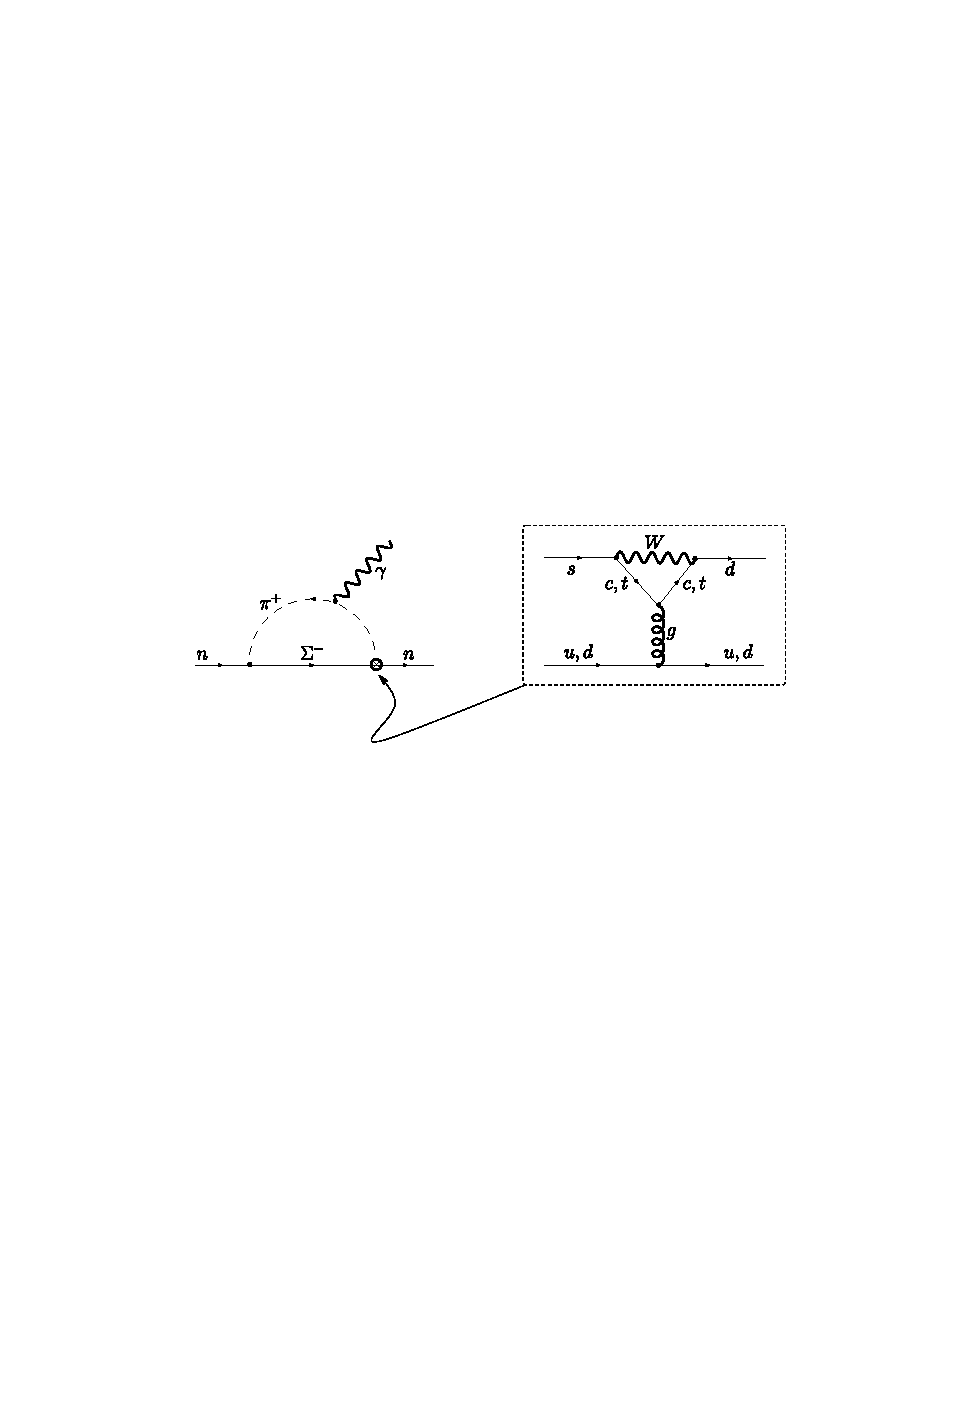
\includegraphics[width=0.6\textwidth]{figures/Pospelov_strong_penguin.pdf}
    \caption[The strong penguin diagram, the largest $CP$ violating phase contribution to the nEDM in the SM]
    {The strong penguin diagram (crossed vertex), the largest $CP$ violating phase contribution to the nEDM in the SM. Image from \cite{POS05}}
    \label{fig:strong_penguin}
\end{figure}

There are two sources of $CP$ violation in the Standard Model (\acrshort*{sm}). The first is found in the electroweak sector, via the Cabbibo-Kobayashi-Maskawa (CKM) matrix \cite{ckm1973, ChauKeung1984, pdg2022}.
%
\begin{align}
    V_\text{CKM} &= \left( \begin{matrix}
    V_\text{ud} & V_\text{us} & V_\text{ub} \\
    V_\text{cd} & V_\text{cs} & V_\text{cb} \\
    V_\text{td} & V_\text{ts} & V_\text{tb} \\
    \end{matrix} \right) \label{eq:CKM} \\
    &= \left( \begin{matrix}
    c_{12}c_{13} & s_{12}c_{13} & s_{13}e^{-i\delta} \\
    -s_{12}c_{23}-c_{12}s_{23}s_{13}e^{i\delta} & c_{12}c_{23}-s_{12}s_{23}s_{13}e^{i\delta} & s_{23}c_{13} \\
    s_{12}s_{23}-c_{12}c_{23}s_{13}e^{i\delta} & -c_{12}s_{23}s_{13}e^{i\delta} & c_{23}c_{13} \\
    \end{matrix} \right)
\end{align}
%
where $c_{ij}=\cos\theta_{ij}$, $s_{ij}=\sin\theta_{ij}$, and $\delta\approx1.2\text{ rad}$ is the $CP$ violating phase.

$V_\text{CKM}$ is unitary $(V_\text{CKM}V_\text{CKM}^\dag=I)$. For a $3 \times 3$ unitary matrix, the nine unknown complex elements of $V_{ij}$ may be reduced to three real numbers (rotation angle $\theta_{ij}$) and one phase ($\delta$), where the phase accounts for $CP$ violation.

We now examine contributions to the nEDM in the SM, beginning with quark EDMs. The neutron is a composite object consisting of three valence quarks ($udd$) and a sea of gluons and mesons. At tree level, there is no diagram generating an EDM interaction of one quark of the neutron with an electric field. At one loop, each CKM matrix element comes with a complex conjugate, thus negating any $CP$ violating phase. At the two loop level, the sum over all quark flavors in intermediate states leads to a vanishing EDM \cite{schmidt-wellenburg_quest_2017, czarnecki2018}.

In fact, the quark EDM appears only starting at the three loop level, with the largest effect from the exchange of two W bosons and one gluon. Taking a simplified valence approach to estimating the nEDM gives \cite{czarnecki2018}
%
\begin{gather}
    \gls*{d_n}^\text{valence} = \frac{4}{3}d_d - \frac{1}{3}d_u \lesssim 10^{-34}\,e\text{ cm}
\end{gather}

The largest $CP$ violating phase contribution to the nEDM arises from the so-called strong penguin diagram (Fig.~\ref{fig:strong_penguin}) \cite{POS05}. The contribution to a nEDM is enhanced by a long distance $\pi^-$ loop, and it is estimated to be
%
\begin{gather}
    \gls*{d_n}^\text{penguin} \sim 10^{-32}\,e\text{ cm}
\end{gather}
%
This is significantly lower than current experimental limits on the nEDM ($\sim 10^{-26}\,e\text{ cm}$ \cite{ABE20}). Further improvements to nEDM measurements are effective probes of beyond Standard Model (\acrshort*{bsm}) physics.

%%%%%%%%%%%%%%%%%%%%%%%%%%%%%%%%%%%%%%%%%

\subsection{Strong CP problem}

%%%%%%%%%%%%%%%%%%%%%%%%%%%%%%%%%%%%%%%%%

The second source of $CP$ violation in the SM comes from the quantum chromodynamics (QCD) Lagrangian term for the strong interaction. The $CP$ violating dimension 4 operator is
%
\begin{gather}
    \mathcal{L}_\text{QCD}^\text{CP\textendash odd}=\frac{g^2_s}{32\pi^2}\bar{\theta}G^a_{\mu\nu}\tilde{G}^{\mu\nu, a}
\end{gather}
%
where $g_s$ is the strong interaction coupling, $\bar{\theta}$ is the $CP$ violating phase, and $G^a_{\mu\nu}$ is the QCD gluon field tensor. It provides an nEDM contribution on the order of \cite{cp_violation_wo_strangeness}
%
\begin{gather}
    \gls*{d_n}^\text{QCD}\sim \bar{\theta}\times 10^{-16}\,e\text{ cm}
\end{gather}
%
Current experimental limits imply that $\bar{\theta}\lesssim 10^{-10}$, an arbitrarily tiny number given that the phase $\bar{\theta}$ has a permissible range $[0, 2\pi]$. There is no inherent reasoning as to why $\bar{\theta}$ is so small, resulting in the ``strong $CP$ problem.''

One proposed solution to the strong $CP$ problem is the axion \cite{peccei_quinn_axion}, a dark matter candidate. See Refs.~\cite{BAER20151, kim_gianpaolo_2010} for reviews on the topic.

%%%%%%%%%%%%%%%%%%%%%%%%%%%%%%%%%%%%%%%%%

\section{Baryon asymmetry of the universe}

%%%%%%%%%%%%%%%%%%%%%%%%%%%%%%%%%%%%%%%%%

The $CPT$ theorem implies that for any particle there should be an antiparticle of equal mass, decay width, and opposite charge. Particles and antiparticles should have equal distributions at thermal equilibrium. By these symmetry arguments, one would reasonably expect that the universe should contain equal amounts of particles and antiparticles, or that particles and antiparticles mostly annihilated during the early universe and are now very sparse.

In reality, this is not the case. Estimates of the expected baryon matter/anti-matter asymmetry in the universe (\acrshort*{bau}) is 8 orders of magnitude smaller than what is observed using the cosmic microwave background (CMB) \cite{Mor13, Dubbers2011}.

Sakharov \cite{Sakharov_1991} first suggested 3 conditions for baryogenesis, the production of BAU from an initally symmetric state in the early universe. The Sakharov criteria are:
%
\begin{enumerate}
    \item Baryon number violation: For some initial baryon number $B=0$ there must be some interaction that violates baryon number to proceed to a universe with $B>0$.
    \item $C$ and $CP$ violation: If $C$ and $CP$ are exact symmetries, then the probability of converting matter to antimatter is the same as the reverse process, resulting in $B=0$.
    \item Breaking of thermal equilibrium:  At thermal equilibrium, there is no preferred direction for time and $CPT$ invariance prevents baryon excess, negating the effect of any $CP$ violating processes.
\end{enumerate}

In the SM, there is an insufficient departure from thermal equilibrium and too little $CP$ violation for baryogenesis to be permitted. Reference~\cite{Dubbers2011} describes this in further detail.

%%%%%%%%%%%%%%%%%%%%%%%%%%%%%%%%%%%%%%%%%

\section{Beyond standard model physics}

%%%%%%%%%%%%%%%%%%%%%%%%%%%%%%%%%%%%%%%%%

\begin{figure}
    \centering
    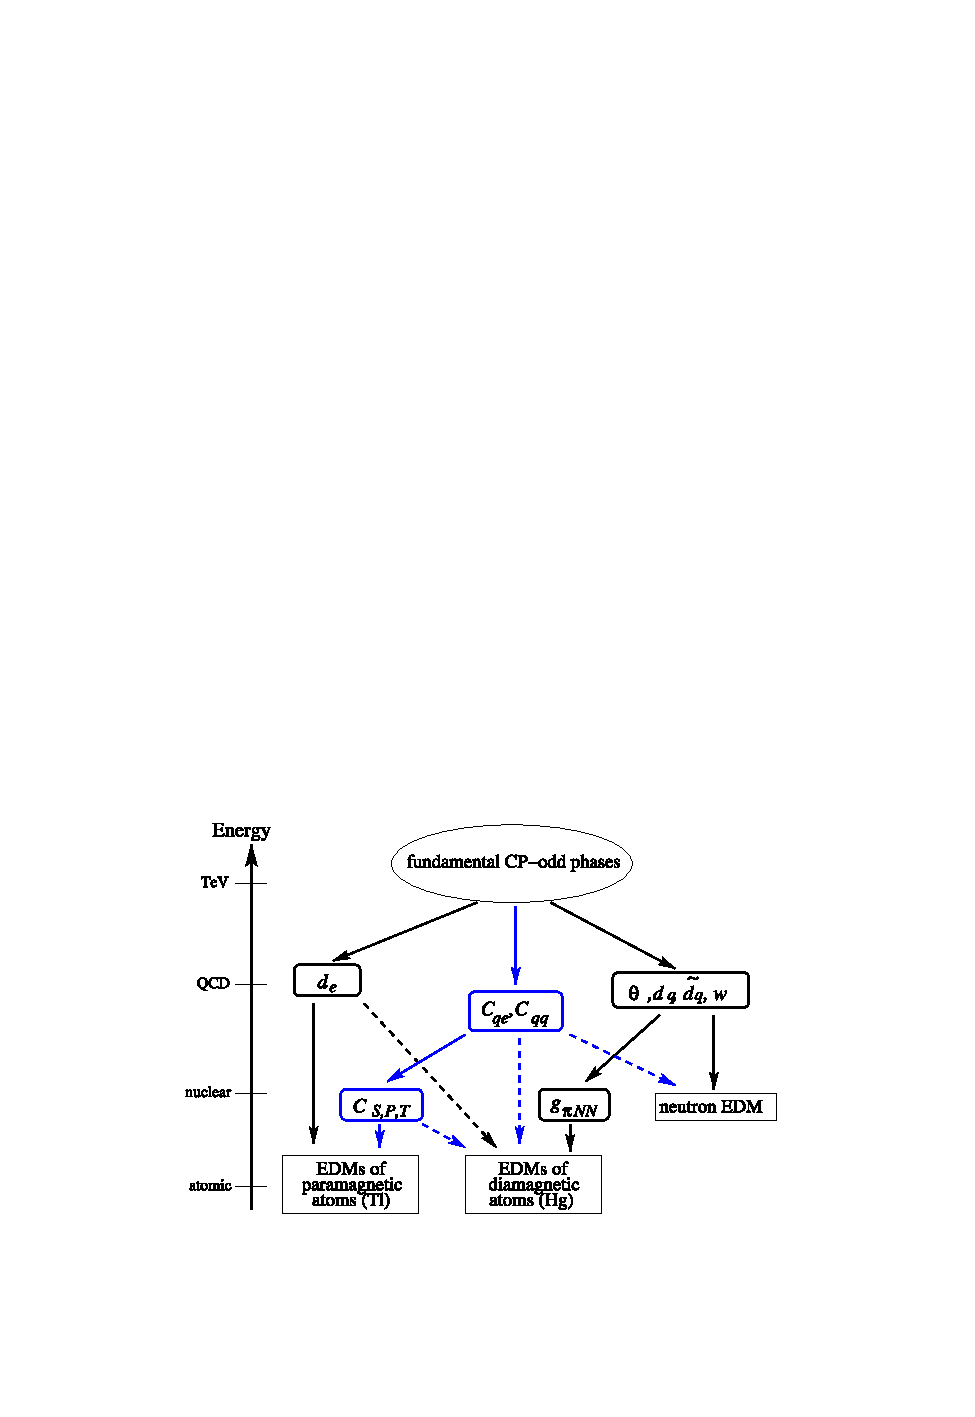
\includegraphics[width=0.75 \textwidth]{figures/Pospelov_BSM_CPV.pdf}
    \caption[A hierarchy of scales between BSM $CP$ violating sources and 3 general types of EDM observables.]
    {A hierarchy of scales between BSM $CP$ violating sources and 3 general types of EDM observables. Dashed lines depict weaker dependencies. Image from Ref. \cite{POS05}.}
    \label{fig:bsm_cp_violation}
\end{figure}

Physics beyond the SM (\acrshort{bsm}) is required for additional sources of $CP$ violation. For nEDM and EDM experiments, $CP$ violating contributions from the SM are effectively background, making EDMs very sensitive tests of BSM physics. Most SM extensions treat the SM as the low energy limit of a higher framework. $CP$\textendash odd parameters propagate from a $\sim$\unit{\tera\eV} scale down to a low energy observable (Fig.~\ref{fig:bsm_cp_violation}). Unfortunately, extracting a $CP$ violating phase from such an observable becomes difficult, requiring cross references of multiple EDM measurements. For reviews on new sources of $CP$ violation see Refs.~\cite{Cir10, POS05, ENG13, CHU19}.

%%%%%%%%%%%%%%%%%%%%%%%%%%%%%%%%%%%%%%%%%

\section{A brief history of nEDM experiments}\label{sec:history_nedm}

%%%%%%%%%%%%%%%%%%%%%%%%%%%%%%%%%%%%%%%%%

\begin{figure}
    \centering
    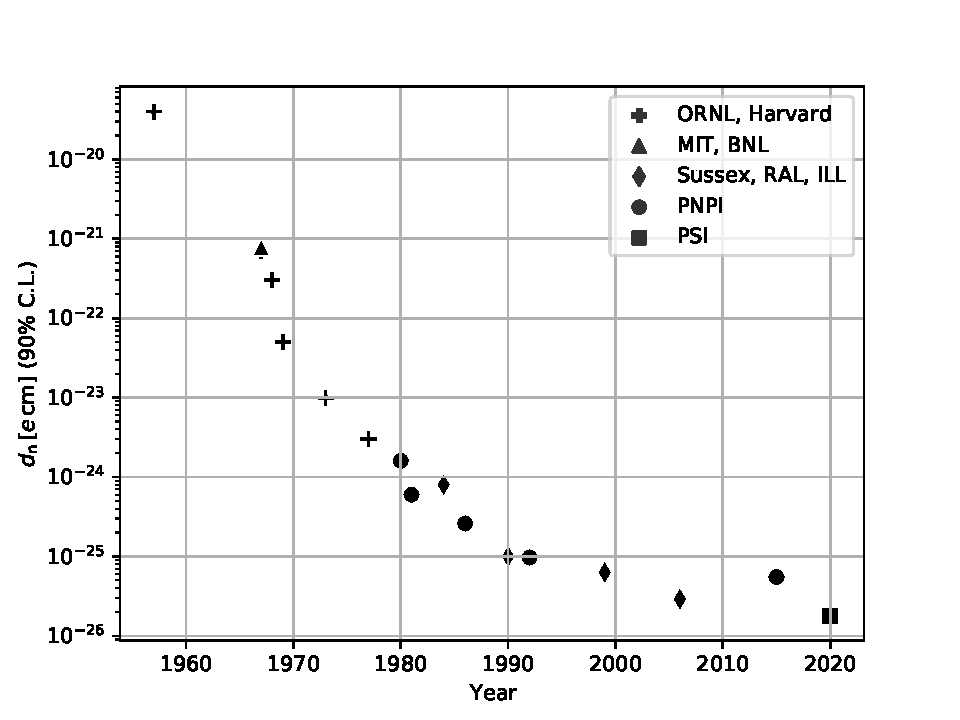
\includegraphics[width=0.85 \textwidth]{figures/nEDM-history.pdf}
    \caption[History of published nEDM measurements and the institutions involved.]{History of published nEDM measurements and the institutions involved. See Refs.~\cite{ramsey_nedm_1950, ramsey_nedm_1957, miller_nedm_1967, shull_nedm_1967, dress_nedm_1968, cohen_nedm_1969, dress_nedm_1973, dress_nedm_1977, altarev_nedm_1980, altarev_nedm_1981, pendlebury_nedm_1984,
    altarev_nedm_1986, smith_nedm_1990, altarev_nedm_1992, altarev_nedm_1996, harris_nedm_1999, BAK06, ABE20, pnpi_nedm_2015}. The vertical dotted line refers to the measurement of $CP$ violation in $K^0$ decay~\cite{christenson_1964}.}
    \label{fig:nEDM-history}
\end{figure}

The first nEDM experiment was begun by Ramsey in 1950, with the first result published in 1957 \cite{ramsey_nedm_1950, ramsey_nedm_1957}. The upper bound on $\gls*{d_n}$ has decreased steadily ever since (Fig.~\ref{fig:nEDM-history}). Early nEDM measurements \cite{miller_nedm_1967, baird_nedm_1969, cohen_nedm_1969, dress_nedm_1977} used thermal neutrons (\num{10000} to \qty{50000}{\micro \eV}) passing a meter-scale apparatus. The sensitivity of beam nEDM measurements was primarily limited by a $\vv{v}\times\vv{E}$ systematic effect (Sec.~\ref{sec:v_cross_E}).

By 1980, nEDM experiments \cite{altarev_nedm_1980, altarev_nedm_1981} used ultracold neutrons (\ucn), which have kinetic energies $\leq \qty{300}{\nano\eV}$. This enabled measurements with neutrons stored in material bottles \cite{smith_nedm_1990}. See Chap.~\ref{chap:UCN} for \ucn properties. Lower \ucn velocities and a population-averaged velocity of almost zero mitigated $\vv{v}\times\vv{E}$ systematics. 

nEDM experiments continued to improve with increased densities of stored \ucn, advances in magnetic shielding, and more sensitive magnetometry. One significant innovation was the introduction of a cohabitating comagnetomer, a population of $\ce{^{199}Hg}$ atoms that occupied the same space as \ucn, for monitoring magnetic field drifts within the storage volume~\cite{BAK06}. 

Most nEDM experiments (including beam measurements) use the same measurement principle, the Ramsey method of oscillatory fields \cite{ramsey_molecular_1950}. This technique is described in Chap.~\ref{chap:spinManipulation}. 

The current upper limit on the nEDM has been set by an experiment performed at the Paul Scherrer Institute ($\gls*{d_n}\leq 1.8\times10^{-26}e\,\text{cm [90\% \acrshort{cl}]}$)~\cite{ABE20} and there are several efforts worldwide aimed at searching for the nEDM with improved sensitivity~\cite{Alarcon2022}. The nEDM experiment at \acrlong*{lanl} (\acrshort*{lanl}) will use the Ramsey method to search for the nEDM with an uncertainty goal of $\delta \gls*{d_n} = 2.7\times10^{-27}e\text{ cm (90\% \acrshort{cl})}$.


%%%%%%%%%%%%%%%%%%%%%%%%%%%%%%%%%%%%%%%%%

\chapter{Ultracold neutrons}\label{chap:UCN}

%%%%%%%%%%%%%%%%%%%%%%%%%%%%%%%%%%%%%%%%%

Ultracold neutron(s) (\ucn) are neutrons of very low kinetic energy ($\lesssim \qty{300}{\nano\eV}$) that have a number of convenient properties useful in experiments involving fundamental physics. Modern nEDM experiments are performed almost exclusively using UCN \cite{BAK06, SER15, ABE20} (an alternative is proposed in Ref.~\cite{PIE13}). Depending on the optical potential (Sec.~\ref{sec:ucn_matter_int}), \ucn may be contained at all angles of incidence by material bottles. They are also of low enough energies that they may be influenced by gravitational and magnetic potentials (Sec.~\ref{sec:ucn_grav_em}). Due to the ease of manipulation and transport, \ucn can be moved away from the production source, where backgrounds are typically high, into shielded environments where backgrounds may be controlled. \ucn are easy to polarize, and their polarization is easily measured (Sec.~\ref{sec:ucn_polarizers}). Neutrons are also abundantly available (albeit bound in nuclei) and when freed have a long lifetime (Sec.~\ref{sec:weak_interaction}).

%%%%%%%%%%%%%%%%%%%%%%%%%%%%%%%%%%%%%%%%%

\section{UCN properties}

%%%%%%%%%%%%%%%%%%%%%%%%%%%%%%%%%%%%%%%%%

A population of \ucn may be treated as an ideal gas with a few unique characteristics \cite{golubUCN}: 
%
\begin{itemize}
    \item \ucn wall collisions are mostly elastic and specular. Inelastic scattering results in a neutron being upscattered (heated) from the \ucn energy range and lost. \ucn gas in a container is in a pseudo equilibrium where the gas velocity is isotropic in the storage volume
    \item UCN\textendash UCN collisions are negligible, and the mean free path of a \ucn is characterized by the geometry of the storage volume
    \item Due to gravity, \ucn density tends to decrease as height increases within the storage volume.
    \item \ucn gas density decreases over time as \ucn are lost to $\beta$ decay and wall collisions.
\end{itemize}
%
\ucn flow in guide tubes is similar to rarified gas flow in tubes, with the same caveats described above.

%%%%%%%%%%%%%%%%%%%%%%%%%%%%%%%%%%%%%%%%%

\section{Gravitational and electromagnetic interactions}\label{sec:ucn_grav_em}

%%%%%%%%%%%%%%%%%%%%%%%%%%%%%%%%%%%%%%%%%

\ucn are of sufficiently low energy such that the influence of gravity is non-negligible. For gravitational acceleration $g_0$ acting on a neutron mass \gls{m_n}, the potential energy of at a height $h$ is given by
%
\begin{gather}
    V_g = \gls{mg}h
\end{gather}
%
where $\gls*{mg}=$\glsvalue*{mg} \cite{codata_2018}.

The magnetic moment of the neutron also interacts with a magnetic field \gls*{bField}, with the potential energy defined by
%
\begin{gather}
    V_B = - \vv{\gls{mu_n}}\cdot \gls*{bField}
\end{gather}
%
where $\gls*{mu_n}=60.307\,739(15)\text{ neV T}^{-1}$~\cite{codata_2018}. Spin dependent interactions in a magnetic field are further described in Chap.~\ref{chap:spinManipulation}.

The neutron charge limit is effectively zero~\cite{baumann_neutron_charge}
%
\begin{gather}
    \gls*{q_n}=\glsvalue*{q_n}\quad(68 \% \text{ c.l.})
\end{gather}

%%%%%%%%%%%%%%%%%%%%%%%%%%%%%%%%%%%%%%%%%

\section{Weak interaction}\label{sec:weak_interaction}

%%%%%%%%%%%%%%%%%%%%%%%%%%%%%%%%%%%%%%%%%

\begin{figure}[htp]
    \centering
    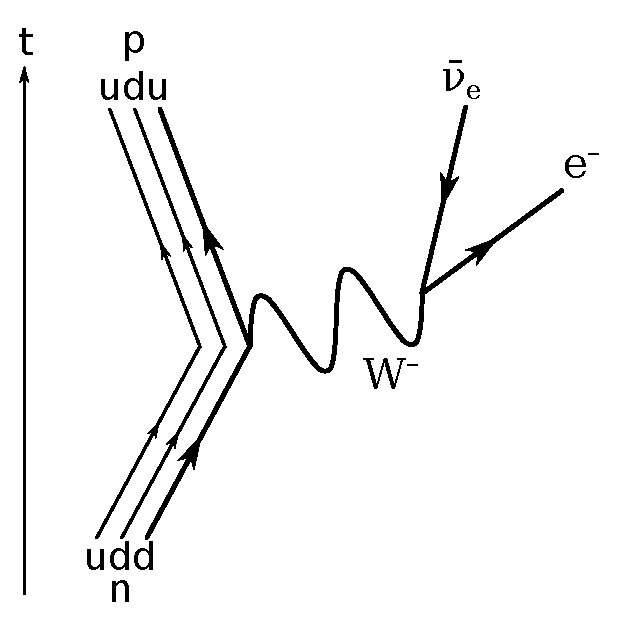
\includegraphics[width=0.3 \textwidth]{figures/beta_negative_decay.pdf}
    \caption[The leading order Feynman diagram of free neutron $\beta$ decay]
    {The leading order  Feynman diagram of free neutron $\beta$ decay. Image from \cite{beta_decay_fig}}
    \label{fig:beta_decay}
\end{figure}

Free neutrons undergo $\beta$ decay
%
\begin{gather}
    \text{n}\rightarrow \text{p}+ e^-+\bar{\nu}_e
\end{gather}
%
governed by the neutron lifetime (decay time) $\gls{tau_n}=\glsvalue*{tau_n}$ \cite{pdg2022}. The Feynman diagram to leading order for this process is given in Fig.~\ref{fig:beta_decay}. The neutron lifetime designates the amount of helium created during Big Bang nucleosynthesis. The CKM matrix element $V_\text{ud}$ (Eq.~\ref{eq:CKM}) can be determined from measurements of \gls{tau_n} in combination with measurements of $0^+\rightarrow0^+$ decays~\cite{Young2014}.

The most accurate neutron lifetime experiments to date have been storage experiments with \ucn held by magnetic and gravitational potentials, such as the UCN$\tau$ experiment at \acrshort{lanl} \cite{gonzalez_ucn_tau}. There is an ongoing disagreement between neutron lifetime storage experiments that count surviving \ucn and neutron lifetime cold beam experiments that count the proton decay products~\cite{czarnecki2018}.

The neutron beta decay directional distribution and total decay rate can be very generally written in terms of the neutron spin and lepton momenta by the expression~\cite{Young2014}
%
\begin{align}
    d\Gamma(\vv{p}_e, \vv{p}_{\bar{\nu}}) &= dE_e\,d\Omega_e \,d\Omega_{\bar{\nu}} \frac{F(E_e)\,p_e E_e (E_o-E_e)^2}{(2\pi)^5} \xi \nonumber \\
    &\quad\quad \times \left[1 + a\frac{\vv{p}_e \cdot \vv{p}_{\bar{\nu}}}{E_e E_{\bar{\nu}}}
    +b\frac{m_e}{E_e} + \langle \vv{S}_\text{n} \rangle \cdot
    \left( A\frac{\vv{p}_e}{E_e} + B \frac{\vv{p}_{\bar{\nu}}}{E_e} + D\frac{\vv{p}_e\times \vv{p}_{\bar{\nu}}}{E_e E_{\bar{\nu}}}
    \right) \right]
\end{align}
%
$\vv{S}_\text{n}$ is neutron spin, $F(E_e)$ is the Fermi function for final state interactions, $E_o$ is the endpoint energy, $E_e$ and $\vv{p}_e$ are electron energy and momentum, and $E_{\bar{\nu}}$ and $\vv{p}_{\bar{\nu}}$ are anti-neutrino energy and momentum.

Of interest are correlation coefficients $a$, $b$, $A$, $B$, and $D$, which are experimental observables. Measurements of these coefficients are a probe of the V\textendash A structure of the \acrshort{sm}. 
%
\begin{itemize}
    \item Electron-antineutrino asymmetry $a$ is measured from the proton spectrum.
    \item Fierz interference coefficient $b$ is measured from the $\beta$ spectrum. $b$ is nominally $0$ in the \acrshort*{sm}.
    \item Beta asymmetry $A$ is determined from the angular correlation between the emitted electron and neutron polarization.
    \item Spin-antineutrino asymmetry $B$ is found via the angular correlation of the recoil proton and neutron polarization.
    \item Triple product $D$ arises from the triple correlation between electron momentum, proton momentum, and neutron spin. $D$ is also nominally $0$ in the \acrshort*{sm}.
\end{itemize}

Reference~\cite{Young2014} provides a review of the $\beta$ decay experimental program at \acrshort{lanl}. (In this section we followed conventional notation for $\beta$ decay observables, but variables $a$, $b$, $A$, $B$, and $D$ will be used to denote other parameters for the remainder of this dissertation.) 


%%%%%%%%%%%%%%%%%%%%%%%%%%%%%%%%%%%%%%%%%

\section{Strong interaction}

%%%%%%%%%%%%%%%%%%%%%%%%%%%%%%%%%%%%%%%%%

Neutrons and protons are bound in nuclei via the strong interaction. In the low energy limit the strong force between the proton and neutron can be approximated by attractive square-well potential of depth \qty{40}{\mega\eV} with radius $2\times10^{-5}\text{ m}$. A more accurate representation is the Fermi potential, a square well with rounded corners. This Fermi potential is not to be confused with the optical potential, also proposed by Fermi, described in Sec.~\ref{sec:ucn_matter_int}. The force between a neutron and a nucleus is also approximated by a square well with $r=r_0A_m^{1/3}$ for mass number $A_m$ and the constant $r_0=1.2\times10^{-15}\text{ m}$ \cite{golubUCN}.

Neutrons may be absorbed (captured) by nuclei. When absorbed, a $\gamma$ ray or charged particle ($[\text{n},\text{p}]$ or $[\text{n},\alpha]$) is released. Absorption cross sections are further discussed in Sec.~\ref{sec:ucn_absorption}.

%%%%%%%%%%%%%%%%%%%%%%%%%%%%%%%%%%%%%%%%%

\section{UCN interactions with matter}\label{sec:ucn_matter_int}

%%%%%%%%%%%%%%%%%%%%%%%%%%%%%%%%%%%%%%%%%

Chapter 2 of Ref.~\cite{golubUCN} provides a very thorough description of neutron interactions with matter. The interaction of \ucn with some material is given by a complex ``optical potential,'' or ``pseudo-potential,'' of the form
%
\begin{gather}
    U = V - iW = \frac{2\pi\hbar^2}{\gls{m_n}}\gls*{rho_N} b_\text{c}-i\frac{\hbar}{2}\gls*{rho_N} \sigma_{\text{t}} v \label{eq:optical_potential}
\end{gather}
%
where \gls{m_n} is the neutron mass, $v$ is the velocity of the neutron, $b_\text{c}$ is the coherent neutron scattering length of the material, $\sigma_{\text{t}}$ is the total loss cross section, and $\gls*{rho_N}$ is number density. Number density can be expressed in units~[\unit{\meter^{-3}}] by the relation $\gls*{rho_N}=\rho_\text{mat}N_A/w_\text{at}$, where $\rho_\text{mat}$ [\unit{\g\per\m^3}] is material density, $w_\text{at}$ [\unit{\g\per\mole}] is atomic weight, and $N_A$ [\unit{\mole^{-1}}] is Avogadro's number.

The real component of optical potential $V$ describes the critical neutron energy that may be confined by a material, and the imaginary part $W$ describes absorption and upscattering within the material. Table~\ref{tb:optical_potentials} lists the UCN optical potentials of commonly used materials in nEDM experiments.

\begin{table}
\centering
\caption[UCN optical potentials of selected UCN materials. V is the real component and W is the imaginary component]{\label{tb:optical_potentials}UCN optical potentials of selected materials. $V$ is the real component and $W$ is the imaginary component.}
\begin{tabular}{
    l
    l
    S[table-format = 3.1]
    S[exponent-mode = scientific, table-format = 2.3e1]
    c
}
\toprule
Material & Abbrv. & {V [\unit{\nano\eV}]} & {W [\unit{\nano\eV}]} & Ref.\\ 
\midrule
Aluminum & Al & 54.1 & 0.00281 & \cite{atchison_transmission_2009}\\
Copper & Cu & 168 & 0.0252 & \cite{golubUCN}\\
Diamond-like carbon & \acrshort{dlc} & 250 & 0.0875 & \cite{Atchison2006} \\
Deuterated polystyrene & \acrshort{dps} & 161 & 0.0483 & \cite{bodek_storage_2008} \\
$\ce{^{58}}\text{Nickel}$ & $\ce{^{58}Ni}$ & 335 & 0.0503 & \cite{golubUCN} \\
Nickel Molybdenum & \acrshort{nimo} & 221.5 & 0.027 & \cite{bondar_losses_2017}  \\
Nickel Phosphorus & \acrshort{nip} & 213 & 2.3e-2 & \cite{pattie_jr_evaluation_2017}  \\
Stainless Steel & \acrshort{ss} & 183 & 0.055 & \cite{akatsuka_characterization_2023} \\
Polytetrafluoroethylene & \acrshort{ptfe} & 123 & & \cite{golubUCN} \\
& {\small(Teflon)} \\
\bottomrule
\end{tabular}
\end{table}

%%%%%%%%%%%%%%%%%%%%%%%%%%%%%%%%%%%%%%%%%

\subsection{Reflection and transmission}\label{sec:ucn_reflection_transmission}

%%%%%%%%%%%%%%%%%%%%%%%%%%%%%%%%%%%%%%%%%

Consider a neutron traveling in a material of potential $V$, with kinetic energy $K$. Let the neutron be incident on a second material of potential $V'$ and imaginary potential $W$, with an energy component perpendicular to the surface of the second material $K_\perp$. The incident neutron may be treated as a propagating wave function $\psi = \exp (ikx)$ with wave vector $k=\sqrt{2\gls{m_n}K/\hbar^2}$.

Reflection probability $R$ arises from continuity requirements at the incidence boundary, and is given by~\cite{golubUCN, schreyer_thesis}
%
\begin{gather}
    R = \begin{cases}
        \left| \frac{\sqrt{K_\perp}-\sqrt{K_\perp - (V'-V)}}{\sqrt{K_\perp} + \sqrt{K_\perp - (V'-V)}}\right|^2 \quad \text{for } K_\perp > (V'-V) \\
        \left| \frac{\sqrt{K_\perp}-\sqrt{K_\perp - (V'-V) + iW}}{\sqrt{K_\perp} + \sqrt{K_\perp - (V'-V) + iW}} \right|^2 \quad \text{for } K_\perp < (V'-V) \label{eq:loss_on_reflection}
    \end{cases}
\end{gather}
%
Under the condition $K_\perp < (V'-V)$, the neutron cannot be transmitted, only reflected. However, as per Eq.~\ref{eq:loss_on_reflection}, there is a reflection loss probability. The wave function of a reflected \ucn penetrates a small distance into the incidence surface, where it may be lost by the interactions described in Sec.~\ref{sec:ucn_absorption}.

If $K_\perp > (V'-V)$ and the neutron is not reflected, it undergoes refraction and is transmitted through the surface into the second material. The energy of the neutron within the second material is given by $K'=K-(V'-V)$. The refraction is analogous to Snell's law, where the velocity component in the first material perpendicular to the refraction surface $v_\perp$ is changed and the component parallel to the surface $v_\parallel$ is unaltered. The velocity in the second material $v'$ is given by
%
\begin{align}
    \vv{v}' &= \vv{v}_\parallel+ \vv{v}'_\perp \\
    &= \vv{v}_\parallel + \left( \sqrt{\frac{K_\perp}{K_\perp - (V'-V)}} \right)\vv{v}_\perp \\
    &= \vv{v} + \left( \sqrt{\frac{K_\perp}{K_\perp - (V'-V)}} - 1 \right)\vv{v}_\perp
\end{align}

%%%%%%%%%%%%%%%%%%%%%%%%%%%%%%%%%%%%%%%%%

\subsection{Absorption and up-scattering}\label{sec:ucn_absorption}

%%%%%%%%%%%%%%%%%%%%%%%%%%%%%%%%%%%%%%%%%

The two main loss mechanisms for \ucn within a material are absorption and inelastic up-scattering. Absorption occurs when the neutron is captured by nuclei, and inelastic upscattering occurs when a thermally vibrating nucleus increases the energy of \ucn such that it may no longer be stored. The total loss cross section $\sigma_{\text{t}}$ (from Eq.~\ref{eq:optical_potential}) is the sum of absorption cross section $\sigma_\text{abs}$ and inelastic up-scattering cross section $\sigma_\text{inel}$.

Absorption cross sections are well quantified (see Ref.~\cite{nist_neutron_cross_sections}), but up-scattering cross sections are mostly unknown. Among many other factors, surface impurities with large inelastic scattering cross sections (e.g. hydrogen, $\sigma_\text{inel} \sim \qty{80}{\barn}$ \cite{nist_neutron_cross_sections}), will heavily affect up-scattering probabilities. When simulating \ucn material interactions it is often easier to make the assumption $\sigma_{\text{t}} \cong \sigma_\text{abs}$, and to treat up-scattering as a separate effective loss per bounce parameter, as described in Sec.~\ref{sec:loss_per_bounce}.

The absorption cross section $\sigma_\text{abs}$ is proportional to $1/v$. From the second term of Eq.~(\ref{eq:optical_potential}) it becomes apparent that $W$ is independent of neutron velocity in the material.

Absorption loss probability may be expressed by non-conservation of current density $\vv{j}$ \cite{golubUCN}
%
\begin{gather}
    \vv{j} = \frac{\hbar}{2m} ( \psi^* \vv{\nabla} \psi - \psi \vv{\nabla}\psi^*)
\end{gather}
%
For some neutron wave function propagating through a material $\psi = \exp (ik'x)$ with wave vector $k'=\sqrt{2m(K'+iW)}/\hbar$. This gives
%
\begin{gather}
    j \propto e^{-2\,\text{Im}(k')x}
\end{gather}
%
The loss probability after traveling is distance $x$ through a material is then
%
\begin{gather}
    P_\text{abs}= 1 - \exp \left[2\,\text{Im}\left( \frac{\sqrt{2m(K'+iW)}}{\hbar}\right)x \right]\label{eq:pentrack_absorption}
\end{gather}
%
Equation~\ref{eq:pentrack_absorption} is the absorption probability calculation utilized in the \ucn simulation software \pentrack~\cite{schreyer_pentrack} (see Chap.~\ref{chap:simulations}). Another equivalent method for quantifying neutron absorption within a material is discussed in Sec.~\ref{sec:beer_lambert_law}.

%%%%%%%%%%%%%%%%%%%%%%%%%%%%%%%%%%%%%%%%%

\subsection{Loss per bounce}\label{sec:loss_per_bounce}

%%%%%%%%%%%%%%%%%%%%%%%%%%%%%%%%%%%%%%%%%

The average loss probability per bounce $\bar{\mu}(K)$ for a \ucn of kinetic energy $K$ is obtained by assuming ideal gas conditions and averaging loss per bounce over all angles of incidence. Equation~(2.70) in Ref.~\cite{golubUCN} gives
%
\begin{gather}
    \bar{\mu} = 2f \left[ \frac{V}{K} \sin^{-1}\left( \frac{K}{V}\right)^{1/2} -\left( \frac{V}{K} - 1 \right)^{1/2} \right] \label{eq:lossPerBounce_golub}
\end{gather}
%
The loss factor is $f=W/V$, for optical potential terms $V$ and $W$ from Eq.~(\ref{eq:optical_potential}). For a more phenomenological treatment of loss per bounce, Eq.~(\ref{eq:lossPerBounce_golub}) may be modified by replacing $f$ with a free parameter $\mu$, a velocity independent effective loss per bounce. See Secs.~\ref{subsec:storageCurves} and \ref{sec:1D_random_walk} for example applications.

%%%%%%%%%%%%%%%%%%%%%%%%%%%%%%%%%%%%%%%%%

\subsection{Beer-Lambert Law}\label{sec:beer_lambert_law}

%%%%%%%%%%%%%%%%%%%%%%%%%%%%%%%%%%%%%%%%%

Neutron flux attenuation after passing through material can be described with the Beer-Lambert law. Here we model neutron absorption and elastic scattering within material.

Let a beam of neutrons be incident on a material with area $A$, thickness $dx$, and density of atoms (number density) $\gls*{rho_N}$. The number of atoms hit by the incident beam of intensity $I$ is given by $\gls*{rho_N} A\,dx$. The ``effective area'' of the atoms is given by $\sigma \gls*{rho_N} A \, dx$, where $\sigma$ is an absorption or scattering cross section of neutrons on the material.

Therefore, the probability of the a neutron being absorbed or scattered out of the beam in a material of thickness $dx$ is given by
%
\begin{gather}
    -\frac{dI}{I}=\frac{\sigma\gls*{rho_N} A}{A}dx
\end{gather}
%
where $dI$ is the change in intensity as the beam traverses the distance $dx$. Integrating both sides of the equation gives
%
\begin{align}
    \int^I_{I_0}\frac{dI}{I} &= -\int^x_0 \sigma \gls*{rho_N} \,dx \\
    \frac{I}{I_0} &= \exp(-\sigma \gls*{rho_N} x) \label{eq:beer_lambert_law_variant}
\end{align}
%
Where $I_0$ is the beam density intensity at the entrance of the material. Defining the mean free path inside the material as $\lambda_\text{mfp}=1/(\gls*{rho_N} \sigma)$ we get the Beer-Lambert law, which describes flux attenuation.
%
\begin{gather}
    I(x) = I_0 \exp(-x/\lambda_\text{mfp}) \label{eq:beer_lambert_law}
\end{gather}
%
 The Beer-Lambert law applies to neutrons, photons, and rarefied gases. See Appx.~\ref{appx:199hg_pumping} for an example application to the \qty{254}{\nano\meter} laser used for optical pumping of the $\ce{^199Hg}$ comagnetometer. 
 
 We consider the process of bulk elastic scattering, when the neutron collides with the material and has its trajectory altered according to a Lambertian distribution. The probability $P_\text{elastic}$ after traversing a distance $x$ through a material is given by
%
\begin{gather}
    P_\text{elastic}=1-\exp(-x \gls*{rho_N} \sigma_\text{inc})
\end{gather}
%
where $\sigma_\text{inc}$ is the incoherent cross section for thermal neutrons (see Ref.~\cite{nist_neutron_cross_sections}). Similarly, the chance for absorption in a material for a \ucn with velocity $v$ may be described by
%
\begin{gather}
    P_\text{abs}= 1-\exp(-x \gls*{rho_N} \sigma_\text{abs}v_\text{thermal}/v)
\end{gather}
%
where $\sigma_\text{abs}$ is the absorption cross section for thermal neutrons ($v_\text{thermal}=\qty{2200}{\meter\per \s}$) as listed in Ref.~\cite{nist_neutron_cross_sections}.

%%%%%%%%%%%%%%%%%%%%%%%%%%%%%%%%%%%%%%%%%

\subsection{Diffuse reflections}\label{sec:diffuse_reflections}

%%%%%%%%%%%%%%%%%%%%%%%%%%%%%%%%%%%%%%%%%

\begin{figure}
\centering
%subfigure width gets "multiplied" by includegraphics width
\begin{subfigure}{.5\textwidth} 
  \centering
  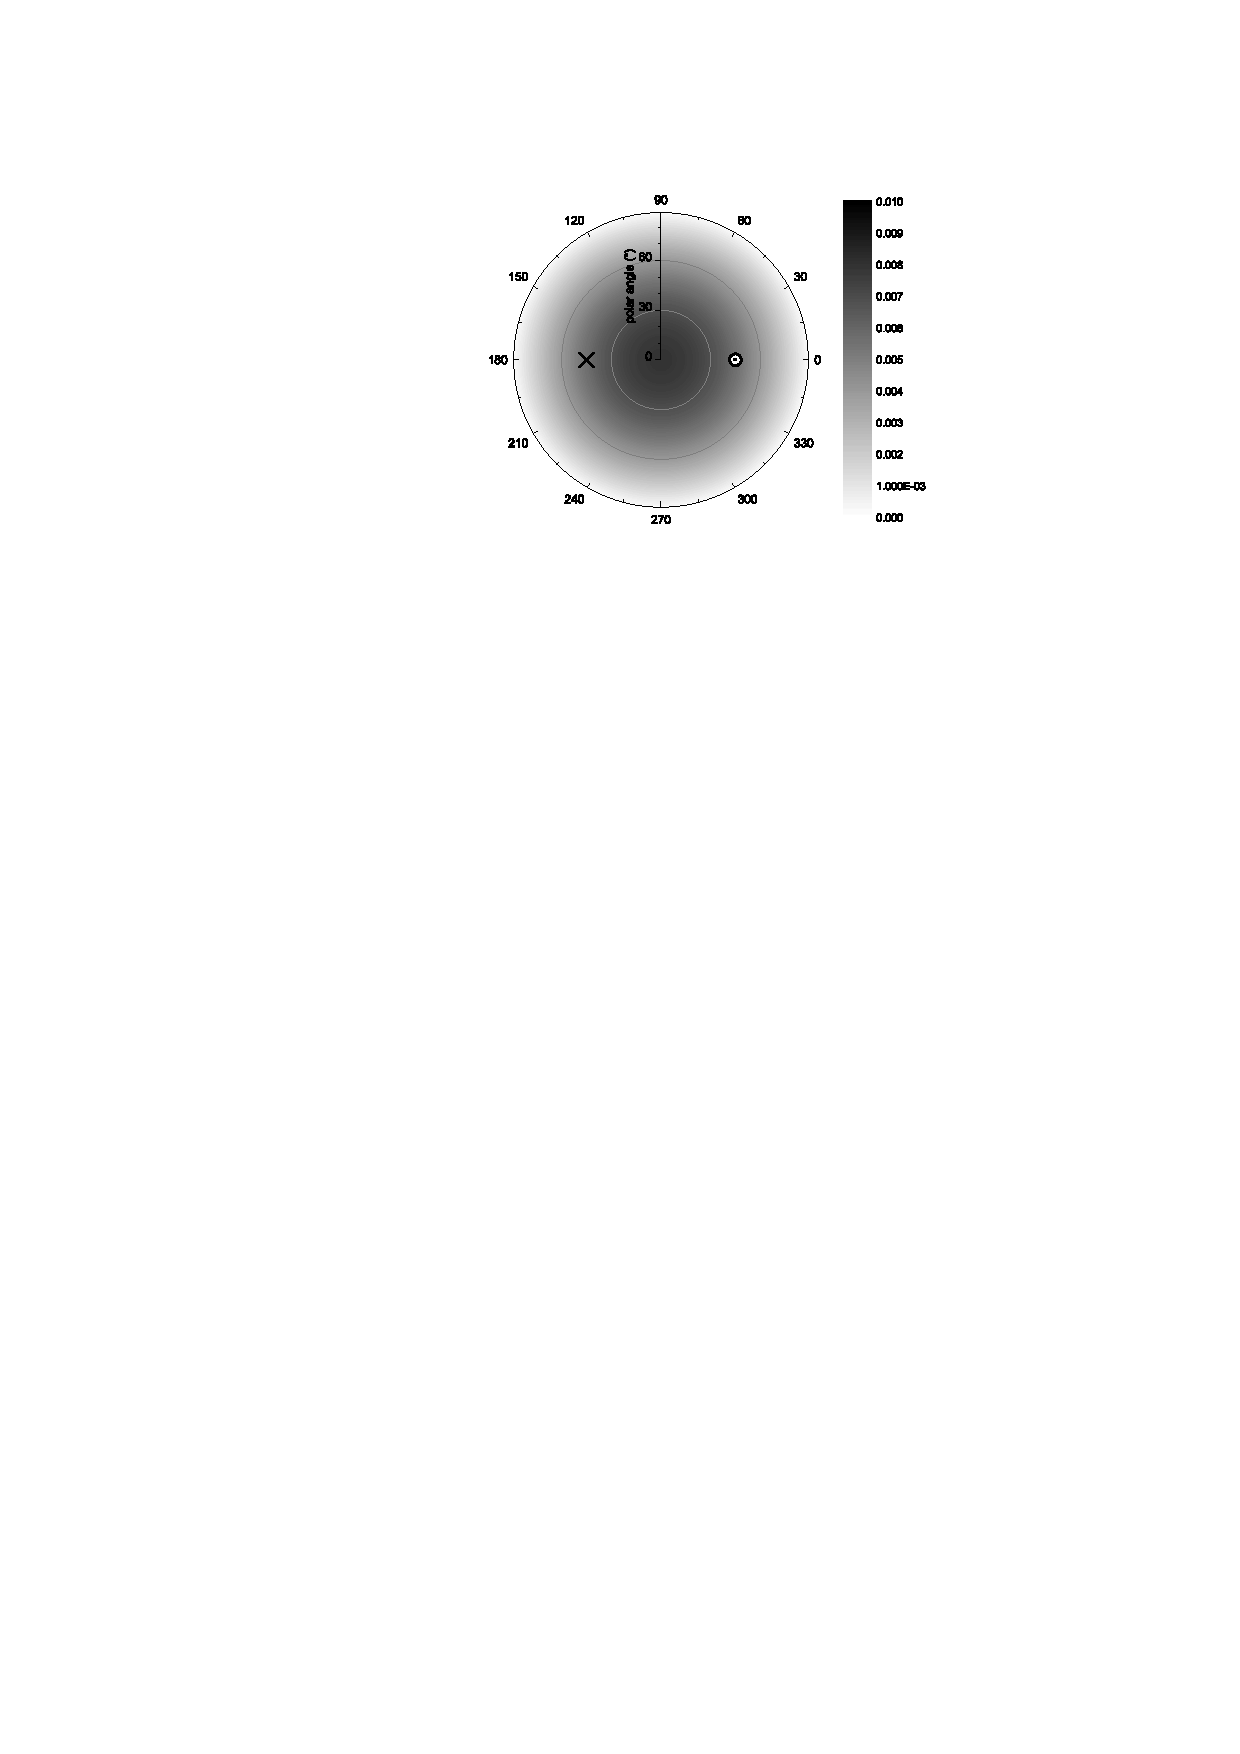
\includegraphics[width=\textwidth]{figures/schreyer_lambertian.pdf}
  \caption{Lambert ($\cos\theta$) distribution}\label{subfig:lambert_diffuse}
\end{subfigure}%DO NOT REMOVE THIS '%'
\begin{subfigure}{.5\textwidth}
  \centering
  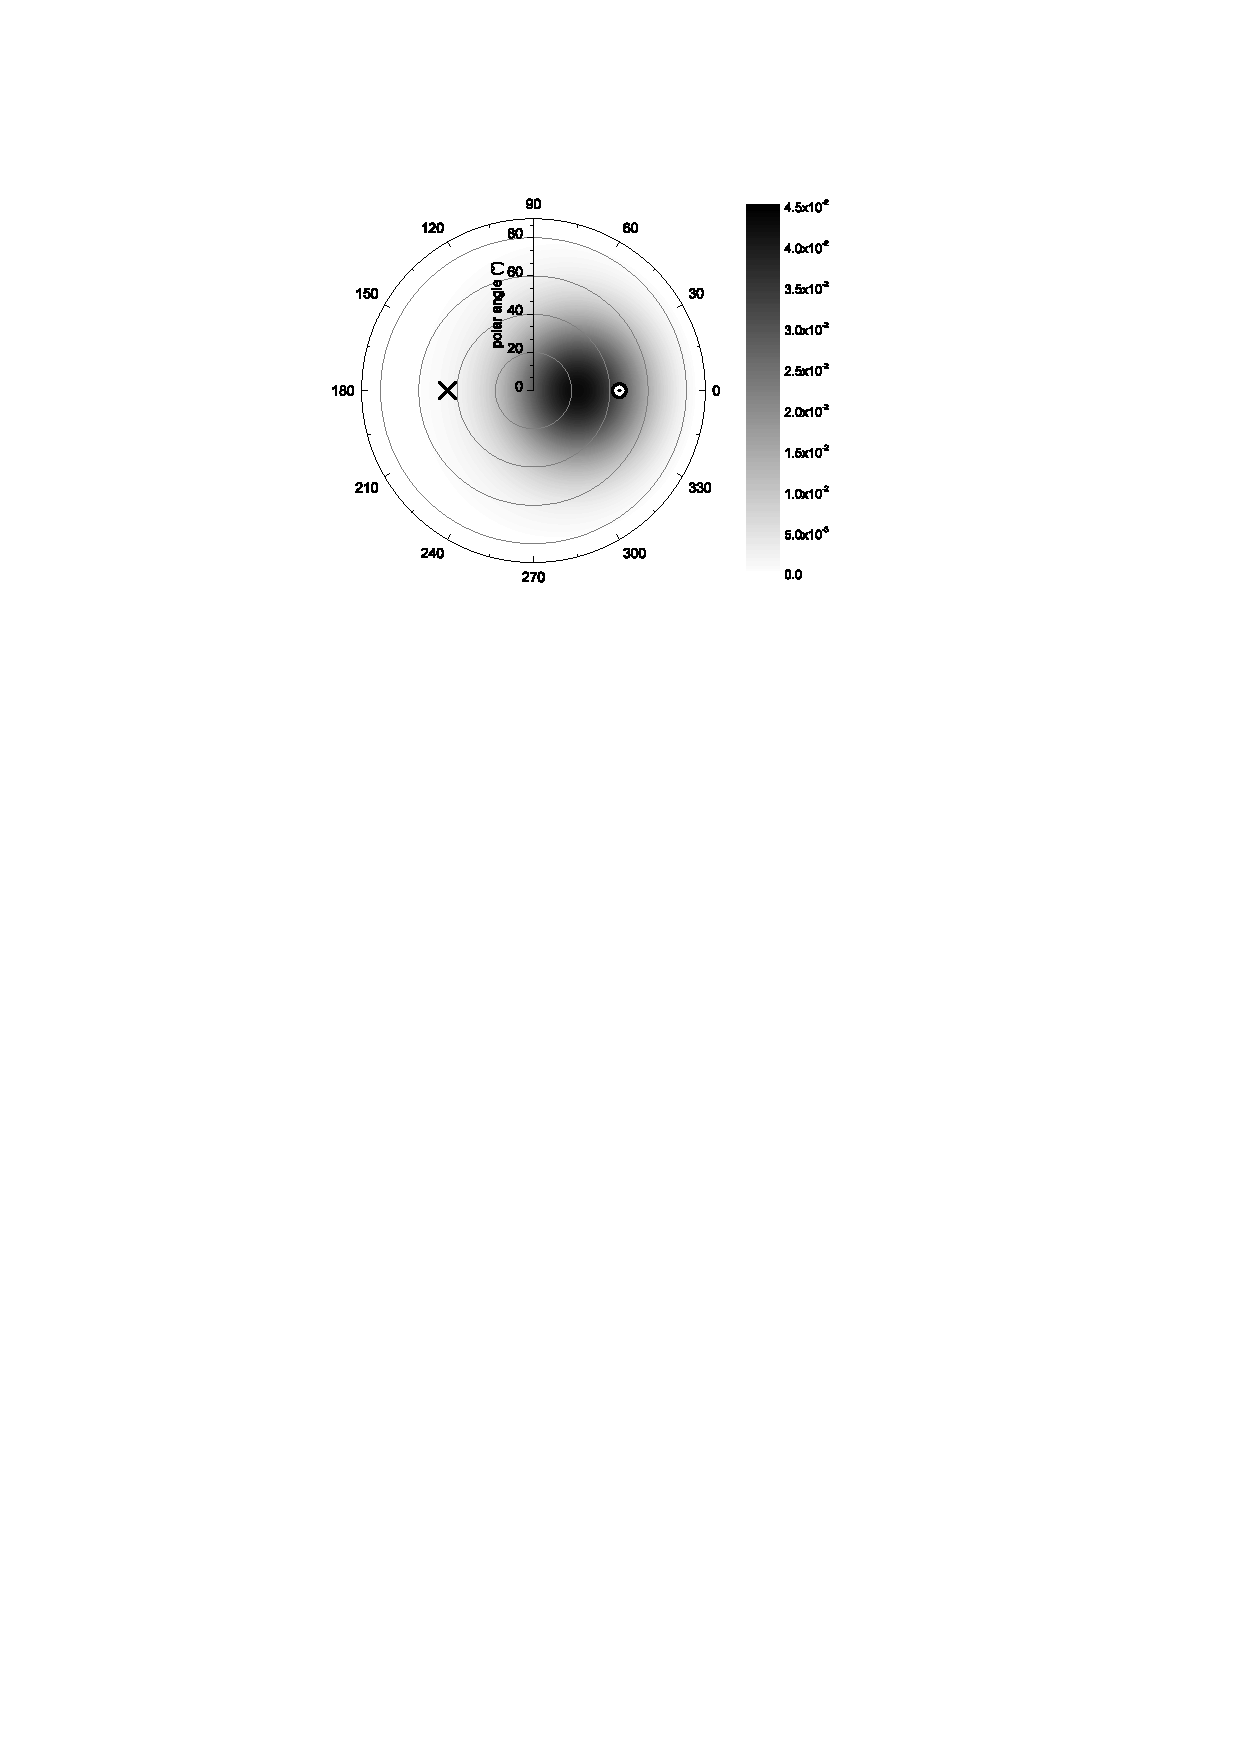
\includegraphics[width=\textwidth]{figures/schreyer_microroughness.pdf}
  \caption{Micro-roughness}\label{subfig:microroughness_diffuse}
\end{subfigure}
\caption[Two types of diffuse reflection]
{Two types of diffuse reflection. Images from Ref.~\cite{schreyer_thesis}. The cross is the incoming direction of the \ucn (\qty{45}{\degree}) and the dot is the direction of specular reflection. \textbf{(a)} Intensity of Lambertian reflection from Eq.~(\ref{eq:lambertian_reflection}) ($P_\text{L}=0.05$). \textbf{(b)} Intensity of micro-roughness reflection on \acrshort{ss} ($K=\qty{150}{\nano\eV}$, $V=\qty{183}{\nano\eV}$, $b_\text{MR}=\qty{2.5}{\nano\meter}$, $w_\text{MR}=\qty{20}{\nano\meter}$, $P_\text{MR}=\qty{4.9}{\percent}$)}
\label{fig:diffuse_reflection}
\end{figure}


\ucn incident on a smooth surface are usually reflected specularly, such that the angle of incidence is equal to the angle of reflection. However, there is a small material-dependent chance ($\sim\qtyrange{1}{10}{\percent}$) of diffuse (nonspecular) reflection. Diffusivity also affects the trajectory of refracted 
\ucn during transmission through a surface. The simplest version of diffuse reflection uses a Lambertian, or $\cos\theta$, distribution to determine the reflected intensity
%
\begin{gather}
    I_\text{L}(\theta)d\Omega=\frac{P_\text{L}}{\pi}\cos\theta\,d\Omega\label{eq:lambertian_reflection}
\end{gather}
%
where $P_\text{L}$ is some fixed probability of diffuse reflection and $d\Omega$ is the solid angle. The parameter $\theta$ has a range $[0,\pi/2]$. Lambertian reflection has no dependence on the angle of incidence (see Fig.~\ref{subfig:lambert_diffuse}).

A more accurate model of diffuse reflection is micro-roughness. A material surface is treated as a smooth plane with a perturbation, which causes diffuse scattering through diffraction and interference. Reference~\cite{atchison_diffuse_2010} experimentally validates the model described in Refs.~\cite{steyerl_1972, steyerl_surface_2010}, and an example of micro-roughness implementation in \ucn simulations is found in \pentrack~\cite{schreyer_pentrack}. Micro-roughness is characterized by surface roughness amplitude $b_\text{MR}$ and correlation length $w_\text{MR}$. For incident angle $\theta_\text{i}$ ($\phi_\text{i}=0$) and outgoing angles $\theta_\text{f}$, $\phi_\text{f}=0$, the reflection intensity $I_\text{R}$ and transmission intensity $I_\text{T}$ are given by~\cite{steyerl_1972, schreyer_thesis}
%
\begin{gather}
    \begin{align}
        I_\text{R}(k, \theta_\text{i}, \theta_\text{f}, \phi_\text{f})\,d\Omega_\text{f} &=  |S(\theta_\text{i})|^2|S(\theta_\text{f})|^2 F(k,\theta_\text{i}, \theta_\text{f}, \phi_\text{f})\,d\Omega_\text{f} \\
        I_\text{T}(k, k', \theta_\text{i}, \theta_\text{f}, \phi_\text{f})\,d\Omega_\text{f} &=  \frac{k'}{k}|S(\theta_\text{i})|^2|S(\theta_\text{f})|^2 F(k,\theta_\text{i}, \theta_\text{f}, \phi_\text{f})\,d\Omega_\text{f} \\
        S(\theta,k) &= \frac{2\cos\theta}{\cos\theta+\sqrt{\cos^2\theta-k_\text{c}/k}}
    \end{align}\\
    F(k,\theta_\text{i}, \theta_\text{f}, \phi_\text{f}) = \frac{k^4_\text{c}(b_\text{MR}w_\text{MR})^2}{8\pi\cos\theta_\text{i}} \exp \left[-\frac{(w_\text{MR}k)^2}{2} (\sin^2\theta_\text{i}+\sin^2\theta_\text{f} - 2\sin\theta_\text{i}\sin\theta_\text{f}\cos\phi_\text{f})\right]
\end{gather}
%
where following the notation from Sec.~\ref{sec:ucn_reflection_transmission}, the incident \ucn wave vector is $k=\sqrt{2\gls{m_n}K/\hbar^2}$, the transmitted wave vector is $k'=\sqrt{2\gls{m_n}(K - (V'-V))/\hbar^2}$, and the critical wave vector for total reflection is $k=\sqrt{2\gls{m_n}(V'-V)/\hbar^2}$.

Unlike Lambertian reflection, the probability of micro-roughness reflection or transmission is not a free parameter, and is given by
%
\begin{gather}
    P_\text{MR}=\int_{2\pi} I_\text{R,T}(k, \theta_\text{i}, \theta_\text{f}, \phi_\text{f})\,d\Omega_\text{i}=\int_0^{\pi/2}d\theta_\text{f}\int_0^{2\pi}d\phi_\text{f}\,I_\text{R,T}(k, \theta_\text{i}, \theta_\text{f}, \phi_\text{f})
\end{gather}
%
Fig.~\ref{subfig:microroughness_diffuse} shows an example of diffuse reflection using micro-roughness.
%%%%%%%%%%%%%%%%%%%%%%%%%%%%%%%%%%%%%%%%%

\chapter{UCN spin manipulation}\label{chap:spinManipulation}

%%%%%%%%%%%%%%%%%%%%%%%%%%%%%%%%%%%%%%%%%

Nuclear magnetic resonance (\acrshort*{nmr}) was first observed by Rabi in 1938 \cite{rabi_1938}, where he utilized a Stern-Gerlach experiment with a beam of nuclei traversing an inhomogenous magnetic field. He introduced an additional \acrshort{rf} magnetic field perpendicular to the static field. When the strength of the static field was tuned properly, there was a dip in beam intensity at the detector. This dip corresponded to a transition in the spin state of the nuclei, with the minimum at the resonance condition where the Larmor precession frequency of the nuclei in the static field matched the frequency of the \acrshort*{rf} field. Sweeping the strength of the static field to find the resonance enabled Rabi to measure the nuclear magnetic moment. Section~\ref{sec:rabi} describes the Rabi method in more detail, examining the more typical method where the static field is held constant and the \acrshort{rf} frequency is swept to find resonance.

In 1949, Ramsey \cite{ramsey_molecular_1950} improved upon Rabi's technique with what is now called the Ramsey method of separated oscillatory fields (Sec.~\ref{sec:ramsey-method}).  He divided the single oscillatory magnetic field at the center of the Rabi device into two shorter ones, one at the beginning of the beam and one at the end. This offers a number of advantages, the main one being that the peak near resonance is narrower than the peak from the Rabi method, giving higher resolution for determining the resonant frequency. The narrowing is analogous to the peaks in a double slit diffraction experiment, which are narrower than the peak from a single slit of equal width to the separation of the double slits~\cite{Ekspong1993}.

Of course, even the most advanced NMR techniques are useless if neutrons are inffectively polarized and if the polarization cannot be maintained. Section~\ref{sec:ucn_polarizers} discusses neutron polarization methodology, Sec.~\ref{sec:adiabaticity} introduces the adiabaticity parameter commonly used to characterize the conditions of neutron spin transport, and Sec.~\ref{sec:spin_relaxation} covers spin coherence.

%%%%%%%%%%%%%%%%%%%%%%%%%%%%%%%%%%%%%%%%%

\section{UCN polarizers}\label{sec:ucn_polarizers}

%%%%%%%%%%%%%%%%%%%%%%%%%%%%%%%%%%%%%%%%%

\begin{figure}
\centering
%subfigure width gets "multiplied" by includegraphics width
\begin{subfigure}{.5\textwidth} 
  \centering
  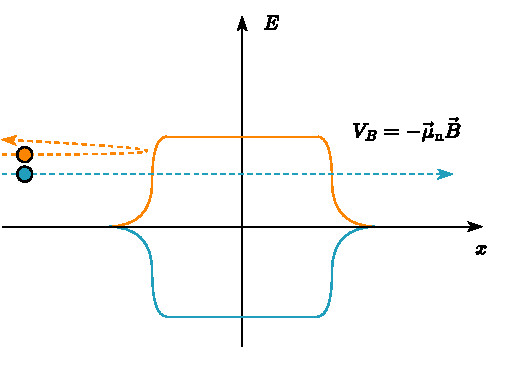
\includegraphics[width=\textwidth]{figures/ucn_polarization_1.pdf}
  \caption{Polarization with a strong magnetic field \newline potential $V_B$}\label{subfig:polarization_solenoid}
\end{subfigure}%DO NOT REMOVE THIS '%'
\begin{subfigure}{.5\textwidth}
  \centering
  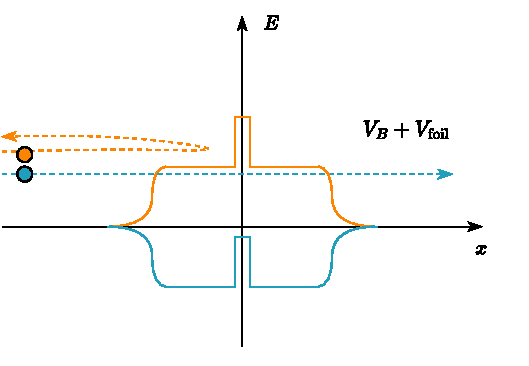
\includegraphics[width=\textwidth]{figures/ucn_polarization_2.pdf}
  \caption{Polarization using $V_B$ and thin \newline material ``foil'' with optical potential $V_\text{foil}$}\label{subfig:polarization_foil}
\end{subfigure}
\caption
{Two methods of UCN polarization. \legendbox{HFS-color} The lower line is the total potential experienced by a high field seeker. \legendbox{LFS-color} The upper line is the total potential experienced by a low field seeker.}
\label{fig:polarization_methods}
\end{figure}

From Sec.~\ref{sec:ucn_grav_em}, neutrons entering a magnetic region experience a potential, where the coupling of the neutron spin with the magnetic field determines the sign of the potential. High field seekers are defined as neutrons with $-\vv{\gls{mu_n}}\cdot\vv{B}<0$, and low field seekers are neutrons with $-\vv{\gls{mu_n}}\cdot\vv{B}>0$. The process of polarization passes high field seekers and rejects low field seekers in a population of \ucn.

There are two methods used in the LANL nEDM experiment for \ucn polarization: 
%
\begin{enumerate}
    \item A superconducting solenoid produces a high magnetic field ($\sim \qty{5}{\tesla}$), which polarizes neutrons coming from the \ucn source for use in the experiment. This system is described briefly in Sec.~\ref{sec:PM_description} and characterized in Chap.~\ref{chap:north_beamline_paper}.
    \item An analyzer (polarizer) is made of a thin Si or Al wafer upon which a layer of magnetic material is deposited. An external magnetic field ($\sim \qty{10}{mT}$) generated by ferromagnets saturates the magnetic layer. Refer to Sec.~\ref{sec:spin_flipper_analyzer} for details about the construction of the spin analyzer system.
\end{enumerate}
%
Figure~\ref{fig:polarization_methods} roughly illustrates the potentials seen by high field seekers and low field seekers in both polarization methods.


%%%%%%%%%%%%%%%%%%%%%%%%%%%%%%%%%%%%%%%%%

\section{Precession in a uniform static magnetic field\label{sec:larmor}}

%%%%%%%%%%%%%%%%%%%%%%%%%%%%%%%%%%%%%%%%%

We begin our examination of spin-dependent interactions with the classic undergraduate example of precession in a static field \cite{griffiths_quantum}. The Hamiltonian operator for a magnetic dipole moment in a magnetic field \gls*{bField} is
%
\begin{align}
    \hat{H}=-\hat{\mu}\cdot\gls*{bField}=-\gamma\hat{S}\cdot \gls*{bField}\label{eq:hamiltonian_operator}
\end{align}
%
for magnetic dipole moment operator $\hat{\mu}$, gyromagnetic ratio $\gamma$, and spin operator $\hat{S}=\frac{\hbar}{2}\vv{\sigma}$. Let \gls*{bField} be a static magnetic field such that $\gls*{bField}=B_0 \vv{z}$. Therefore,
%
\begin{gather}
    \hat{H}=-\gamma B_0 \hat{S}_z=-\frac{\gamma \hbar B_0}{2}\sigma_z\label{eq:larmor_1}
\end{gather}
%
The Pauli matrices, written as $\vv{\sigma}=(\sigma_x, \sigma_y, \sigma_z)$, are
%
\begin{gather}
    \sigma_{x}=\left(\begin{matrix}
    0 & 1\\
    1 & 0
    \end{matrix}\right)\quad
    \sigma_{y}=\left(\begin{matrix}
    0 & -i\\
    i & 0
    \end{matrix}\right)\quad
    \sigma_{z}=\left(\begin{matrix}
    1 & 0\\
    0 & -1
    \end{matrix}\right)
\end{gather}
%
The time dependent \schrodinger equation is
%
\begin{gather}
    i\hbar\frac{d}{dt}\Ket{\psi(t)}=\hat{H}\Ket{\psi(t)} \label{eq:schrodinger}
\end{gather}
%
where we write the spinor as 
\begin{gather}
    \Ket{\psi(t)}=\Ket{\begin{matrix}
        \psi_+(t)\\
        \psi_-(t)
    \end{matrix}}\label{eq:spinor}  
\end{gather}
%
Substituting (\ref{eq:larmor_1}) into (\ref{eq:schrodinger}),
\begin{gather}
    \left(\begin{matrix}
        \dot{\psi}_+\\
        \dot{\psi}_-
    \end{matrix}\right)
    = -\frac{i\omega_0}{2}
    \left(\begin{matrix}
        1 & 0\\
        0 & -1
    \end{matrix} \right)
    \left(\begin{matrix}
        \psi_+\\
        \psi_-
    \end{matrix}\right)\label{eq:larmor_2}
\end{gather}
where we define the Larmor precession frequency as
%
\begin{gather}
    \omega_0 = -\gamma B_0 \label{eq:larmor_freq}
\end{gather}
%
Eq.~(\ref{eq:larmor_2}) then simplifies into the differential equations
%
\begin{align}
    \dot{\psi}_+ &=\frac{-i\omega_0}{2}\psi_+ \label{eq:larmor_3}\\
    \dot{\psi}_- &=\frac{i\omega_0}{2}\psi_- \label{eq:larmor_4}
\end{align}
%
Let the initial condition at $t=0$ be 
$\Ket{\psi(t=0)}=\left( \begin{matrix}
    a_0 \\
    b_0
\end{matrix}\right)$. Solving Eqs.~(\ref{eq:larmor_3}) and (\ref{eq:larmor_4}) gives the solution
%
\begin{gather}
    \ket{\psi(t)}=\left(\begin{matrix}
        a_0e^{-i\omega_0 t/2} \\
        b_0e^{i\omega_0 t/2}
    \end{matrix}\right)\label{eq:larmor_solution}
\end{gather}
%
where $a_0$ and $b_0$ are complex numbers. To obtain the odds of measuring spin up along $x$, $y$, and $z$, we use the normalized eigenvectors of the Pauli matrices
%
\begin{gather}
    \Ket{S_z;+}=\left(\begin{matrix}
        1 \\
        0
    \end{matrix}\right),\quad
    \Ket{S_y;+}=\frac{1}{\sqrt{2}}\left(\begin{matrix}
        1 \\
        i
    \end{matrix}\right),\quad
    \Ket{S_x;+}=\frac{1}{\sqrt{2}}\left(\begin{matrix}
        1 \\
        1
    \end{matrix}\right)\label{eq:pauli_eigenvectors}
\end{gather}
%
Therefore,
%
\begin{align}
    \left| \Braket{S_z;+ | \psi(t)} \right|^2&= |a_0|^2 \\
    \left| \Braket{S_x;+ | \psi(t)} \right|^2&= \frac{1}{2} + \frac{1}{2}(a_0b_0^*+a_0^*b_0)\cos\,\omega_0t - \frac{1}{2}i(a_0b_0^*-a_0^*b_0)\sin\,\omega_0t \label{eq:larmor_5} \\
    \left| \Braket{S_y;+ | \psi(t)} \right|^2&= \frac{1}{2} + \frac{1}{2}i(a_0^*b_0-a_0b_0^*)\cos\,\omega_0t - \frac{1}{2}(a_0b_0^*+a_0^*b_0)\sin\,\omega_0t \label{eq:larmor_6}
\end{align}
%
This corresponds to the particle precessing about $\vv{z}$ at the Larmor frequency $\omega_0$. For an initial state $a_0=1/\sqrt{2}, b_0=1/\sqrt{2}$ (where the semiclassical spin vector points along $\vv{x}$ in the $x$--$y$ plane), Eqs.~(\ref{eq:larmor_5}) and (\ref{eq:larmor_6}) become
%
\begin{align}
    \left| \Braket{S_x;+ | \psi(t)} \right|^2&= \frac{1}{2} + \frac{1}{2}\cos\,\omega_0t \\
    \left| \Braket{S_y;+ | \psi(t)} \right|^2&= \frac{1}{2} - \frac{1}{2}\sin\,\omega_0t 
\end{align}

%%%%%%%%%%%%%%%%%%%%%%%%%%%%%%%%%%%%%%%%%

\section{Rabi resonance\label{sec:rabi}}

%%%%%%%%%%%%%%%%%%%%%%%%%%%%%%%%%%%%%%%%%

Following Ref.~\cite{may_thesis}, we now consider the case with a field $\vv{B_\text{c}}$ (which we will refer to as a ``circular \acrshort{rf}'') rotating at a frequency $\omega$ in the $x$--$y$ plane with an initial phase $\phi$ relative to $x$ in addition to the static field $\vv{B}_0$ considered in Sec.~\ref{sec:larmor}. The total field $\vv{B}$ is written as
%
\begin{gather}
    \vv{B}(t)=\vv{B_\text{c}}(t) + \vv{B_0}=B_\text{c}\left[ \cos (\omega t + \phi) \vv{x} + \sin (\omega t + \phi) \vv{y}\right] + B_0 \vv{z}\label{eq:B0_with_circular_rf}
\end{gather}
%
with the condition that $B_\text{c} \ll B_0$. The Hamiltonian operator from Eq.~(\ref{eq:hamiltonian_operator}) becomes
%
\begin{gather}
    \hat{H} = -\gamma \left( B_\text{c} \hat{S}_x \cos (\omega t + \phi) + B_\text{c} \hat{S}_y  \sin (\omega t + \phi) + B_0\hat{S}_z \right)\label{eq:rabi_hamiltonian}
\end{gather}
%
We define the resonant angular frequency for the circular \acrshort*{rf} as $\omega_\text{c}=-\gamma B_\text{c}$. Using the \schrodinger equation (\ref{eq:schrodinger}), this gives
%
\begin{gather}
    \left(\begin{matrix}
        \dot{\psi}_+\\
        \dot{\psi}_-
    \end{matrix}\right)
    = -\frac{i}{2}
    \left(\begin{matrix}
        \omega_0 & \omega_\text{c}e^{-i(\omega t + \phi)}\\
        \omega_\text{c}e^{i(\omega t + \phi)} & -\omega_0
    \end{matrix} \right)
    \left(\begin{matrix}
        \psi_+\\
        \psi_-
    \end{matrix}\right)\label{eq:rabi_1}
\end{gather}
%
where $\omega_0$ is the Larmor frequency (\ref{eq:larmor_freq}). We rewrite Eq.~(\ref{eq:rabi_1}) as
%
\begin{align}
    \dot{\psi}_+ &=\frac{-i}{2}\left( \omega_0 \psi_+ + \omega_\text{c} e^{-i(\omega t + \phi)} \psi_- \right)\label{eq:rabi_2}\\
    \dot{\psi}_- &=\frac{i}{2}\left( \omega_0 \psi_- - \omega_\text{c} e^{i(\omega t + \phi)} \psi_+ \right)\label{eq:rabi_3}
\end{align}
%
Equations~(\ref{eq:rabi_2}) and (\ref{eq:rabi_3}) may be solved numerically, as in Appx.~\ref{appx:ramsey_numerical}. To obtain an analytical solution, we make the change of variables $\psi_+ = \psi'_+ e^{-i(\omega t + \phi)/2}$ and $\psi_- = \psi'_- e^{i(\omega t + \phi)/2}$, which gives
%
\begin{align}
    \dot{\psi}'_+ &= \frac{i}{2}((\omega - \omega_0)\psi'_+ - \omega_\text{c} \psi'_-)\label{eq:rabi_4}  \\
    \dot{\psi}'_- &= -\frac{i}{2}(\omega_\text{c}\psi'_+ + (\omega - \omega_0) \psi'_-)\label{eq:rabi_5} 
\end{align}
%
We then decouple by taking another derivative of (\ref{eq:rabi_4}) and (\ref{eq:rabi_5}) with respect to $t$ and use some algebra to get
%
\begin{gather}
     \ddot{\psi'}_{\pm} = -\Omega^2 \psi'_{\pm}\label{eq:rabi_6}
\end{gather}
%
where we let the Rabi flopping frequency be 
%
\begin{gather}
   \Omega=\frac{\sqrt{(\omega - \omega_0)^2+\omega_\text{c}^2}} {2}  \label{eq:rabi_freq}
\end{gather}
%
The solution for (\ref{eq:rabi_6}) has the form
%
\begin{gather}
    \psi'_\pm= C_{\psi\pm}\cos\,\Omega t + D_{\psi\pm}\sin\,\Omega t
\end{gather}
%
which in the original basis is
%
\begin{gather}
    \psi_\pm= e^{\mp i (\omega t+\phi)/2}\left( C_{\psi\pm}\cos\,\Omega t + D_{\psi\pm}\sin\,\Omega t \right)
\end{gather}
%
Solving initial conditions (see Ref.~\cite{may_thesis}) for
$\Ket{\psi(t=0)}=\left( \begin{matrix}
    a_0 \\
    b_0
\end{matrix}\right)$, where $a_0$ and $b_0$ are complex, gives
%
\begin{align}
    \psi_+(t) &= e^{-i(\omega t + \phi)/2}\left(a_0 e^{i\phi/2} \cos \, \Omega t + D_{\psi +} \sin \, \Omega t\right) \\
    \psi_-(t) &= e^{i(\omega t + \phi)/2}\left(b_0 e^{-i\phi/2} \cos \, \Omega t + D_{\psi -} \sin \, \Omega t\right) \\
    D_{\psi +} &= \frac{i}{2\Omega}\left( a_0 e^{i\phi/2} (\omega - \omega_0) - \omega_\text{c}b_0 e^{-i\phi/2} \right) \\
    D_{\psi -} &= -\frac{i}{2\Omega} \left(a_0 \omega_\text{c}e^{i\phi/2} + b_0(\omega -\omega_0)e^{-i\phi/2} \right)
\end{align}
%
As before, the probability of measuring spin up along $x$, $y$, and $z$ are determined by using (\ref{eq:pauli_eigenvectors})
%
\begin{align}
    \left| \Braket{S_z;+ | \psi(t)} \right|^2&= \psi_+(t)\psi_+^*(t) \label{eq:rabi_circ_z} \\
    \left| \Braket{S_x;+ | \psi(t)} \right|^2&= \frac{1}{2} + \frac{1}{2}( \psi_+(t)\psi_-^*(t)) \label{eq:rabi_circ_x} \\
    \left| \Braket{S_y;+ | \psi(t)} \right|^2&= \frac{1}{2} + \frac{i}{2}( \psi_-(t)\psi_+^*(t) - \psi_+(t)\psi_-^*(t) ) \label{eq:rabi_circ_y}
\end{align}
%
Let us consider the instance where the particle starts spin up along $z$. This gives $\psi_+(t=0)=a_0=1$ and $\psi_-(t=0)=b_0=0$, which reproduces Rabi's result \cite{rabi_1938}
%
\begin{gather}
    \left| \Braket{S_z;+ | \psi(t)} \right|^2 = 1-\left( \frac{\omega_\text{c}^2}{(\omega -\omega_0)^2+\omega_\text{c}^2} \right) \sin^2\Omega t \label{eq:rabi_probZ}
\end{gather}
%
At the resonance condition, $\omega=\omega_0$ and $\left| \Braket{S_z;+ | \psi(t)} \right|^2=0$. Equation~(\ref{eq:rabi_probZ}) now simplifies into the expression
%
\begin{gather}
    \omega_\text{c}=\frac{(2n-1)\pi}{t} \label{eq:rabi_pi_pulse_time}
\end{gather}
%
The integer $n$ describes how many spin flips the neutron undergoes while the \acrshort*{rf} is applied for a duration $t$. A single spin flip ($n=1$) from the Rabi method is often referred to as a ``$\pi$ flip,'' and an on-resonance application of the \acrshort*{rf} field induce the $\pi$ flip is called a ``$\pi$ pulse.''

Figure~\ref{fig:rabi_circ_pi_pulse} plots Eqs.~(\ref{eq:rabi_circ_z})\textendash (\ref{eq:rabi_circ_y}) for a $\pi$ pulse. Interpreted semi-classically, it plots the motion of the spin vector as it precesses and flips.

\begin{figure}
\centering
%subfigure width gets "multiplied" by includegraphics width
\begin{subfigure}{.55\textwidth} 
  \centering
  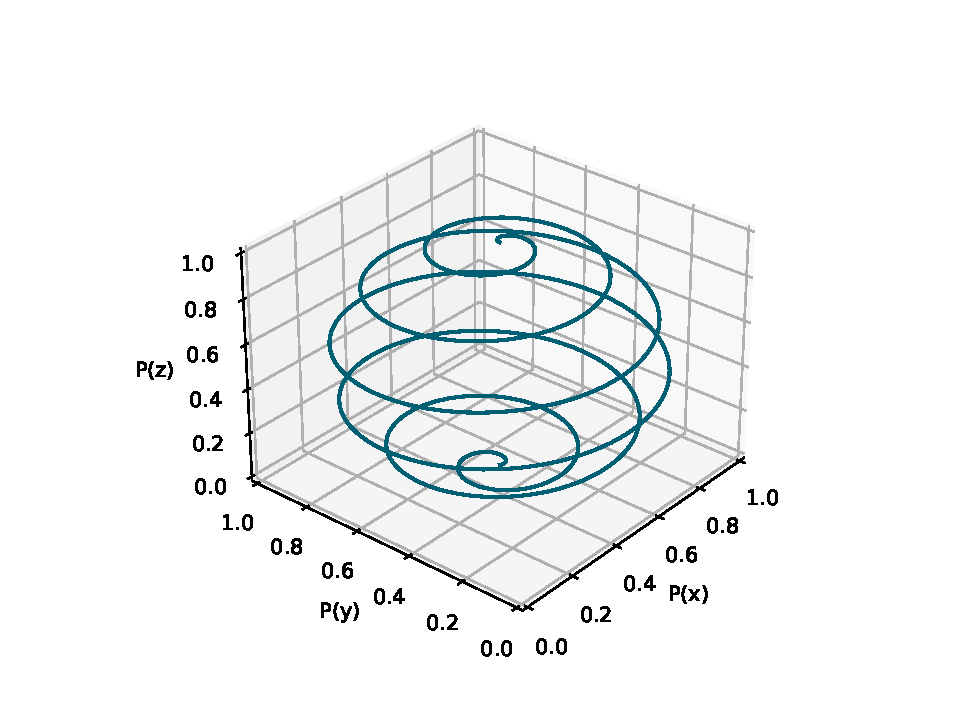
\includegraphics[width=\textwidth]{figures/rabi_pi.pdf}
\end{subfigure}%DO NOT REMOVE THIS '%'
\begin{subfigure}{.45\textwidth}
  \centering
  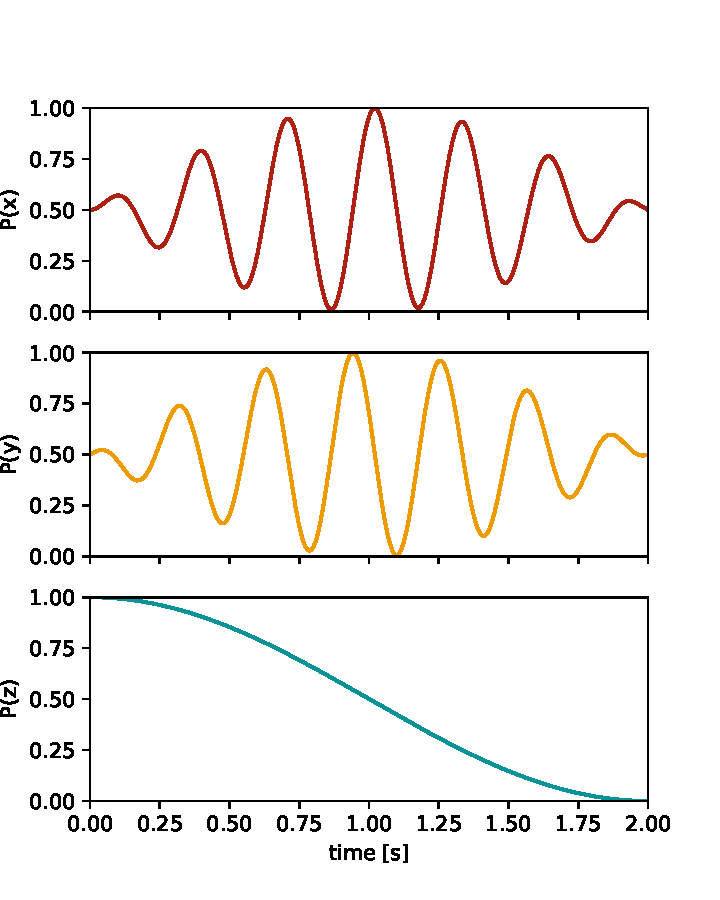
\includegraphics[width=0.9\textwidth]{figures/rabi_pi_px_py_pz.pdf}
\end{subfigure}
\caption
[Plot of an on-resonance Rabi sequence (``$\pi$ flip'') that transitions a neutron from spin up to spin down.]
{Plot of an on-resonance Rabi sequence (``$\pi$ flip'') that transitions a neutron from spin up to spin down. $P(x)$, $P(y)$, and $P(z)$ are the probabilities of measuring spin up along $x$, $y$, and $z$, given by Eqs.~(\ref{eq:rabi_circ_z}) \textendash ~(\ref{eq:rabi_circ_y}). Parameters: $\omega=\omega_0=\qty{20}{\radian\ \s^{-1}}$, $\omega_\text{c}=\pi/\qty{2}{\radian\ \s^{-1}}$, $\phi=\qty{0}{\radian}$, $t=\qty{2}{\s}$, $\Ket{\psi(t=0)}=\left( \begin{matrix}
    1 \\
    0
\end{matrix}\right)$}
\label{fig:rabi_circ_pi_pulse}
% \end{figure}

% \begin{figure}
% \centering
%subfigure width gets "multiplied" by includegraphics width
\begin{subfigure}{.55\textwidth} 
  \centering
  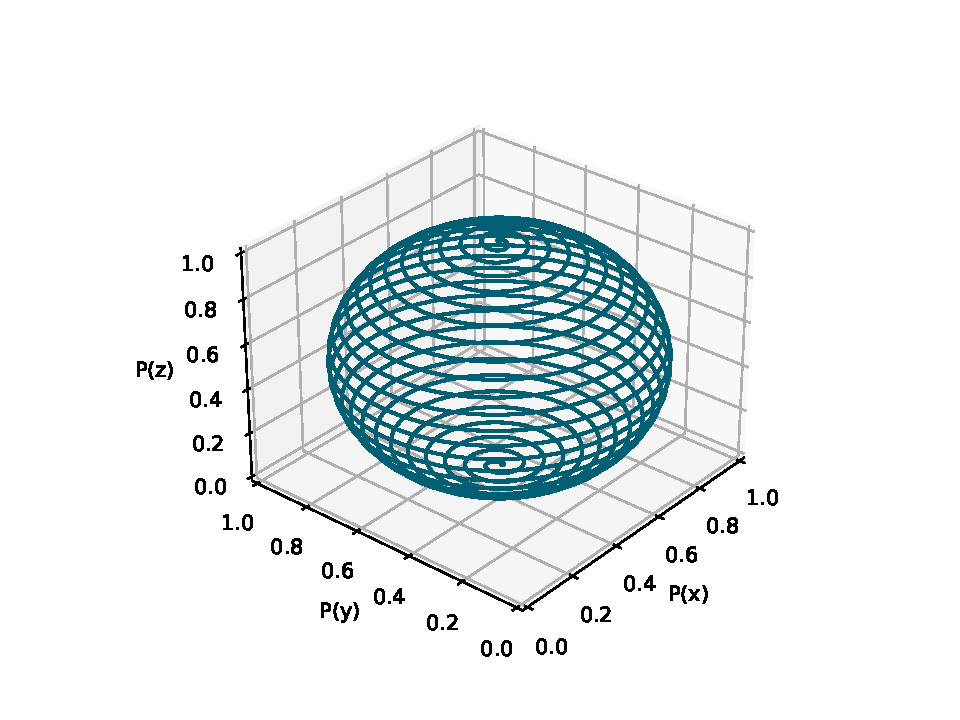
\includegraphics[width=\textwidth]{figures/rabi_linear.pdf}
\end{subfigure}%DO NOT REMOVE THIS '%'
\begin{subfigure}{.45\textwidth}
  \centering
  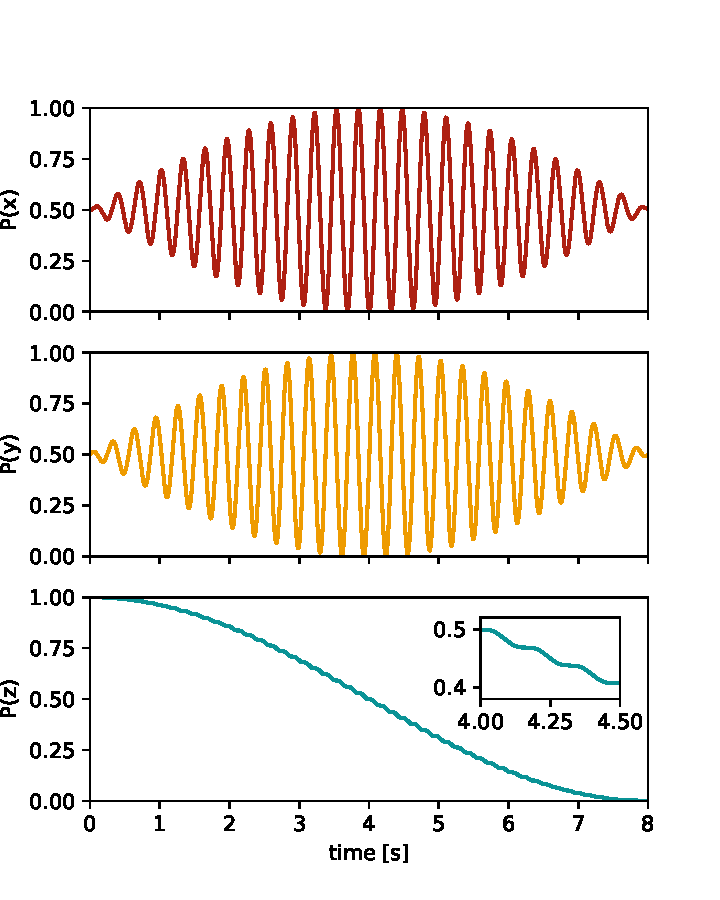
\includegraphics[width=0.9\textwidth]{figures/rabi_linear_px_py_pz.pdf}
\end{subfigure}
\caption
[Plot of an on-resonance Rabi sequence with a linear RF]
{Plot of an on-resonance Rabi sequence with a linear \acrshort{rf}. The spinor is solved with the numerical integration of Eqs.~(\ref{eq:rabi_linear_1}) and (\ref{eq:rabi_linear_2}). The inset on $P(z)$ shows an oscillating behavior not present in Fig.~\ref{fig:rabi_circ_pi_pulse}. Parameters: $\omega=\omega_0=\qty{20}{\radian\ \s^{-1}}$, $\omega_\text{c}=\pi/\qty{4}{\radian\ \s^{-1}}$, $\phi=\qty{0}{\radian}$, $t=\qty{8}{\s}$, $\Ket{\psi(t=0)}=\left( \begin{matrix}
    1 \\
    0
\end{matrix}\right)$}
\label{fig:rabi_linear_pi_pulse}
\end{figure}


%%%%%%%%%%%%%%%%%%%%%%%%%%%%%%%%%%%%%%%%%

\subsection{Rabi resonance with a linear RF field}

%%%%%%%%%%%%%%%%%%%%%%%%%%%%%%%%%%%%%%%%%

In an experimental setting it is more practical to generate a linear \acrshort*{rf} field. For a linear \acrshort*{rf} field $\vv{B_\ell}$ under the condition $B_\ell \ll B_0$, the magnetic field is now written as
%
\begin{gather}
    \vv{B}(t)=\vv{B_\ell}(t) + \vv{B_0}=B_\ell \cos (\omega t + \phi) \vv{x} + B_0 \vv{z}\label{eq:B0_with_linear_rf}
\end{gather}
%
We again let the frequency be $\omega_\ell=-\gamma B_\ell$. Following the procedure in Sec.~\ref{sec:rabi}, we use the \schrodinger equation to get
%
\begin{align}
    \dot{\psi}_+ &=\frac{-i}{2}\left( \omega_0 \psi_+ + \omega_\ell \psi_-  \cos(\omega t + \phi) \right)\label{eq:rabi_linear_1}\\
    \dot{\psi}_- &=\frac{i}{2}\left( \omega_0 \psi_- - \omega_\ell \psi_+ \cos(\omega t + \phi)  \right)\label{eq:rabi_linear_2}
\end{align}
%
This is solved numerically, as described in Appx.~\ref{appx:ramsey_numerical}.

As per Ref.~\cite{rabi_1938}, Rabi flips from a linear \acrshort*{rf} behave similarly to the result from  Sec.~\ref{sec:rabi} by the substitution 
%
\begin{gather}
    \frac{\omega_\ell}{2}\approx\omega_\text{c} \label{eq:linear_vs_circular_w}
\end{gather}
%
with a few caveats. Referring to a plot of a linear $\pi$ pulse (Fig.~\ref{fig:rabi_linear_pi_pulse}), the subplot for $P(z)=\left| \Braket{S_z;+ | \psi(t)} \right|^2 $ shows an oscillating artifact not present in the circular $\pi$ pulse (Fig.~\ref{fig:rabi_circ_pi_pulse}). Section~\ref{sec:bloch-siegert} further describes the distinction between circular and linear \acrshort*{rf} $\pi$ flips.

%%%%%%%%%%%%%%%%%%%%%%%%%%%%%%%%%%%%%%%%%

\subsection{Rabi fringe}\label{sec:rabi_fringe}

%%%%%%%%%%%%%%%%%%%%%%%%%%%%%%%%%%%%%%%%%

\begin{figure}
    \centering
    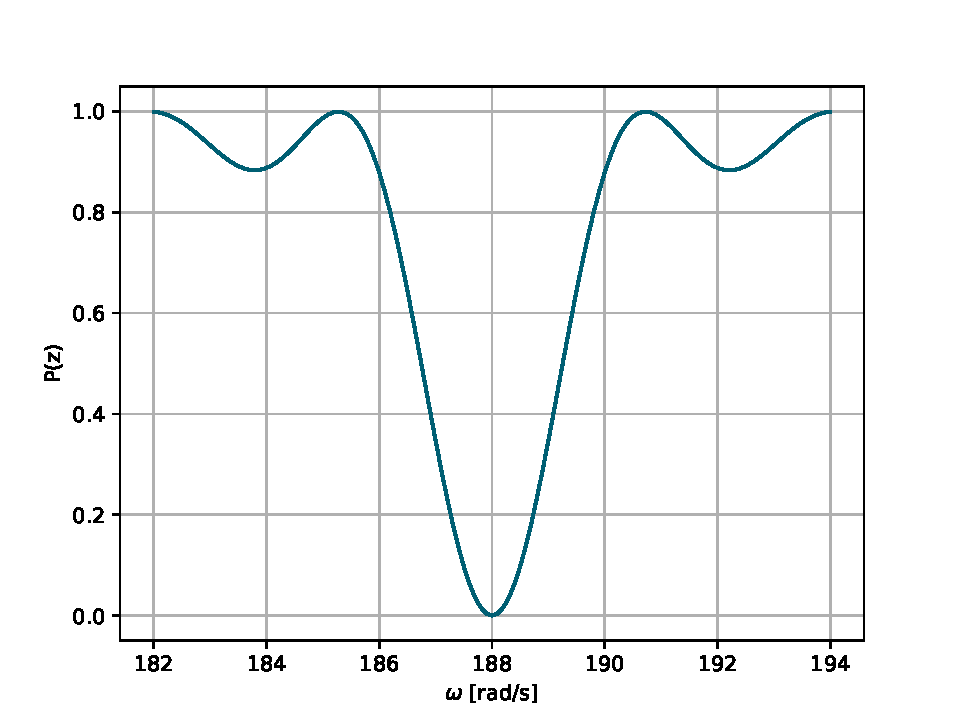
\includegraphics[width=0.6\textwidth]{figures/rabi_circ.pdf}
    \caption{A Rabi fringe, produced by repeatedly integrating Eqs.~(\ref{eq:rabi_2})\textendash (\ref{eq:rabi_3}) for various circular RF frequencies $\omega$. Here, $\omega_0=\qty{188}{\radian\ \s^{-1}}$, $\omega_\text{c}=\pi/\qty{2}{\radian\ \s^{-1}}$, and $t=\qty{2}{\s}$. The minimum is the resonant point where $\omega=\omega_0$}
    \label{fig:rabi_fringe_circ}
\end{figure}

Given knowledge of the static $B_0$ field ($\omega_0$) and the RF field strength ($\omega_\ell\text{ or }\omega_\text{c}$), performing a Rabi sequence for multiple RF frequencies ($\omega$) and counting the number of spin up neutrons produces a ``Rabi fringe'' (Fig.~\ref{fig:rabi_fringe_circ}). The minimum of the Rabi fringe, or the resonance, gives the precession frequency for the neutron in the static field $\omega=\omega_0$. 

For Rabi sequence $\pi$ pulse parameters that satisfy Eq.~(\ref{eq:rabi_pi_pulse_time}), the Rabi fringe is considered to be optimized, and the probability of measuring spin up along $z$ at the resonance point is 0.


%%%%%%%%%%%%%%%%%%%%%%%%%%%%%%%%%%%%%%%%%

\section{Bloch-Siegert Shift}\label{sec:bloch-siegert}

%%%%%%%%%%%%%%%%%%%%%%%%%%%%%%%%%%%%%%%%%

In 1940, Bloch and Siegert described an effect where using a linear \acrshort*{rf} instead of a circular \acrshort*{rf} for a Rabi flip slightly shifts the minimum of the resonant fringe \cite{bloch_magnetic_1940}. In summary, a linear \acrshort*{rf} may be thought of as a sum of two circular \acrshort*{rf}s with equal frequency, opposite directions of rotation, and half the field strength of the linear \acrshort*{rf}. This can be seen by making the substitution $\omega \rightarrow -\omega$ in Eq.~(\ref{eq:rabi_hamiltonian}) and observing that the sine term is odd while the cosine term is even. The presence of the second circular \acrshort*{rf} acts as a perturbation that shifts the resonance away from the Larmor frequency by some frequency $\Delta\omega_\text{Bloch}$. For a linear \acrshort*{rf}, the Bloch-Siegert shift is found in Refs.~\cite{bloch_magnetic_1940, ramsey_resonance_1955} to be constrained by
%
\begin{gather}
    \Delta\omega_\text{Bloch}= \frac{(\gamma B_\text{cr})^2}{4\omega_0} = \frac{\omega_\ell^2}{16\omega_0}\label{eq:bloch-siegert-prediction}
\end{gather}
%
where $B_\text{cr}$ is one of the counter-rotating circular \acrshort*{rf}s. 

Figure~\ref{fig:bloch-siegert-t} plots the numerically calculated $\Delta\omega_\text{Bloch}$ (Appx.~\ref{appx:ramsey_numerical}) as a function of pulse width $t_\pi$, with initial phase $\phi=0$. The numerical solution has the interesting feature of oscillating within bounds defined by Eq.~\ref{eq:bloch-siegert-prediction}, in agreement with the behavior of the numerical results obtained in Ref.~\cite{may_thesis}. As can be seen by Fig.~\ref{fig:bloch-siegert-phase} (albeit in the context of a Ramsey sequence, Sec.~\ref{sec:ramsey-method}), the initial phase $\phi$ also affects $\Delta\omega_\text{Bloch}$.

\begin{figure}
    \centering
    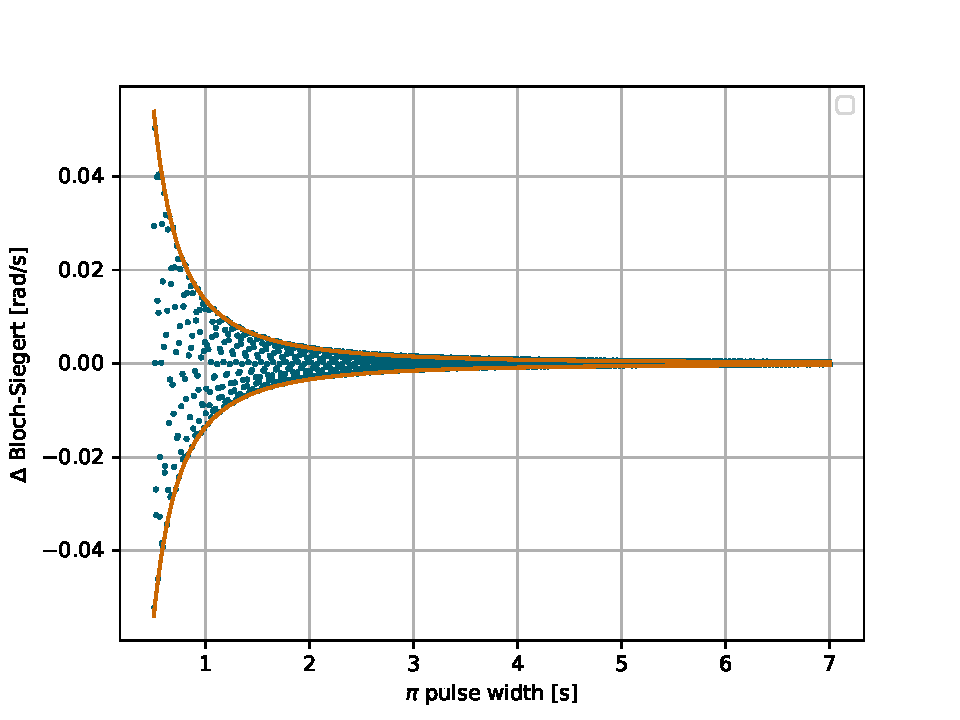
\includegraphics[width=0.7\textwidth]{figures/bloch-siegert-rabi.pdf}
    \caption
    [Bloch-Siegert shift as a function of pulse width $t_\pi$ for an optimized Rabi $\pi$ pulse. The \legendbox{burnt-orange-color} orange line corresponds to the prediction by Bloch and Siegert, Eq.~(\ref{eq:bloch-siegert-prediction}). The \legendbox{dark-blue-color} points are numerically calculated (Appx.~\ref{appx:ramsey_numerical})]
    {Bloch-Siegert shift as a function of pulse width $t_\pi$ for an optimized Rabi $\pi$ pulse. The \legendbox{burnt-orange-color} orange line corresponds to the prediction by Bloch and Siegert, Eq.~(\ref{eq:bloch-siegert-prediction}).  The \legendbox{dark-blue-color} points are numerically calculated (Appx.~\ref{appx:ramsey_numerical}). $\omega_0 \approx -183.247\,172 \text{ rad s}^{-1}$, where $\omega_\ell$ is determined by Eqs.~(\ref{eq:rabi_pi_pulse_time}) and (\ref{eq:linear_vs_circular_w}). Initial phase $\phi=0$. See discussion in Sec.~\ref{sec:bloch-siegert}.}
    \label{fig:bloch-siegert-t}
\end{figure}

\begin{figure}
    \centering
    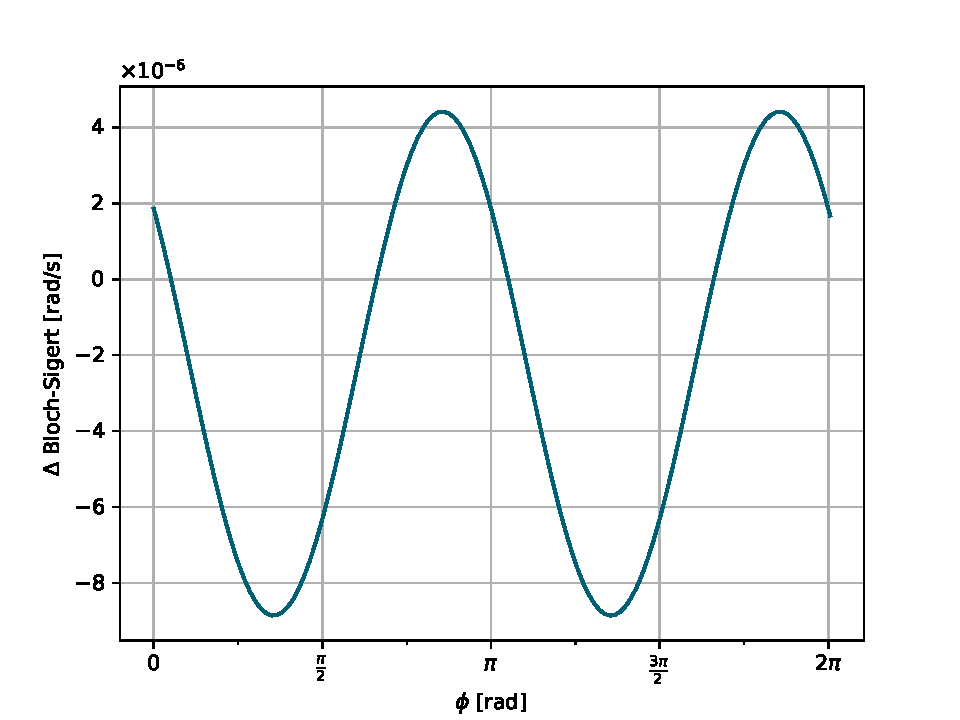
\includegraphics[width=0.7\textwidth]{figures/bloch-siegert-lanl-params.pdf}
    \caption
    {Numerically evaluated Bloch-Siegert shift (Appx.~\ref{appx:ramsey_numerical}) as a function of initial phase angle $\phi$ (\ref{eq:B0_with_linear_rf}) for a Ramsey fringe using the parameters in Sec.~\ref{sec:LANL_nEDM_ramsey_params}.}
    \label{fig:bloch-siegert-phase}
\end{figure}


%%%%%%%%%%%%%%%%%%%%%%%%%%%%%%%%%%%%%%%%%

\section{Ramsey method of separated oscillatory fields\label{sec:ramsey-method}}

%%%%%%%%%%%%%%%%%%%%%%%%%%%%%%%%%%%%%%%%%

\begin{figure}[htp]
    \centering
    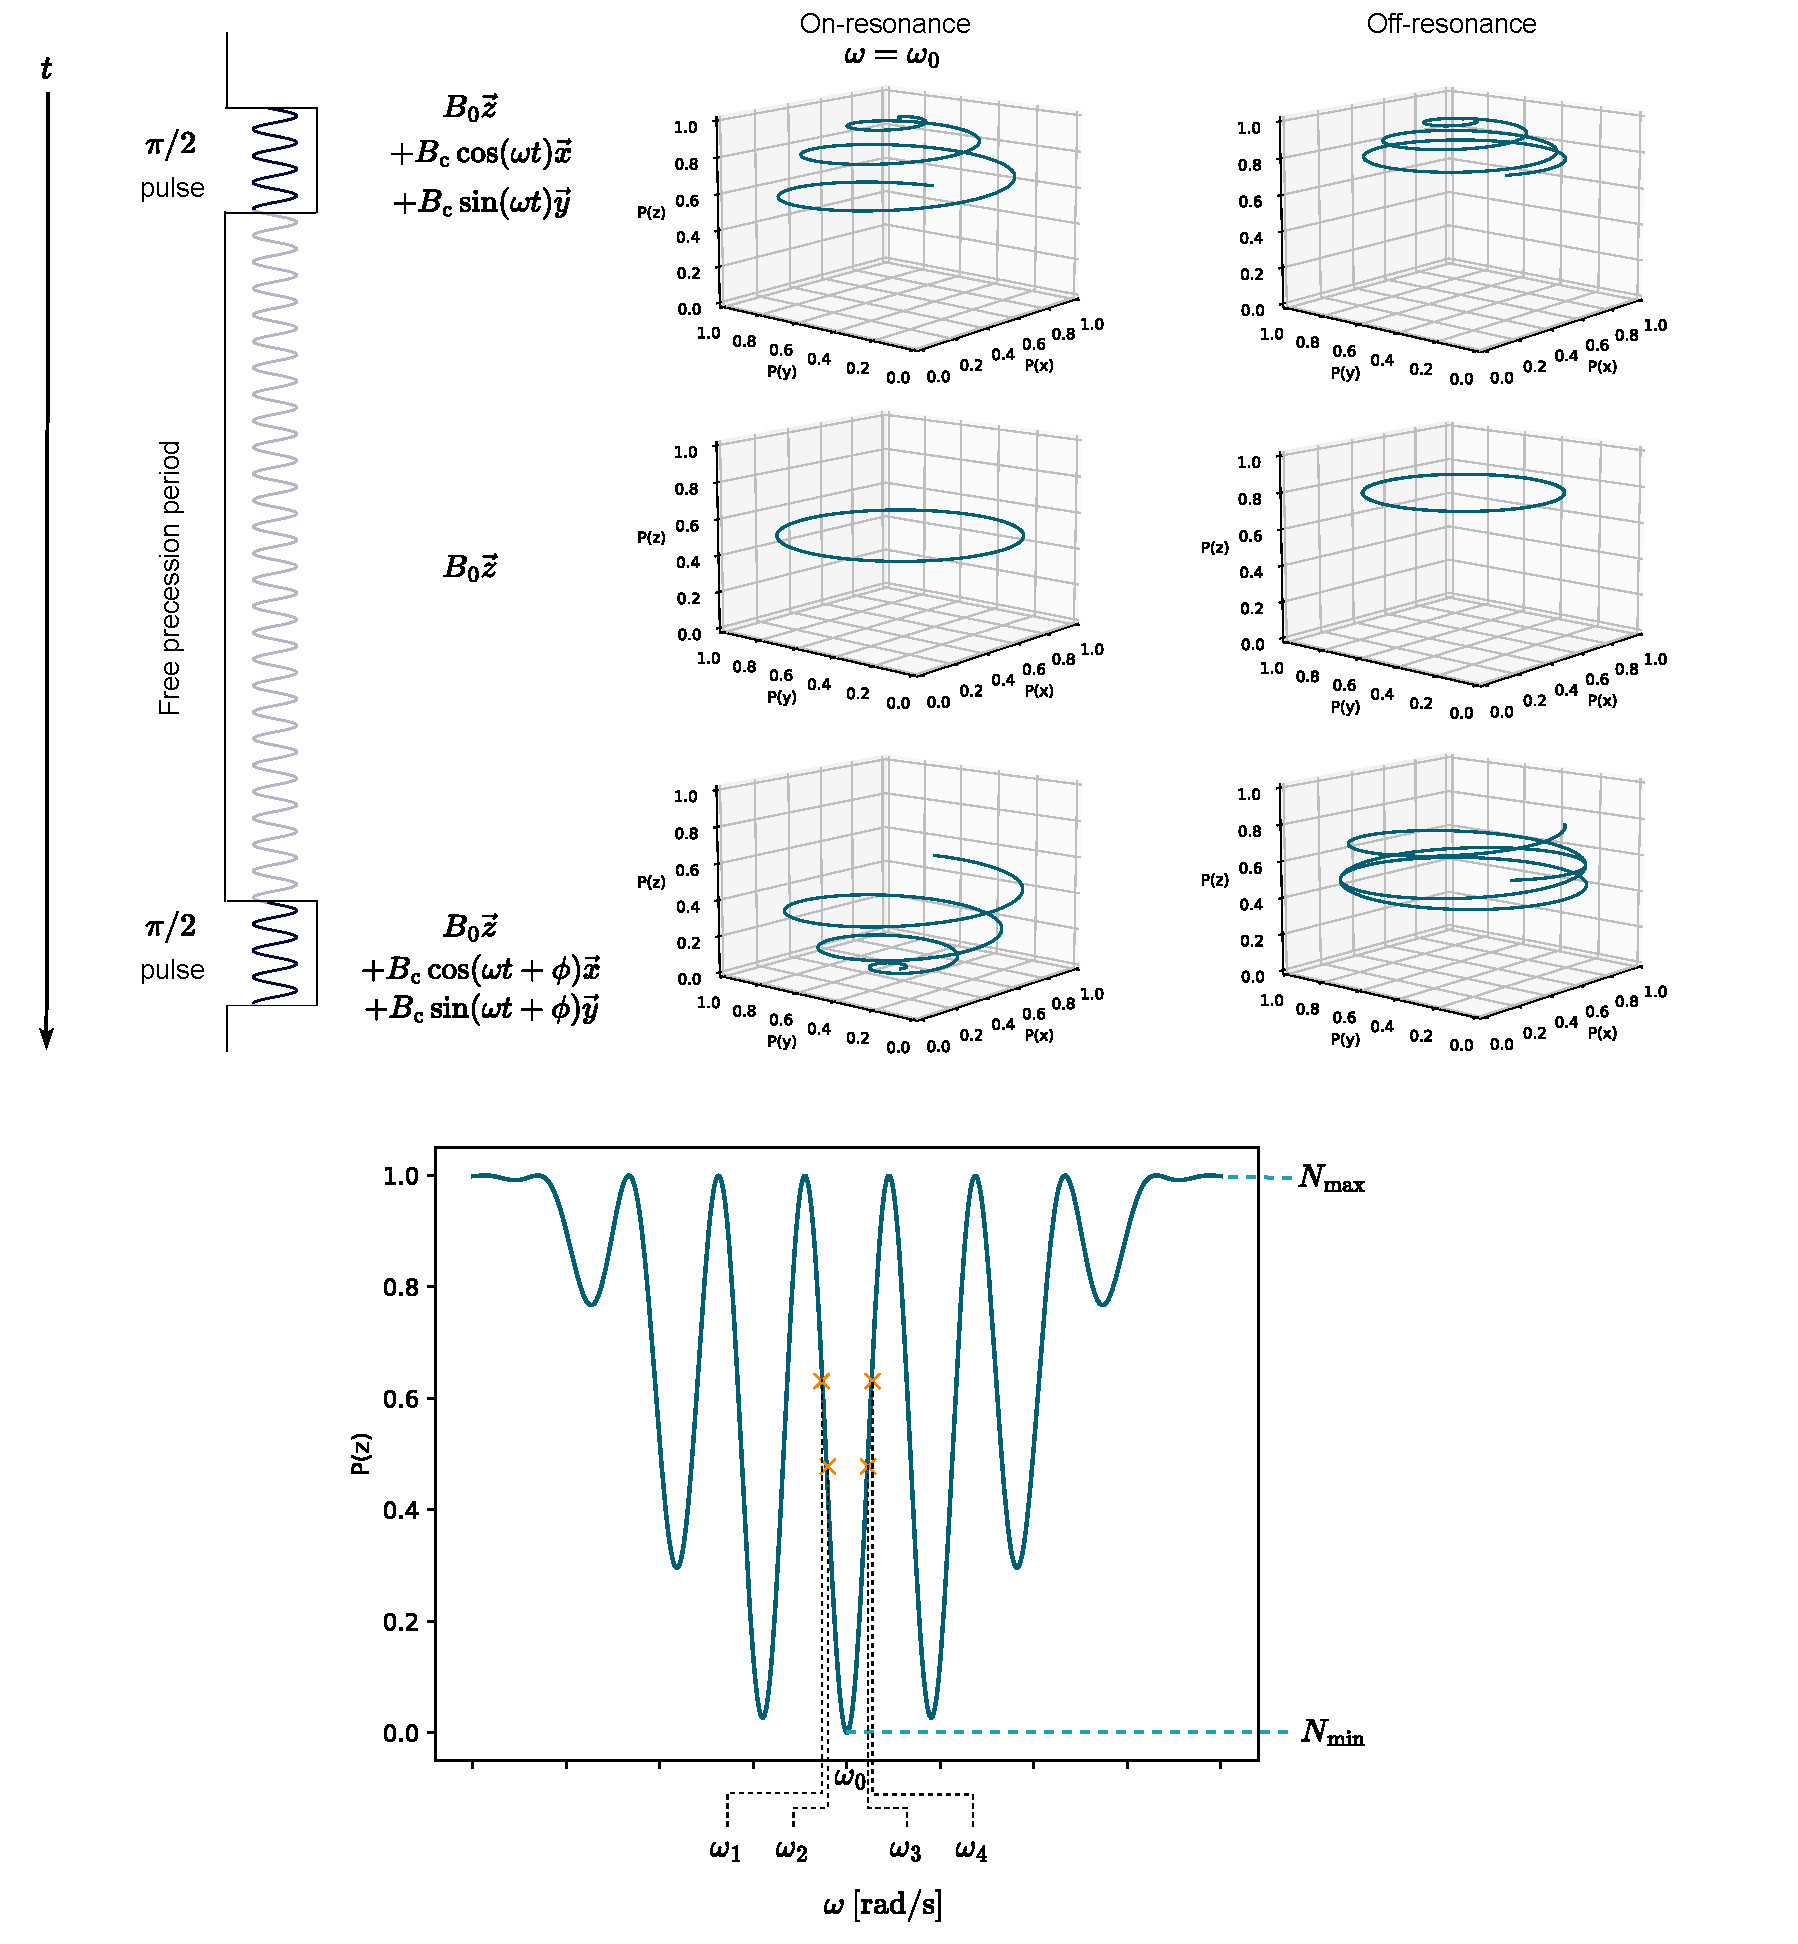
\includegraphics[width=\textwidth]{figures/ramsey_sequence.pdf}
    \caption[Illustration of two Ramsey sequences used in the production of the Ramsey fringe. The procedure is described in Sec.~\ref{sec:ramsey-method}]
    {Illustration of two Ramsey sequences used in the production of the Ramsey fringe. The procedure is described in Sec.~\ref{sec:ramsey-method}. $\omega_0$ is the circular RF frequency in the on-resonance sequence. $\omega_1$--$\omega_4$ are evenly distributed along the central fringe, used for fitting the resonance. $N_\text{min}$ is the number of spin up neutrons counted at resonance. $N_\text{max}$ is the number counted at a point far from resonance.}
    \label{fig:ramsey-sequence}
\end{figure}

The Ramsey method produces a narrower central peak than the Rabi method and gives higher resolution for determination of the resonant frequency. As depicted in Fig.~\ref{fig:ramsey-sequence}, the procedure for a Ramsey sequence as applied to an nEDM experiment is as follows:
%
\begin{enumerate}
    \item Beginning with a polarized population of \ucn, a magnetic field of the form (\ref{eq:B0_with_circular_rf}) or (\ref{eq:B0_with_linear_rf}) is applied for some time $t_{\pi/2}$ and a chosen RF frequency $\omega$. This is called a ``$\pi/2$ pulse.'' The optimized $\pi/2$ pulse width $t_{\pi/2}$ is determined by obtaining the $\pi$ pulse width $t_\pi$ from Eqs.~(\ref{eq:rabi_pi_pulse_time}) and (\ref{eq:linear_vs_circular_w}), then dividing $t_\pi$ by two.
    \item For a period \gls{T_fp}, the RF magnetic field is turned off ($B_\text{c}=B_\ell=0$). The \ucn are allowed to freely precess in the remaining static $B_0$ field.
    \item The magnetic RF field is switched on again for a duration $t_{\pi/2}$. This second $\pi/2$ pulse is in phase with the one described in the first step, such that $\phi = \omega ( t_{\pi/2} + \gls*{T_fp})$.
\end{enumerate}
%
The Ramsey sequence is then repeated for multiple RF frequencies $\omega$ to produce a Ramsey fringe.

Compared to width of the Rabi resonance, the Ramsey resonance narrows in proportion to the total time elapsed, and thus reduces the width by a factor of $\sim t_{\pi} / (T+2t_{\pi/2})$. More elaborate calculations of the full width half maximum (\acrshort*{fwhm}) give~\cite{may_thesis, pendlebury_revised_2015}
%
\begin{gather}
    \frac{1}{2 \gls*{T_fp}+8 t_{\pi/2} / \pi} \approx \frac{1}{2\gls*{T_fp}}
\end{gather}

The Ramsey method is particularly effective because it does not require the static $B_0$ field to be absolutely homogeneous within the spin precession region, because the resonant frequency is determined by the average $B_0$ field sampled by neutron spins during the free precession period. Of course, this assumes that transverse field gradients from the condition $\vv{\nabla}\cdot \vv{B}=0$ are within reason. Specific magnetic field uniformity requirements in the context of the LANL nEDM experiment are described in Sec.~\ref{sec:magnetic_field_req}.

Reference~\cite{ramsey_molecular_1950} provides the analytical solution for a Ramsey sequence using a circular RF magnetic field. The probability for a transition from a spin up state to spin down state is given by
%
\begin{gather}
    P_{\uparrow,\downarrow} = 4\sin^2\theta \sin^2\frac{at_{\pi/2}}{2}\left( \cos \frac{(\omega_0 - \omega)\gls*{T_fp}}{2}\cos\frac{at_{\pi/2}}{2}-\cos\theta \sin\frac{(\omega_0 - \omega)\gls*{T_fp}}{2}\sin\frac{at_{\pi/2}}{2} \right)^2 \label{eq:ramsey_1950_fringe_solution}
\end{gather}
%
where
%
\begin{align}
    \sin\theta &= \frac{\omega_\text{c}}{a} \\
    \cos\theta &= \frac{\omega_0 - \omega}{a} \\
    a &= \sqrt{(\omega_0-\omega)^2+\omega_\text{c}}
\end{align}

In the limit that $\omega_\text{c} \gg \omega_0 - \omega$ (the RF is close to resonance) and for $\omega_\text{c}t=\pi/2$ (resonant $\pi/2$ pulses), we have $a= \omega_\text{c}$, $\sin\theta= 1$, $\cos\theta=(\omega_0 - \omega)/\omega_\text{c}$, and $at_{\pi/2}/2=\pi/4$. This gives the simplified expression
%
\begin{gather}
    P_{\uparrow,\downarrow} \approx \cos^2\frac{(\omega - \omega_0)\gls*{T_fp}}{2} \label{eq:ramsey_1950_solution_simplified}
\end{gather}
%
To match more common notation we have changed $(\omega_0 - \omega)$ to $(\omega - \omega_0)$, which is mathematically equivalent in Eq.~(\ref{eq:ramsey_1950_solution_simplified}).

As with the Rabi sequence, there are only approximate analytical solutions to the Ramsey sequence with a linear RF magnetic field. A numerical solution for the linear RF is determined by applying Eqs.~(\ref{eq:rabi_linear_1})--(\ref{eq:rabi_linear_2}) for a period $t_{\pi/2}$, allowing the spinor the freely precess using for $\gls*{T_fp}$ with Eq.~(\ref{eq:larmor_solution}), then applying Eqs.~(\ref{eq:rabi_linear_1})--(\ref{eq:rabi_linear_2}) again for a period $t_{\pi/2}$ (implementation in Appx.~\ref{appx:ramsey_numerical}).

For a linear RF magnetic field, the Ramsey fringe is also subject to the Bloch-Siegert shift (Sec.~\ref{sec:bloch-siegert}). An estimate is provided in Ref.~\cite{code_bloch_siegert_1971}, but as demonstrated in Ref.~\cite{may_thesis} this prediction only provides a bounding envelope to values determined numerically. This is analogous to the case for the Rabi method shown in Fig.~\ref{fig:bloch-siegert-t}. Moreover, the prediction in \cite{code_bloch_siegert_1971} does not account for the Bloch-Siegert shift from initial phase $\phi$. Figure~\ref{fig:bloch-siegert-phase} demonstrates that varying $\phi$ alone will alter $\Delta\omega_\text{Bloch}$. 

We now consider a UCN spin polarizer (analyzer) with a finite efficiency $\epsilon$ for high field seekers to be transmitted to the detector. The number of neutrons counted at the end of the Ramsey sequence is
%
\begin{gather}
    N(\omega)= \epsilon N_\downarrow + (1 - \epsilon) N_\uparrow \label{eq:ramsey_finite_spin_analyzer}
\end{gather}
%
The quantities $N_\uparrow$ and $N_\downarrow$ change depending on the applied RF, as given by
%
\begin{align}
    N_\downarrow &= N_0 (1- P_{\uparrow,\downarrow} ) = N_0 \sin^2\frac{(\omega - \omega_0)\gls*{T_fp}}{2} \\
    N_\uparrow &= N_0 P_{\uparrow,\downarrow} = N_0 \cos^2\frac{(\omega - \omega_0)\gls*{T_fp}}{2}
\end{align}
%
where, $N_0$ is the number of stored polarized neutrons. In the fringe pattern, the maximum possible and minimum possible number of transmitted neutrons are
%
\begin{align}
    N_\text{max} &= \epsilon N_0\\
    N_\text{min} &= (1-\epsilon) N_0
\end{align}
%
As in Fig.~\ref{fig:ramsey-sequence}, $N_\text{max}$ is the number of neutrons measured at an \acrshort*{rf} frequency far from the resonance, and $N_\text{min}$ is the number measured at the resonance (which can be taken from a previous measurement cycle). 

We define the spin contrast of a Ramsey fringe \gls*{alpha} as
%
\begin{gather}
    \gls*{alpha} = \frac{N_\text{max} - N_\text{min}} {N_\text{max} + N_\text{min}} = 2\epsilon - 1 \label{eq:alpha}
\end{gather}
%
The spin contrast should be as close as possible to its maximum allowed value of $1$ to optimize statistical sensitivity of the experiment (see Sec.~\ref{sec:figure_of_merit}).

Equation~(\ref{eq:ramsey_finite_spin_analyzer}) can now be rewritten as
%
\begin{align}
    N(\omega) &= \epsilon N_0\sin^2 \frac{(\omega - \omega_0)\gls*{T_fp}}{2} + (1-\epsilon) N_0 \cos^2 \frac{(\omega - \omega_0)\gls*{T_fp}}{2} \\
    &= \epsilon N_0 - (2\epsilon - 1)N_0 \cos^2 \frac{(\omega - \omega_0)\gls*{T_fp}}{2} \\
    &= N_\text{max} - \gls*{alpha} N_0 \cos^2 \frac{(\omega - \omega_0)\gls*{T_fp}}{2}
\end{align}
%
and using $N_\text{max}=(\alpha + 1)N_0/2$, we have
%
\begin{align}
    N(\omega) &= \frac{N_0}{2}(\alpha + 1) - N_0\cos^2 \frac{(\omega - \omega_0)\gls*{T_fp}}{2} \\
    &= \frac{N_0}{2} - \frac{\alpha N_0}{2}\left( 2\cos^2 \frac{(\omega - \omega_0)\gls*{T_fp}}{2}-1\right) \\
    &= \frac{N_0}{2} \left( 1 - \alpha \cos\,(\omega - \omega_0)\gls*{T_fp} \right) \label{eq:ramsey_fringe_modulation_N_cos}
\end{align}


In practice, it is unnecessary to generate an entire Ramsey fringe for the determination of the resonant frequency. Four evenly-distributed points ($i=1,2,3,4$) along the central fringe are chosen where the slope is maximal, and are fitted with a function of the form~\cite{may_thesis}
%
\begin{gather}
    N(\omega_i)=N_\text{min} + (N_\text{max}-N_\text{min})\sin^2\left(\frac{\pi}{2\Gamma_\text{r}}(\omega_i-\omega_\text{r}) \right) \label{eq:four_point_ramsey_fringe_fit}
\end{gather}
%
where $\omega_\text{r}$ and $\Gamma_\text{r}$ are free parameters of the fit.




%%%%%%%%%%%%%%%%%%%%%%%%%%%%%%%%%%%%%%%%%

\subsection{Nominal Ramsey sequence parameters for the LANL nEDM}\label{sec:LANL_nEDM_ramsey_params}

%%%%%%%%%%%%%%%%%%%%%%%%%%%%%%%%%%%%%%%%%

The Ramsey sequence parameters utilized in the LANL nEDM experiment mirror those used in the measurement by Ref.~\cite{ABE20}, with the goal of producing the narrowest central fringe possible while also satisfying the magnetic field stability and uniformity requirements defined in Sec.~\ref{sec:magnetic_field_req}.
%
\begin{alignat}{3}
    B_0 &= 1\text{ \textmu T} \quad (\omega_0 \approx -183.247\,172 &&\text{ rad s}^{-1} ) \\
    B_\ell &= 4 \text{ nT} \quad (\omega_\ell \approx -0.732\,989 &&\text{ rad s}^{-1} ) \\
    \gls{T_fp} &= 180\text{ s} \\
    t_{\pi/2} &= 4.286\text{ s}
\end{alignat}
%
The high voltage electric field applied across the spin precession region is $E=\qty{12}{kV\per cm}$. The principles of an nEDM measurement using the Ramsey sequence are described in Sec.~\ref{sec:principles_nEDM}.

By convention, the primary uniform holding field along $\vv{z}$ for the Ramsey method is denoted as \gls*{b_0}. The strength of $B_0$ is largely chosen based on requirements for field uniformity and spin polarization lifetimes. If the primary contribution to non-uniformity comes from the $B_0$ coils, then smaller fields cause smaller gradients. Conversely, a stronger $B_0$ field improves adiabaticity (Sec.~\ref{sec:adiabaticity}), which leads to higher quality transport of \ucn spin into the experimental apparatus but at the cost of larger gradients in the precession area.



%%%%%%%%%%%%%%%%%%%%%%%%%%%%%%%%%%%%%%%%%

\section{Adiabaticity}\label{sec:adiabaticity}

%%%%%%%%%%%%%%%%%%%%%%%%%%%%%%%%%%%%%%%%%

Spin (when considered as a semiclassical vector) tends to ``follow'' the orientation of the local magnetic field as long as the field does not change too quickly. In particular, the motion of the spin depends on the Larmor precession frequency of the neutron $\omega_0$ relative to the rotation rate $\Omega$ of the local field $B$. This is quantified with the adiabaticity parameter $\gls*{adiab}$ \cite{abragam1961principles}
%
\begin{gather}
    \gls{adiab}=\left| \frac{\omega_0}{\Omega} \right| \label{eq:adiab}
\end{gather}
%
When $\gls*{adiab}\gg 1$, the the field changes slowly compared to the Larmor precession rate and the spin is able to adiabatically follow the field. When the adiabatic condition is not fulfilled ($\gls*{adiab}\not\gg 1$), the spin has increased difficulty staying aligned with the magnetic field and may be depolarized. For reference, the neutron gyromagnetic ratio \gls{gamma_n} (related to $\omega_0$ via Eq.~(\ref{eq:larmor_freq})) is roughly \qty{30}{\hertz.\micro\tesla^{-1}} \cite{codata_2018}.

The probability of depolarization is proportional $\exp(-\pi\eta)$ \cite{golubUCN}. Neutrons will also be depolarized by regions when the magnetic field is zero \cite{Majorana1932}. In the limit that the field changes drastically and quickly ($\gls*{adiab}\ll 1$), the spin vector of the neutron tends keep its direction fixed in space via the sudden approximation \cite{rabi_1936_space_quant}.

For a neutron with velocity $v$ traveling along $\vv{x}$, we can rewrite Eq.~(\ref{eq:adiab}) as
%
\begin{gather}
    \gls*{adiab}=\frac{ \gls{gamma_n}| \vv{B} |}{v\frac{d\theta}{dx}}
\end{gather}
%
where we define $\Omega$ such that $\Omega=d\theta/dt=v\,d\theta/dx$. The adiabaticity between two close points 1 and 2 is therefore
%
\begin{gather}
    \gls*{adiab}=\frac{\gls{gamma_n} \frac{ | \vv{B_2} | +| \vv{B_1}| }{2} | \vv{r_2} - \vv{r_1}|}
    {v\arccos \left( \frac{\vv{B_1}\cdot\vv{B_2}}{| \vv{B_1} | \, \vert \vv{B_2} | }\right)}
\end{gather}
%
An estimate of adiabaticity may also be written using the comparison of the Larmor frequency to the time variation of \gls*{bField}
%
\begin{gather}
    \gls*{adiab}=\frac{\gls{gamma_n}| \vv{B} | ^2}{\left| \frac{d\vv{B}}{dt} \right|}
    =\frac{\gls{gamma_n}| \vv{B} | ^2}{v\left| \frac{d\vv{B}}{dx} \right|}
\end{gather}
%
where we let the fractional rate of change of the field be $1/\tau = 1/ |\vv{B}|\,|d\vv{B}/dt|$.

%%%%%%%%%%%%%%%%%%%%%%%%%%%%%%%%%%%%%%%%%

\section{Adiabatic spin flipper}\label{sec:afp}

%%%%%%%%%%%%%%%%%%%%%%%%%%%%%%%%%%%%%%%%%

\begin{figure}[htp]
    \centering
    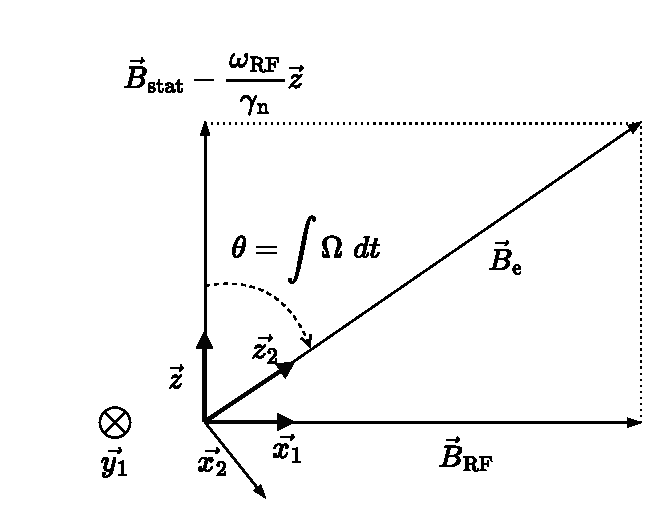
\includegraphics[width=0.5\textwidth]{figures/adiabatic_spin_flip.pdf}
    \caption[{Magnetic fields viewed in the frame of the neutron $\mathcal{R}_1$, which rotates at frequency $\omega_\text{RF}$ about $\vec{z}$}]
            {Magnetic fields viewed in the frame of the neutron $\mathcal{R}_1$, which rotates at frequency $\omega_\text{RF}$ about $\vv{z}$. $\vv{z}=\vv{z_1}$ and $\vv{y_1}=\vv{y_2}$}
    \label{fig:adiabatic_spin_flip}
\end{figure}

A fast adiabatic spin flipper (\acrshort{afp}) is used in the \acrshort*{lanl} \acrshort*{nedm} to provide the option of spin flipping \ucn before the spin analyzer and detector \cite{holley_afp_2012}. The \acrshort*{afp} spin flipper offers the benefit of spin flipping \ucn over a wide velocity range when adiabaticity conditions are satisfied. In this section, we reproduce the spin flip probability derivation from Refs.~\cite{robiscoe_spin_flip, grigoriev_neutron_2001, rogel_thesis}.

An \acrshort*{afp} spin flip requires two magnetic fields: (1)~A static field $\vv{B_\text{stat}}$ in the $\vv{z}$ direction with decreasing strength along $\vv{x}$, and (2)~an oscillating \acrshort{rf} field $\vv{B_\text{RF}}$ with frequency $\omega_\text{RF}$ perpendicular to $\vv{B_\text{stat}}$. Let $\vv{z}$ be the vertical direction, let $\vv{x}$ be the direction the neutron moves through the \acrshort*{afp} region at a velocity $v$, and let time $t=x/v$.

We first change from the lab frame $\mathcal{R}_0(\vv{x},\vv{y}, \vv{z})$ to a frame $\mathcal{R}_1(\vv{x_1},\vv{y_1}, \vv{z_1})$ moving with the neutron while also rotating about $\vv{z}$ at frequency $\omega_\text{RF}$ (see Fig.~\ref{fig:adiabatic_spin_flip}). In $\mathcal{R}_1$, the effective field $\vv{B_\text{e}}(t)$ seen by the neutron is given by
%
\begin{gather}
    \vv{B_\text{e}}(t)=\left(B_\text{stat}(t)-\frac{\omega_\text{RF}}{\gls{gamma_n}}\right)\vv{z}+B_\text{RF}(t)\vv{x} \label{eq:adiab_derivation_1}
\end{gather}
%
where in $\mathcal{R}_1$ we write $\vv{B_\text{RF}}=B_\text{RF}(t)\vv{x_1}$. The frame $\mathcal{R}_1$ is chosen such that:
%
\begin{enumerate}
    \item The static field term $\vv{B_\text{stat}}(t)$ gains a ficticious field term, $-\omega_\text{RF}/\gls{gamma_n}$ that arises from acceleration due to the rotation of the coordinate frame. At the resonance condition, $\vv{B_\text{stat}} = \vv{B_\text{RF}}$, the first two terms of Eq.~(\ref{eq:adiab_derivation_1}) cancel
    \item The neutron spin $\vv{S}(t)$ begins precession about $\vv{B_\text{RF}}$ (and effectively begins to follow $\vv{B_\text{e}}$ adiabatically)
\end{enumerate}
%
In the $\mathcal{R}_1$ frame, the Hamiltonian operator $\hat{H}$ with neutron magnetic moment operator $\hat{\gls{mu_n}}$ is
%
\begin{align}
    \hat{H} &= -\hat{\gls{mu_n}}\cdot\vv{B_{e}}=-\gls{gamma_n}\hat{S}\cdot\vv{B_{e}} \nonumber \\
    &= -\gls{gamma_n}\frac{\hbar}{2}\vv{\sigma}\cdot\vv{B_{e}}
\end{align}
%
Referring to Fig.~\ref{fig:adiabatic_spin_flip}, $\vv{B_\text{e}}(t)$ makes an angle $\theta(t)$ with the $\vv{z}$ axis. Therefore,
%
\begin{align}
    \vv{B_\text{e}}(t) &= B_\text{e}(t)\big(\sin\,\theta(t),\,0,\,\cos\,\theta(t) \big) \\
    \Rightarrow \hat{H} &= -\gls{gamma_n}\frac{\hbar}{2}B_\text{e}(t)\left[\left(\begin{matrix}
                0 & \sin \, \theta(t)\\
                \sin \, \theta(t) & 0
                \end{matrix}\right)+0+\left(\begin{matrix}
                \cos \, \theta(t) & 0\\
                0 & -\cos \, \theta(t)
                \end{matrix}\right)\right] \nonumber \\
    &= -\gls{gamma_n} \frac{\hbar}{2}B_\text{e}(t)\left(\begin{matrix}
                \cos \, \theta(t) & \sin \, \theta(t)\\
                \sin \, \theta(t) & -\cos \, \theta(t)
                \end{matrix}\right) \label{eq:adiab_derivation_2}
\end{align}
%
Writing the spinor as
$\Ket{\psi(t)}=\Ket{\begin{matrix}
    \psi_{+}(t)\\
    \psi_{-}(t)
\end{matrix}}$ and substituting Eq.~(\ref{eq:adiab_derivation_2}) into (\ref{eq:schrodinger}), the \schrodinger equation, gives
%
\begin{gather}
    \left(\begin{matrix}
    \dot{\psi_{+}}\\
    \dot{\psi_{-}}
    \end{matrix}\right)=\frac{i}{2}\gamma B_\text{e}(t)\left(\begin{matrix}
    \cos\, \theta(t) & \sin\, \theta(t)\\
    \sin\, \theta(t) & -\cos\, \theta(t)
    \end{matrix}\right)\left(\begin{matrix}
    \psi_{+}\\
    \psi_{-}
    \end{matrix}\right) \label{eq:adiab_derivation_3}
\end{gather}
%
Defining $\omega_\text{e}=-\gamma B_\text{e}$ as the precession frequency about $\vv{B_\text{e}}(t)$, we rewrite Eq.~(\ref{eq:adiab_derivation_3}) in the form
%
\begin{gather}
    \frac{d}{dt}\Ket{\psi(t)}=-\frac{i}{2}\omega_\text{e}\hat{M}\Ket{\psi(t)}
    \label{eq:adiab_derivation_4}
\end{gather}
%
We now change to the frame centered about the $\vv{z_2}$ axis. We use the rotation operator on ket space, $\mathcal{D}_y$, to rotate about the $\vv{y_1}$ axis to reach a reference frame we call $\mathcal{R}_2$. From Ref.~\cite{sakurai_quantum}, Eq.~(3.2.44), we have
%
\begin{align}
    \mathcal{D} &= \exp{\frac{-i\vv{\sigma}\hat{n}\phi}{2}}=\cos \, \frac{\phi}{2}
                            -i\vv{\sigma}\hat{n} \sin \, \frac{\phi}{2} \nonumber \\
                &= \left(\begin{matrix}\cos\left(\phi / 2\right)-i\hat{n_{z}}\sin\left(\phi / 2\right) & (-i\hat{n_{x}}-\hat{n_{y}})\sin\left(\phi / 2\right) \\
                (-i\hat{n_{x}}+\hat{n_{y}})\sin\left(\phi / 2\right) & \cos\left(\phi / 2\right)+i\hat{n_{z}}\sin\left(\phi / 2\right)
                \end{matrix}\right) \label{eq:rotation_operator}
\end{align}
%
A rotation about $\vv{y_1}$ with an angle $\theta(t)$ is therefore
%
\begin{align}
    \mathcal{{D}}_{y}=\left(\begin{matrix}
    \cos\left(\theta / 2\right) & -\sin\left(\theta / 2\right)\\
    \sin\left(\theta / 2\right) & \cos\left(\theta / 2\right)
    \end{matrix}\right)
\end{align}
%
Let us change frames to $\mathcal{R}_2$. We use the transformation $\Ket{\psi(t)}=\mathcal{{D}}_{y}\Ket{\psi'(t)}$, where $\psi'(t)$ is the spinor in frame $\mathcal{R}_2$. Recalling Eq.~(\ref{eq:adiab_derivation_4}) and using the chain rule,
%
\begin{align}
    \frac{d}{dt}\Ket{\psi(t)} &= -\frac{i}{2}\omega_\text{e}\hat{M}\Ket{\psi(t)} \nonumber \\
    \mathcal{{D}}_{y}\frac{d}{dt}\Ket{\psi'(t)}+\dot{\mathcal{{D}}_{y}}\Ket{\psi'(t)}&=-\frac{i}{2}\omega_{e}\hat{M}\mathcal{{D}}_{y}\Ket{\psi'(t)} \nonumber \\
    \frac{d}{dt}\Ket{\psi'(t)}&=-\frac{i}{2}\omega_{e}\mathcal{{D}}_{y}^{-1}\hat{M}\mathcal{{D}}_{y}\Ket{\psi'(t)}-\mathcal{{D}}_{y}^{-1}\dot{\mathcal{{D}}_{y}}\Ket{\psi'(t)}
    \label{eq:adiab_derivation_5}
\end{align}
%
In explicit matrix form, (\ref{eq:adiab_derivation_5}) is
\begin{align}
    \left(\begin{matrix}
    \dot{\psi'_{+}}\\
    \dot{\psi'_{-}}
    \end{matrix}\right)= & -\frac{i}{2}\omega_{e}\left(\begin{matrix}
    \cos\,\frac{\theta}{2} & \sin\,\frac{\theta}{2}\\
    -\sin\,\frac{\theta}{2} & \cos\,\frac{\theta}{2}
    \end{matrix}\right)\left(\begin{matrix}
    \cos\theta & \sin\theta\\
    \sin\theta & -\cos\theta
    \end{matrix}\right)\left(\begin{matrix}
    \cos\,\frac{\theta}{2} & -\sin\,\frac{\theta}{2}\\
    \sin\,\frac{\theta}{2} & \cos\,\frac{\theta}{2}
    \end{matrix}\right)\Ket{\psi'(t)} \nonumber \\
     & -\frac{\dot{\theta}}{2}\left(\begin{matrix}
    \cos\,\frac{\theta}{2} & \sin\,\frac{\theta}{2}\\
    -\sin\,\frac{\theta}{2} & \cos\,\frac{\theta}{2}
    \end{matrix}\right)\left(\begin{matrix}
    -\sin\,\frac{\theta}{2} & -\cos\,\frac{\theta}{2}\\
    \cos\,\frac{\theta}{2} & -\sin\,\frac{\theta}{2}
    \end{matrix}\right)\Ket{\psi'(t)} \nonumber \\
    = & -\frac{i}{2}\omega_{e}\left(\begin{matrix}
    1 & 0\\
    0 & -1
    \end{matrix}\right)\left(\begin{matrix}
    \psi'_{+}\\
    \psi'_{-}
    \end{matrix}\right)-\frac{\dot{\theta}}{2}\left(\begin{matrix}
    0 & -1\\
    1 & 0
    \end{matrix}\right)\left(\begin{matrix}
    \psi'_{+}\\
    \psi'_{-}
    \end{matrix}\right) \label{eq:adiab_derivation_6}
\end{align}
%
We are now in the frame $\mathcal{R}_2$, which follows $\vv{B_\text{e}}(t)$. Let us follow the motion of the neutron spin vector in this frame. Let the total angle of spin precession be $\lambda(t)=\int_0^t\omega_\text{e}(\tau)d\tau$. Again referring to Eq.~(\ref{eq:rotation_operator}), we now want a rotation of angle $\lambda(t)$ about axis $\vv{z_2}$. Let us call this frame $\mathcal{R}_3$. The rotation operator is
%
\begin{gather}
    \mathcal{{D}}_{z2}=\left(\begin{matrix}
    \cos\,\frac{\lambda}{2}-i\sin\,\frac{\lambda}{2} & 0\\
    0 & \cos\,\frac{\lambda}{2}+i\sin\,\frac{\lambda}{2}
    \end{matrix}\right)
    =\left(\begin{matrix}
    e^{-\frac{i}{2}\lambda} & 0\\
    0 & e^{\frac{i}{2}\lambda}
    \end{matrix}\right)
\end{gather}
%
Using the chain rule and the transformation $\Ket{\psi'(t)}=\mathcal{{D}}_{z2}\Ket{\psi''(t)}$
%
\begin{gather}
    \frac{d}{dt}\Ket{\psi''(t)}=\mathcal{{D}}_{z2}^{-1}\left(\frac{d}{dt}\Ket{\psi'(t)}\right)-\mathcal{{D}}_{z2}^{-1}\dot{\mathcal{{D}}_{z2}}\Ket{\psi''(t)}
    \label{eq:adiab_derivation_7}
\end{gather}
%
Here, we know $\frac{d}{dt}\Ket{\psi'(t)}$ from Eq.~(\ref{eq:adiab_derivation_6}). Substituting into Eq.~(\ref{eq:adiab_derivation_7}) gives
%
\begin{align}
    \frac{d}{dt}\Ket{\psi''(t)}= & \mathcal{{D}}_{z2}^{-1}\left[-\frac{i}{2}\omega_{e}\left(\begin{matrix}
    1 & 0\\
    0 & -1
    \end{matrix}\right)\left(\begin{matrix}
    \psi'_{+}\\
    \psi'_{-}
    \end{matrix}\right)-\frac{\dot{\theta}}{2}\left(\begin{matrix}
    0 & -1\\
    1 & 0
    \end{matrix}\right)\left(\begin{matrix}
    \psi'_{+}\\
    \psi'_{-}
    \end{matrix}\right)\right] \nonumber \\
     & -\mathcal{{D}}_{z2}^{-1}\dot{\mathcal{{D}}_{z2}}\Ket{\psi''(t)}
     \label{eq:adiab_derivation_8}
\end{align}
%
where
%
\begin{gather}
    \mathcal{{D}}_{z2}^{-1}=\left(\begin{matrix}
    e^{\frac{i}{2}\lambda} & 0\\
    0 & e^{-\frac{i}{2}\lambda}
    \end{matrix}\right),\quad\dot{\mathcal{{D}}_{z2}}=\frac{\dot{\lambda}}{2}\left(\begin{matrix}
    -ie^{-\frac{i}{2}\lambda} & 0\\
    0 & ie^{\frac{i}{2}\lambda}
    \end{matrix}\right),\nonumber\\
    \text{ and} \quad \mathcal{{D}}_{z2}^{-1}\dot{\mathcal{{D}}_{z2}}=\frac{i\dot{\lambda}}{2}\left(\begin{matrix}
    -1 & 0\\
    0 & 1
    \end{matrix}\right).\nonumber
\end{gather}
%
Observing that $\dot{\lambda}=\omega_\text{e}$ and $\Ket{\psi'(t)}=\mathcal{{D}}_{z2}\Ket{\psi''(t)}$, the first and third terms of Eq.~(\ref{eq:adiab_derivation_8}) cancel out. This leaves
%
\begin{gather}
    \frac{d}{dt}\Ket{\psi''(t)}=\frac{\dot{\theta}}{2}\left(\begin{matrix}
    0 & e^{\frac{i}{2}\lambda}\\
    -e^{-\frac{i}{2}\lambda} & 0
    \end{matrix}\right)\left(\begin{matrix}
    \psi'_{+}\\
    \psi'_{-}
    \end{matrix}\right)\label{eq:adiab_derivation_9}
\end{gather}
%
To solve for Eq.~(\ref{eq:adiab_derivation_9}), we must change to $\theta$ as the independent variable. $\lambda$ becomes a function of $\theta$ by the adiabatic parameter \gls{adiab} introduced in Sec.~\ref{sec:adiabaticity}. 
%
\begin{gather}
\lambda =\int_{0}^{t}\omega_{e}(\tau)d\tau
 =\int_{0}^{\theta}\frac{\omega_{e}}{\dot{\theta}}d\theta
 =\int_{0}^{\theta}\gls*{adiab}(\theta)d\theta
 \label{eq:adiab_derivation_10}
\end{gather}
%
where we used the relations $\dot{\theta}=d\theta/d\tau,\,\,\gls*{adiab}(t)=\left|\omega_\text{e}/\Omega(t)\right|,$ and let the rotation rate of $\vv{B_\text{e}}(t)$ be $\Omega(t)=\dot{\theta}$. Eq.~(\ref{eq:adiab_derivation_9}) becomes
%
\begin{align}
\frac{d\psi''_{+}}{d\theta}= & \frac{1}{2}e^{-\lambda}\psi''_{-}
\label{eq:adiab_derivation_11}\\
\frac{d\psi''_{-}}{d\theta}= & -\frac{1}{2}e^{-i\lambda}\psi''_{+}
\label{eq:adiab_derivation_12}
\end{align}
%
To decouple, we take another derivative with respect to $\theta$ to obtain $d^2\psi''_{+}/d\theta^2$ and $d^2\psi''_{-}/d\theta^2$. Then we use $\dot{\lambda}=\gls*{adiab}(\theta)$, (\ref{eq:adiab_derivation_11}), and (\ref{eq:adiab_derivation_12}) to obtain the last set of equations that need to be solved,
%
\begin{align}
\frac{d^{2}\psi''_{+}}{d\theta^{2}}-i\gls*{adiab}\frac{d\psi''_{+}}{d\theta}+\frac{1}{4}\psi''_{+} & =0\\
\frac{d^{2}\psi''_{-}}{d\theta^{2}}+i\gls*{adiab}\frac{d\psi''_{-}}{d\theta}+\frac{1}{4}\psi''_{-} & =0
\end{align}
%
which, for constant \gls{adiab}, has a solution of the form
%
\begin{gather}
    \psi''_\pm=\exp\left( \pm \frac{i\gls*{adiab}\theta}{2} \right)
                \left[C_{\psi\pm}\cos \left(\frac{\theta}{2}\sqrt{1+\gls*{adiab}^2} \right)  
                + i D_{\psi\pm}\sin \left(\frac{\theta}{2}\sqrt{1+\gls*{adiab}^2} \right)
                \right]
\end{gather}
%
At time $t=0$, we have $\theta=0$, and the neutron is in an initial unflipped state $\psi_+=1,\,\,\psi_-=0$. To translate these initial conditions from $\mathcal{{R}}_{1}\rightarrow\mathcal{{R}}_{3}$, from our rotation operators we have
%
\begin{gather}   
    \Ket{\psi(t)}=\mathcal{{D}}_{y}\Ket{\psi'(t)}=\mathcal{{D}}_{y}\mathcal{{D}}_{z2}\Ket{\psi''(t)} \\
    \Rightarrow\Ket{\psi''(t)}=\mathcal{{D}}_{z2}^{-1}\mathcal{{D}}_{y}^{-1}\Ket{\psi(t)}
    \label{eq:adiab_derivation_13}
\end{gather}
%
Solving for initial conditions gives
%
\begin{align}
    \psi''_{+} &= e^{\frac{i\gls*{adiab}\theta}{2}}\left(\cos\left(\frac{\theta}{2}\sqrt{1+\gls*{adiab}^{2}}\right)-\frac{i\gls*{adiab}}{\sqrt{1+\gls*{adiab}^{2}}}\sin\left(\frac{\theta}{2}\sqrt{1+\gls*{adiab}^{2}}\right)\right) 
    \label{eq:adiab_derivation_14}\\
    \psi''_{-} &= -\frac{\exp\left(-\frac{i\gls*{adiab}\theta}{2}\right)}{\sqrt{1+\gls*{adiab}^{2}}}\sin\left(\frac{\theta}{2}\sqrt{1+\gls*{adiab}^{2}}\right)
    \label{eq:adiab_derivation_15}
\end{align}
%
Finally, using (\ref{eq:adiab_derivation_13}), (\ref{eq:adiab_derivation_14}), and (\ref{eq:adiab_derivation_15}) to obtain $\Ket{\psi}$, and examining when the field $\vv{B_\text{e}}$ has turned by $\pi$ radians,
%
\begin{align}
    |\psi_{+}|^{2} &= \frac{1}{1+\gls*{adiab}^{2}}\sin^{2}\left(\frac{\pi}{2}\sqrt{1+\gls*{adiab}^{2}}\right) \\
    |\psi_{-}|^{2} &= 1-|\psi_{+}|^{2} \label{eq:adiab_derivation_16}
\end{align}
%
In this section the adiabaticity parameter is written in terms of precession about the effective field $\vv{B_\text{e}}$ and the rotation rate of the effective field 
%
\begin{gather}
    \gls*{adiab}(t)=\left|\frac{\omega_\text{e}}{\Omega(t)}\right| \label{eq:adiab_AFP}
\end{gather}
%
This differs slightly from the version introduced in Sec.~\ref{sec:adiabaticity}, which is written in terms of a more general local field. Let us write a more practical definition for spin flipper adiabaticity. For the amplitude of the \acrshort*{rf} field along the neutron path $x=[0,\ell_0]$, we can write the form \cite{grigoriev_neutron_2001}
%
\begin{gather}
    B_\text{RF}=A\sin \left(\pi \frac{x}{\ell_0}\right) = A\sin \left(\pi \frac{vt}{\ell_0}\right)\label{eq:adiab_derivation_17}
\end{gather}
%
$A$ is the modulation amplitude and $\ell_0$ is the the length of the flipper. We let $B_0$ be the field in the center of the flipper $x_0=\ell_0/2$, so that we may write the static field amplitude as
%
\begin{gather}
    B_\text{stat}=B_0 + A\cos\left(\pi \frac{x}{\ell_0}\right) =B_0 + A\cos\left(\pi \frac{vt}{\ell_0}\right)\label{eq:adiab_derivation_18}
\end{gather}
%
The second term of Eq.~(\ref{eq:adiab_derivation_18}) manifests as a permanent gradient field superimposed onto a uniform field $B_0$. From Fig.~\ref{fig:adiabatic_spin_flip}, we also have
%
\begin{gather}
    B_\text{e}=\sqrt{B_\text{RF}^2+\left(B_\text{stat}-\frac{\omega_\text{RF}}{\gls*{gamma_n}} \right)^2}
\end{gather}
%
Again referring to Fig.~\ref{fig:adiabatic_spin_flip}, we find $\Omega$ to be
%
\begin{align}
    \Omega(t) &= \frac{d\theta}{dt}= \frac{d}{dt}\left( \arcsin \frac{B_\text{RF}}{B_\text{e}} \right) = 
    \frac{B_\text{e}\dot{B}_\text{RF}-B_\text{RF}\dot{B}_\text{e}}
    {B_\text{e}^2\sqrt{1-(B_\text{RF}/B_\text{e})^2}} \\
    &\approx \frac{\left(B_\text{stat}-\frac{\omega_\text{rf}}{\gls*{gamma_n}} \right)\dot{B}_\text{RF}-B_\text{RF}\dot{B}_\text{stat}}
    {B_\text{e}^2}
     \label{eq:adiab_derivation_19}
\end{align}
%
At the resonant point, we have $t_0=\ell_0/(2v)$ and $B_0=\omega_\text{RF}/\gls*{gamma_n}$. Therefore, using Eqs.~(\ref{eq:adiab_derivation_17}), (\ref{eq:adiab_derivation_18}), and (\ref{eq:adiab_derivation_19}), Eq.~(\ref{eq:adiab_AFP}) becomes
%
\begin{gather}
    \gls*{adiab} = \frac{\gls*{gamma_n} \ell_0 A}{\pi v}
\end{gather}
%
Eq.~(\ref{eq:adiab_derivation_16}) gives the chance of measuring a different spin state after the neutron has passed through the spin flipper region (i.e., $\vv{S}$ has followed $\vv{B_\text{e}}$ adiabatically). For constant \gls*{adiab}, the spin flip probability is
%
\begin{gather}
    P=1-\frac{1}{1+\gls*{adiab}^{2}}\sin^{2}\left(\frac{\pi}{2}\sqrt{1+\gls*{adiab}^{2}}\right)
\end{gather}

As can be inferred from Eq.~(\ref{eq:adiab_derivation_1}), the resonant frequency for optimized spin flipping is given by $\gls{gamma_n} B_\text{stat}(\ell_0/2)$, where $B_\text{stat}(\ell_0/2)$ is the static field at the center of the RF coil and $\gls{gamma_n} \approx \qty{30}{MHz \per T}$.

%%%%%%%%%%%%%%%%%%%%%%%%%%%%%%%%%%%%%%%%%

\section{Bloch equations}\label{sec:bloch_equations}

%%%%%%%%%%%%%%%%%%%%%%%%%%%%%%%%%%%%%%%%%

Thus far we have relied upon a quantum mechanical description of spin interacting with a magnetic field. In certain cases it is more convenient to consider the semi-classical limit. A magnetic field $\vv{B}$ exerts a torque on the spin of the neutron, which causes the evolution of spin over time. This motion is described by the Bloch equations
%
\begin{gather}
    \frac{d\vv{S}}{dt}=\gls{gamma_n}\vv{S}\times \vv{B}
    \label{eq:bloch_equations}
\end{gather}
%
The results of Secs.~\ref{sec:larmor}\textendash \ref{sec:ramsey-method} and \ref{sec:spin_flipper_analyzer} may be reproduced by the Bloch equations.

%%%%%%%%%%%%%%%%%%%%%%%%%%%%%%%%%%%%%%%%%

\subsection{Spin relaxation}\label{sec:spin_relaxation}

%%%%%%%%%%%%%%%%%%%%%%%%%%%%%%%%%%%%%%%%%

The effects of spin relaxation can be introduced into Eq.~(\ref{eq:bloch_equations}) for some decaying polarization of the form $P(t)=P_0 \exp(-t/T_i)$. We define longitudinal $(z)$ relaxation time $T_1$, related to how long a population of polarized \ucn spins can stay coherent. We also define the transverse $(xy)$ depolarization time $T_2$, related to how long a population of precessing \ucn spins can stay coherent. For an ensemble of spins, assuming the main field direction is along $z$, the Bloch equations become
%
\begin{align}
    \frac{d\vv{S}_{x,y}}{dt} &= \gls{gamma_n} (\vv{S} \times \vv{B})_{x,y}-\frac{S_{x,y}}{T_2} \\
    \frac{d\vv{S}_z}{dt} &= \gls{gamma_n} (\vv{S} \times \vv{B})_{z}-\frac{S_z-S_0}{T_1}
\end{align}
%
where $S_0$ is the spin along axis $z$ at $t=0$.

Reference~\cite{mcgregor_transverse_1990} details the relationship of magnetic field gradients to spin relaxation. The formalism can be adapted to describe longitudinal relaxation time as a function of the vertical field gradient in a precession cell
%
\begin{gather}
    \frac{1}{T_1}=\frac{\gls{gamma_n} \overline{v}^2 \tau_\text{c}}{2\omega_0^2(1+\omega_0^2\tau_\text{c}^2)}\left(\frac{\partial B_0}{\partial z}\right)^2 \label{eq:T1_dBdZ_mcgregor}
\end{gather}
%
where $\tau_\text{c}=4V/(\overline{v} A)$ (from Appx.~\ref{appx:ucn_effusion}) is the average time between wall collisions, $V$ is the cell volume, $A$ is the inner surface area of the cell, $\overline{v}$ is the average velocity in the cell, $\omega_0$ is the Larmor precession frequency of the particle in $B_0\vv{z}$, and $\partial B/\partial z$ is the vertical gradient of the magnetic field. We make the assumption in (\ref{eq:T1_dBdZ_mcgregor}) that the $x$ and $y$ gradients are equal, and use $\vv{\nabla}\cdot \vv{B}_0=0$ to rewrite the formalism in terms of vertical gradient.

Transverse relaxation time for a cylindrical cell of height $H$ and radius $R$ is written as~\cite{mcgregor_transverse_1990}
%
\begin{gather}
    \frac{1}{T_2}=\frac{1}{2T_1}+\frac{\gls{gamma_n}^2 H^4}{120\,D}\left(\frac{\partial B_z}{\partial x}\right)^2 + \frac{7\gls{gamma_n}^2 R^4}{96\,D}\left( \frac{\partial B_z}{\partial y} \right)^2
    \label{eq:T2_mcgregor}
\end{gather}
%
for some diffusion constant $D$. For \ucn, Eq.~(4.71) in Ref.~\cite{golubUCN} gives the estimate
%
\begin{gather}
    D_\text{ucn}=\frac{\overline{v}\overline{l}_0^2}{2\overline{\lambda}}\label{eq:ucn_diffusion_constant}
\end{gather}
%
where $\overline{\lambda}$ is the mean free path for diffuse collisions and $\overline{l}_0$ is the average distance between wall collisions. For a cell of volume $V$ and inner surface area $A$, we have $\overline{l}_0=4V/A$~\cite{bate_mfp_1947}. We note that Eqs.~(\ref{eq:T1_dBdZ_mcgregor}) and (\ref{eq:T2_mcgregor}) assume no depolarization from wall collisions.

%%%%%%%%%%%%%%%%%%%%%%%%%%%%%%%%%%%%%%%%%

\section{Bargmann-Michel-Telegdi equation}\label{sec:BMT_equations}

%%%%%%%%%%%%%%%%%%%%%%%%%%%%%%%%%%%%%%%%%

The Bloch equations hold in the rest frame of the neutron, but transforming to the laboratory frame with relativistic corrections is more complicated. The motion of spin in the lab frame is described by the Bargmann-Michel-Telegdi (BMT) equation~\cite{bmt_equations}.
%
\begin{align}
    \frac{d\vv{S}}{dt} &= \left( \frac{\gamma}{\gls*{lorentz}}\vv{B'}+\vv{\omega_\text{T}}\right)\times \vv{S}\\
    \vv{B'} &= \vv{B}_\parallel + \gls*{lorentz}\vv{B}_\perp - \frac{\gls*{lorentz}}{c^2}\frac{d\vv{x}}{dt}\times\vv{E}\\
    \vv{\omega_\text{T}}&=\frac{\gls*{lorentz}^2}{c^2(1+\gls*{lorentz})}\frac{d^2\vv{x}}{dt^2}\times\frac{d\vv{x}}{dt}
\end{align}
%
where $\omega_\text{T}$ is the Thomas precession frequency, $B'$ is the magnetic field in the rest frame of the particle, $\gamma$ is the gyromagnetic ratio, and the Lorentz factor is $\gls*{lorentz}=\glsvalue*{lorentz}$. The transverse and longitudinal magnetic field components in the laboratory frame $B_\parallel$ and $B_\perp$ are defined with respect to the particle traveling along $x$.

Relativistic corrections are not necessary for spin tracking simulations of \ucn, but \pentrack (Chap.~\ref{chap:simulations}) implements this formulation to support particles such as electrons and protons.
%%%%%%%%%%%%%%%%%%%%%%%%%%%%%%%%%%%%%%%%%

\chapter{The LANL nEDM experiment}\label{chap:LANL_nEDM}

%%%%%%%%%%%%%%%%%%%%%%%%%%%%%%%%%%%%%%%%%

At the Los Alamos National Laboratory (LANL), a solid deuterium (SD$_2$) based superthermal UCN source coupled to a spallation target has been providing UCN to experiments for the last 20 years (Fig.~\ref{fig:AreaB_schematic})~\cite{saunders_performance_2013, ito_performance_2018}. The UCN source (Sec.~\ref{sec:lanl_ucn_source}) was upgraded to host a new nEDM experiment that will use Ramsey's method of separated oscillatory fields to search for the nEDM with an uncertainty goal of $\delta \gls*{d_n} = 2.7\times 10^{-27}$~$e\cdot\text{cm}$ (Sec.~\ref{sec:lanl_nedm_uncertainty}).

In this chapter we provide an overview of LANL nEDM instrumentation, and review some of the main systematic effects limiting the sensitivity of nEDM measurements. Section~\ref{sec:principles_nEDM} outlines the general nEDM measurement procedure. Sections~\ref{sec:figure_of_merit}--\ref{sec:lanl_ucn_source} discuss statistical uncertainty and how the UCN source at LANL enables a competitive nEDM measurement. Section~\ref{sec:magnetic_field_req} explains the requirements of the magnetic design and Sec.~\ref{sec:v_cross_E} provides background on the systematic effects that necessitate such specifications. The remainder of the chapter reviews key components in the construction of the LANL nEDM experiment.

The envisioned LANL nEDM experiment (Fig.~\ref{fig:envisioned_lanl_nedm}) will include features such as:
%
\begin{itemize}
    \item Two precession cells (Sec.~\ref{sec:precession_cells})
    \item Simultaneous spin analyzers (Chap.~\ref{chap:fall2021})
    \item An external array of optically pumped magnetometers (Sec.~\ref{sec:external_magnetometry})
    \item A \hg comagnetometer and external \hg magnetometers (Sec.~\ref{sec:199hg_comag})
\end{itemize}

%%%%%%%%%%%%%%%%%%%%%%%%%%%%%%%%%%%%%%%%%

\section{Principles of an nEDM measurement}\label{sec:principles_nEDM}

%%%%%%%%%%%%%%%%%%%%%%%%%%%%%%%%%%%%%%%%%

A measurement cycle in the envisioned LANL nEDM experiment consists of the following steps: 
%
\begin{enumerate}
    \item Polarized \ucn are loaded into precession cell(s), in a region where a static magnetic $\vv{B}_0$ and electric field $\vv{E}$ are applied. $\vv{B}_0$ and $\vv{E}$ are in either a parallel ($\uparrow\uparrow$) or antiparallel ($\uparrow\downarrow$) configuration.
    \item The Ramsey sequence (Sec.~\ref{sec:ramsey-method}) is applied to generate a point on a Ramsey fringe, which is necessary for determination of UCN precession frequency in both parallel and antiparallel configurations.
    \item \ucn are unloaded from the precession cell(s) to be detected and to have their final spin state analyzed.
\end{enumerate}
%
Measurement cycles are repeated many times to minimize statistical uncertainty (Sec.~\ref{sec:figure_of_merit}). The Ramsey fringe is then fit to determine neutron precession frequency in a configuration. In the absence of any systematic effects, any difference in neutron precession frequency $\omega_\text{n}$ between the $\vv{B}_0\uparrow\uparrow\vv{E}$ and $\vv{B}_0\uparrow\downarrow\vv{E}$ modes indicates the existence of a nonzero electric dipole moment \gls*{d_n}. This is written as
%
\begin{gather}
    \omega_\text{n}^{\uparrow\uparrow} - \omega_\text{n}^{\uparrow\downarrow} = -\frac{4\gls*{d_n}E}{\hbar}\label{eq:delta_omega_dipole_relation}
\end{gather}
%
where
%
\begin{align}
    \hbar \omega_\text{n}^{\uparrow\uparrow} &= -2\gls{mu_n}B_0 - 2\gls*{d_n}E\\
    \hbar \omega_\text{n}^{\uparrow\downarrow} &= -2\gls{mu_n}B_0 + 2\gls*{d_n}E
\end{align}
%
In the case where $B_0$ and $E$ differ between configurations,
%
\begin{gather}
    \gls*{d_n}=\frac{\hbar(\omega_\text{n}^{\uparrow\uparrow} - \omega_\text{n}^{\uparrow\downarrow})-2\gls{mu_n}(B_0^{\uparrow\uparrow} - B_0^{\uparrow\downarrow})}{2\hbar(E^{\uparrow\uparrow} - E^{\uparrow\downarrow})}
\end{gather}
%
\begin{figure}
    \centering
    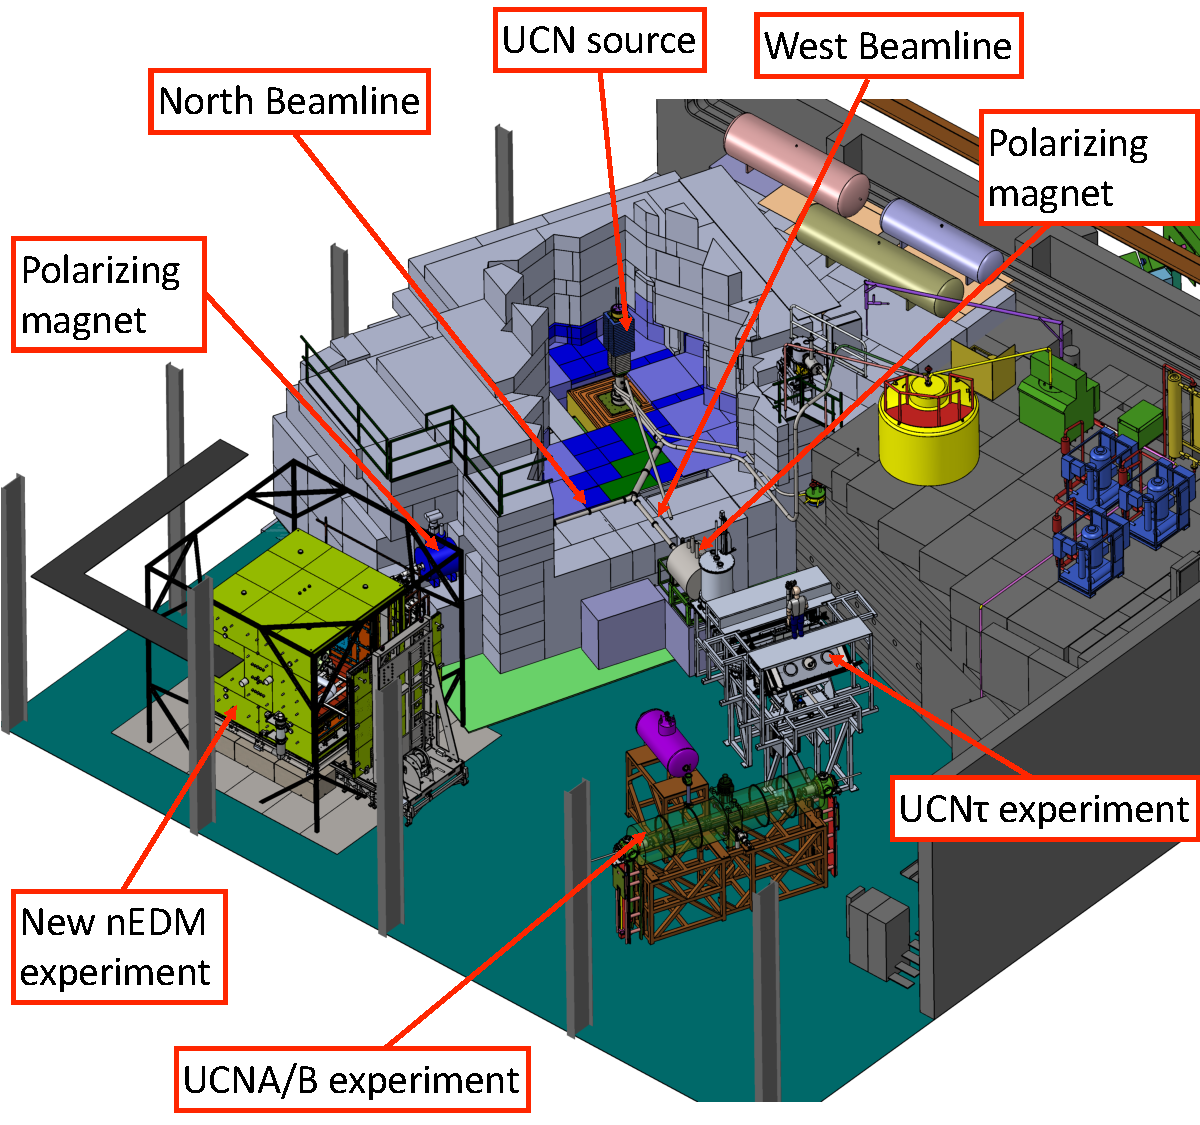
\includegraphics[width=0.6 \textwidth]{AreaB_v3.pdf}
    \caption[Schematic of the experimental area at the LANL UCN facility.]
    {Schematic of the experimental area at the LANL UCN facility. Rendering by Chris O'Shaughnessy.}
    \label{fig:AreaB_schematic}
\end{figure}

\begin{figure}
    \centering
    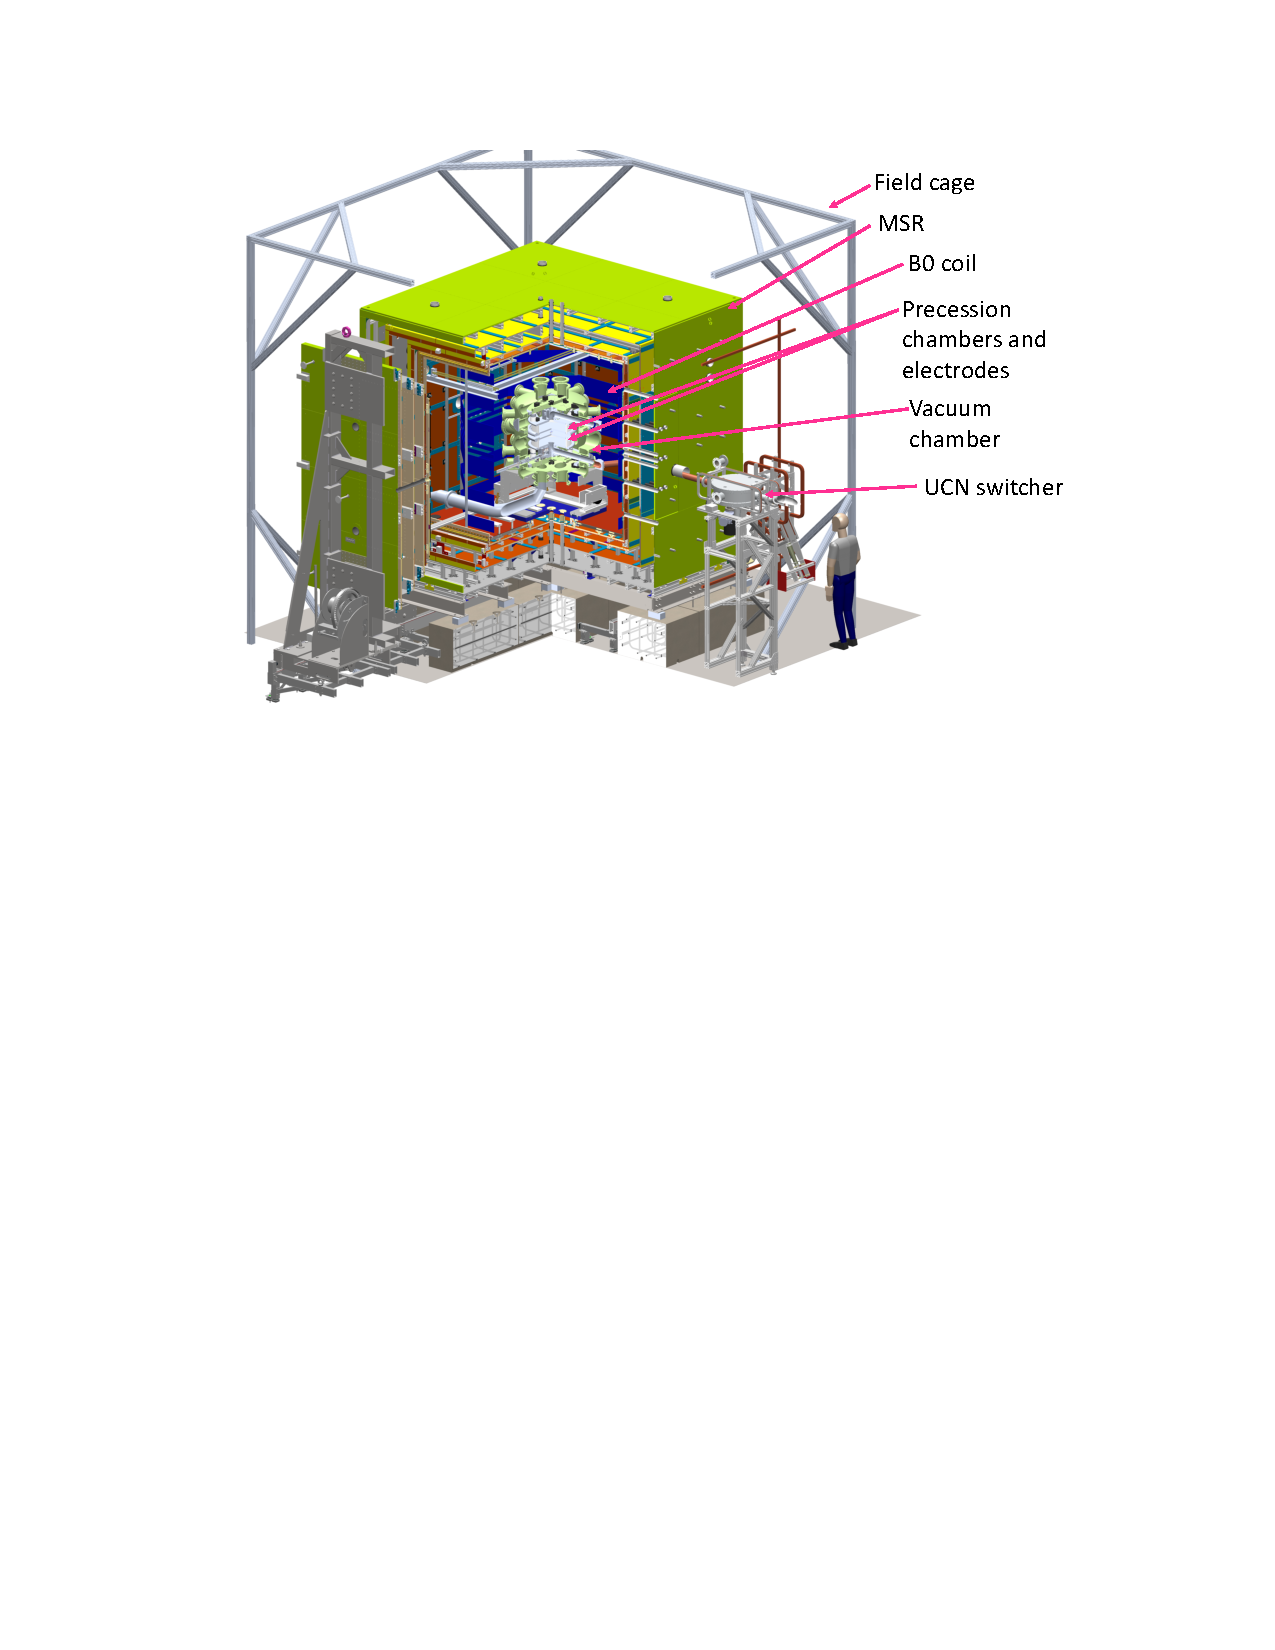
\includegraphics[width=0.9\textwidth]{figures/envisioned_lanl_nedm.pdf}
    \caption[Model of the LANL nEDM experiment.]
    {Model of the LANL nEDM experiment. Rendering by Chris O'Shaughnessy.}
    \label{fig:envisioned_lanl_nedm}
\end{figure}

%%%%%%%%%%%%%%%%%%%%%%%%%%%%%%%%%%%%%%%%%

\section{Statistical uncertainty}\label{sec:figure_of_merit}

%%%%%%%%%%%%%%%%%%%%%%%%%%%%%%%%%%%%%%%%%

Equation~(\ref{eq:ramsey_fringe_modulation_N_cos}) gives the number of neutrons counted in a single Ramsey sequence as
%
\begin{gather}
    N(\Delta \omega) = N_0 \left( 1 - \gls*{alpha} \cos \,\Delta \omega \, \gls*{T_fp} \right)/2 \nonumber
\end{gather}
%
where \gls*{alpha} is the spin contrast of a Ramsey fringe, defined by Eq.~(\ref{eq:alpha}), $\gls*{T_fp}$ is the free precession period of the Ramsey method, and $\Delta\omega=\omega-\omega_0$, where $\omega$ is the applied RF frequency and $\omega_0$ is the Larmor precession frequency.

To maximize sensitivity to small shifts in the resonant frequency, we examine where the slope of the central fringe is largest
%
\begin{gather}
    \frac{\partial N(\Delta \omega)}{\partial \, \Delta \omega} = N_0 \frac{\alpha}{2} \gls*{T_fp} \sin \, \Delta \omega \, \gls*{T_fp} \label{eq:slope_ramsey}
\end{gather}
%
The error of $\Delta \omega$ is given by
%
\begin{gather}
    \sigma(\Delta \omega) = \frac{\partial \, \Delta \omega}{\partial N(\Delta \omega)}\delta N(\Delta \omega) = \frac{\partial \, \Delta \omega}{\partial N(\Delta \omega)} \sqrt{N_0}
    \label{eq:sigma_delta_omega}
\end{gather}
%
Using Eq.~(\ref{eq:slope_ramsey}) where $\Delta \omega \, \gls*{T_fp} = \pi/2$ (for the largest slope), Eq.~(\ref{eq:sigma_delta_omega}) becomes
%
\begin{gather}
    \sigma(\Delta \omega) = \frac{2}{\gls*{alpha} \gls*{T_fp} \sqrt{N_0}}
\end{gather}
%
From reversal of the electric field, Eq.~(\ref{eq:delta_omega_dipole_relation}), we remove the dependence on $\Delta\omega$ to obtain
%
\begin{gather}
    \sigma_{\gls*{d_n}} = \frac{\hbar}{2\gls*{alpha} E \gls*{T_fp} \sqrt{N_0}}\label{eq:figure_of_merit}
\end{gather}
%
This is the figure of merit for an nEDM experiment using the Ramsey method. \gls{hbar} is Planck’s constant, $N_0$ (hereon notated as simply $N$) is the number of detected UCN, \gls{alpha} (Eq.~(\ref{eq:alpha})) is the spin contrast of the Ramsey fringe, and $E$ is the strength of the applied electric field. 

%%%%%%%%%%%%%%%%%%%%%%%%%%%%%%%%%%%%%%%%%

\subsection
{
    \texorpdfstring{Statistical Uncertainty of the \acrshort{lanl} \acrshort{nedm} experiment}
                    {Statistical Uncertainty of the LANL nEDM experiment}\label{sec:lanl_nedm_uncertainty}
}

%%%%%%%%%%%%%%%%%%%%%%%%%%%%%%%%%%%%%%%%%

The nominal run parameters for the LANL nEDM relevant to the estimate of uncertainty are $\gls*{T_fp}=180\text{ s and } E=12\text{ kV/cm}$. As will be shown in Chap.~\ref{chap:north_beamline_paper}, we have measured in excess of $N\simeq 40\,000\text{ UCN}$ in a prototype cell. We let $\gls*{alpha}=0.8$, as was achieved in Ref.~\cite{ABE20}.

Using Eq.~(\ref{eq:figure_of_merit}), the uncertainty per cell per run is $\num{9.5e-25}\,e\,\text{cm}$. For a full day of measurements (assuming a \qty{300}{\s} duty cycle with two precession cells), we have $N_\text{day}=2\times40\,000\times86\,400\text{ (seconds in a day)}/300$ and $\sigma_{\gls*{d_n}}=\num{3.96e-26}\,e\,\text{cm}$. A year of continuous running gives $N_\text{year}=365\times N_\text{day}$ and $\sigma_{\gls*{d_n}}=\num{2.07e-27}\,e\,\text{cm}$. At a 90\% confidence level, the uncertainty is multiplied by an additional factor of $1.6$, giving
%
\begin{gather}
    \sigma_{\gls*{d_n}}=\num{3.32e-27}e\,\text{cm (90\% \acrshort{cl})}
\end{gather}
%
The accelerator production schedule at LANL has about 7 months of accelerator operation from June through December with regular outages due to ion source recycling and other reasons. With an assumed data taking efficiency of 50\% for experiment down time, calibration and systematic studies, this uncertainty would be reached in 5 calendar years.



%%%%%%%%%%%%%%%%%%%%%%%%%%%%%%%%%%%%%%%%%

\section
{
    \texorpdfstring{UCN production at \acrshort{lanl}}
                   {UCN production at LANL}
}\label{sec:lanl_ucn_source}

%%%%%%%%%%%%%%%%%%%%%%%%%%%%%%%%%%%%%%%%%

\begin{figure}
    \centering
    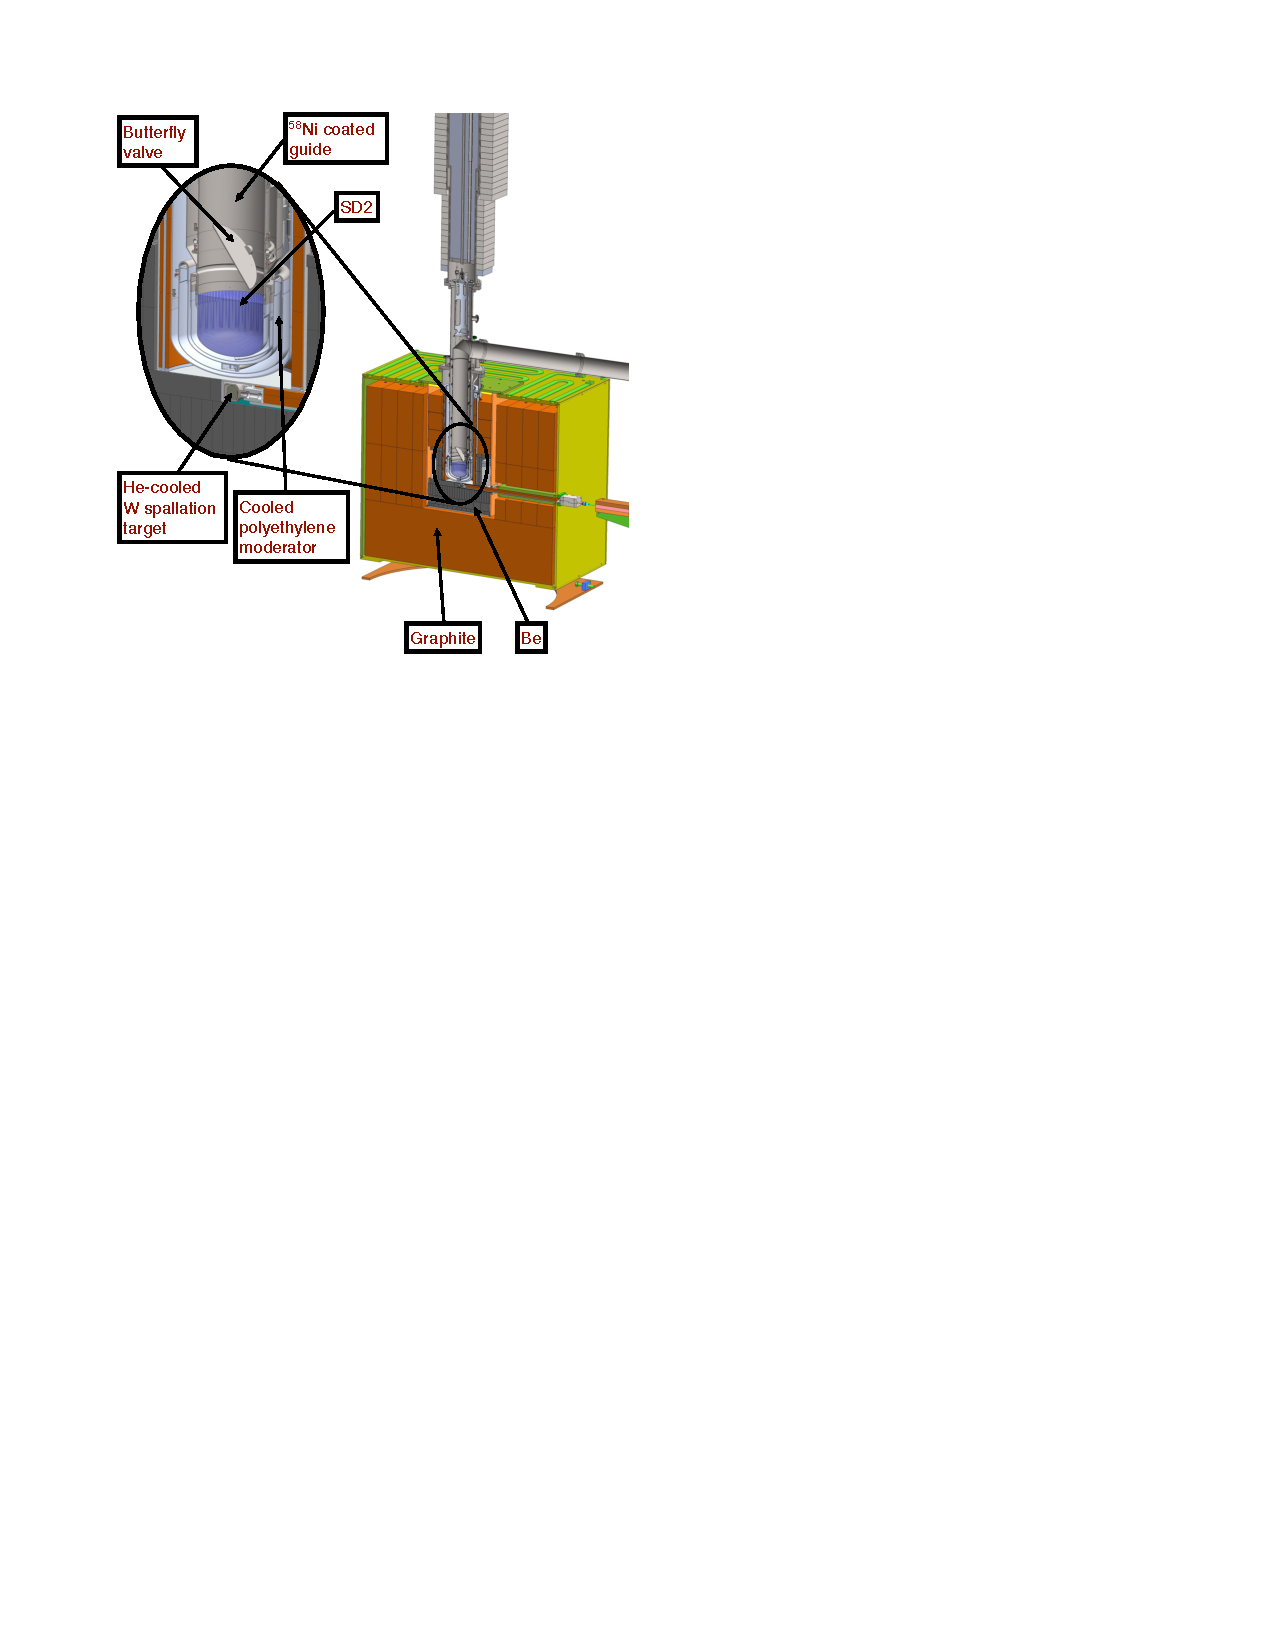
\includegraphics[height=4in]{figures/lanl_ucn_source.pdf}
    \caption[Cutaway view of the LANL UCN source]
    {Cutaway view of the LANL UCN source. Image adapted from Ref.~\cite{ito_performance_2018}}
    \label{fig:lanl_ucn_source}
\end{figure}

At LANL, neutrons are produced by a pulsed \qty{800}{M\eV} proton beam incident on a tungsten target. The spallation neutrons are moderated by room temperature beryllium and graphite, then converted to cold neutrons by cold polyethylene bead moderators, and finally become UCN by downscattering within an SD$_2$ crystal~\cite{saunders_performance_2013}.

As in Fig.~\ref{fig:lanl_ucn_source}, UCN leaving the SD$_2$ crystal are directed upwards along a \qty{1}{\meter} vertical guide coated in $\ce{^{58}Ni}$, to account for a Snell's law \qty{100}{\nano\eV} boost (Sec.~\ref{sec:ucn_reflection_transmission}). The UCN are then transported \qty{6}{\meter} along a horizontal NiP coated stainless steel guide to the exit of the biological shield~\cite{ito_performance_2018}.

A butterfly valve near the bottom of the vertical guide reduces the probability of UCN returning to the SD$_2$, in which \ucn has a short lifetime. The valve is open while proton beam pulses are delivered to the spallation target and closed otherwise. The proton current from the accelerator is delivered in packets of 10 pulses, of pulse width \qty{625}{\micro\s} at \qty{20}{\hertz}, with a gap between packets of \qty{5}{\s}. The average current delivered to the target is $\sim\qty{9}{\micro A}$.

In a 2017 source upgrade, the cryogenic insert, which housed the SD$_2$ converter as well as the cold neutron moderator, was replaced with an improved design. The upgrade produced a factor of four increase in UCN density. UCN density measured at the exit of the biological shield was $\qty{184(32)}{UCN\per \cm^3}$, and the polarized UCN density stored in an external cell was $\qty{39(7)}{UCN\per \cm^3}$~\cite{ito_performance_2018}.

With the upgrade, a new UCN beamline (called the North Beamline) was constructed for the new nEDM experiment (Fig.~\ref{fig:AreaB_schematic}). Measurements and analysis characterizing the performance of the North Beamline are presented in Chap.~\ref{chap:north_beamline_paper}.


%%%%%%%%%%%%%%%%%%%%%%%%%%%%%%%%%%%%%%%%%

\section
{
    Magnetic field uniformity and stability requirements\label{sec:magnetic_field_req}
}

%%%%%%%%%%%%%%%%%%%%%%%%%%%%%%%%%%%%%%%%%

Magnetic shielding and magnetic uniformity specifications for the LANL nEDM were based on two main requirements. The first requirement was the suppression of $v\times E$ motional effects, the largest of which is the geometric phase (Sec.~\ref{sec:v_cross_E}). A $\sim\qty{1}{pT\per cm}$ (or $\qty{0.1}{nT\per m}$) gradient creates a geometric phase false EDM in UCN of magnitude $|d_\text{false}|\sim 10^{-28}\,e\text{ cm}$~\cite{lamoreaux_geometric_phase_2005}, with the effect amplified in the faster moving \hg comagnetometer atoms (Sec.~\ref{sec:199hg_comag}). The second requirement was sufficiently long spin relaxation times $T_1$ and $T_2$ (Sec.~\ref{sec:spin_relaxation}) for the completion of a Ramsey sequence. Table~\ref{tb:lanl_magnetic_design} summarizes the design specifications for the magnetic environment of the LANL nEDM.

Stability requirements are based on the reasoning that noise from magnetic field fluctuation must be smaller than the counting statistics for a single measurement cycle~\cite{baker_apparatus_2014}
%
\begin{gather}
    \left| \frac{dB_0}{dt}\right| \frac{\gls*{gamma_n}\gls*{T_fp}}{2\pi} < \frac{1}{2\pi\gls*{alpha}\gls*{T_fp}\sqrt{N}} \label{eq:magnetic_stability}
\end{gather}
%
The constraint imposed by Eq.~(\ref{eq:magnetic_stability}) is harsher than necessary because the Ramsey method is relatively insensitive to fluctuations on time scales $\ll \gls*{T_fp}$ and because the \hg comagnetometer provides corrections. However, the nEDM measurement performed by Baker et al.~\cite{BAK06} had a comparable magnetic environment to the LANL nEDM and satisfied $|dB_0/dt|<\qty{8}{fT\per s}$ for most measurement cycles~\cite{baker_apparatus_2014}.

Homogeneity requirements from $T_2$ are derived by estimating the phase difference accumulated during the free precession period by \ucn with divergent paths in a field gradient. The absolute homogeneity requirement is ~\cite{baker_apparatus_2014}
%
\begin{gather}
    \Delta B_0 < \frac{1}{\gls*{gamma_n}}\sqrt{\frac{\overline{v}}{\overline{l}_0 \gls*{T_fp}}}
\end{gather}
%
where $\overline{l}_0$ is the average distance between wall collisions and $\overline{v}$ is the average \ucn velocity. The relative homogeneity is expressed as $\Delta B_0/B_0$.

\begin{table}
\renewcommand*{\arraystretch}{2} % increase vertical spacing just for this table
\centering
\caption{Design requirements of the magnetic environment for the LANL nEDM experiment and physical considerations from which they arise}\label{tb:lanl_magnetic_design}
\begin{tabular}{
    lll
}
\toprule
Parameter		& Specification				& Considerations	\\
\midrule
Field gradient $(\partial B/\partial z)/B_0$	& $10^{-4}/\text{cm or } <\qty{10}{nT\per m}$ & $T_2$ relaxation time $\sim\qty{1000}{s}$\\
Field gradient  & $3\times 10^{-6}/\text{cm or }<\qty{0.3}{nT\per m}$ & $|d_\text{false}|<10^{-27}\,e\text{ cm}$ \\
Residual field & $<\qty{5}{nT}$ & $\vv{E}$ and $\vv{B}$ alignment $\theta_{EB}<\qty{0.5}{\degree}$ \\
Shielding factor & $>10^4$ for $f>\qty{0.01}{Hz}$ & Temporal drift \\
\makecell[l]{Difference in $\langle B_0 \rangle$\\between precession cells} & $<\qty{10}{pT}$ & \makecell[l]{Flip \ucn with the same $\pi/2$\\pulse after \gls*{T_fp}} \\
\bottomrule
\end{tabular}
\end{table}

%%%%%%%%%%%%%%%%%%%%%%%%%%%%%%%%%%%%%%%%%

\subsection
{
    \texorpdfstring{\hg Comagnetometer}
                    {199Hg Comagnetometer}\label{sec:199hg_comag}
}

%%%%%%%%%%%%%%%%%%%%%%%%%%%%%%%%%%%%%%%%%

A comagnetometer is a polarized population of atoms occupying the same precession cell as \ucn. It provides information regarding the volume averaged magnetic field $\langle B_0 \rangle$ over the course of the free precession period. Comagnetometers must have a low \ucn absorption cross section, sufficiently long spin polarization lifetimes, a small EDM that does not mask the nEDM, and compatability with \ucn-friendly surfaces~\cite{golubUCN}.

\hg offers several advantages: it can be optically pumped, the precession frequency can be extracted optically, and has been used successfully in previous nEDM measurements (Refs.~\cite{BAK06, ABE20}). However, it suffers from the drawback of sensitivity to high voltage (\acrshort*{hv}), which can reduce the spin relaxation time. This limits the magnitude of $E$ that may be applied across the electrodes. (Depolarization-inducing hydrogen is released in micro-discharges with the application of high voltage, which must be cleaned by flowing oxygen through the precession cell~\cite{baker_apparatus_2014}.)

Due to its higher velocity, \hg experiences a larger geometric phase shift and has a slightly higher center of mass compared to \ucn in the precession cell. As per Ref.~\cite{pendlebury_revised_2015} the geometric phase false EDM contribution from \hg is $\sim 50$ times larger than the contribution from \ucn. 

One method to account for the geometric phase effect was utilized by Baker et al.~\cite{BAK06}. In the absence of the geometric phase effect, the measured ratio $|\omega_\text{n}/\omega_\text{Hg}|$ may be compared to the expected value of $|\gls{gamma_n}/\gamma_\text{Hg}|$. However, in reality $\omega_\text{Hg}$ contains a contribution from the geometric phase effect. To account for the effect, the measurement is repeated for different applied magnetic field gradients. The ratio $|\omega_\text{n}/\omega_\text{Hg}|/|\gls{gamma_n}/\gamma_\text{Hg}|$ is then extrapolated to the limit where the field gradient is zero and the Hg geometric phase vanishes.

The LANL nEDM has acquired a \qty{254}{\nano\meter} Toptica laser for the development of the comagnetometer system, with the intention of adding external \hg cells to be used for magnetic gradient readout. The \hg cells will be vertically aligned and placed between the two precession cells (Sec.~\ref{sec:precession_cells}).

%%%%%%%%%%%%%%%%%%%%%%%%%%%%%%%%%%%%%%%%%

\subsection{External magnetometry}\label{sec:external_magnetometry}

%%%%%%%%%%%%%%%%%%%%%%%%%%%%%%%%%%%%%%%%%

An array of external monitors will be used to measure magnetic fields and gradients in close proximity to the precession cells. The LANL nEDM and industry partner Twinleaf are working to develop Cs magnetometers with sufficient stability and sensitivity for application to a nEDM measurement. The required sensitivity is for the magnetometer to measure changes in magnetic field better than \qty{70}{fT} per \qty{180}{s} fill of the cell, and to be stable to \qty{50}{fT} over \qty{480}{s}. Two prototypes have been built and instrumented by Twinleaf, and are being optimized by LANL nEDM collaboration members.


%%%%%%%%%%%%%%%%%%%%%%%%%%%%%%%%%%%%%%%%%

\section
{
    \texorpdfstring{$v\times E$ motional effect systematics}
                    {v x E motional effect systematics}\label{sec:v_cross_E}
}

%%%%%%%%%%%%%%%%%%%%%%%%%%%%%%%%%%%%%%%%%

A particle with velocity $\vv{v}$ moving in fields $\vv{E}$ and $\vv{B}_0$ sees in its rest frame a field $\vv{B}'$ given by
%
\begin{align}
    \vv{B}' &= \vv{B}_0+\vv{B}_{v\times E} \\
            &= \vv{B}_0-\gls{lorentz}\frac{\vv{v}\times\vv{E}}{c^2}
\end{align}
%
where the Lorentz factor $\gls*{lorentz}=\glsvalue*{lorentz}\approx 1$ for \ucn and cold neutron velocities. When compounded with other factors described in this section, this gives rise to false EDM signals.

Again borrowing the form of Eq.~(\ref{eq:delta_omega_dipole_relation}), we see that $E$-odd terms that shift precession frequency create a false EDM because they do not disappear upon reversal of the $E$ field.
%
\begin{gather}
    d_\text{false}=\frac{\hbar}{4E}(\Delta\omega(E)-\Delta\omega(-E))
\end{gather}

\subsection*{
    \texorpdfstring{Nonparallel $E$ and $B$ fields}
                    {Nonparallel E and B fields}
}

We first examine the false EDM from misalignment of $E$ and $B$ fields in combination with the $v\times E$ effect. Let $\theta_{EB}$ be the angle between $\vv{E}$ and $\vv{B}_0$ in the plane perpendicular to $\vv{v}$. The magnetic field in the particle rest frame is then~\cite{lamoreaux_experimental_2009}
%
\begin{align}
    B^{\prime^2} &= B^{\prime^2}_z + B^{\prime^2}_{xy} \\
    &= (B_0 +  B_{v\times E}\sin\theta_{EB})^2 + ( B_{v\times E}\cos\theta_{EB})^2 \\
    &= B_0^2\left(1 + 2\frac{ B_{v\times E}}{B_0}\sin\theta_{EB} + \frac{ B_{v\times E}^2}{B_0^2}\right)\\
    &\approx B_0 + \theta_{EB} B_{v\times E} + \frac{B_{v\times E}^2}{2B_0}
\end{align}
%
where in the last line we use $B_{v\times E} \ll B_0$ and $\sin\theta\approx\theta$. Keeping only $E$-odd terms, the frequency shift from the false EDM is therefore
%
\begin{align}
    \Delta\omega_\text{false} &\approx -\gls{gamma_n}\left( \theta_{EB} B_{v\times E} + \frac{B_{v\times E}^2}{2B_0} \right) \label{eq:vxE_motional_shift}\\
    &\approx -\gls{gamma_n} \frac{\theta_{EB}v}{c}E 
\end{align}
%
For cold neutron beam nEDM experiments (Sec.~\ref{sec:history_nedm}) this systematic was quite substantial. For reference, the uncertainty of the most accurate beam nEDM experiment to date \cite{dress_nedm_1977} constrained $\theta_{EB}$ to $<\qty{1.1e-4}{rad}$, but was still limited by an uncertainty of $\sim 10^{-24}\,e\text{ cm}$. (To reduce the $v\times E$ effect, the experiment was even built on a naval gun turret mount to enable the reversal of $\vv{v}$ through the apparatus!) 

In contrast, nEDM experiments using stored \ucn gain the benefit of $\langle v \rangle =0$ for the neutron population. Assuming there is no persistent overall motion of the \ucn caused by the storage geometry, filling procedure, etc., the systematic effects of nonparallel $E$ and $B$ fields are negligible at current sensitivities. Demands on field alignment are particularly relaxed if \ucn reflections off the internal surface of the precession cell are sufficiently nonspecular~\cite{pendlebury_revised_2015}.

\subsection*{Motional effect quadratic term}

The right hand side of Eq.~(\ref{eq:vxE_motional_shift}) also contains a term quadratic in $E$
%
\begin{gather}
    \Delta\omega_\text{false} = -\gls{gamma_n} \frac{v^2}{2c^2}\frac{E^2}{B_0} 
\end{gather}
%
where a change in $|E|$ between $\vv{B}_0\uparrow\uparrow\vv{E}$ and $\vv{B}_0\uparrow\downarrow\vv{E}$ modes produces a correlated frequency shift. As discussed in Ref.~\cite{lamoreaux_experimental_2009}, even if $\langle v \rangle=0$ for stored particles, the quadratric term does not necessarily go to zero due to the $v^2$ factor. At current sensitivities the false EDM contribution from the quadratic term is still negligible.

\subsection*{Geometric phase}

Mangetic field components transverse to $\vv{B}_0$ due to field inhomogeneity in combination with the $v\times E$ effect gives rise to the geometric phase effect, a large false EDM signal at current sensitivities. 

Pendlebury et al.~\cite{pendlebury_geometric-phase-induced_2004} considered the often-cited example of a  magnetic ``barrel'' gradient with cylindrical symmetry and particles in roughly circular orbits about a precession cell.
%
\begin{gather}
    B_r(r)=\frac{r}{2}\frac{\partial B_z}{\partial z}
\end{gather}
%
The gradient and $v\times E$ effect produce a rotating field in the rest frame of the particle, resulting in a variant of the Bloch-Siegert shift (Sec.~\ref{sec:bloch-siegert}). The magnitude of the geometric phase shift is dependent on the ratio of the orbital-trajectory frequency of a particle to its Larmor precession frequency. Slow moving \ucn (adiabatic) see a shift given by~\cite{pendlebury_geometric-phase-induced_2004, afach_measurement_2015}
%
\begin{gather}
    \Delta\omega_\text{false} = \frac{v^2_{xy}}{2 B_0^2 c^2}\frac{\partial B_z}{\partial z}E
\end{gather}
%
and the faster \hg comagetometer atoms (nonadiabatic) see
%
\begin{gather}
    \Delta\omega_\text{false} = \frac{\gamma^2 D^2}{16  c^2}\frac{\partial B_z}{\partial z}E
\end{gather}
%
where $v_{xy}$ is the average transverse particle velocity, $\gamma$ is the gyromagnetic ratio of the particle, and $D$ is the diameter of the precession cell. 

Of course, particles are not limited to strictly circular orbits about a cylindrical precession cell. In addition to using Monte Carlos simulations (such as in Ref.~\cite{pignol_magic_2019}), more general expressions for geometric phase have been derived. References~\cite{pignol_geometric_phase_2012, pignol_geometric_phase_2015} use a perturbative treatment of transverse field inhomogeneities in the nonadiabatic limit to obtain
%
\begin{gather}
    \Delta\omega_\text{false} = \frac{\gamma^2}{c^2}\langle xB_x + yB_y \rangle E
\end{gather}
%
where $\langle ... \rangle$ denotes a volume average over a precession cell of arbitrary geometry.

A formalism of geometric phase shift in terms of velocity autocorrelation functions can be found in Refs.~\cite{lamoreaux_geometric_phase_2005, barabanov_geometric_phase_2006, swank_geometric_phase_2009}.
%
\begin{align}
    \Delta\omega_\text{false} &= -\frac{\gamma^2 E}{2c^2}\left( \frac{\partial B_y}{\partial y} S_y(\omega_0) + \frac{\partial B_z}{\partial z} S_z(\omega_0) \right) \\
    S_i(\omega_0) &= 2\int_{-\infty}^{\infty} \frac{\Psi_i(\omega)}{(\omega_0^2 - \omega^2)}d\omega \\
    \Psi_i(x) &= \langle v_i(t)v_i(t-x) \rangle = \int_{-\infty}^{\infty}\cos (\omega x) \Psi_i (\omega) d\omega
\end{align}


%%%%%%%%%%%%%%%%%%%%%%%%%%%%%%%%%%%%%%%%%

\section{Additional sources of false EDMs}

%%%%%%%%%%%%%%%%%%%%%%%%%%%%%%%%%%%%%%%%%

\subsection*{Leakage current and other electric forces}

With the application of \acrshort{hv} through the electrodes, small leakage currents will flow through the insulating cell wall (Sec.~\ref{sec:precession_cells}). A current with a net azimuthal component from a helical path creates a vertical magnetic field correlated with the direction of the electric field, a false EDM signal. Reference~\cite{baker_apparatus_2014} estimates this false EDM magnitude to be
%
\begin{gather}
    | d_\text{false} | = 0.1\frac{\gls*{mu_n}}{E}\frac{\mu_0 I}{2r}f \sim \num{1e-28}\,e\text{ cm}
\end{gather}
%
where $r$ is insulator radius and $f$ is the fraction of a complete loop about the insulator that the current $I$ takes. The factor of $0.1$ is present because the \hg comagnetometer is approximated to compensate for the leakage current frequency shift at a 90\% level. The nEDM measurement performed without a comagnetometer in Ref.~\cite{serebrov_leakage_current_2015} uses a broad range of possible leakage current paths and simulated UCNs to estimate a false nEDM $<10^{-26}\,e\text{ cm}$.

See Refs.~\cite{baker_apparatus_2014, pendlebury_revised_2015} for examination of higher order effects caused by high voltage, such as sparking or induced RF fields from ripples. 

\subsection*{Earth's rotation}

The laboratory frame is affected by Earth's rotation, and the rotation of the Earth adds to or subtracts from the measured \ucn precession frequency, depending on the relative direction of Earth's rotation and the precession. The simplest example is an experiment taking place at the North pole with vertical $\vv{E}$ and $\vv{B}$ fields, which directly follows the rotation of the Earth and sees a corresponding shift in measured precession frequency.

This shift in Larmor precession at the location of the LANL nEDM experiment is approximately \qty{10}{\micro Hz}. An additional complication is that the gyromagnetic ratio for neutrons is negative, but the positive for \hg.  For nEDM measurements that use the measured ratio $|\omega_\text{n}/\omega_\text{Hg}|$ (Sec.~\ref{sec:199hg_comag}), the Earth's rotation shifts the ratio value down (up) by $\sim\qty{1}{ppm}$ when $\vv{B}_0$ is upwards (downwards). See Refs.~\cite{lamoreaux_earth_rotation_comment, baker_reply_to_lamoreaux, pendlebury_revised_2015}.

%%%%%%%%%%%%%%%%%%%%%%%%%%%%%%%%%%%%%%%%%

\section
{
    \texorpdfstring{Magnetically Shielded Room}
                    {Magnetically Shielded Room}\label{sec:MSR}
}

%%%%%%%%%%%%%%%%%%%%%%%%%%%%%%%%%%%%%%%%%

\begin{figure}
    \centering
    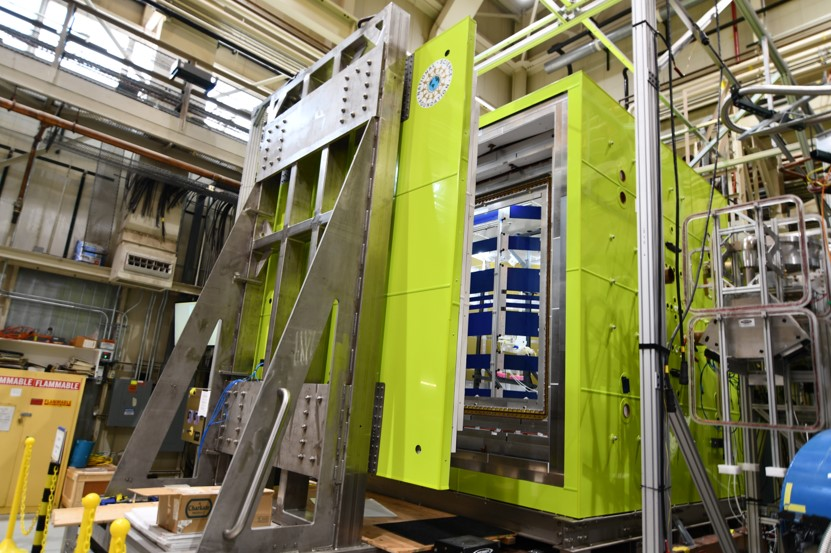
\includegraphics[width=0.9\textwidth]{figures/completed_msr.jpg}
    \caption
    {The LANL nEDM magnetically shielded room (Sec.~\ref{sec:MSR})}
    \label{fig:MSR}
\end{figure}

\begin{figure}
    \centering
    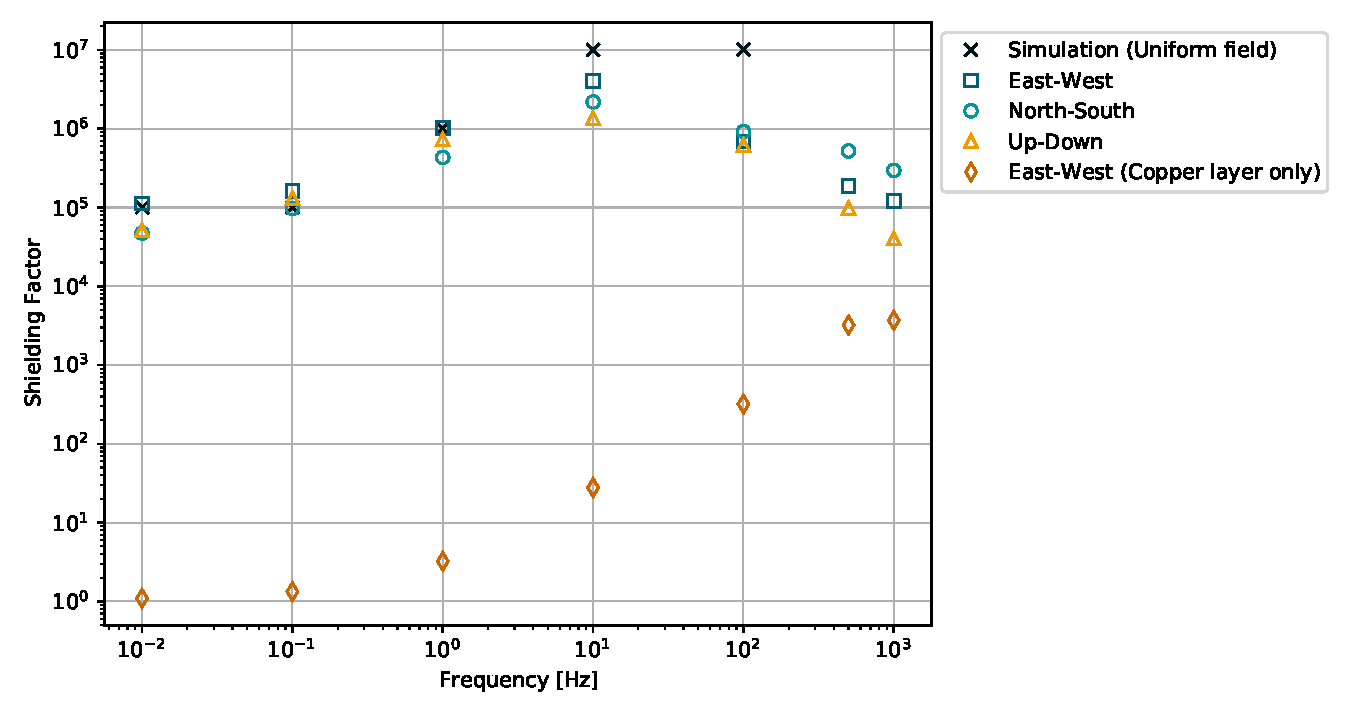
\includegraphics[width=0.9\textwidth]{figures/chupp_msr_data.pdf}
    \caption
    {Calculated shielding factors and measured values, corrected for the calculated geometrical factor, of the LANL nEDM MSR (Tab.~\ref{tb:lanl_msr_shielding_factor}). See Sec.~\ref{sec:MSR} for methodology.}
    \label{fig:MSR-shielding-factor}
% \end{figure}
    \vspace{\baselineskip}
% \begin{figure}
    \centering
    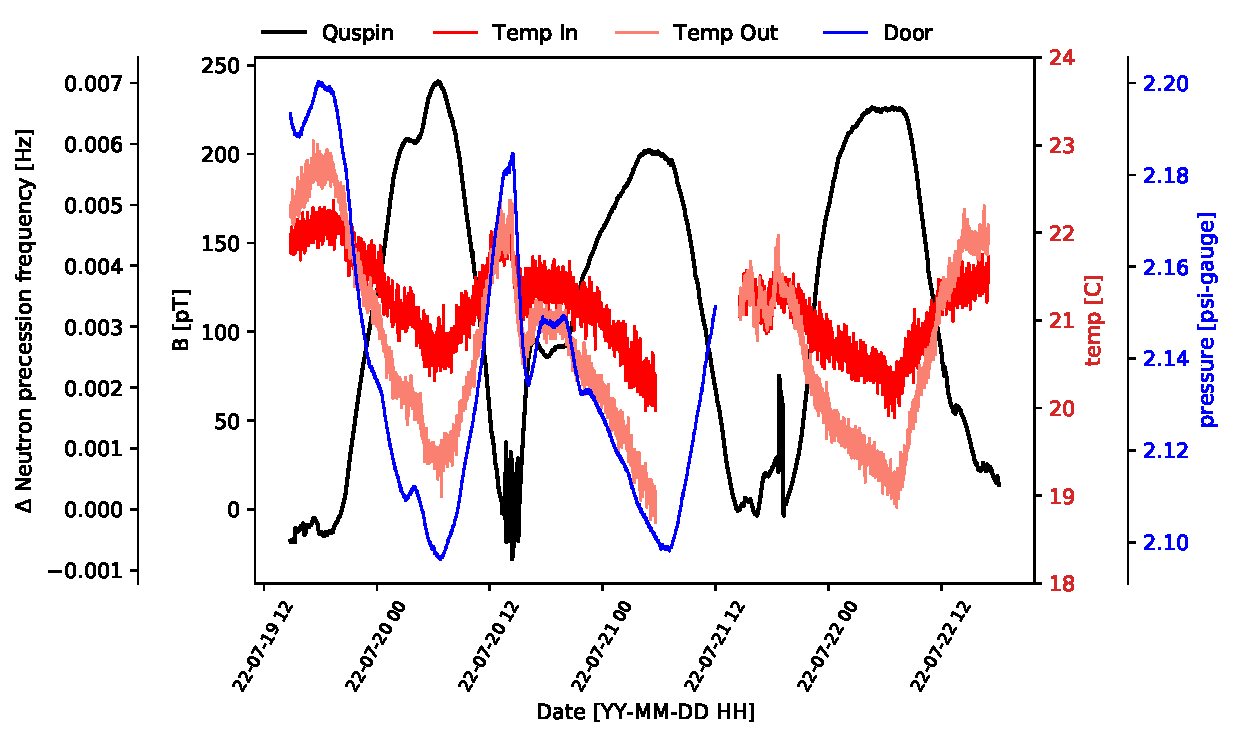
\includegraphics[width=0.9\textwidth]{figures/long_term_msr_measurements.pdf}
    \caption
    [A magnetic field measurement in the non-degaussed MSR over a 3 day period]
    {A magnetic field measurement in the non-degaussed MSR over a 3 day period from a QuSpin Zero-Field Magnetometer \legendbox{black} (sensitivity $<\qty{1}{pT\per\sqrt{Hz}}$ for 1--\qty{100}{\hertz}). Temperature is read by MLX90164 IR Temp sensors. The ``Temp Out'' sensor \legendbox{Salmon} is pointed at the outer cladding of the MSR, and the ``Temp In'' sensor \legendbox{red} is pointed through a beamline feedthrough at a PCB panel of the $B_0$ coil. A Honeywell 236PC100GW Wheatstone-bridge pressure sensor \legendbox{blue} monitors the pressure of air line feeding the door bladders. Additional discussion in Sec.~\ref{sec:MSR}.}
    \label{fig:MSR_long_term_measurements}
\end{figure}

At LANL, a large magnetically shielded room (\acrshort*{msr}) (Fig.~\ref{fig:MSR}) is used for the attenuation of ambient external background magnetic fields. It has an overall shielding factor of $10^5$ for fields at frequency \qty{0.01}{\hertz} and a residual field of $<\qty{0.5}{nT}$. The design of the MSR heavily draws from recent advancements of the technology~\cite{altarev_msr_1, altarev_msr_2, altarev_msr_3}, where the placement of degaussing coil locations in combination with a rectangular MSR geometry results in optimized performance.

The MSR consists of 4 Mumetal\textsuperscript{\textregistered} layers and one copper layer (Tab.~\ref{tb:lanl_msr_layers}). Mumetal\textsuperscript{\textregistered} is a magnetic shielding alloy ($\mu$-metal grade ASTM A753 Alloy 4, UNS N14080, 80NiFe) from the Magnetic Shield Corporation. The MSR utilizes a bolted construction to avoid welds that create magnetic domains. The frame of the MSR is aluminum, which supports the load of the layers without deflection, and a support structure underneath is made of stainless steel. A foundation that consists of high density aggregate precast blocks minimizes the transmission of ambient external vibrations. The edges of the MSR door are supported by air bladders. When the door is in the closed and locked position, the air bladders are pressurized to improve continuity of the $\mu$-metal.

For improved shielding performance, the ferromagnetic layers are degaussed periodically. Degaussing is done by applying an alternating field with large amplitude, which drives the material to saturation, and then slowly decreasing the amplitude to zero. Each $\mu$-metal layer contains multiple L-shaped coil sets, activated sequentially, for complete degaussing coverage (see Fig.~\ref{fig:degaussing-paper-cube} for the layout of coils on the innermost layer). An amplifier designed and built specifically for the LANL nEDM allows application of up to \qty{75}{A} of current for degaussing.

Residual magnetic fields in the degaussed \acrshort*{msr} were measured with a low noise 3-axis Bartington fluxgate probe (Tab.~\ref{tb:lanl_msr_dc_residuals}). The fluxgate was mounted on a fiberglass structure, and was inserted through the large neutron guide access tubes of the MSR. At each position, a \qty{10}{\second} measurement per fluxgate axis was taken in addition to a corresponding measurement where the fluxgate was rotated by \qty{180}{\degree}.

The absolute magnetic field values for an axis ($i=x,y,z$) were then calculated using the relations
%
\begin{align}
    B_{i,\text{ un-rotated}}&=\text{offset}+B_{i}\\
    B_{i,\text{ rotated}}&=\text{offset}-B_{i}\\
    \text{offset}&= (B_{i,\text{ un-rotated}} + B_{i,\text{ rotated}})/2
\end{align}
%
From the offset-corrected field values, the measured gradient upper limit was found to be $\qty{0.51}{nT\per m}$.

Shielding factor was determined by using the LANL field cage (Sec.~\ref{sec:field-cage}) to provide excitation signals. The resulting amplitude was measured with a fluxgate at the center of the field cage both before the start of MSR construction and after construction was completed. The measured shielding factor was calculated from the ratio of the two amplitudes. Excitation signals of amplitude \qty{1}{\micro\tesla} were used for frequencies \qty{0.01}{\hertz} and \qty{0.1}{\hertz}, \qty{10}{\micro\tesla} for \qty{1}{\hertz}, and \qty{30}{\micro\tesla} for 10--\qty{1000}{\hertz}. 

To account for the finite size of the excitation coil and the iron floor of the experimental area, finite-element physics simulations in COMSOL were used to obtain a relation between the measured shielding factor and a calculated shielding factor with an ideal infinitely sized coil. This scaling was performed because the proximity of the field cage coils to the outer MSR layer resulted in localized saturation of the $\mu$-metal, artificially lowering the shielding factor. Measured and calculated shielding factors are shown in Fig.~\ref{fig:MSR-shielding-factor} and Tab~\ref{tb:lanl_msr_shielding_factor}. 

In the latter half of 2022, issues with the electrical contacts at the door for the degaussing wires on the innermost MSR layer developed. This has delayed additional characterization of MSR performance. 

The magnetic field in the non-degaussed MSR is plotted in Fig.~\ref{fig:MSR_long_term_measurements}. A fluctuation of $\sim\qty{250}{pT}$ (a $\sim \qty{1e-3}{Hz}$ shift in neutron precession frequency) with the periodicity of approximately one day was observed, correlated with ambient temperature fluctuations. This temperature fluctuation influences both the behavior of the $\mu$-metal and the pressure of the air bladders in the door, potentially altering the quality of $\mu$-metal continuity. Measurements to determine the necessity of external temperature regulation are planned after the degaussing loops are fixed. 

\begin{table}
\centering
\caption{MSR layer composition}\label{tb:lanl_msr_layers}
\begin{tabular}{
    l
    c
    l
    S[table-format=1.2]
    c
    S[table-format=1.2]
    c
    S[table-format=1.2]
}
\toprule
Layer		& Thickness      & Material                        & \multicolumn{5}{c}{External side length}	\\
  &  {[mm]}    &  &  \multicolumn{5}{c}{$\text{[m}\times \text{ m}\times\text{ m]}$} \\
\midrule
1--outer	& 4  & Mumetal\textsuperscript{\textregistered}    & 3.5 & $\times$ & 3.5 & $\times$ & 3.5 \\
2	        & 3  & Mumetal\textsuperscript{\textregistered}    & 3.0 & $\times$ & 3.0 & $\times$ & 3.0 \\
3	        & 3  & Mumetal\textsuperscript{\textregistered}    & 2.6 & $\times$ & 2.6 & $\times$ & 2.6 \\
4	        & 8  & Copper                                      & 2.46 & $\times$ & 2.46 & $\times$ & 2.46 \\
5--inner	& 4  & Mumetal\textsuperscript{\textregistered}    & 2.39 & $\times$ & 2.39 & $\times$ & 2.39 \\
\bottomrule
\end{tabular}
% \end{table}
\vspace{\baselineskip}\vspace{\baselineskip}
% \begin{table}
% \centering
\caption{Residual DC fields in degaussed MSR. The measured gradient upper limit was found to be $\qty{0.51}{nT\per m}$}\label{tb:lanl_msr_dc_residuals}
\begin{tabular}{
    c
    S[table-format = 2.0]
    S[table-format = 2.0]
    S[table-format = 2.0]
    S[table-format = 1.2]
}
\toprule
Point		& $x$				& $y$				& $z$				& $|B|$	\\
{}    		& {(rel. to center)}	        & {[cm]}       & {[cm]}		& {[nT]} 		\\
\midrule
1			& -40	            & -39	            & 23		        & 0.64\\
2			& 0	                & -39	            & 23	        	& 0.51\\
3			& 40                & -39	            & 23		        & 0.45\\
4			& -40	            & 39        		& -23	            & 0.52\\
5			& 0                 & 39        	    & -23	            & 0.41\\
6			& 40                & 39                & -23	            & 0.93\\
\bottomrule
\end{tabular}

% \end{table}
\vspace{\baselineskip}\vspace{\baselineskip}
% \begin{table}
% \centering
\caption{MSR shielding factors, measured and calculated (as per Sec.~\ref{sec:MSR})}\label{tb:lanl_msr_shielding_factor}
\begin{tabular}{
    c
    S[exponent-mode = scientific, table-format = 1.2e1]
    S[exponent-mode = scientific, table-format = 1.2e1]
}
\toprule
{Frequency}		& {Shielding factor}			& {Shielding factor}\\
{[Hz]}	& {(Measured)}	& {(corrected for geometry)} \\
\midrule
0.01    & 2.82e4    & 1.55e5 \\
0.1     & 4.55e4    & 2.50e5 \\
1       & 1.05e5    & 1.05e5 \\
10      & 7.72e4    & 4.25e5 \\
100     & 1.16e4    & 4.64e5 \\
\bottomrule
\end{tabular}

\end{table}


\begin{figure}
    \centering
    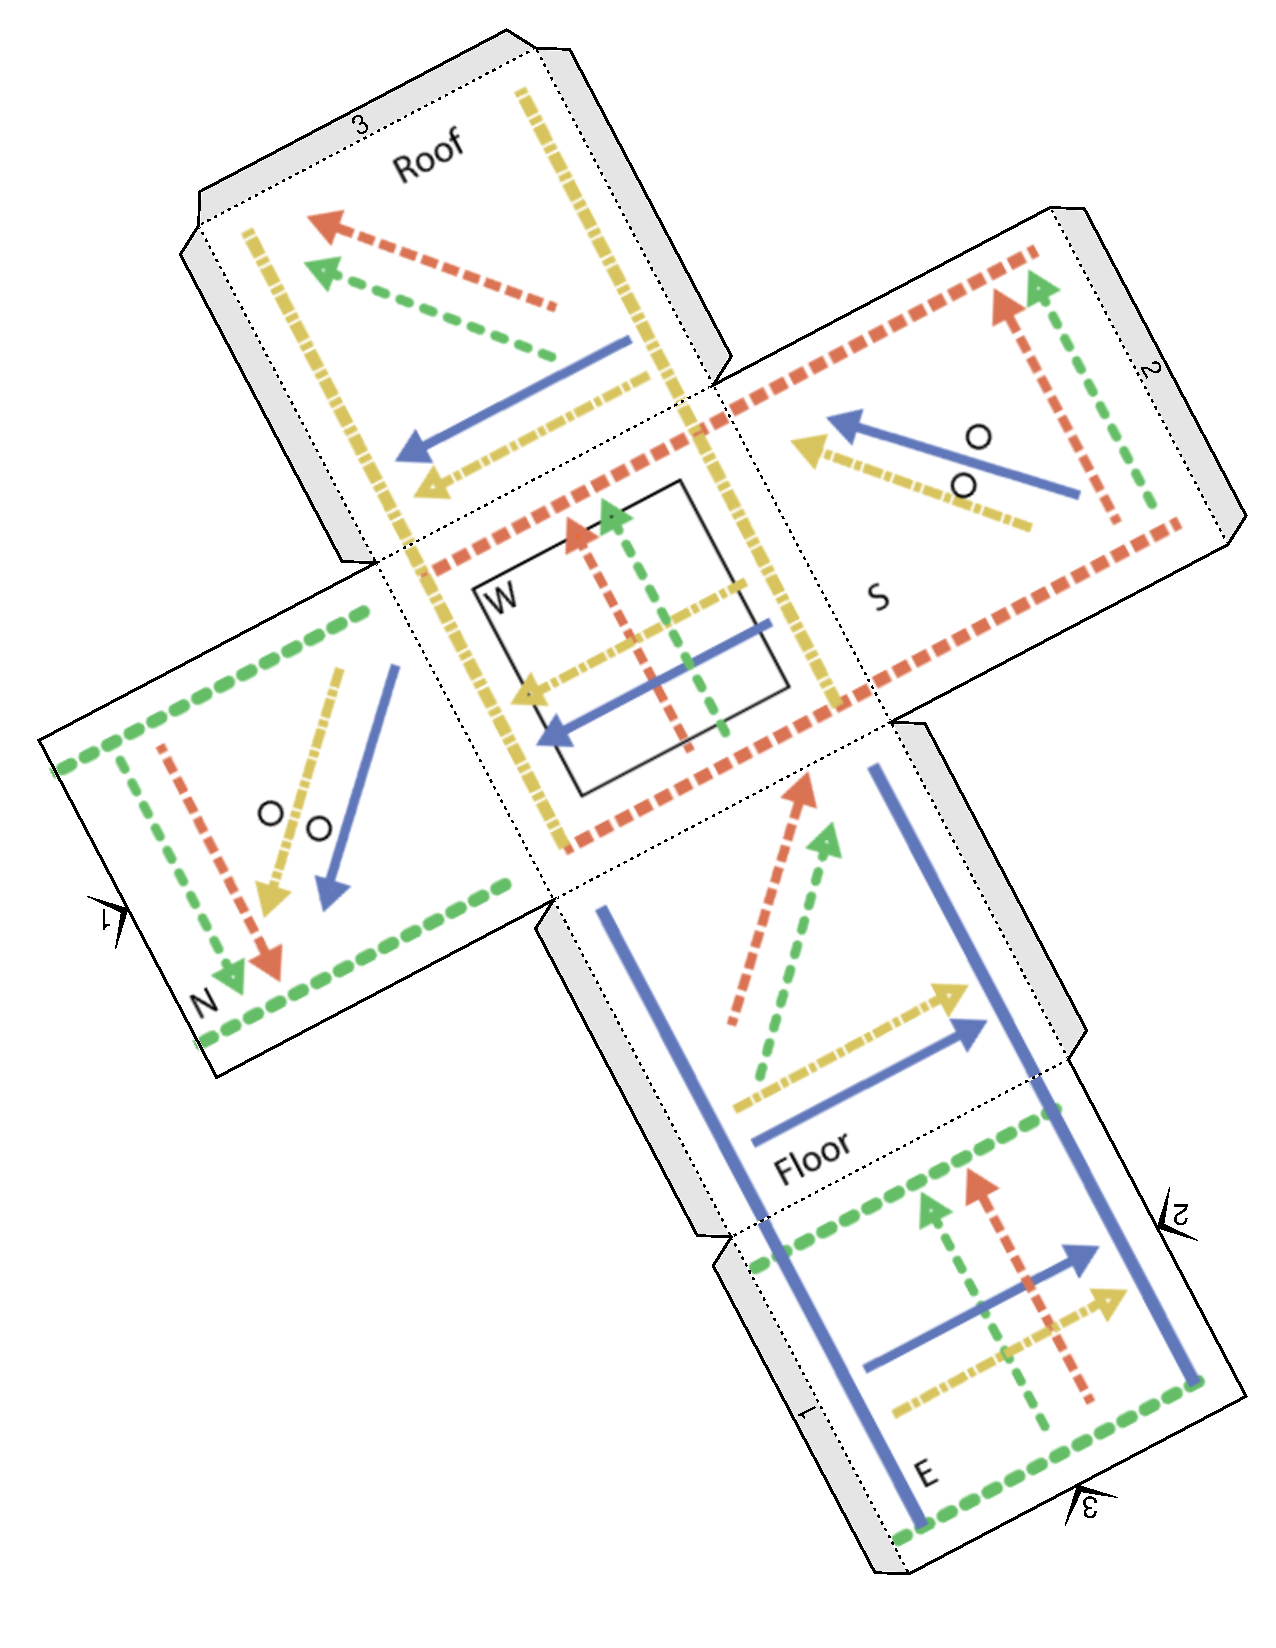
\includegraphics[width=\textwidth]{figures/L5-papercube.pdf}
    \caption
    [Simplified papercraft model of the four L-shaped degaussing coil sets on the innermost MSR layer and resulting flux contributions.]
    {Simplified papercraft model of the four L-shaped degaussing coil sets on the innermost MSR layer and resulting flux contributions. Figure courtesy of Austin Reid.}
    \label{fig:degaussing-paper-cube}
\end{figure}

%%%%%%%%%%%%%%%%%%%%%%%%%%%%%%%%%%%%%%%%%

\section{External field compensation coils}\label{sec:field-cage}

%%%%%%%%%%%%%%%%%%%%%%%%%%%%%%%%%%%%%%%%%

\begin{figure}
\centering
\begin{minipage}{.5\textwidth}
    \centering
    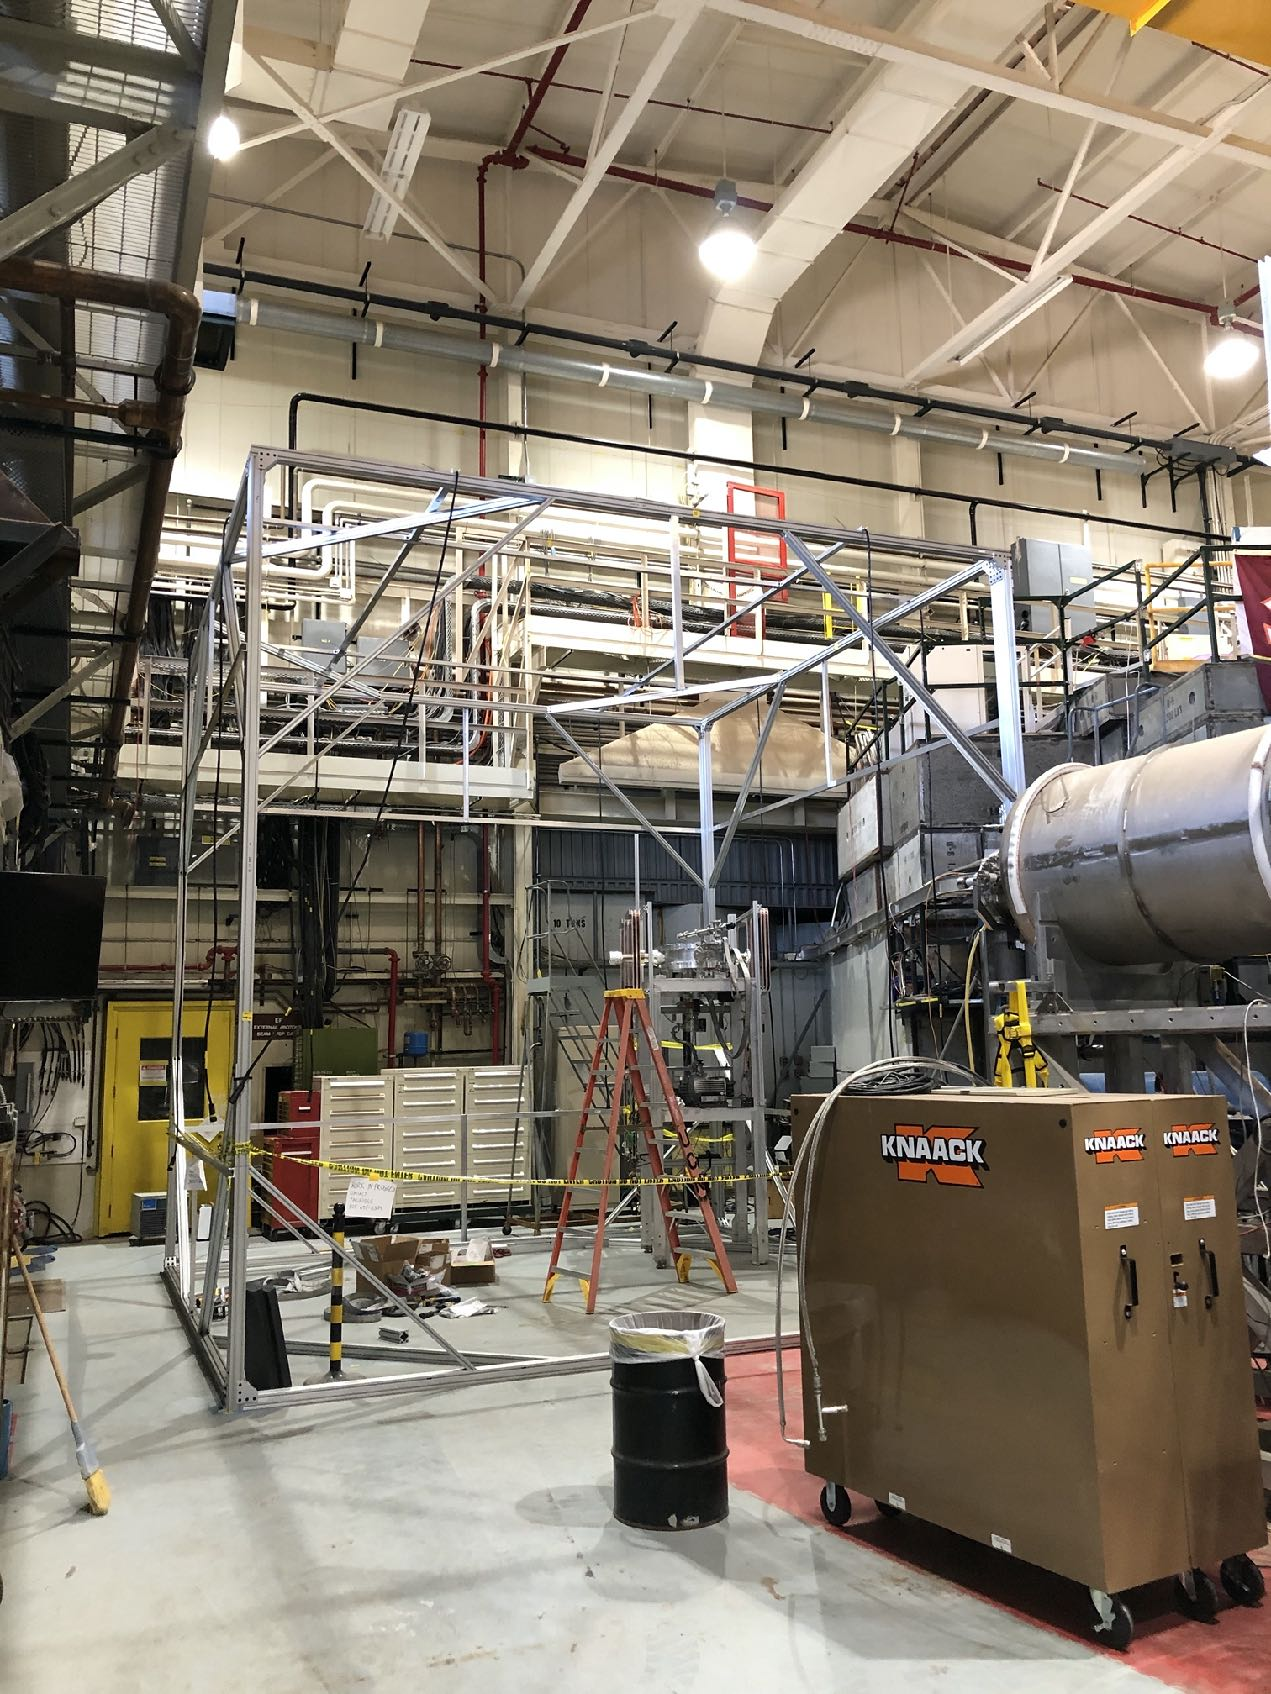
\includegraphics[height=4in]{figures/field_cage_no_msr.jpg}
    \caption
    {LANL nEDM field cage (Sec.~\ref{sec:field-cage})}
    \label{fig:lanl-field-cage}
\end{minipage}%
\begin{minipage}{.5\textwidth}
    \centering
    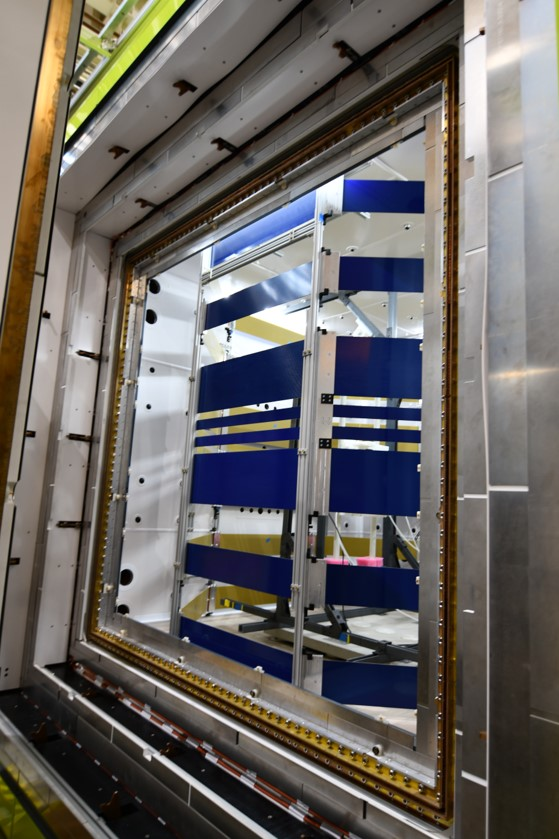
\includegraphics[height=4in]{figures/b0_zoom_in.jpg}
    \caption
    {Installed $B_0$ coil (Sec.~\ref{sec:B0_coil})}
    \label{fig:lanl-b0-coil}
\end{minipage}
\end{figure}

\begin{figure}
\centering
\begin{minipage}{.5\textwidth}
    \centering
    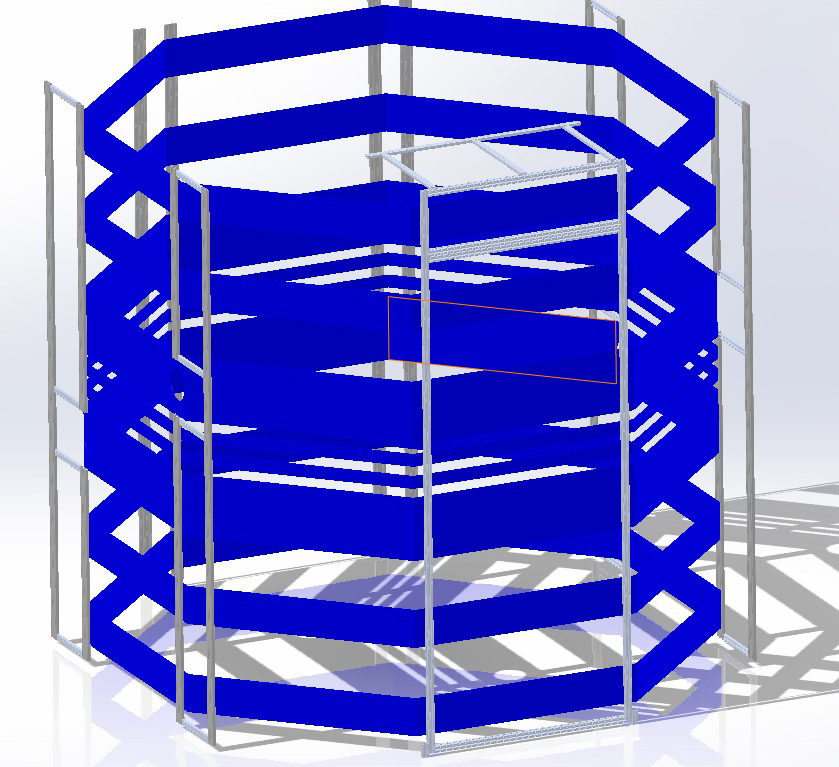
\includegraphics[width=0.9\textwidth]{figures/B0-model.png}
    \caption
    {Model of $B_0$ coil}
    \label{fig:b0-coil-model}
\end{minipage}%
\begin{minipage}{.5\textwidth}
    \centering
    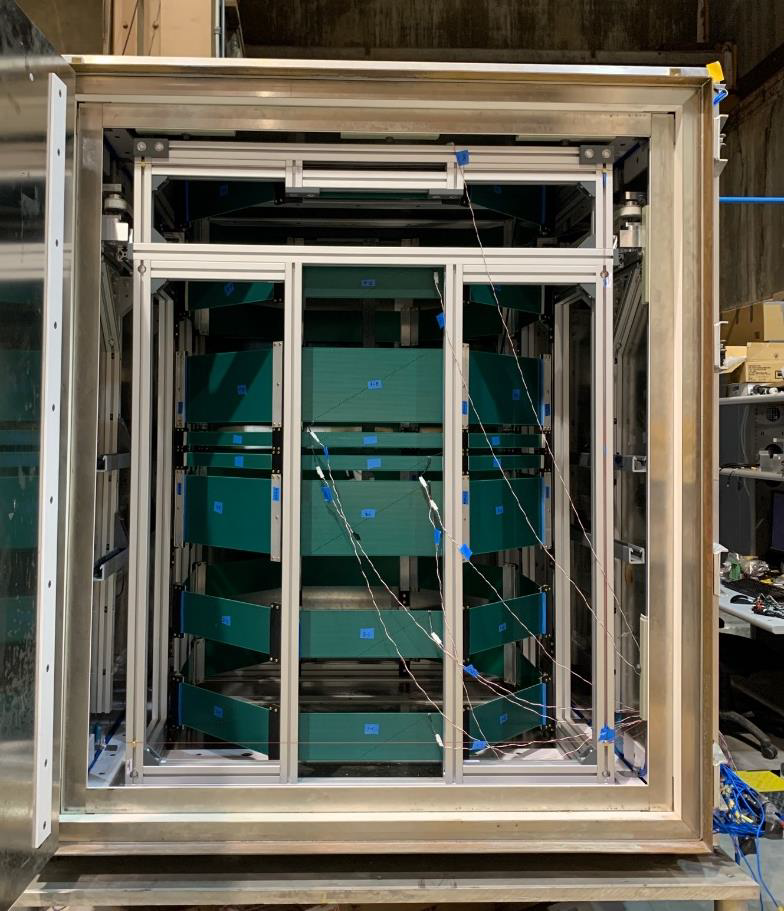
\includegraphics[width=0.9\textwidth]{figures/half-scale-B0.png}
    \caption
    {Half-scale $B_0$ coil prototype in the 2-layer MSR}
    \label{fig:b0-half-scale}
\end{minipage}
\end{figure}

The external compensation coils, or ``field cage,'' (Fig.~\ref{fig:lanl-field-cage}) provide up to \qty{32}{\micro\tesla} to offset ambient fields. The coil dimensions of the field cage are $\qty{5.3}{m}\times\qty{5.3}{m}\times\qty{5.3}{m}$. In the eventual LANL nEDM experiment a PID controller will enable active reduction of external field drifts.

%%%%%%%%%%%%%%%%%%%%%%%%%%%%%%%%%%%%%%%%%

\section{
    \texorpdfstring{$B_0$ coil}
                {B0 coil}\label{sec:B0_coil}
}

%%%%%%%%%%%%%%%%%%%%%%%%%%%%%%%%%%%%%%%%%

The LANL nEDM $B_0$ holding coil is a split solenoid consisting of 8 octagonal sections (Figs.~\ref{fig:lanl-b0-coil}, \ref{fig:b0-coil-model}). The design was inspired by the ``gapped solenoid'' described in Ref.~\cite{gosling_gapped_solenoid_1974}. Each section comprises of printed circuit boards (PCBs) and custom 3D-printed connections. The gaps between each section serve the purpose of accomodating neutron guides, comagnetometer lasers, \acrshort*{hv} cables, vacuum pump lines, etc. The modularized $B_0$ design allows removal of PCB segments from the octagon for access to the experiment. The $B_0$ coil is coupled to the innermost layer of the MSR for purposes of flux return. 

Field uniformity is adjusted by tuning the currents in each section of the coil. While initial measurements with fluxgates indicate that the vertical gradient meets specifications $(\partial B_0/\partial z < \qty{1}{nT \per m})$, further $B_0$ field uniformity measurements have been delayed due to the issue with the degaussing loop contacts (Sec.~\ref{sec:MSR}).

The $B_0$ coil has undergone several prototyping stages. An initial prototype was constructed for the Ramsey demonstration in 2017 (Chap.~\ref{chap:lanl_ramsey_demonstration}). A half scale prototype was also tested at LANL in a 2-layer MSR (Fig.~\ref{fig:b0-half-scale}), with measurements compared to COMSOL simulations.

%%%%%%%%%%%%%%%%%%%%%%%%%%%%%%%%%%%%%%%%%

\section{Transport coils}\label{sec:transport_coils}

%%%%%%%%%%%%%%%%%%%%%%%%%%%%%%%%%%%%%%%%%

\begin{figure}
\centering
\begin{minipage}{.5\textwidth}
    \centering
    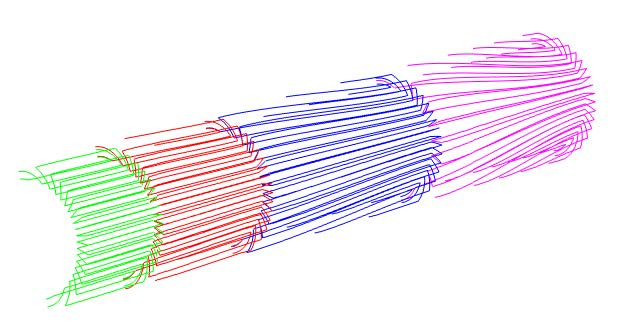
\includegraphics[width=\textwidth]{figures/transport_coil_mockup.jpg}
\end{minipage}%
\begin{minipage}{.5\textwidth}
    \centering
    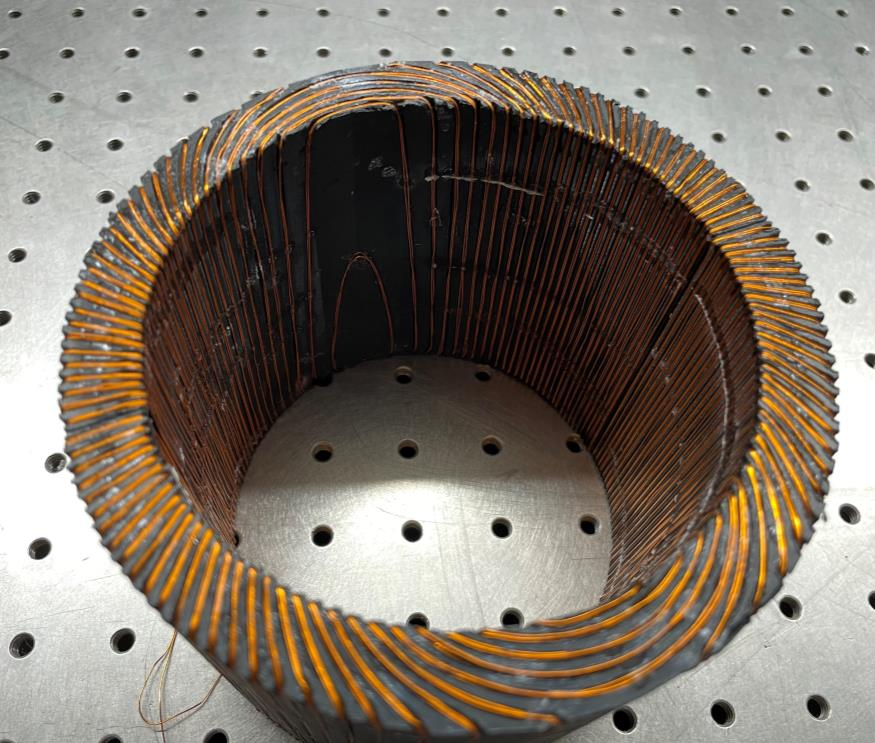
\includegraphics[width=\textwidth]{figures/transport_coil.jpg}
\end{minipage}
    \caption
    [Double layer $\cos\theta$ coil for transport from Earth's field to the $B_0$ field in the MSR.]
    {Double layer $\cos\theta$ coil for transport from Earth's field to the $B_0$ field in the MSR. Figure provided by Piya Amara Palamure.}
    \label{fig:transport-coils}
\end{figure}

A set of spin transport coils are used to adiabatically transport UCNs from the ambient external magnetic field ($\sim\qty{20}{\micro T}$) through multiple layers of MSR shielding to the $B_0$ holding field ($\sim\qty{1}{\micro T}$). The design is a modified double layer $\cos\theta$ coil, which generates a field along $z$ and provides self-shielding to limit the magnetization of surrounding $\mu$-Metal. Each of the MSR \ucn guide feed-throughs contain 4 segments of transport coils, which incrementally decrease in field magnitude. The innermost transport coil segments interface directly with $B_0$ PCB panels with a hole to avoid possible field zeros that would depolarize \ucn. 

%%%%%%%%%%%%%%%%%%%%%%%%%%%%%%%%%%%%%%%%%

\section{Magnetic Impurity Scanner}\label{sec:magnetic_impurity_scanner}

%%%%%%%%%%%%%%%%%%%%%%%%%%%%%%%%%%%%%%%%%

\begin{figure}
    \centering
    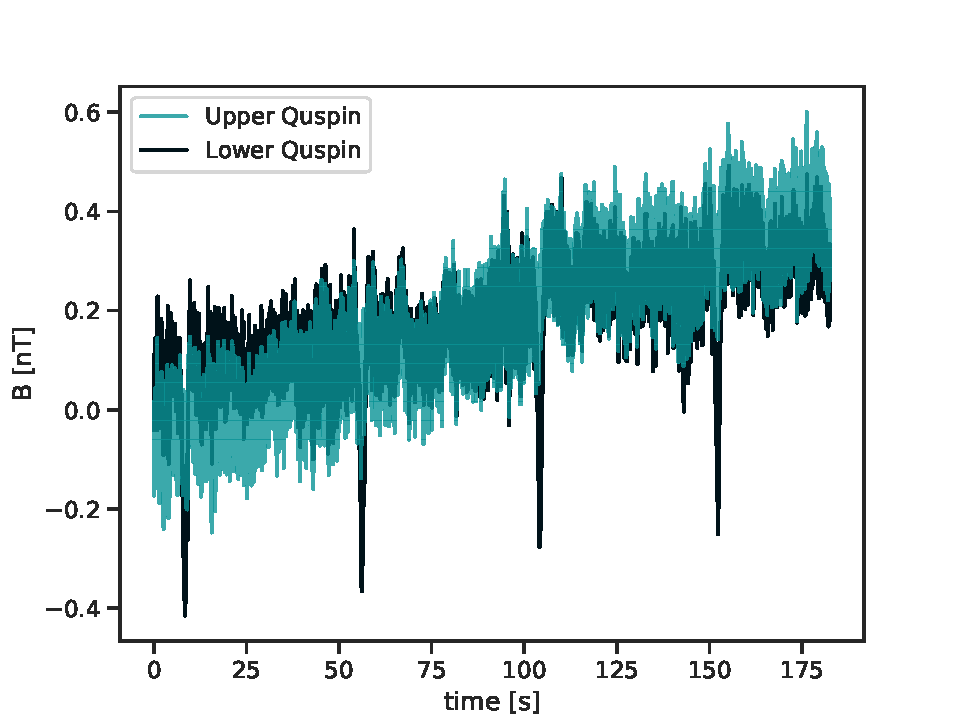
\includegraphics[width=0.7\textwidth]{figures/magnetic_contamination_example.pdf}
    \caption
    [Example of magnetic impurities on a rejected part found by the scanning setup in Sec.~\ref{sec:magnetic_impurity_scanner}. In this case, the aluminum  component contained threaded holes tapped with contaminated tooling.]
      {Example of magnetic impurities on a rejected part found by the scanning setup in Sec.~\ref{sec:magnetic_impurity_scanner}. In this case, the aluminum  component contained threaded holes tapped with contaminated tooling. The component is mounted on a slowly-moving turntable, and the periodic spike in the figure is correlated to when the part passes beneath the magnetometers. The QuSpin magnetometers are in a gradiometer configuration, such that there is a vertical separation between sensors of \qty{0.75}{in}.}
    \label{fig:magnetic_contamination_example}
\end{figure}

\begin{figure}
    \centering
    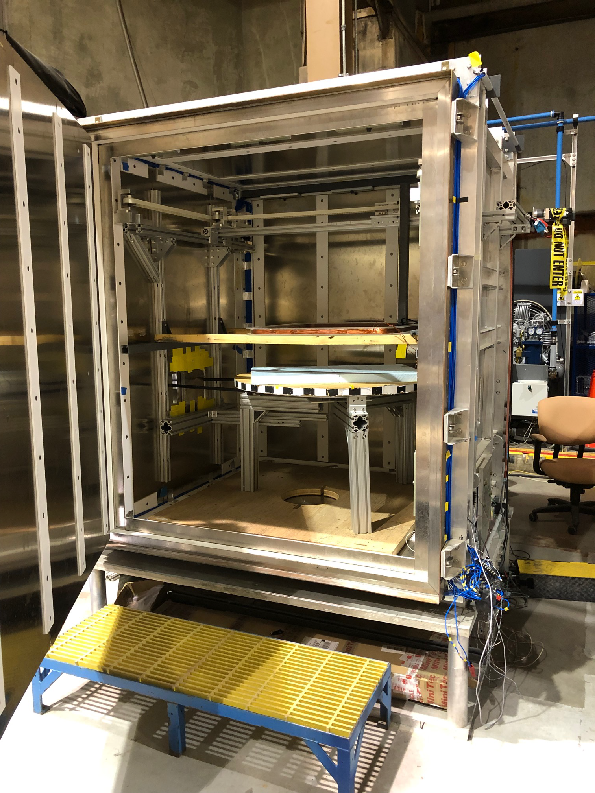
\includegraphics[height=3.5in]{figures/magnetic_impurity_scanner.png}
    \caption
      {Magnetic impurity scanner at LANL. In a 2-layer MSR, a nonmagnetic turntable passes parts beneath two QuSpin Total-Field Magnetometers.}
    \label{fig:magnetic_impurity_scanner}
\end{figure}

Localized magnetic sources (``contamination'') embedded within the precession cell and other experimental components create volume-averaged gradients that would lead to a false EDM signal. Any component installed within the MSR was subject to a scanning procedure to screen for contamination. Parts were mounted on a nonmagnetic turntable located in a 2-layer MSR at LANL (Fig~\ref{fig:magnetic_impurity_scanner}). The 2-layer MSR reduces the ambient magnetic field magnitude to $\leq \qty{50}{nT}$. The turntable was actuated by a belt system connecting to a motor outside the MSR. Parts were slowly passed beneath two Rb SERF magnetometers in a gradiometer configuration, where the vertical separation between sensors was \qty{0.75}{in}. Components with nonzero magnetic signal underwent additional cleaning, and, failing the re-screening procedure, were rejected from use within the MSR.

The current magnetic impurity scanner can detect contamination on the order of $\sim\qty{0.1}{nT}$. The magnetometers are QuSpin Total-Field Magnetometers, which have a sensitivity of $<\qty{1}{pT\per\sqrt{Hz}}$ in the 0.1--\qty{100}{\hertz} range. Use of these magnetometers required a small bias field provided by a large coil installed above the turntable. With improvements to the quality of the magnetic environment (e.g. extra shielding, reduced ambient magnetic noise) it will be possible to switch to QuSpin Zero-Field Magnetometers, which have a sensitivity $<\qty{1}{pT\per\sqrt{Hz}}$ for 1--\qty{100}{\hertz}.

Appendix~\ref{appx:magnetic_contamination} demonstrates the characterization process for a source of magnetic contamination found on a rejected component.

%%%%%%%%%%%%%%%%%%%%%%%%%%%%%%%%%%%%%%%%%

\section{Polarizing magnet}\label{sec:PM_description}

%%%%%%%%%%%%%%%%%%%%%%%%%%%%%%%%%%%%%%%%%

A \qty{5}{\tesla}, horizontal warm bore, superconducting magnet by American Magnetics Inc. is used as a polarizing magnet (\acrshort*{pm}). The PM field filters UCN spins, acting as a potential barrier that rejects low-field seeking UCN below \qty{300}{\nano\eV} and a potential well that passes high-field seeking UCN (Sec.~\ref{sec:ucn_polarizers}). 

A \qty{0.1}{\milli\meter} thick Al97 Mg3 alloy foil (similar in tensile strength to 6061-T6), termed the ``PM window," is located in the beamline at the center of the PM field region. This is used to separate the UCN source vacuum from the measurement apparatus vacuum, as the source vacuum can be routinely filled with D$_2$ gas (e.g. while D$_2$ is being drawn from a storage tank to be frozen or while SD$_2$ is being reconditioned). The magnetic potential of the PM overwhelms the neutron optical potential of the window (\qty{54}{\nano\eV} \cite{golubUCN}). The effect of the window on the transmission of UCN is discussed in detail in Sec.~\ref{sec:analysis}.

%%%%%%%%%%%%%%%%%%%%%%%%%%%%%%%%%%%%%%%%%

\section{UCN detectors}\label{sec:ucn_detectors}

%%%%%%%%%%%%%%%%%%%%%%%%%%%%%%%%%%%%%%%%%

We use $\ce{^{10}B}$-coated ZnS:Ag scintillator films for UCN detection \cite{jeph_b10_2011}. UCN are captured on the top layer of $\ce{^{10}B}$, and reaction products ($^4$He and/or $^7$Li) from the $\ce{^{10}B}(\text{n},\alpha)^7\text{Li}$ neutron capture reaction are detected in the ZnS:Ag layer. The resulting scintillation light is then transmitted through a light guide to a photomultiplier tube (\acrshort*{pmt}) or silicon photomultiplier (\acrshort*{sipm}).

%%%%%%%%%%%%%%%%%%%%%%%%%%%%%%%%%%%%%%%%%

\section{Spin flipper and analyzers}\label{sec:spin_flipper_analyzer}

%%%%%%%%%%%%%%%%%%%%%%%%%%%%%%%%%%%%%%%%%

Neutron spin analyzers in the LANL nEDM are 10 layer polarizers made of iron and silicon located immediately above neutron detectors (see Ref.~\cite{ThorstenThesis} for layer structure details). When magnetized with a ($\sim \qty{10}{mT}$) field from permanent magnets, the multi-layer polarizer preferentially transmits high-field seeking UCN and rejects low-field seeking UCN with an analyzing power of $99.3^{+0.7}_{-2.4}\%$~\cite{ThorstenThesis}.

Note that it is not clear if the neutron energy spectrum under which Ref.~\cite{ThorstenThesis} is consistent with the LANL nEDM neutron spectrum. Reference~\cite{afach_device_2015} quotes an analyzing power of 95\% for a different but similar analyzing foil for an energy range of 90~neV to 330~neV, which includes the energy range of the UCN at the analyzing foil for the experiment reported in Sec.~\ref{sec:analysis}. Additional analyzing power characterization measurements are planned.

An adiabatic fast passage (\acrshort{afp}) spin flipper coil, located upstream of the spin analyzer, is used to provide the option of spin flipping UCN (Sec.~\ref{sec:afp}).  Figure~\ref{fig:spin_flipper_efficiency} shows spin flipper performance (assuming perfect spin analyzing power) as a function of RF frequency. The minimum at \qty{20}{kHz}, \qty{10}{Vpp} is 0.12(1). The RF solenoid has a length of \qty{4}{in} and a diameter of $4\frac{7}{16}\text{ in}$. This corresponds to approximately 220 turns with 25 AWG wire. The inductance is \qty{4}{mH}. The solenoid is driven by a SRS DS345 function generator. 

The \qty{39}{in} vertical \ucn guide located above the spin analyzer is comprised of NiMo-coated glass, to avoid attenuation of the spin flipper amplitude. A schematic of the polarizing, spin analyzing, and detector system is illustrated in Fig.~\ref{fig:SpinAnalyzer}. The combined system is generally referred to as the ``drop detector.''

\begin{figure}
    \centering
    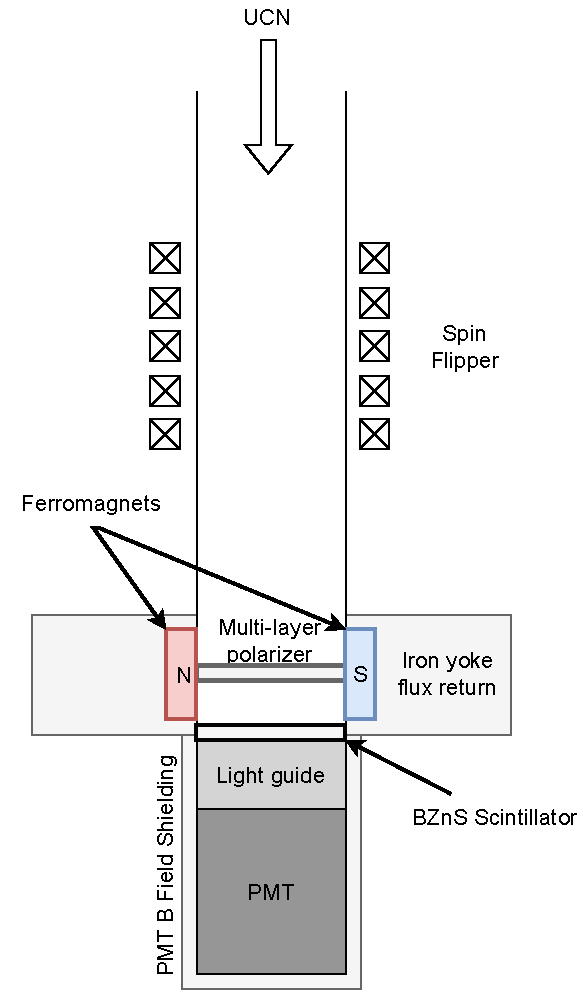
\includegraphics[width=5cm]{spinAnalyzer.pdf}
    \caption{Schematic of the ``drop detector,'' which consists of an adiabatic fast passage (\acrshort{afp}) spin flipper, polarizing foil, iron yoke flux return, light guide, and PMT}
    \label{fig:SpinAnalyzer}
\end{figure}

\begin{figure}
    \centering
    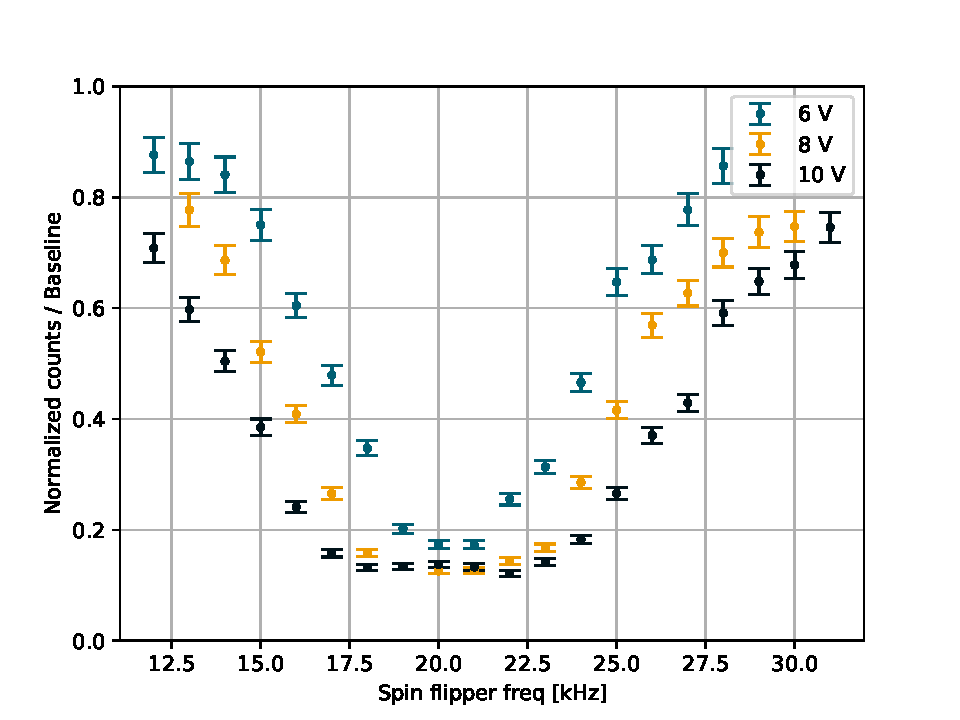
\includegraphics[height=3.5in]{figures/spin_flipper_efficiency.pdf}
    \caption
    [Measured UCN rate as a function of the RF spin flipper frequency and amplitude on the drop detector (Fig.~\ref{fig:SpinAnalyzer}).]
    {Measured UCN rate as a function of the RF spin flipper frequency and amplitude on the drop detector (Fig.~\ref{fig:SpinAnalyzer}). The $y$-axis is normalized using an upstream beamline monitor and then divided by the baseline UCN rate when the UCN spin flipper is off (c.f. Sec.~\ref{sec:ssa_measurements}). The minimum at \qty{20}{kHz}, \qty{10}{Vpp} is \qty{0.125(4)}.}
    \label{fig:spin_flipper_efficiency}
\end{figure}



%%%%%%%%%%%%%%%%%%%%%%%%%%%%%%%%%%%%%%%%%

\section{UCN switchers}\label{sec:lanl_switchers}

%%%%%%%%%%%%%%%%%%%%%%%%%%%%%%%%%%%%%%%%%

\begin{figure}
    \centering
    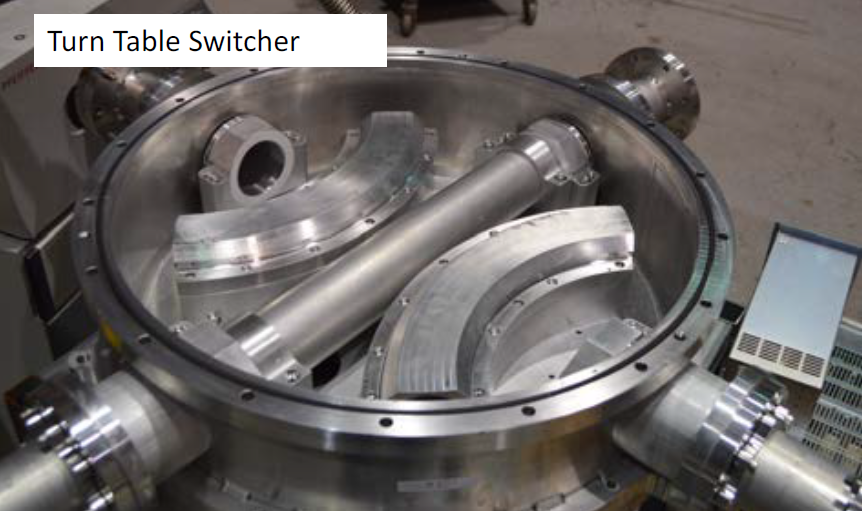
\includegraphics[width=7cm]{NewSwitcher.png}
    \hspace{1em}
    % 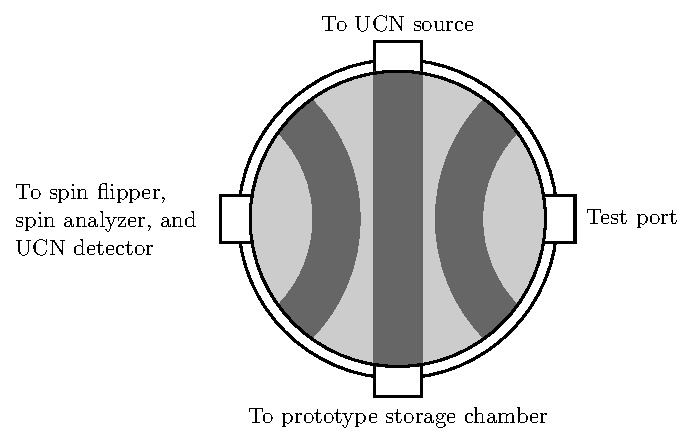
\includegraphics[width=0.5\textwidth]{North_Beamline_Switcher_Figure.pdf}
    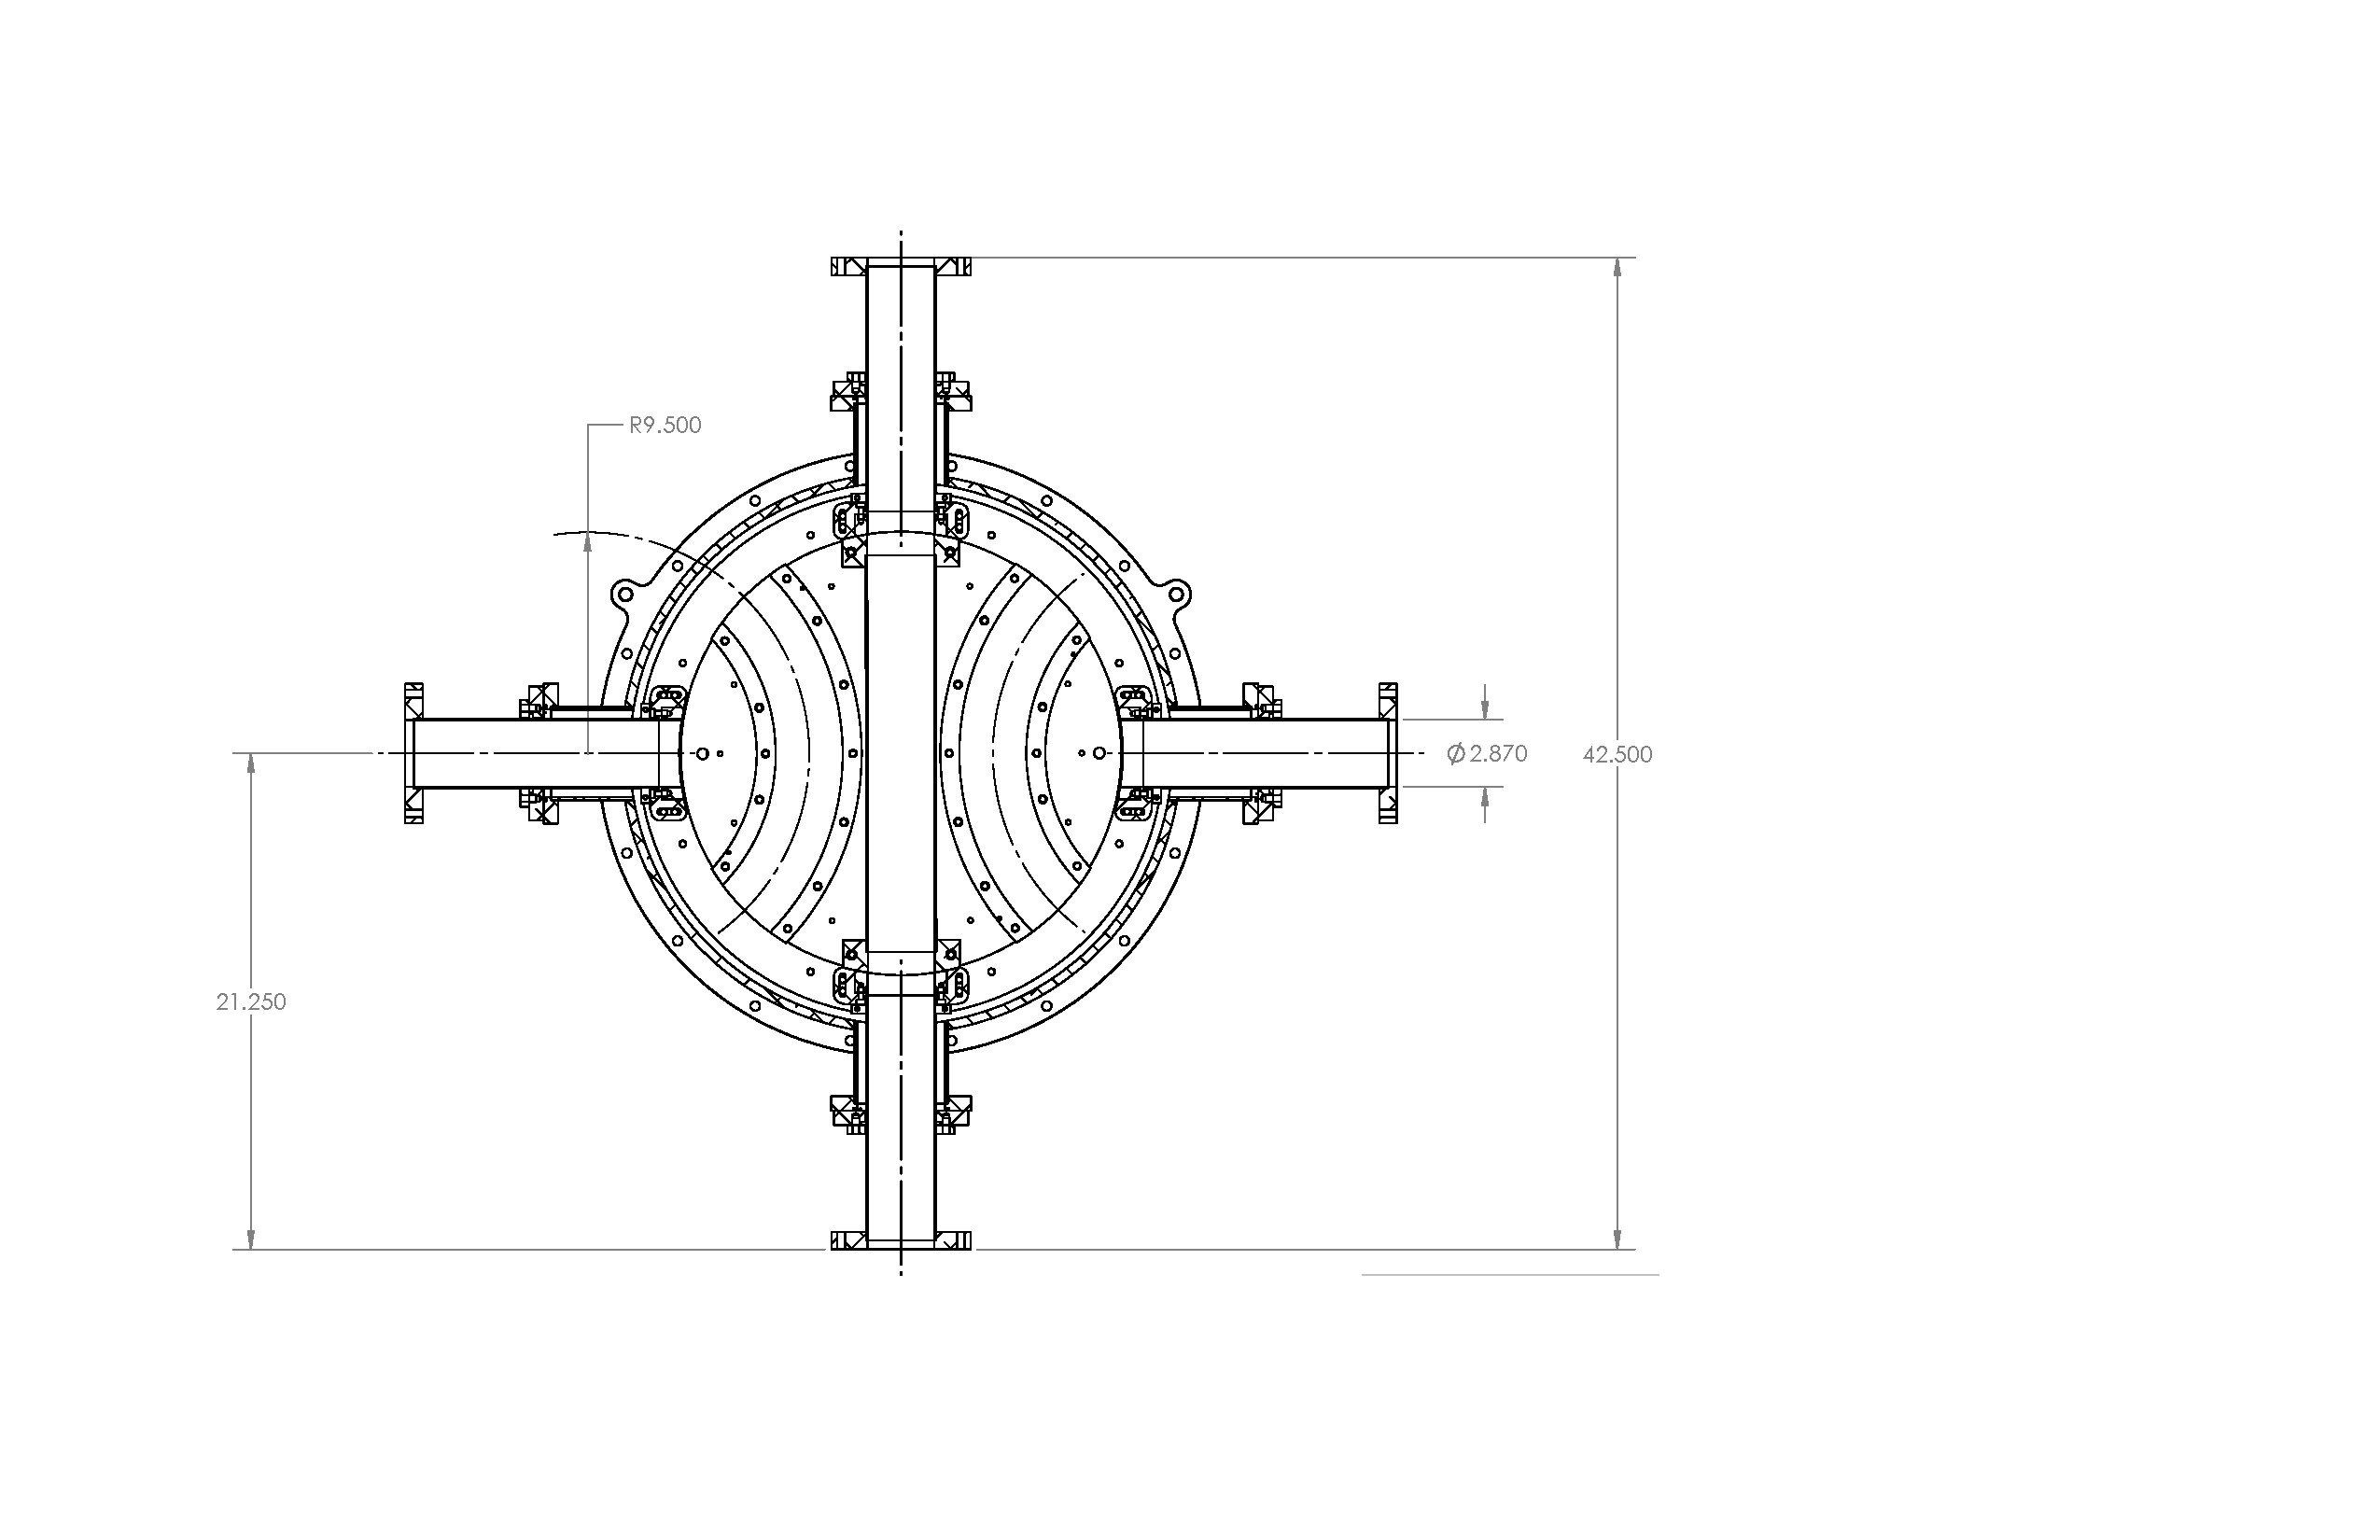
\includegraphics[width=0.5\textwidth]{figures/switcher_schematic.pdf}
    \caption[Photograph and schematic of rotary switcher]{Left: A photograph of the switcher, with the top removed. Right: Top-down schematic of the rotary switcher (courtesy of Chris O'Shaughnessy) }\label{fig:NewSwitcher}
\end{figure}

The LANL nEDM uses two switchers for neutron transport, one per precession cell. Each switcher has a cylindrical housing and four evenly spaced guide ports. These guide ports can be connected internally by either a straight guide section or \ang{90} bend sections. The internal guide sections are mounted on a rotating turntable and actuated by a Parker CM232DX servo-motor. Internal guide surfaces are coated with NiP and the interface of guide ports to the turntable-mounted guide sections is lined with PTFE to allow for minimal gaps between guide segments (see Tab.~\ref{tb:optical_potentials} for optical potentials). An image of the ``rotary switcher'' and a schematic of the guide segments within it are shown in Fig.~\ref{fig:NewSwitcher}. A study comparing the performance of this switcher design to a different prototype is performed in Chap.~\ref{chap:north_beamline_paper}.

%%%%%%%%%%%%%%%%%%%%%%%%%%%%%%%%%%%%%%%%%

\section{Precession cells}\label{sec:precession_cells}

%%%%%%%%%%%%%%%%%%%%%%%%%%%%%%%%%%%%%%%%%

\begin{figure}
    \centering
    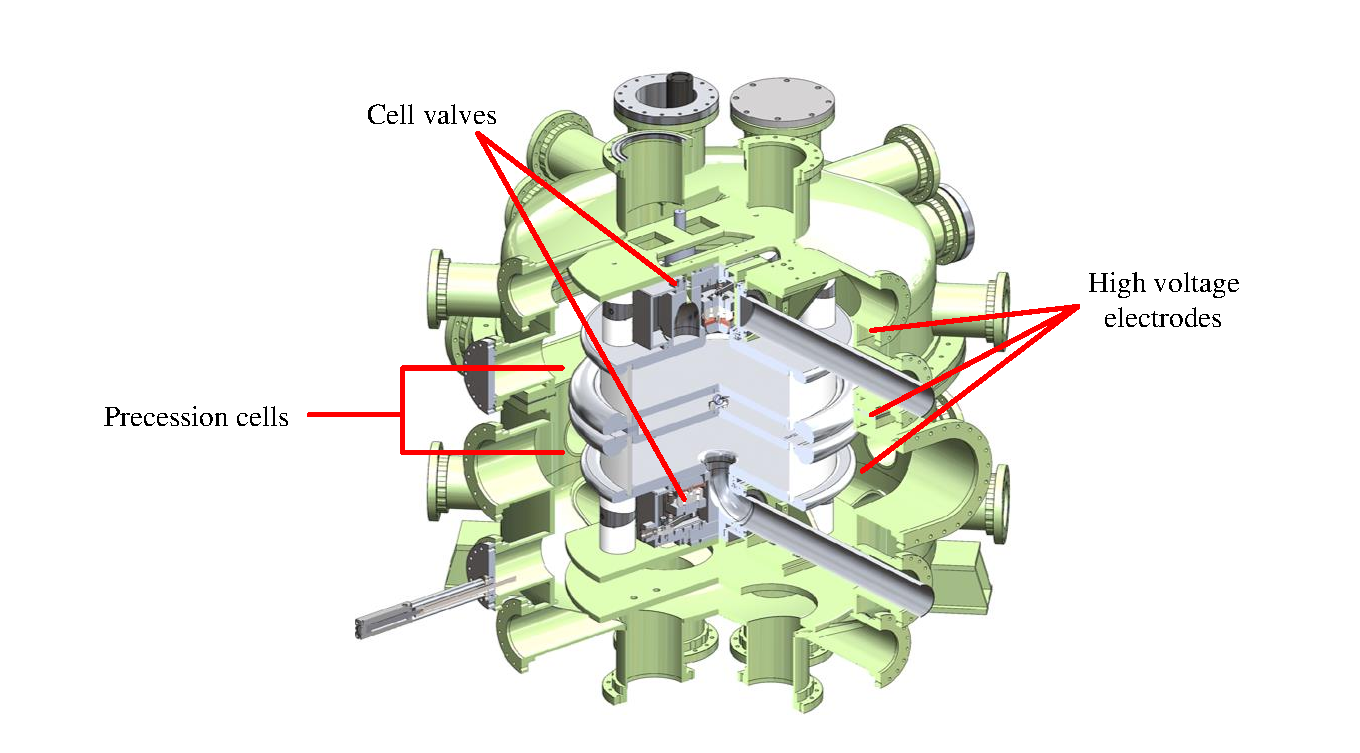
\includegraphics[width=0.85\textwidth]{figures/vacuum_chamber_cross.pdf}
    \caption
    {Cross section of the central apparatus, including the vacuum chamber, cell valves, HV electrodes, and precession cells}
    \label{fig:central_app_cross}
\end{figure}

\begin{figure}
\centering
\begin{minipage}{.5\textwidth}
    \centering
    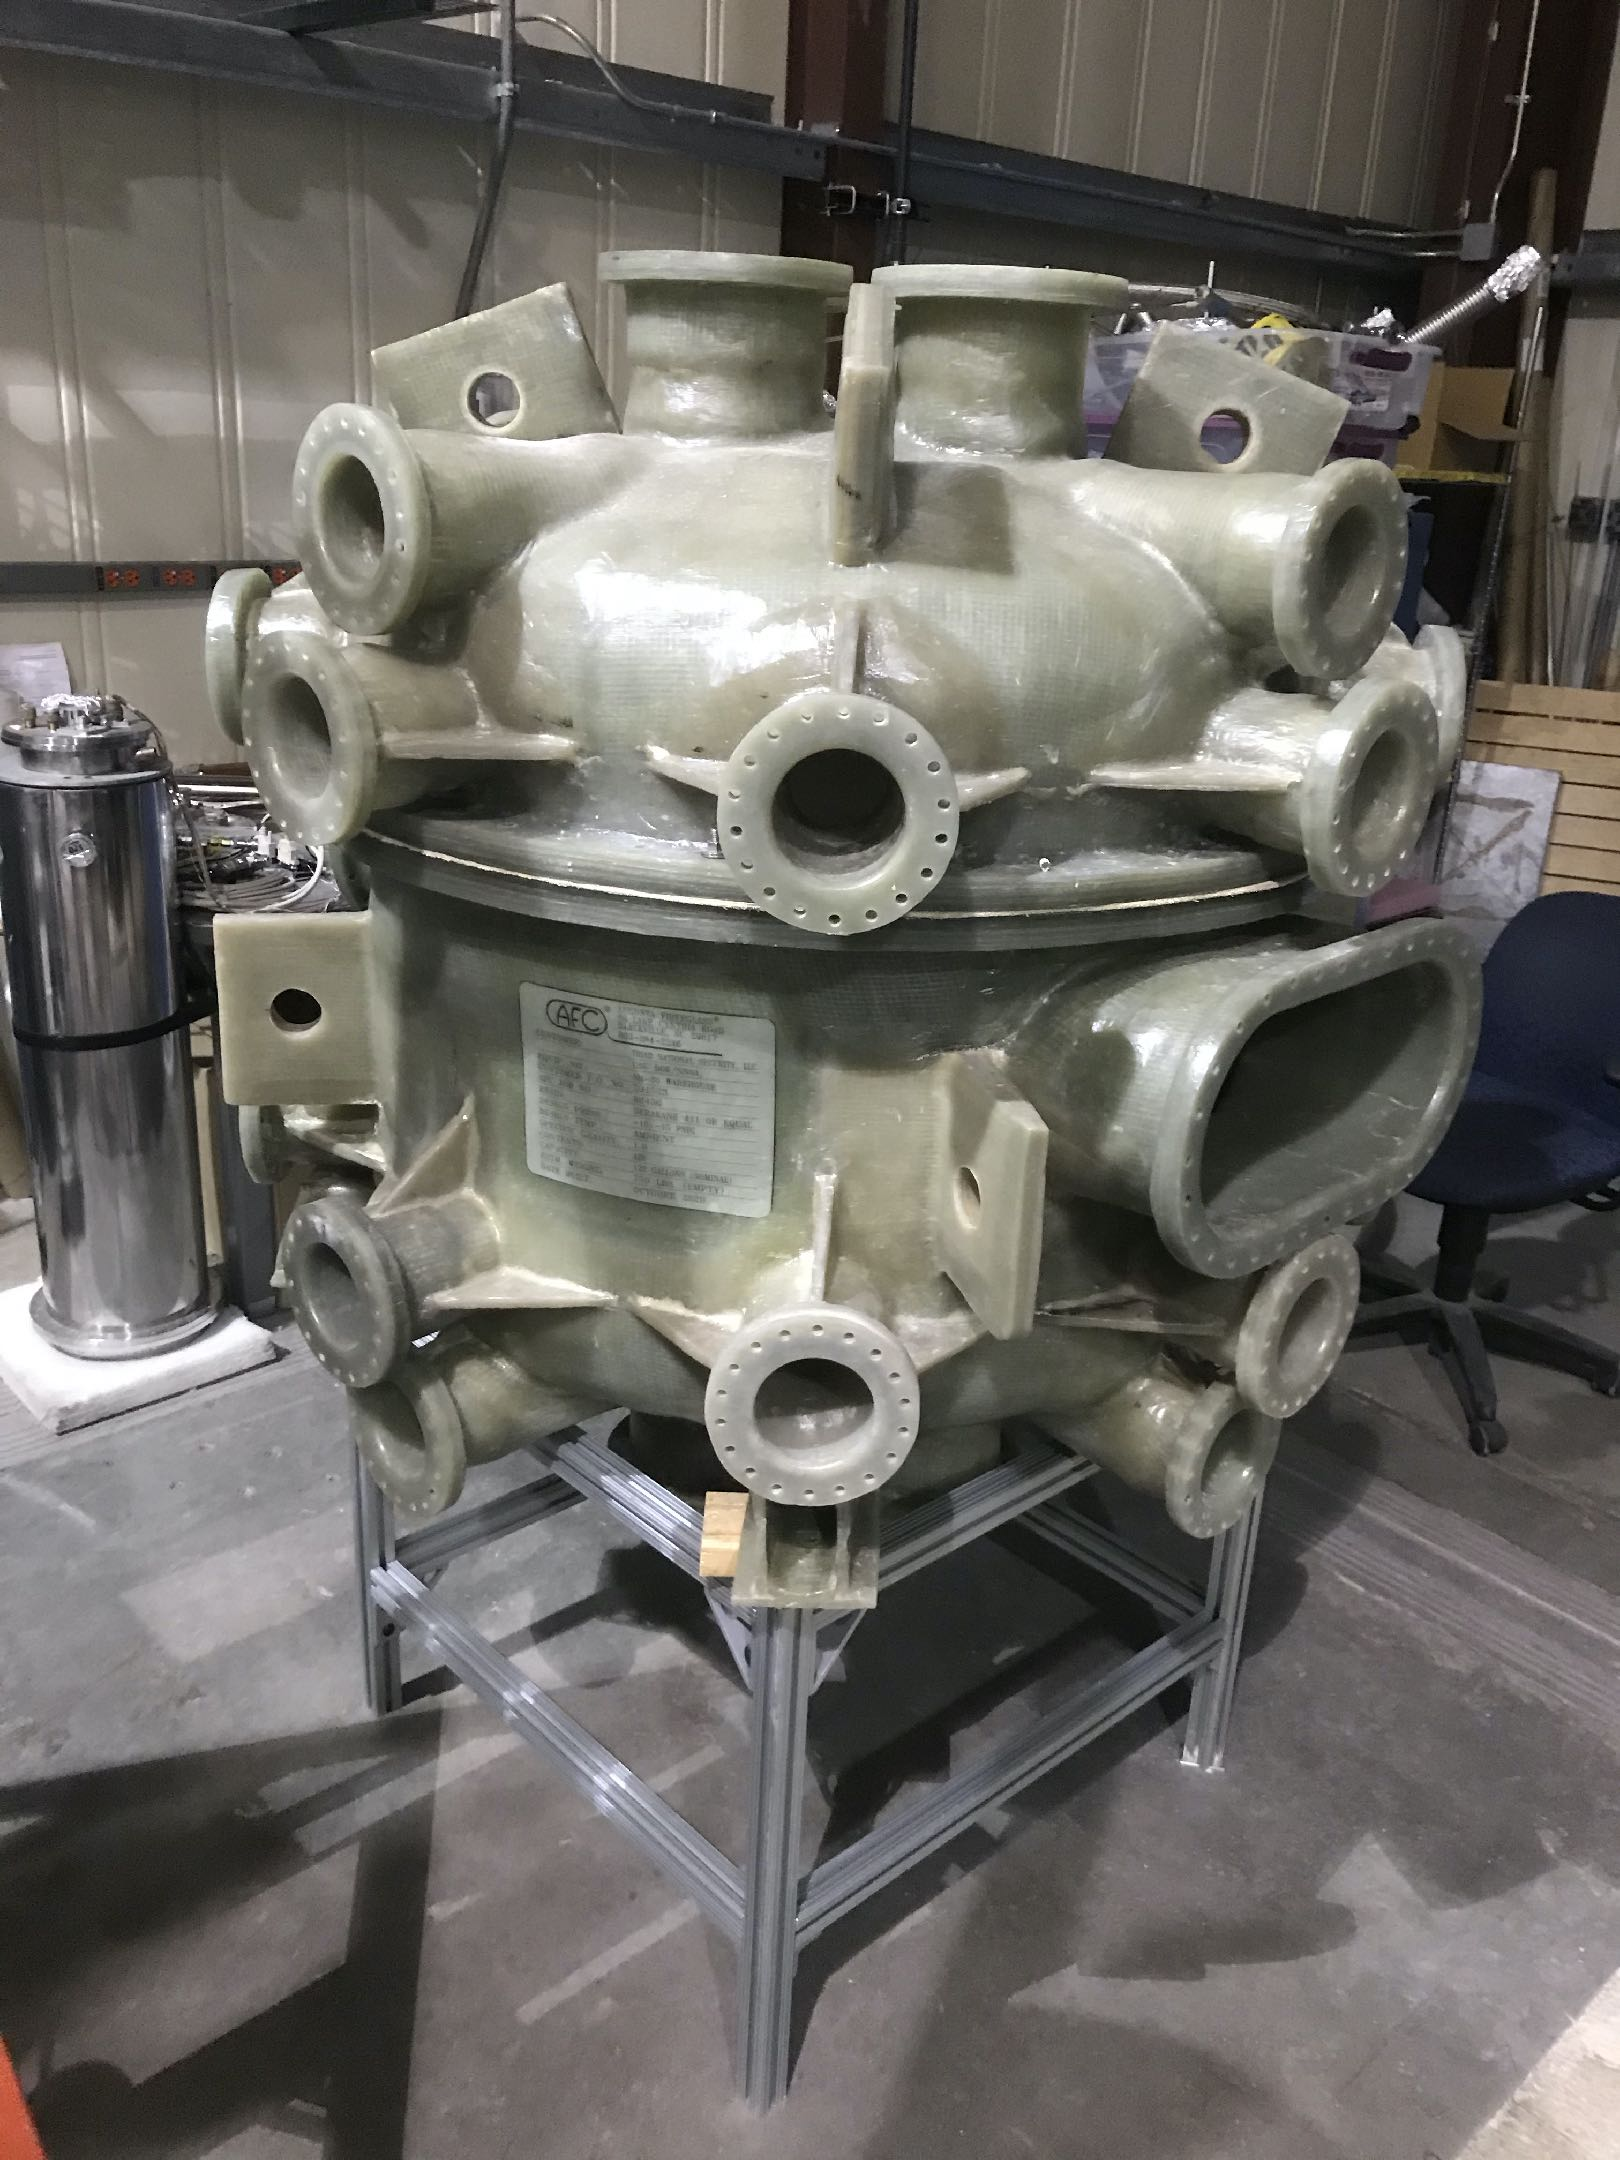
\includegraphics[height=4in]{figures/vacuum_chamber.jpg}
    \caption{Glass-epoxy vacuum chamber}
    \label{fig:vacuum_chamber}
\end{minipage}%
\begin{minipage}{.5\textwidth}
    \centering
    \includegraphics[width=4in,angle=90]{figures/cell_valve.jpg}
    \caption
    {Cell valve}
    \label{fig:cell_valve}
\end{minipage}
\end{figure}

The two precession cells, responsible for storage of polarized \ucn and \hg atoms, are each formed by parallel-plate electrodes sandwiching a poly(methyl methacrylate) (\acrshort*{pmma}) insulator. The PMMA cell walls are coated with deuterated polystyrene (\acrshort*{dps}) (Sec.~\ref{sec:dPS_coating}). The cells are designed with the ground electrodes on the top and bottom of the apparatus. The HV electrodes are concentrated in the middle, connected to a HV feedthrough. This enables simultaneous measurement of $\vv{B}_0\uparrow\uparrow\vv{E}$ and $\vv{B}_0\uparrow\downarrow\vv{E}$ configurations, cancellation of temporal field drifts to first order, and roughly doubles neutron counting statistics per cycle (see Sec.~\ref{sec:north_beamline_discussion}).

Each precession cell has an inner diameter \qty{50}{cm} and a height \qty{10}{cm}, a total volume of \qty{19.6}{\liter}. The final nEDM experiment will use electrodes coated in diamond-like carbon (\acrshort*{dlc}), though the measurements presented in this dissertation primarily use \acrshort{nip}-coated prototype electrodes (see discussion in Sec.~\ref{subsec:holdingTimeMeasurement}). 

The precession cells are enclosed by a custom glass-epoxy vacuum chamber from Augusta Fiberglass Coating Inc. (Fig.~\ref{fig:vacuum_chamber}). The material was selected to avoid attenuation of the RF $\pi/2$ pulse. Due to the vendor's lack of experience with high vacuum systems, work was required to make the chamber vacuum-tight, such as smoothing sealing surfaces with nonmagnetic sandpaper. 

The cell valves (Fig.~\ref{fig:cell_valve}) consist of Nickel Molybdenum (\acrshort*{nimo}) coated parts and NiP-coated guide segments mounted on G-10 fiberglass plates. The actuation system uses hydraulic lines filled with propylene glycol that are routed to a piston controlled by STM23Q motor outside of the MSR. This limits the production of undesired magnetic fields during cell valve actuation. Moving faces of the cell valve are sealed with PTFE-coated o-rings for maintenance of a separate vacuum from the vacuum chamber.

%%%%%%%%%%%%%%%%%%%%%%%%%%%%%%%%%%%%%%%%%

\subsection{Precession cell dPS coating}\label{sec:dPS_coating}

%%%%%%%%%%%%%%%%%%%%%%%%%%%%%%%%%%%%%%%%%

\begin{figure}
\centering
%subfigure width gets "multiplied" by includegraphics width
\begin{subfigure}{.5\textwidth} 
  \centering
  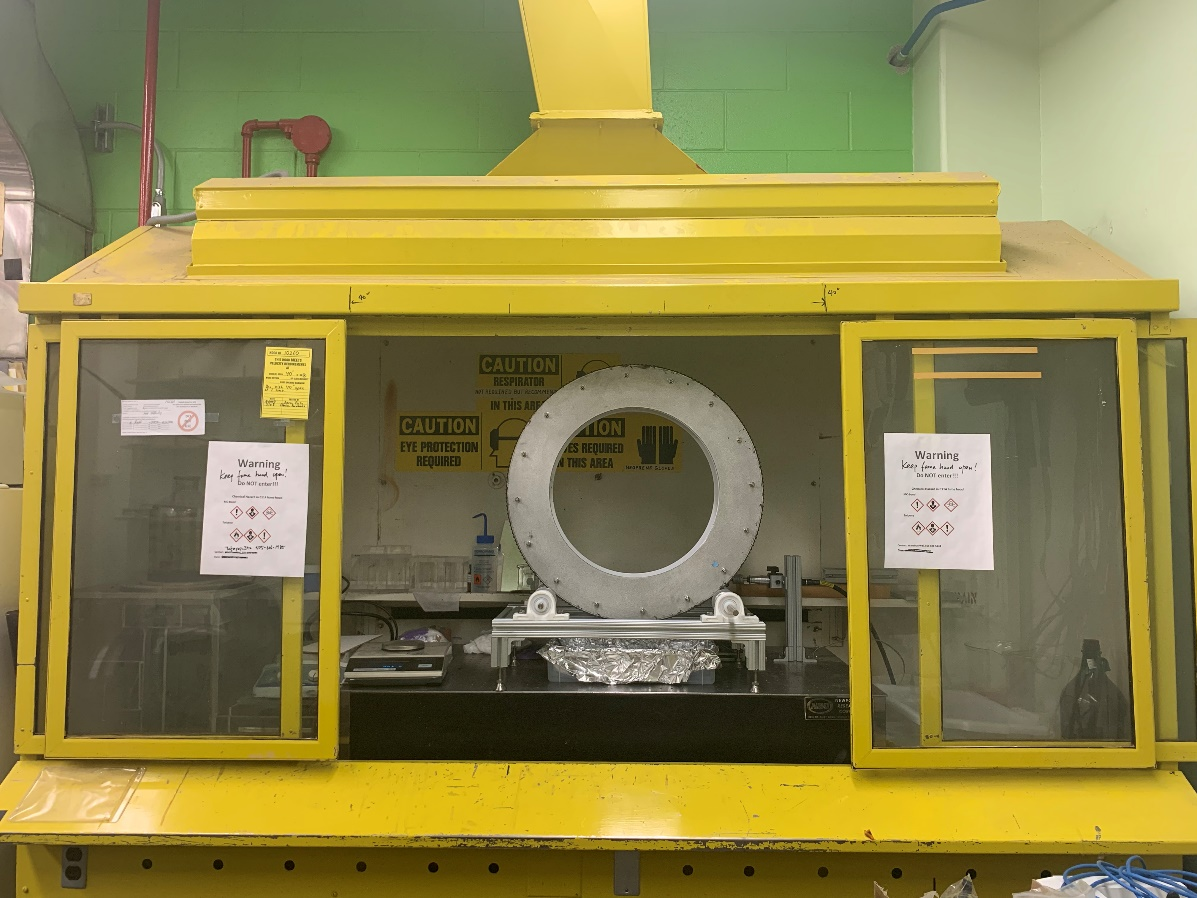
\includegraphics[width=\textwidth]{figures/dPS_jig_and_fume_hood.jpg}
\end{subfigure}%DO NOT REMOVE THIS '%'
\begin{subfigure}{.5\textwidth}
  \centering
  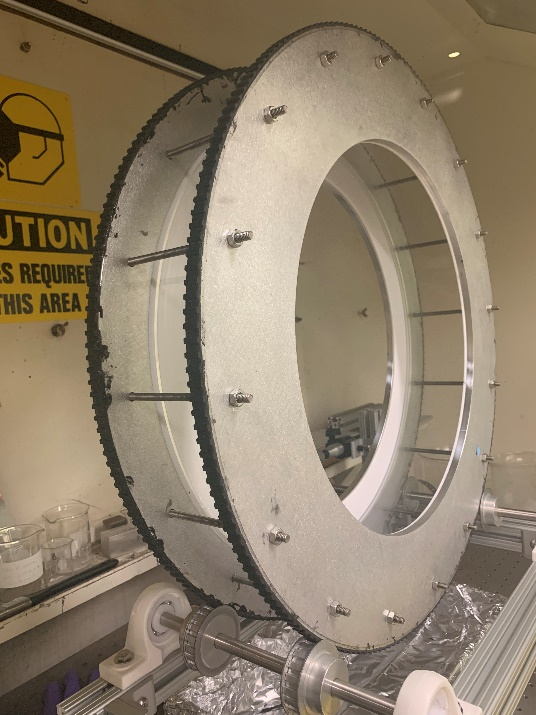
\includegraphics[width=0.57\textwidth]{figures/dPS_jig.jpg}
\end{subfigure}
\caption
{Precession cell wall dPS-coating jig, as described in Sec.~\ref{sec:dPS_coating}}
\label{fig:dPS_coating_jig}
\end{figure}

Two types of dPS coating methods were used for the PMMA precession cell walls. The first was a manual coating procedure, where the cell wall (oriented such that its central axis was horizontal) was slowly rotated over the course of an hour while a dPS/d-toulene mixture was applied with a brush (that was nonsolvent in toulene). This coating was tested in the prototype cell measurements in Chap.~\ref{chap:north_beamline_paper}.

The second coating method was the ``rotating lake'' described in Ref.~\cite{bodek_storage_2008}. The cell wall was clamped between two aluminum rings (Fig.~\ref{fig:dPS_coating_jig}), onto which the dPS/d-toulene mixture was poured. This was rotated slowly by a jig at roughly \qty{10}{rpm} for the entirety of the coating and drying process. This coating was used for measurements in Chap.~\ref{chap:nEDM_commissioning_dec2022}.

For both coating methodologies, \qty{1.5}{\gram} of dPS was dissolved into \qty{0.225}{\liter} d-toulene. The coated cell wall was allowed to dry in a fume hood for \qty{24}{\hour} and then outgassed under vacuum for a minimum of 2 weeks. When required, precession cells were vented with either dry nitrogen or argon to limit exposure of the cell wall to moisture.

%%%%%%%%%%%%%%%%%%%%%%%%%%%%%%%%%%%%%%%%%

\section{Cleaning procedure of UCN-friendly surfaces}

%%%%%%%%%%%%%%%%%%%%%%%%%%%%%%%%%%%%%%%%%

All NiMo, NiP, and Cu surfaces in the experiment that were exposed to UCN were subject to a gentle cleaning procedure to remove oils and dust. Surfaces were initially rinsed by a 1\% Alconox\textsuperscript{\textregistered} and deionized water solution. This was followed by a rinse in deionized water, which was then followed by a rinse from HPLC-grade isopropyl alcohol. Excess remaining isopropyl alcohol would be removed by a strong burst of dry nitrogen or argon. On the rare occassion that physical agitation was required to clean the surface, an AlphaWipe\textsuperscript{\textregistered} (or equivalent polyester wipe) with isopropyl alcohol was used. Special care taken to avoid scratching a coated surface or to leave any polyester fibers behind.
%%%%%%%%%%%%%%%%%%%%%%%%%%%%%%%%%%%%%%%%%%

\chapter{Ramsey method demonstration in prototype apparatus}\label{chap:lanl_ramsey_demonstration}

%%%%%%%%%%%%%%%%%%%%%%%%%%%%%%%%%%%%%%%%%%

This chapter summarizes a series of measurements taken on the North beamline in 2017 with an early prototype of the nEDM apparatus in a 2-layer \acrshort{msr} (Fig.~\ref{fig:ramsey_2017_apparatus}). Rabi and Ramsey fringes were produced, and measurements of spin relaxation lifetimes $T_1$ and $T_2$ were performed. 

%%%%%%%%%%%%%%%%%%%%%%%%%%%%%%%%%%%%%%%%%%%%%%

\section{Description of experimental setup (2017)}

%%%%%%%%%%%%%%%%%%%%%%%%%%%%%%%%%%%%%%%%%%%%%%


\begin{figure}[hb]
\centering
\begin{minipage}{.45\textwidth}
    \centering
    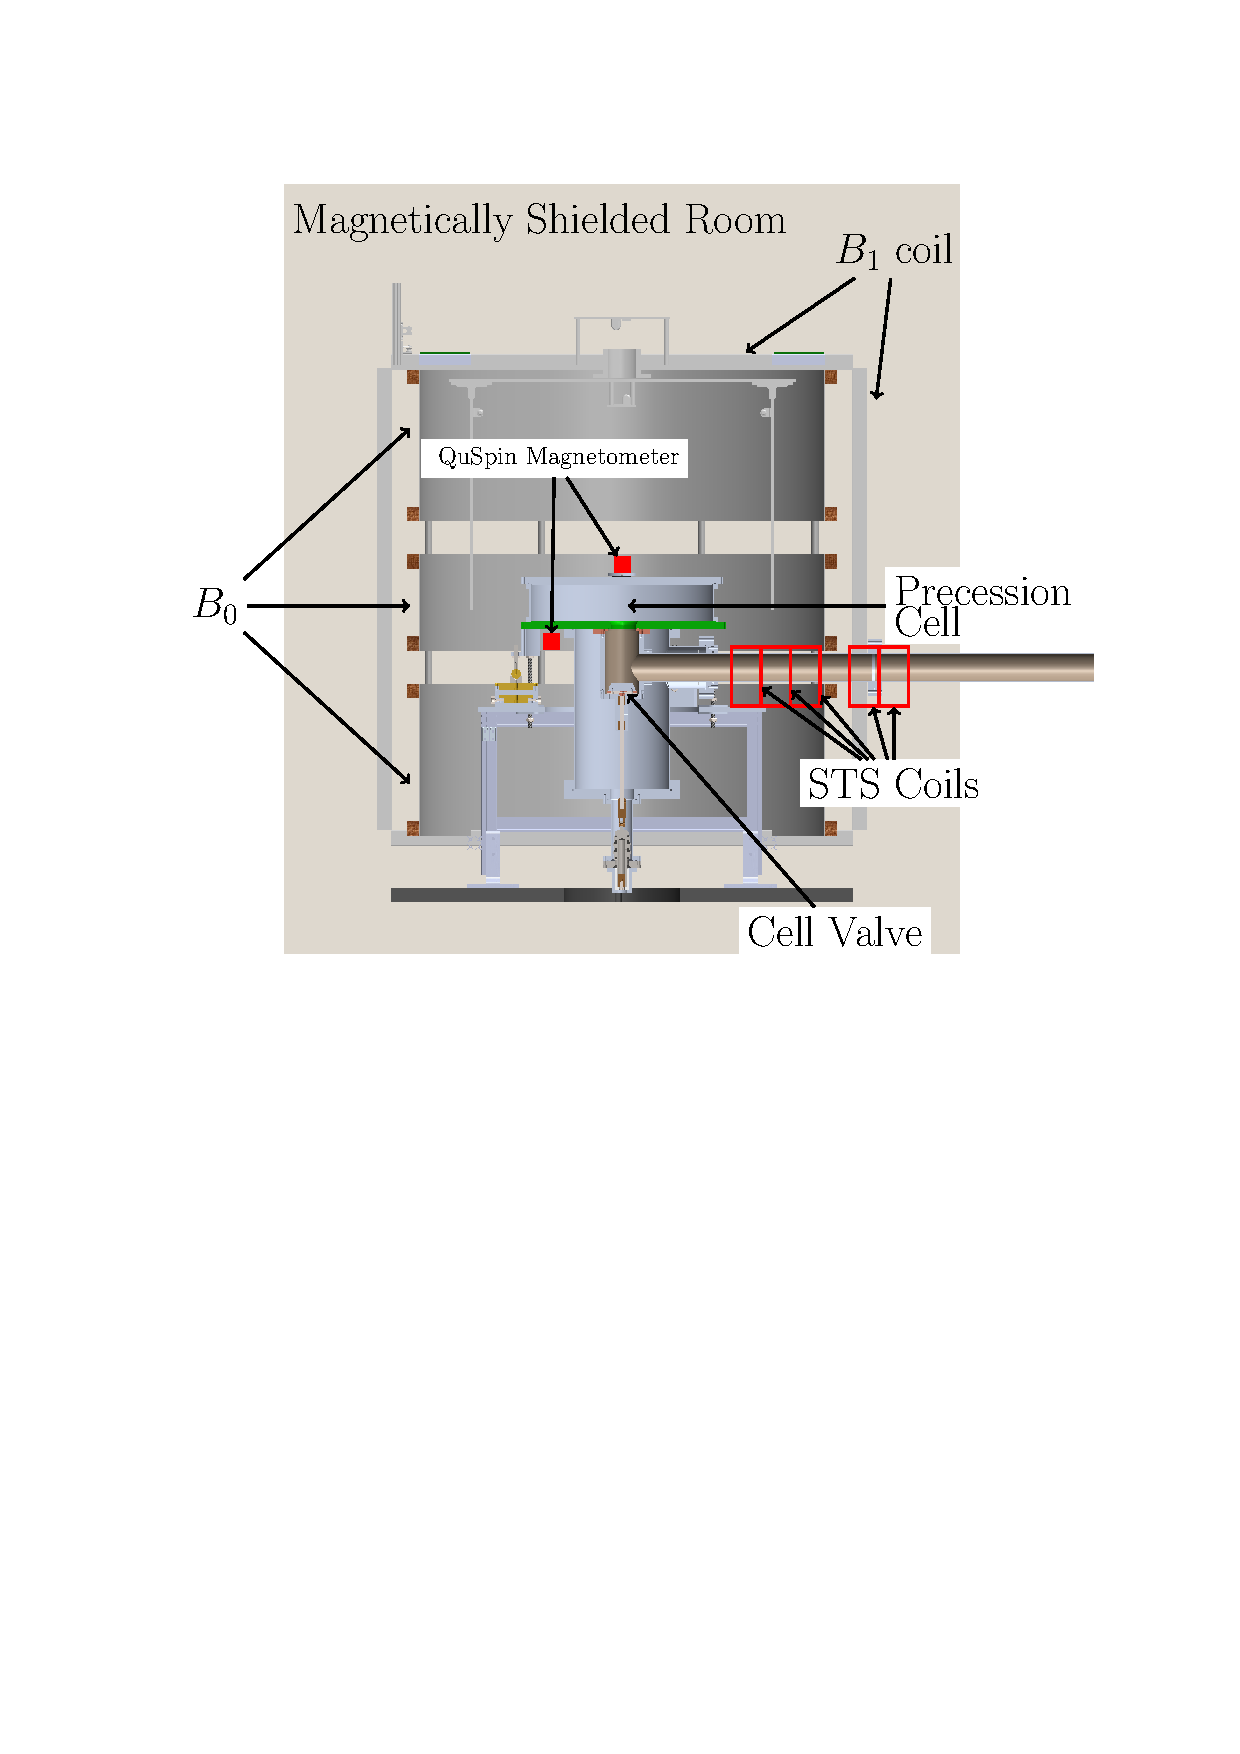
\includegraphics[width=\textwidth]{figures/ramsey2017_apparatus.pdf}
    \caption
    [Prototype experimental apparatus for measurements performed in 2017.]
    {Prototype experimental apparatus for measurements performed in 2017. Figure courtesy of Takeyasu Ito.}
    \label{fig:ramsey_2017_apparatus}
\end{minipage}%
\hspace{10pt}
\begin{minipage}{.45\textwidth}
    \centering
    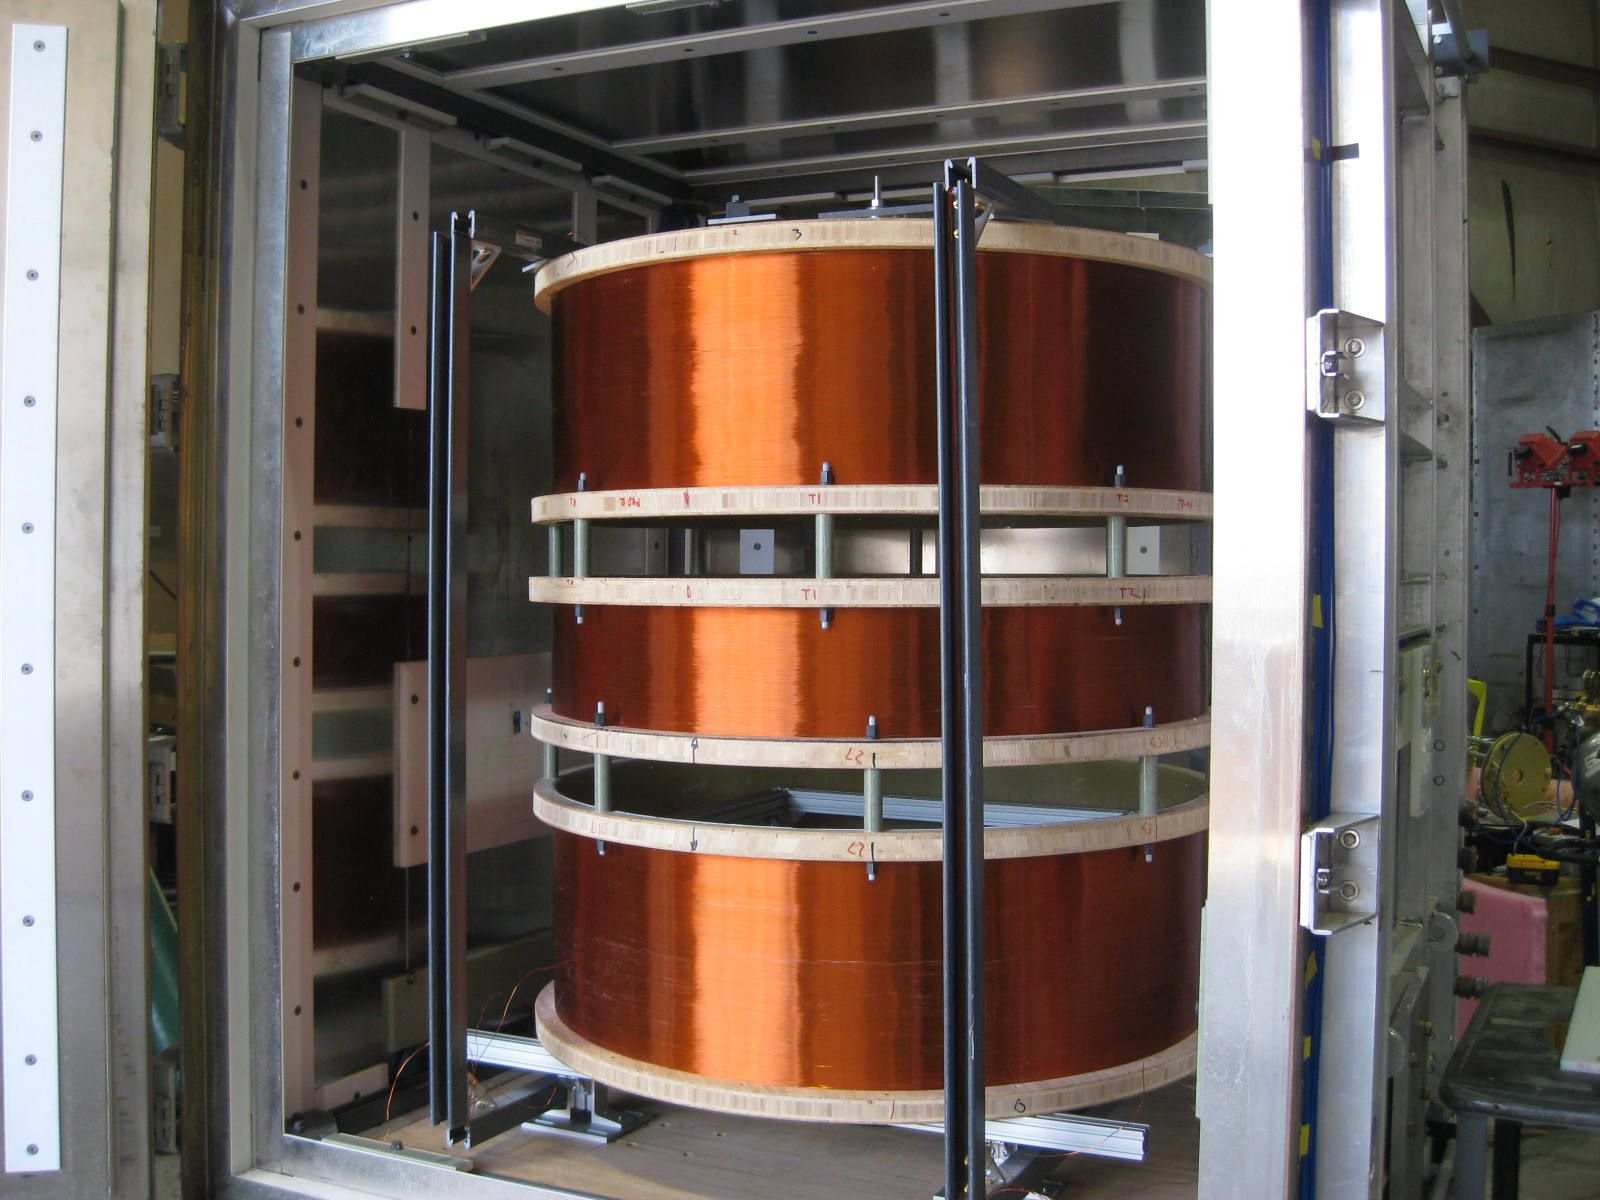
\includegraphics[width=0.9\textwidth]{figures/ramsey2017_B0_coil.jpg}
    \caption
    {$B_0$ coil prototype in the 2-layer MSR}
    \label{fig:ramsey_2017_B0_coil_prototype}
\end{minipage}
\end{figure}

Excepting the magnetic environment, the North beamline configuration in 2017 was largely equivalent to run condition 4 from Tab.~\ref{tb:runconditions} (layout depicted in Fig.~\ref{fig:NorthBeamlineLayout}), where the cell with dPS-walls, NiP electrode prototypes, rotary switcher, and drop detector used were the same as in Chap.~\ref{chap:north_beamline_paper}. For the 2017 measurement cycle, the window in the \acrshort{pm} region was comprised of \qty{50.8}{\micro\meter}-thick Al 5052 and the precession cell was housed in a 2-layer MSR. The 2-layer MSR reduced the ambient magnetic field to $\leq \qty{50}{nT}$. Two QuSpin Total Field magnetometers (sensitivity of $<\qty{1}{pT\per\sqrt{Hz}}$ in the 0.1--\qty{100}{\hertz} range) were used for field monitoring, one above the precession cell and one below. The magnetometers and MSR were later repurposed for the magnetic impurity scanner (Sec.~\ref{sec:magnetic_impurity_scanner}).

%%%%%%%%%%%%%%%%%%%%%%%%%%%%%%%%%%%%%%%%%%%%%%

\subsection
{
    \texorpdfstring{$B_0$ and transport coils}
                    {B0 and transport coils}
}

%%%%%%%%%%%%%%%%%%%%%%%%%%%%%%%%%%%%%%%%%%%%%%

\begin{figure}
    \centering
    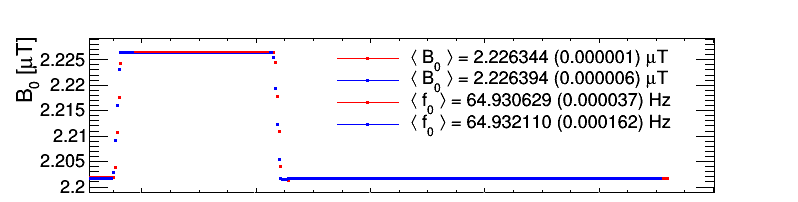
\includegraphics[width=0.8\textwidth]{figures/ramsey2017_B0.png}
    \caption
    [$|B_0|$ measured by the magnetometer located above the precession cell.]
    {$|B_0|$ measured by the magnetometer located above the precession cell. Blue and red lines refer to the measurement pair illustrated in Fig.~\ref{subfig:ramsey2017_t1_doublet}. The field drift between the two measurement periods was $\Delta B_0\approx\qty{50}{pT}$. When the STS transport coils were on during the fill and cell dump periods, $B_0\approx\qty{2.02}{\micro T}$.  During the measurement periods, $B_0\approx\qty{2.226}{\micro T}$. Figure courtesy of Robert Pattie Jr.}
    \label{fig:ramsey_2017_b0_map}
\end{figure}

An early prototype of the $B_0$ coil was constructed from 18 AWG copper wire wound about cylindrical fiberglass-reinforced plastic frames (Fig.~\ref{fig:ramsey_2017_B0_coil_prototype}). Opposite wound coils around the top and bottom of the $B_0$ prototype were used for shimming vertical magnetic field gradients to first order, such that the average value readouts from the QuSpins had overlapping error bars ($1\,\sigma$).

Because the $B_0$ prototype was not sufficiently coupled to the MSR for flux return, initial maps of the magnetic field profile with a fluxgate found a field zero along the \ucn beamline. Transport coils termed the segmented tapered solenoids (STS) were added to the interior of the MSR (Fig.~\ref{fig:ramsey_2017_apparatus}). The transport field oriented along the axis of the \ucn guide was incrementally reduced from $\sim\qty{50}{\micro T}$ to $\sim\qty{1}{\micro T}$ to facilitate spin transport in and out of the precession cell. Because the STS affected the quality of the $B_0$ field (Fig.~\ref{fig:ramsey_2017_b0_map}), the STS were only energized during filling and counting periods. With STS coils off and the cell valve closed, magnetometers read a value of $|B_0|=\qty{2.226}{\micro T}$.

As with the beamline configuration in Chap.~\ref{chap:north_beamline_paper}, guides between the MSR and the PM were kept under a $\sim\qty{1}{mT}$ magnetic field with coils for spin transport.

%%%%%%%%%%%%%%%%%%%%%%%%%%%%%%%%%%%%%%%%%%%%%%

\section
{
    \texorpdfstring{$T_1$ relaxation time measurement}
                    {T1 relaxation time measurement}
}\label{sec:2017_t1_measurement}

%%%%%%%%%%%%%%%%%%%%%%%%%%%%%%%%%%%%%%%%%%%%%%


\begin{figure}
\centering
%subfigure width gets "multiplied" by includegraphics width
\begin{subfigure}{.5\textwidth} 
  \centering
  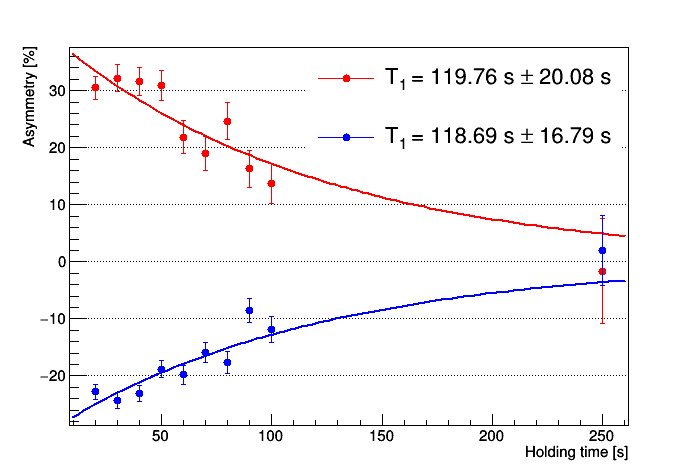
\includegraphics[width=\textwidth]{figures/ramsey2017_t1.png}
  \vspace{8pt}
  \caption{}\label{subfig:ramsey2017_t1_asymmetry}
\end{subfigure}%DO NOT REMOVE THIS '%'
\begin{subfigure}{.5\textwidth}
  \centering
  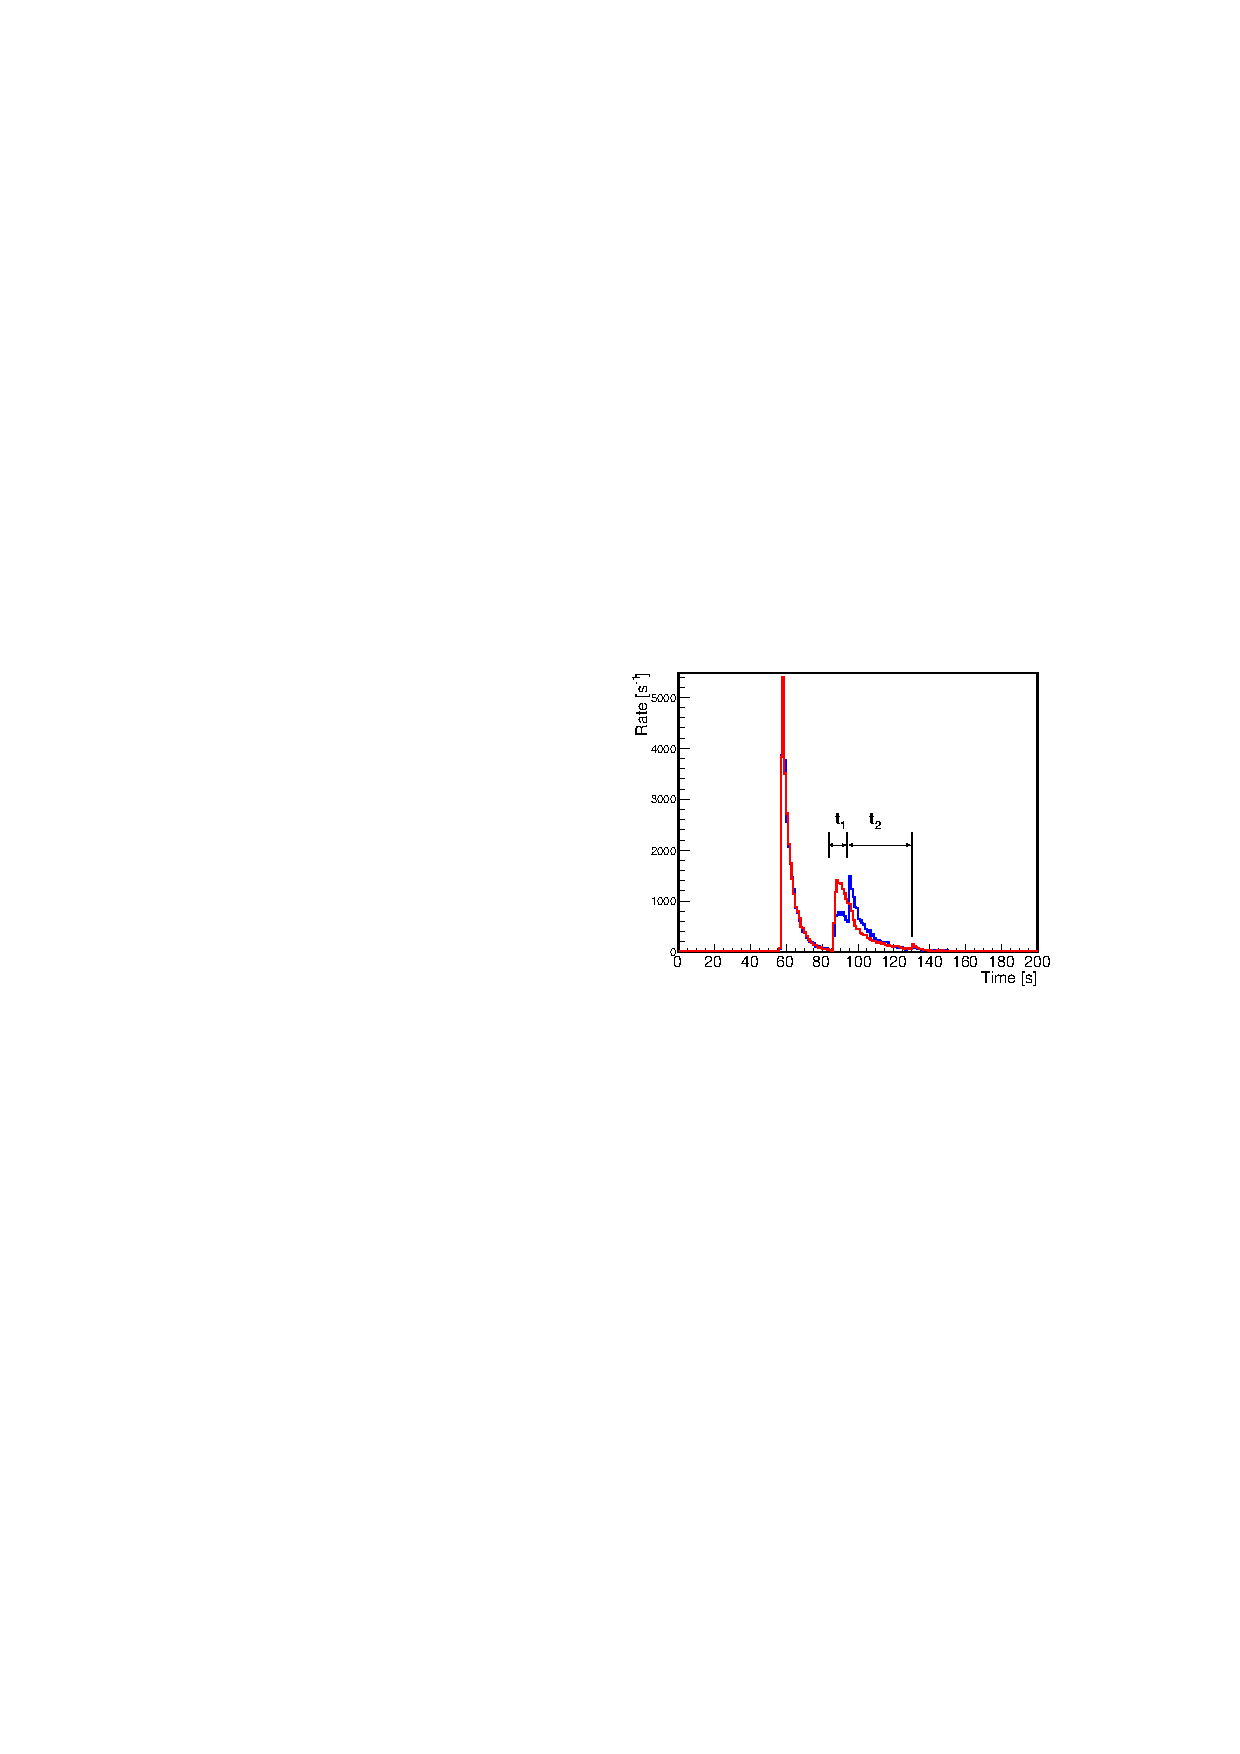
\includegraphics[width=\textwidth]{figures/ramsey_2017_t1_measurement_pair.pdf}
  \caption{}\label{subfig:ramsey2017_t1_doublet}
\end{subfigure}
\caption
    [Spin asymmetry as a function of holding time in the prototype apparatus.]
    {\textbf{(\subref{subfig:ramsey2017_t1_asymmetry})} Spin asymmetry as a function of holding time in the prototype apparatus. The red line refers to asymmetry during counting period $t_1$, and the blue line refers to asymmetry measured during counting period $t_2$. A fit of the measurements with a decaying exponential gives longitudinal spin relaxation time $T_1$. \textbf{(\subref{subfig:ramsey2017_t1_doublet})} Neutron count rate from a fill-and-dump run doublet. The red line refers to the sequence with the spin flipper toggling off-on-off during the cell dump, and blue refers to a on-off-on sequence. Figures by Robert Pattie Jr.}
\label{fig:ramsey_2017_t1}
\end{figure}

A measurement of longitudinal relaxation time $T_1$ (Sec.~\ref{sec:spin_relaxation}) was taken using the fill-and-dump sequence from Sec.~\ref{subsec:holdingTimeMeasurement} (Fig.~\ref{fig:timeSpectrum}). The preload period was \qty{45}{\second}, and the filling period was \qty{5}{\second}. Filling time was kept short to limit depolarization opportunity for \ucn in the guide system.

Storage times were varied from \qty{30}{\second} to \qty{250}{\second}. For each storage time parameter, two fill-and-dump runs (a ``run doublet'') with different counting sequences were performed. During the \qty{65}{\second} counting period, the spin flipper was off (on) for $t_1=\qty{10}{s}$, on (off) for $t_2=\qty{35}{s}$, and off (on) for \qty{20}{\second}. Figure~\ref{subfig:ramsey2017_t1_doublet} shows neutron count rate from a fill-and-dump run doublet with the labeled integration periods $t_1$ and $t_2$.

For an integration period $t_i$, the asymmetry $A_i$ is given by
%
\begin{gather}
    A_i=\frac{\Gamma_{\text{on, }i}-\Gamma_{\text{off, }i}}{\Gamma_{\text{on, }i}+\Gamma_{\text{off, }i}}
    \label{eq:spin_asymmetry} 
\end{gather}
%
where $\Gamma_i$ is the normalized number of UCN counted in the corresponding integration period, and the on/off subscript refers to the spin flipper state during $t_1$. Detector counts were normalized using the preload count rate on the West beamline monitor as per the procedure in Sec.~\ref{subsec:dataProcessing}. No cell valve leak was observed in the data from the 2017 measurement cycle. For holding times $<\qty{40}{s}$, the guide dump (Sec.~\ref{subsec:dataProcessing}) did not complete before the start of the counting period. In these cases, the guide dump was fit with a decaying exponential. The fit was then integrated over the counting period and was subtracted.

Assymetry (for both $t_1$ and $t_2$) as a function of storage time is shown in Fig.~\ref{subfig:ramsey2017_t1_asymmetry}. A fit of the measurements with a decaying exponential $A(t)=A_0\exp(-t/T_1)$ gives longitudinal spin relaxation time $T_1$. Fitting both curves Fig.~\ref{subfig:ramsey2017_t1_asymmetry} and calculating the average gave $\langle T_1 \rangle=\qty{199(13)}{s}$. 

In the limit $t=0$ (effectively 0 storage time), we have $A(0)\approx 0.3$. By comparison, a direct flow through mode measurement from the \ucn source to the drop detector (Fig.~\ref{fig:spin_flipper_efficiency}) gives $A(0)\approx 0.8$. In addition, changing the cell wall from dPS cell wall to NiP did not significantly change $T_1$, suggesting that the spin relaxation time was mostly the result of magnetic field gradients.

The gradient $\partial B_0 / \partial z$ in a precession cell can be estimated from $T_1$ using Eq.~(\ref{eq:T1_dBdZ_mcgregor}) (assuming no contribution to depolarization from wall bounces). We take the mean wall collision time $\tau_\text{c}=4V/(\overline{v}A)=\qty{36.7}{ms}$ (Appx.~\ref{appx:ucn_effusion}). This gives $\partial B_0/\partial z\approx \qty{12}{\micro G\per cm}$. At the time no in situ measurement method was available to confirm field gradient. It is likely that a stainless steel bellows in the prototype apparatus responsible for cell valve actuation was the source of the gradient. The bellows was replaced with a nonmagnetic version immediately after the 2017 measurement cycle.

%%%%%%%%%%%%%%%%%%%%%%%%%%%%%%%%%%%%%%%%%%%%%%

\section{Rabi measurement}\label{sec:2017_rabi_measurement}

%%%%%%%%%%%%%%%%%%%%%%%%%%%%%%%%%%%%%%%%%%%%%%

\begin{figure}
    \centering
    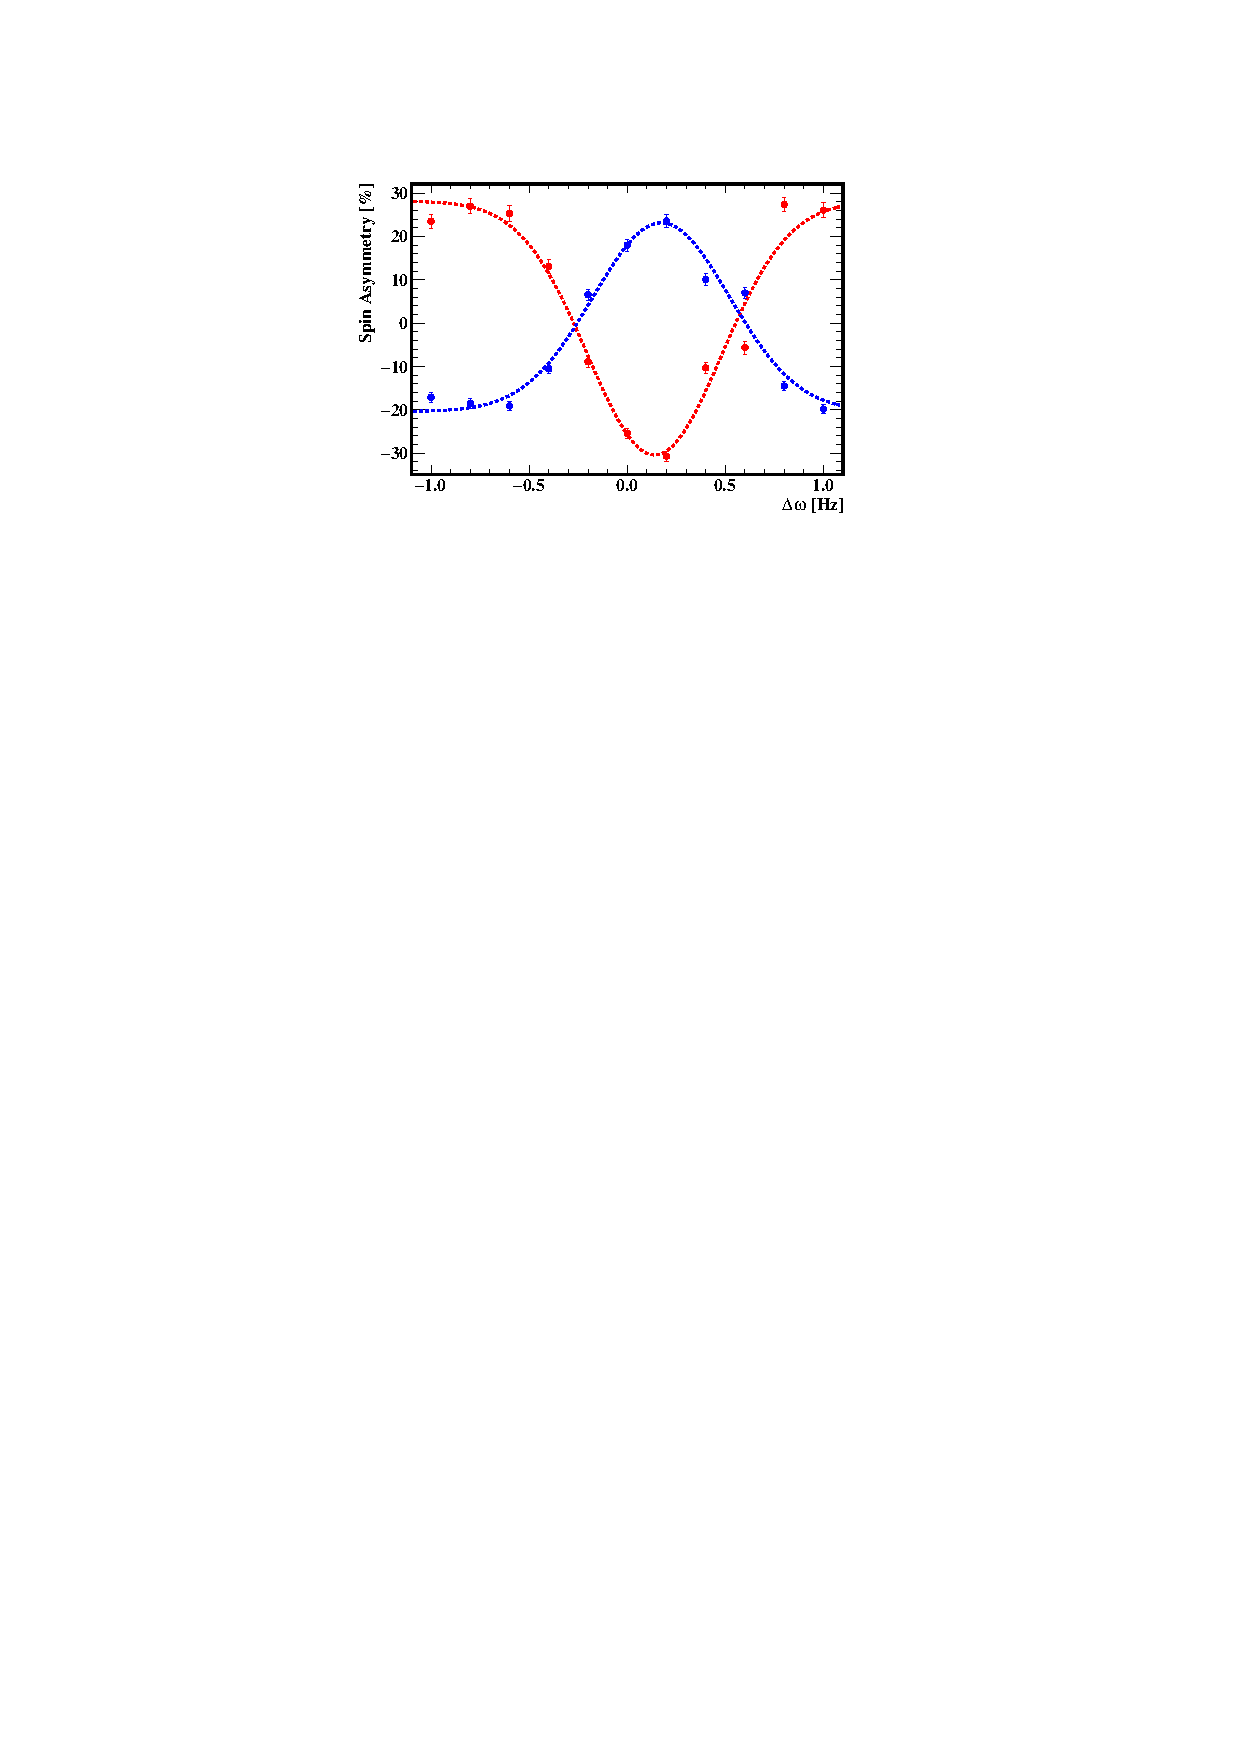
\includegraphics[width=0.55\textwidth]{figures/2017_rabi_fringe.pdf}
    \caption
    [Rabi fringe measured in the prototype apparatus.]
    {Rabi fringe measured in the prototype apparatus. A plot of spin asymmetry (\ref{eq:spin_asymmetry}) as a function of $\pi$ pulse frequency. Figure by Robert Pattie Jr.}
    \label{fig:rabi_fringe_2017}
\end{figure}

A Rabi fringe (Fig.~\ref{fig:rabi_fringe_2017}) was produced using the same run sequence as the $T_1$ measurements, with a \qty{30}{\second} storage time. \qty{5}{\second} after the start of the storage period, a \qty{1}{\second}-long $\pi$ pulse was applied. The frequency range of the Rabi fringe was $\qty{64.5}{Hz} \pm \qty{1}{Hz}$ with step size \qty{0.2}{Hz}. The spin asymmetry at each frequency step was calculated using Eq.~(\ref{eq:spin_asymmetry}). The fit of the Rabi fringe gave a resonant frequency of \qty{0.17(1)}{Hz}, with a full width half maximum of \qty{0.8(1)}{Hz}.

%%%%%%%%%%%%%%%%%%%%%%%%%%%%%%%%%%%%%%%%%%%%%%

\section{Ramsey measurement}\label{sec:2017_ramsey_measurement}

%%%%%%%%%%%%%%%%%%%%%%%%%%%%%%%%%%%%%%%%%%%%%%

Ramsey fringes (Fig.~\ref{fig:ramsey_fringes_2017}a--\ref{fig:ramsey_fringes_2017}c) were created with the same run parameters as the Rabi sequence, with two $\pi/2$ pulses each with duration \qty{0.5}{s} each. Three different precession times were used ($\gls*{T_fp}=\qty{1}{s},\,\qty{10}{s},\,\qty{20}{s}$). The total storage time was held constant at \qty{30}{\second}.

Spin asymmetry was calculated with the same procedure as Sec.~\ref{sec:2017_rabi_measurement}, and the maximal spin asymmetry for each Ramsey fringe was determined by fitting the fringe (see Eqs.~(\ref{eq:ramsey_fringe_modulation_N_cos}) and (\ref{eq:four_point_ramsey_fringe_fit})). A plot of max asymmetry as a function of free precession period is shown in Fig.~\ref{fig:ramsey_fringes_2017}d. We see that as \gls*{T_fp} has increased max asymmetry has decreased, which means that as \ucn are allowed to precess for longer periods of time the transverse spin gets increasingly relaxed. Therefore fitting a decaying exponential to the data in Fig.~\ref{fig:ramsey_fringes_2017}d is a measure of transverse relaxation time. This was found to be $T_2=19.5(2.7)\text{ s}$.

From Eq.~(\ref{eq:T2_mcgregor}) (again assuming negligible depolarization from wall bounces) we estimated the transverse gradient in the cell. We let diffusion constant $D_\text{ucn}\approx \qty{2.2}{m^2 \per s}$~\cite{golubUCN} from Eq.~(\ref{eq:ucn_diffusion_constant}), using the assumption that the chance of a diffuse reflection in the cell is of order $\sim 10\%$. Therefore, assuming transverse gradients along $x$ and $y$ are of roughly equally magnitude, we find $\partial B_z/\partial r \approx \qty{18}{\micro G \per cm}$. This is consistent with the estimate obtained in Sec.~\ref{sec:2017_t1_measurement}.

%%%%%%%%%%%%%%%%%%%%%%%%%%%%%%%%%%%%%%%%%%%%%%

\section{Pulse sequence instrumentation}

%%%%%%%%%%%%%%%%%%%%%%%%%%%%%%%%%%%%%%%%%%%%%%

The $\pi$ and $\pi/2$ pulses in Secs.~\ref{sec:2017_rabi_measurement}--\ref{sec:2017_ramsey_measurement} used a SRS DS345 with its amplitude modulated by a DG535 pulse generator. The precision of these devices in the context of the LANL nEDM experiment is discussed in Sec.~\ref{sec:pulse_gen_freq_std}. Appendix~\ref{appx:gpib_usb_pulse_sequence} provides the code used to set the pulse sequencing for the Rabi and Ramsey fringe measurements in this chapter.

\vspace{\baselineskip}

\begin{figure}[hbp]
    \centering
    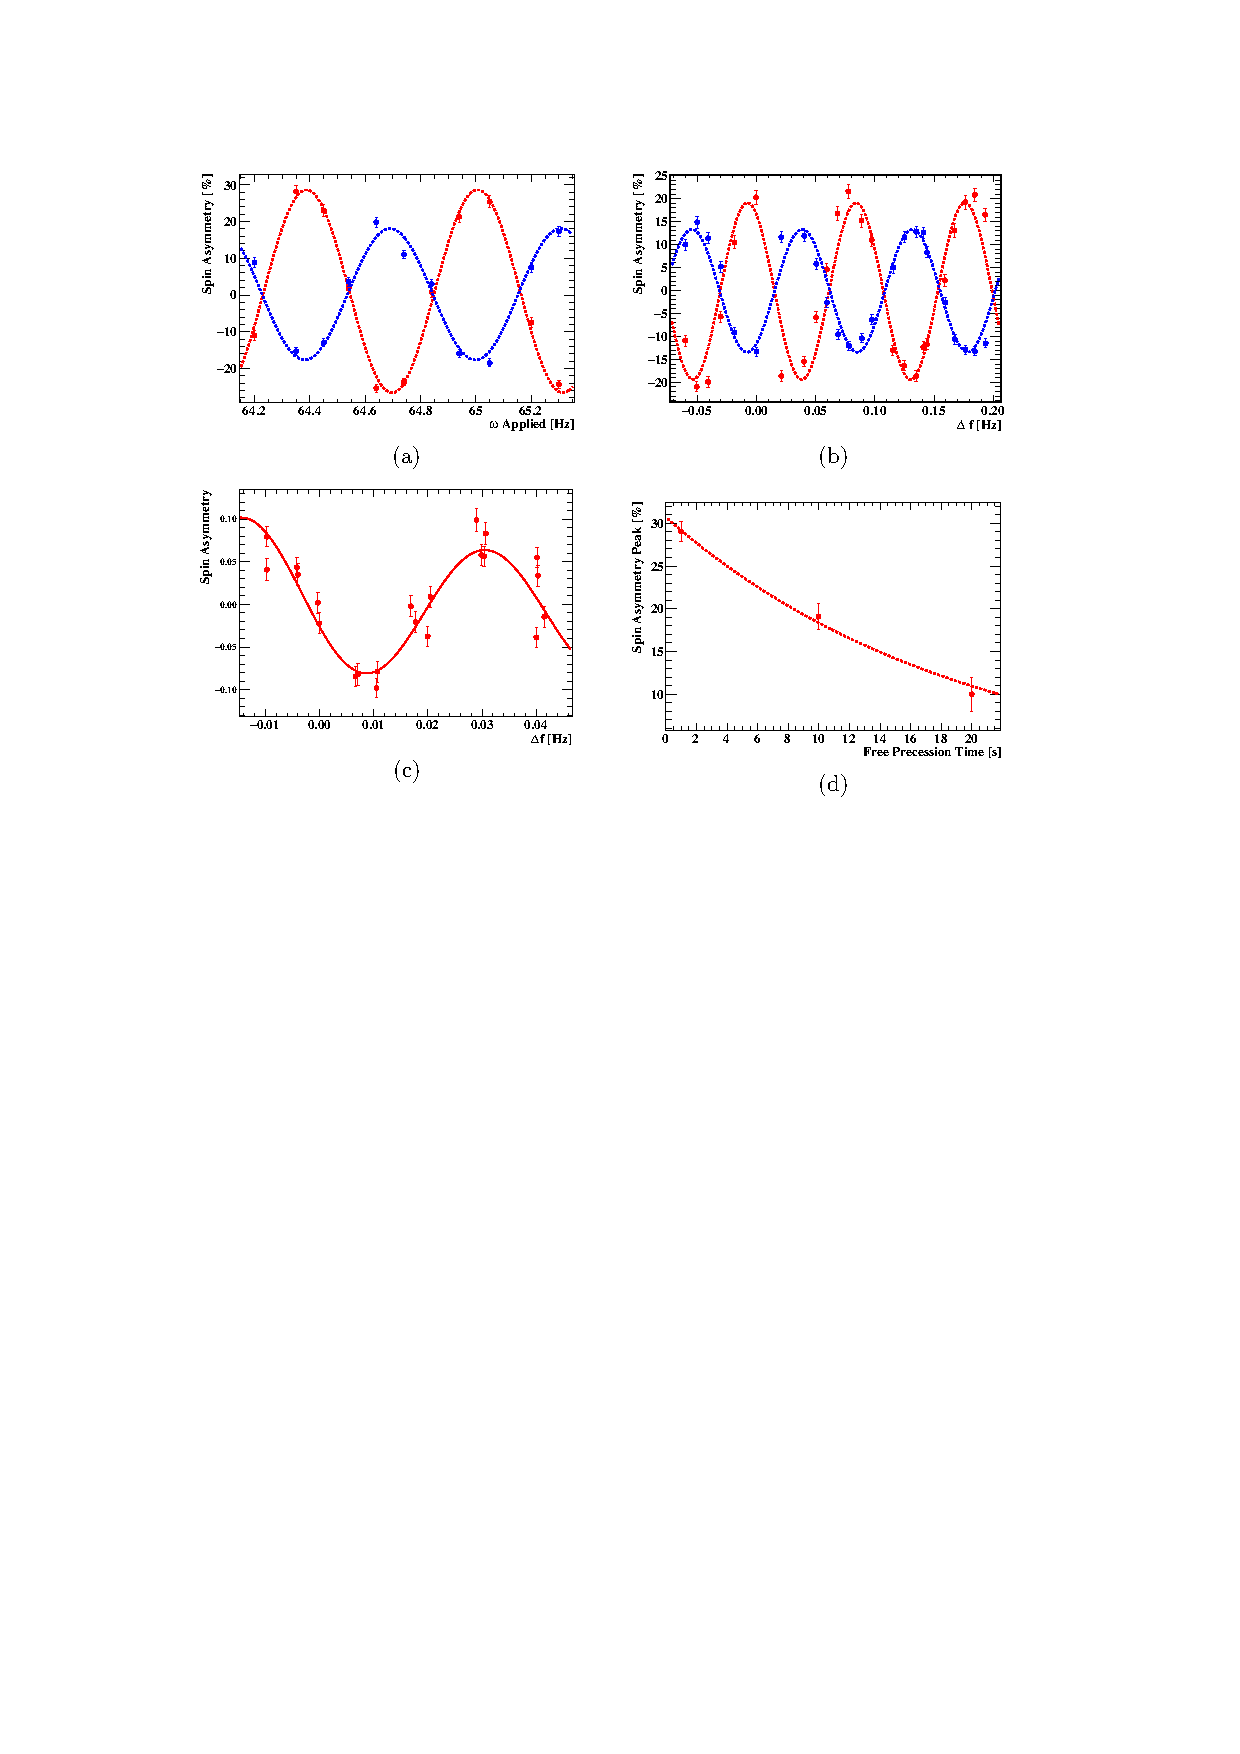
\includegraphics[width=\textwidth]{figures/2017_ramsey_fringes.pdf}
    \caption
    [Ramsey fringes measured in the prototype apparatus.]
    {Ramsey fringes measured in the prototype apparatus. Free precession period $\gls*{T_fp}=\text{\textbf{(a)} }\qty{1}{s}$, \text{\textbf{ (b)} }$\qty{10}{s}$, \text{\textbf{ (c)} }$\qty{20}{s}$. Panel \textbf{(d)} shows a fit to the maximal spin asymmetry of each fringe (\ref{eq:spin_asymmetry}) as a function of \gls*{T_fp}. A fit of \textbf{(d)} with a decaying exponential gives $T_2=19.5(2.7)\text{ s}$. Figures provided by Robert Pattie Jr. and Takeyasu Ito.}
    \label{fig:ramsey_fringes_2017}
\end{figure}
%%%%%%%%%%%%%%%%%%%%%%%%%%%%%%%%%%%%%%%%%%

\chapter{North beamline characterization}
\label{chap:north_beamline_paper}

%%%%%%%%%%%%%%%%%%%%%%%%%%%%%%%%%%%%%%%%%%

The content in this chapter is adapted from Ref.~\cite{wong_north_beamline_2023}. The measurements presented were taken in 2019 and 2020, prior to the construction of the large MSR in the experimental area.

We demonstrate successful instrumentation of a prototype precession cell, single-channel spin analyzer, spin flipper, UCN detector, and rotary switcher for UCN transport in preparation for the LANL nEDM experiment. Approximately 60,000 UCN, sufficient to obtain a statistical uncertainty of $\delta \gls*{d_n} = 2\times 10^{-27}$~$e\cdot\text{cm}$ for the nEDM have been stored in a prototype cell with dPS-coated PMMA walls and NiP-coated Al electrode plates. 

We also introduce an analytical model that provides a parametrization of the input UCN energy spectrum on the beamline. We have successfully applied this model to the analysis of a series of UCN storage curves taken with prototype precession cells of the LANL nEDM experiment and data on UCN transmission through the PM. The extracted UCN velocity spectrum can be used to analyze and optimize the performance of the LANL nEDM experiment. 

With the \ucn source upgrade at LANL (Sec.~\ref{sec:lanl_ucn_source}), a new UCN beamline (called the North Beamline) was constructed for the new nEDM experiment (Fig.~\ref{fig:AreaB_schematic}). As part of the commissioning of the North Beamline and development of the new nEDM experiment, we performed a series of UCN transport and storage measurements using a prototype nEDM precession cell. 

 The statistical uncertainty of a Ramsey sequence measurement is given by Eq.~(\ref{eq:figure_of_merit})
%
\begin{gather*}
    \sigma_{\gls*{d_n}} = \frac{\hbar}{2\gls*{alpha} E \gls*{T_fp} \sqrt{N}}
\end{gather*}
%
where $\hbar$ is Planck’s constant, \gls*{alpha} is a factor describing the spin contrast of a Ramsey fringe (\ref{eq:alpha}), $N$ is the number of detected UCN, and $E$ is the strength of the applied electric field. $N$ is affected by UCN density at the location of the experiment, a result of UCN source performance and UCN transport. Both $N$ and \gls*{T_fp} depend on the UCN storage property of the precession cell (i.e., how the number of stored UCN depends on the time over which UCN are stored in the precession cell), which is in turn affected by the input UCN energy spectrum as well as the wall loss properties of the cell. The operating condition (i.e., how long to load the cell, how long to store the UCN, and how long to unload the cell, etc) is optimized to minimize the uncertainty of the experiment. Therefore, the measurements described in this chapter were focused on characterizing the UCN density and energy spectrum at the location of the experiment, as well as the UCN storage property of the precession cell. 

%%%%%%%%%%%%%%%%%%%%%%%%%%%%%%%%%%%%%%%%%%

\section{\label{sec:northBeamlineSetup}Description of experimental setup (2019 and 2020)}

%%%%%%%%%%%%%%%%%%%%%%%%%%%%%%%%%%%%%%%%%%

The schematic diagram of the experimental setup mounted on the North Beamline (2019 and 2020) is shown in Fig.~\ref{fig:NorthBeamlineLayout}. There were two gate valves (\acrshort*{gv}) located on the beamline, with a \qty{6.35}{\mm}-diameter ``monitor port'' located in between. The rate of UCN through the monitor port is proportional to the UCN density in the guides. For an isotropic distribution the rate $R$ through the monitor port hole with an area $A$ and the UCN density $\rho$ are related via  $R = \frac{1}{4} \overline{v} \rho A$ (Appx.~\ref{appx:ucn_effusion}), where $\overline{v}$ is the average UCN speed, i.e. $\overline{v} = \int vf(v)dv$, with $f$ describing the UCN velocity distribution). Hence, the rate of the monitor detector gives the approximate density of the UCN in the guide.

Refer to Sec.~\ref{sec:PM_description} for a description of the superconducting polarizing magnet (\acrshort*{pm}) and PM window. For the measurements in this chapter, we varied the strength of the PM field $ |\gls*{bField} |$ for the purpose of obtaining information on the UCN spectrum.



\begin{figure}[htp]
    \centering
    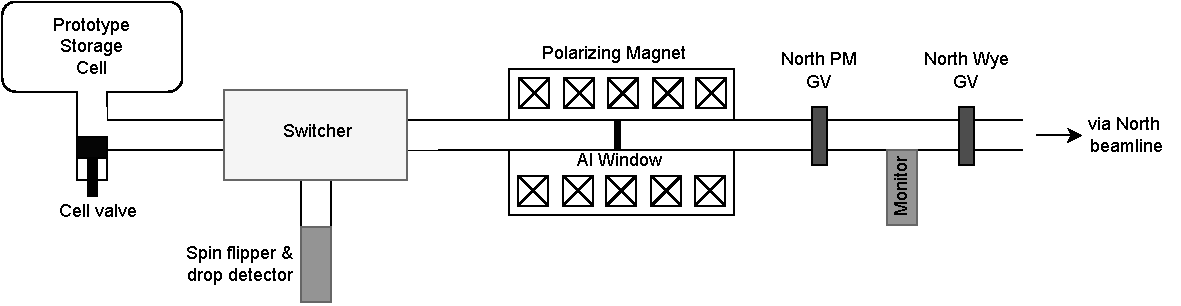
\includegraphics[width=14cm]{NorthBeamline.pdf}
    \caption[Layout of the North Beamline (2019 and 2020).]{Layout of the North Beamline (2019 and 2020). Two types of switchers were tested, see Sec.~\ref{sec:northBeamlineSetup} for description}
    \label{fig:NorthBeamlineLayout}
\end{figure}

A UCN switcher was located downstream of the PM. The switcher directed UCN from the source to the cell (fill mode) or from the cell to a UCN spin analyzer and detector (counting mode). In the counting mode, UCN were sent to a ``drop detector'' located below beam height. Two types of switchers were utilized for the measurements described in this paper. The first one was termed the ``prototype switcher,'' and the second, used for the LANL nEDM experiment, was termed the ``rotary switcher'' (Sec.~\ref{sec:lanl_switchers}).

The prototype switcher contains a guide segment that can be set to a straight-through position to fill the cell, or angled downward to send UCN from the cell to the drop detector. For the rotary switcher, the drop detector was connected via a downward bend attached to one of the guide ports. 

All guide sections downstream of the PM had a \qty{50}{\micro\meter}-thick electroless nickel phosphorus (NiP) coating. NiP has a high neutron optical potential (Sec.~\ref{sec:ucn_matter_int}) of \qty{213(5)}{\nano\eV}, a low spin-flip probability per bounce of $3.6(5) \times 10^{-6}$, and a low UCN loss probability per bounce of $1.3(1) \times 10^{-4}$ \cite{tang_measurement_2016, pattie_jr_evaluation_2017}. To adiabatically transport neutron spins, the guides downstream of the PM were kept under a $\sim\qty{1}{mT}$ magnetic field produced by coils.

On both the monitor and the drop detector, $\ce{^{10}B}$ coated ZnS:Ag scintillator films coupled with PMTs were used for UCN detection (Sec.~\ref{sec:ucn_detectors}). The photocathode diameters of the drop detector and monitor detector PMTs were \qty{76.2}{\mm} and \qty{28.6}{\mm}, respectively.

A neutron spin analyzer that consisted of a 10 layer polarizer~\cite{ThorstenThesis} made of iron and silicon was located immediately above the drop detector. Section~\ref{sec:spin_flipper_analyzer} includes a description of the apparatus and a discussion of the spin analyzing power of the system. We note that main conclusion of the results reported here does not depend on the exact value of the analyzing power, and use the value reported by Ref.~\cite{ThorstenThesis} of $99.3^{+0.7}_{-2.4}\%$.

UCN were stored in a prototype nEDM precession cell (Sec.~\ref{sec:precession_cells}). Several different configurations for the cell were used in the measurements for this paper and are discussed in further detail in Sec.~\ref{subsec:holdingTimeMeasurement}. The bottom of the cell was located approximately \qty{10}{\cm} above beamline guide height.

\begin{figure}
    \centering
    \includegraphics[width=0.6\textwidth]{exampleRun.pdf}
    \caption[UCN count rate during the ``fill-and-dump" measurement sequence for one run.]{UCN count rate during the ``fill-and-dump" measurement sequence for one run. Preload: \qtyrange{0}{100}{\s}. Filling period: \qtyrange{100}{150}{\s}. Holding period: \qtyrange{150}{330}{\s}. Counting period: \qtyrange{330}{430}{\s}.}
    \label{fig:timeSpectrum}
\end{figure}

\begin{figure}
    \centering
    \includegraphics[width=0.5\textwidth]{dummyCell.png}
    \caption[A photograph of a prototype precession cell]{A photograph of a prototype precession cell (pictured here with NiP-coated Al cell walls)}
    \label{fig:dummyCell}
\end{figure}

%%%%%%%%%%%%%%%%%%%%%%%%%%%%%%%%%%%%%%%%%%%%%%

\section{\label{sec:measurement}Measurements}

\subsection{\label{subsec:holdingTimeMeasurement}Measurement of UCN storage time}

%%%%%%%%%%%%%%%%%%%%%%%%%%%%%%%%%%%%%%%%%%%%%%

A UCN storage lifetime measurement was performed using a ``fill-and-dump" method. The steps were: (1)~The North Wye GV was opened while the North PM GV was kept closed for \qty{100}{\s} to ``preload" the UCN to build up UCN density behind the GV. (2)~The North PM GV was opened, allowing UCN to pass through the PM and the switcher into the cell. This filling period was \qty{50}{\s}. (3)~The cell valve and North PM GV were closed to stop the flow of UCN into the precession cell. (4)~The cell valve was kept closed for some ``holding time" to store UCN. (5)~The switcher moved from the fill mode to count mode in preparation to empty the cell. (6)~The cell valve was opened to allow UCN to flow to the drop detector. This counting period lasted for \qty{100}{\s}. Note that for these of measurements, the UCN final spin was not measured. See Fig.~\ref{fig:timeSpectrum} for the drop detector UCN count rate for one such run.

Two different types of cell side walls were tested: (i)~NiP coated Al and (ii)~deuterated polystyrene (dPS) coated poly(methyl methacrylate) (\acrshort*{pmma}). In both cases, the top and bottom surfaces of the cell were NiP-coated Al.  A photograph of the prototype cell is shown in Fig.~\ref{fig:dummyCell}. In the final nEDM experiment the dPS-coated PMMA cell side wall will be used in combination with top and bottom plates made of Al coated with a diamond-like carbon (\acrshort*{dlc}), which will be used as ground and high voltage electrodes. We used NiP coating, instead of DLC, for the reason that it was easier to obtain. However, given that DLC has a higher neutron optical potential~\cite{Atchison2006} than NiP and also given that the loss parameter we obtained for NiP was similar to that measured for DLC (see Sec.~\ref{sec:analysis}), a cell made of a dPS-coated PMMA side wall and the NiP coated plates provides conditions sufficiently close to the final nEDM experiment. To further approximate the condition of the final nEDM experiment, the top and bottom plates have a groove with rounded edges where the end of the insulating wall meets them, a feature needed to avoid enhanced electric fields (see, e.g. Sec. 3.3 of Ref.~\cite{cp_violation_wo_strangeness}).  

The seals between the side wall and the top and bottom plates were provided by an o-ring, located inside the groove mentioned above, minimizing the exposure to UCN. To ensure that the storage time was not affected by upscattering of UCN from residual gas, we maintained a storage volume vacuum of $10^{-5}$~Torr or better. A high voltage was not applied to the high voltage electrode (although it was possible when the side wall was the one made of dPS-coated PMMA), as it was not essential for the purpose of the measurement. As a result, the cell was placed in the atmosphere (as shown in Fig.~\ref{fig:dummyCell}) as opposed to in an insulating vacuum. 

Fill-and-dump holding time scans were repeated for holding times of 30 to 300 seconds. Holding time scans were repeated with PM strengths of \qtylist{0; 1.25; 2.5; 3.75; 5}{\tesla}. An overview of UCN hold-time run conditions is summarized in Tab.~\ref{tb:runconditions}. For run condition 1, the UCN source was run continuously and the GV was simply opened and closed between fill-and-dump measurements. To avoid delivering beam to the target unnecessarily, run conditions 2--4 switched to a mode where the beam was on only during preload and filling periods.

\begin{table}
\centering
\caption[North beamline characterization run conditions]{\label{tb:runconditions}Switcher, cell wall, and PM window conditions for measurements} 
\begin{tabular}{lll}
\toprule
\multicolumn{1}{l}{$\#$} & \multicolumn{1}{l}{Run Condition}  & \multicolumn{1}{l}{Storage Curve} \\
\midrule
 1 & Prototype switcher, NiP coated Al cell wall, no  PM window & Fig. \ref{fig:runCondition1_fit} \\  
 2 & Prototype switcher, NiP coated Al cell wall, with PM window & Fig. \ref{fig:runCondition2_fit} \\
 3 & Rotary switcher, NiP coated Al cell wall, with PM window & Fig. \ref{fig:runCondition3_fit} \\
 4 & Rotary switcher, dPS coated PMMA cell wall, with PM window & Fig. \ref{fig:runCondition4_fit} \\
\bottomrule
\end{tabular}
\end{table}

%%%%%%%%%%%%%%%%%%%%%%%%%%%%%%%%%%%%%%%%%%%%%%

\subsection{\label{subsec:PMrampMeasurement}Measurement of spin dependent UCN transmission rate as a function of PM field}

%%%%%%%%%%%%%%%%%%%%%%%%%%%%%%%%%%%%%%%%%%%%%%

Direct ``flow-through" measurements of UCN transmission through the PM were taken to provide information on the incoming UCN energy spectrum. During these measurements, the magnetic field of the PM was slowly decreased from \qtyrange{5}{0}{\tesla} or increased from \qtyrange{0}{5}{\tesla}, depending on the initial state of the PM. \qty{44}{\minute} are needed to ramp between 0~T and 4.11~T, and \qty{28}{\minute} to ramp between 4.11~T and 5.0~T, a total of \qty{72}{\minute}. UCN were transported from a continuously operated source to the drop detector, while the \acrshort{afp} spin flipper state was toggled every \qty{67}{\s}. The period of 67~s (= \qty{0.015}{Hz}) was chosen to ensure sufficiently frequent toggling between the two spin states while providing a long enough period for each segment of measurement needed for accurate analysis. These measurements were performed with the Al window installed in the PM region. Analysis of this data is presented in Sec.~\ref{subsec:PMramp}.

\begin{figure}
    \centering
    \includegraphics[width=0.6\textwidth]{preloadFit.pdf}
    \caption[An illustration of a preload fit used for normalization under run conditions 2--4, as described in section \ref{subsec:dataProcessing}.]
    {An illustration of a preload fit used for normalization under run conditions 2--4, as described in section \ref{subsec:dataProcessing}. Data in this figure is obtained from an upstream monitor located on the ``West Beamline''. UCN density is built up behind a stainless steel gate valve for \qty{100}{\s}. The gate valve is then opened to allow UCN to fill the precession cell on the north beamline, causing a dip on the upstream monitor rate}
    \label{fig:preloadFit}
\end{figure}

%%%%%%%%%%%%%%%%%%%%%%%%%%%%%%%%%%%%%%%%%%%%%%

\section{\label{sec:analysis}Data analysis and modeling}

\subsection{\label{subsec:dataProcessing}Data processing and normalization}

%%%%%%%%%%%%%%%%%%%%%%%%%%%%%%%%%%%%%%%%%%%%%%

In order to generate a reliable UCN storage time curve, it is necessary to subtract background and normalize UCN counts to correct for variations in UCN source intensity.

A monitor upstream of the PM located on the ``West Beamline" (see Fig.~\ref{fig:AreaB_schematic}) was used to normalize the number of UCN measured by the drop detector during the counting period. This monitor was chosen for normalization because the UCN source performance was characterized via West Beamline monitor before the addition of the North beamline. The West beamline monitor measured a UCN count rate of $\sim\qty{2000}{UCN \per s}$ (North PM GV closed) when beam and source parameters were optimally tuned. This monitor rate corresponded to a density of \qty{184(32)}{UCN\per\cm^3} at the exit of the biological shield (see Ref.~\cite{ito_performance_2018}).

The UCN rate measured in the West Beamline monitor as a function of time during the preload, $R(t)$, was fit to the form of an exponential, $R(t) = R_0( 1-\exp[-(t-t_0) /\tau ] )$, to determine free parameters $R_0,\,t_0,\text{ and } \tau$ for run conditions 2--4 in Tab. \ref{tb:runconditions}. The scaling factor to obtain a normalized UCN count is then given by $2000 / R(t=100\;{\rm s})$, the rate at the end of the preload period. An example of a preload fit utilized for normalization is illustrated in Fig.~\ref{fig:preloadFit}. For run condition 1, $R$ was taken to be the average value of the West Beamline monitor rate during the preload period because the beam was not turned off during the measurement run. The PMT background rate for each data set was fitted and subtracted from the UCN counting period.

During analysis, it was discovered that some portion of UCN storage runs had a small leakage of UCN during the storage period, a result of the cell valve not fully closing. Typically, in a leak-less run, UCN remaining in the guide system after the filling period drained into the drop detector in the first $\sim$~\qty{20}{\s} of the holding period. This ``guide-dump'' count of UCN could be fit with a single decaying exponential and typically exhibited a decay time on the order of one or two seconds. However, with a leak, a double exponential function was observed with a secondary decay on the order of $\sim$~\qty{50}{\s}. 

The leak-corrected count of UCN, $N_\text{cc}$, was obtained from the uncorrected count of UCN, $N_\text{c}$, with
%
\begin{gather}
    N_\text{cc} = N_\text{c} + \int^{t_2}_{t_1} dt \int^{t_3}_{t_2} dt'\, f(t)g(t') e^{-(t'-t)/\tau}\label{eq:leakCorrection}
\end{gather}
%
where, as illustrated in Fig.~\ref{fig:leakCorrection}, $t_1$ is the start of the holding period, $t_2$ is the start of the counting period, and $t_3$ is the end of the counting period. $N_\text{c}$ is obtained from the UCN counted during the counting period with background subtracted. The number of leaked UCN at a given time, $f(t)$, was obtained by fitting the guide dump on leak-free runs, and then subtracting the fit from runs with leaks. The rate of UCN detected at time $t$ during the counting period from the cell dump, $g(t)$, is normalized such that $\int g(t) dt = 1$.  The exponential term approximates the decay of stored UCN, where $\tau$ is the effective decay constant determined by fitting to the uncorrected storage curve.

The size of the leak correction varied. It was smaller for shorter holding time runs ($ < 2\%$ of counted UCN for storage times less than \qty{50}{\s}), and was larger for longer hold runs (up to 10\% of counted UCN for storage times of \qty{300}{\s}). The uncertainty of the leak correction was less than 5\% of the leak correction itself, as determined by taking into consideration all fitting and statistical uncertainties, making a negligible contribution to total measurement uncertainty. The normalized UCN counts thus obtained are plotted in Fig.~\ref{fig:runCondition1_fit}--\ref{fig:runCondition4_fit}.

\begin{figure}
    \centering
    \includegraphics[width=0.6\textwidth]{leakCorr}
    \caption[Visualization of parameters used for leak correction of UCN storage in Eq.~ (\ref{eq:leakCorrection})]{Visualization of parameters used for leak correction of UCN storage in Eq.~ (\ref{eq:leakCorrection}), as referred to in section \ref{subsec:dataProcessing}}
    \label{fig:leakCorrection}
\end{figure}

\begin{figure}
    \centering
    \includegraphics[width=0.75\textwidth]{Run_Condition_1_fit.pdf}
    \caption[UCN storage measurement run condition 1: Prototype switcher, NiP coated Al cell wall, no PM window.]{UCN storage measurement run condition 1: Prototype switcher, NiP coated Al cell wall, no PM window. Points with error bars represent data and curves represent fits. The $B=3.75$~T fit is suppressed due to overlap with the $B=5$~T curve. Fit results are described in Tab.~\ref{tb:fitResults}.}
    \label{fig:runCondition1_fit}
\end{figure}

\begin{figure}
    \centering
    \includegraphics[width=0.75\textwidth]{Run_Condition_2_fit.pdf}
    \caption[UCN storage measurement run condition 2: Prototype switcher, NiP coated Al cell wall, with PM Window.]{UCN storage measurement run condition 2: Prototype switcher, NiP coated Al cell wall, with PM Window. Points with error bars represent data and curves represent fits. The $B=1.25$~T, $B=2.5$~T and $B=3.75$~T fits are suppressed due to overlap with the $B=5$~T curve. Fit results are described in Tab.~\ref{tb:fitResults}.}
    \label{fig:runCondition2_fit}
\end{figure}

\begin{figure}
    \centering
    \includegraphics[width=0.75\textwidth]{Run_Condition_3_fit.pdf}
    \caption[UCN storage measurement run condition 3: Rotary Switcher, NiP coated Al cell wall, with PM window.]{UCN storage measurement run condition 3: Rotary Switcher, NiP coated Al cell wall, with PM window. Points with error bars represent data and curves represent fits. The $B=2.5$~T fit is suppressed due to overlap with the $B=5$~T curve. Fit results are described in Tab.~\ref{tb:fitResults}.}
    \label{fig:runCondition3_fit}
\end{figure}

\begin{figure}
    \centering
    \includegraphics[width=0.75\textwidth]{Run_Condition_4_fit.pdf}
    \caption[UCN storage measurement run condition 4: Rotary Switcher, dPS coated PMMA cell wall, with PM window.]{UCN storage measurement run condition 4: Rotary Switcher, dPS coated PMMA cell wall, with PM window. Points with error bars represent data and curves represent fits. The $B=1.25$~T, $B=2.5$~T and $B=3.75$~T fits are suppressed due to overlap with the $B=5$~T curve. Fit results are described in Tab.~\ref{tb:fitResults}}
    \label{fig:runCondition4_fit}
\end{figure}

%%%%%%%%%%%%%%%%%%%%%%%%%%%%%%%%%%%%%%%%%%%%%%

\subsection{\label{subsec:storageCurves}UCN storage curves in prototype precession cells}

%%%%%%%%%%%%%%%%%%%%%%%%%%%%%%%%%%%%%%%%%%%%%%

In this section we introduce an analytical model to fit UCN lifetime storage curves in the cell, with parameters that describe properties of the UCN storage vessel, physical parameters of the neutron velocity spectrum upstream of the PM, and the effect of the PM on the spectrum. This model can be used to quickly obtain physical information from UCN storage curves without the need to create a comprehensive Monte Carlo simulation of a system, which can be labor intensive and computationally costly.

It is a common practice to fit UCN storage lifetime measurements to single-exponential curves, which is only correct for a population of UCN with a single velocity and a single angle of incidence. However, both the velocity and angle have continuous distributions. Double exponential curves are often used to very approximately represent decay curves made of a two-component population including a super-barrier fraction. In cases where the UCN velocity spectrum affects the performance of the experiment, such as an nEDM experiment, a more sophisticated approach is in order. 

Let $dN_0/dv$ be the UCN velocity spectrum upstream of the PM, and $dN_1/dv$ be the UCN velocity spectrum downstream of the PM. As the starting point, for simplicity, assume the following functional forms:
%
\begin{align}
    \frac{dN_0}{dv} &\propto v^{\gls*{vspec}}\label{eq:dN0dv}\\ 
    \frac{dN_1}{dv} &= \frac{1}{2} \frac{dN_0}{dv} \left( f_h + f_\ell \right)\label{eq:dN1dv_noBeta}
\end{align}
%
where $\gls*{vspec}$ is a free parameter of the model. Equation~(\ref{eq:dN0dv}) is a functional form for the velocity distribution of the UCN as a result of the transport from the source to the location of the experiment, as utilized in Ref.~\cite{ito_performance_2018}. $f_h$ and $f_\ell$ are the fraction of high-field seekers and low-field seekers transmitted through the PM, respectively. The normalization of $f_h$ and $f_\ell$ is chosen such that $f_h=1$ and $f_\ell=1$ corresponds to the completely unpolarized case.  

In the situation with no window present in the center of the PM, the PM passes all the high field seeking neutrons with $v_\parallel>0$, where $v_\parallel$ is the longitudinal velocity along the axis of the UCN guide. The PM passes low field seeking neutrons for $v_\parallel>0$ only if
$\frac{1}{2}\gls*{m_n} \left( v_\parallel \right)^2 > \gls*{mu_n} B$, where \gls*{mu_n} is the neutron magnetic moment ($\gls*{mu_n}=$~\qty
{60}{\nano\eV\per\tesla}) \cite{codata_2018}. Let $v_{\text{c}\parallel}$ be the critical longitudinal velocity that fulfills this requirement, given by $v_{\text{c}\parallel} = \sqrt{2\gls*{mu_n} B/ \gls*{m_n}}$.

There is another factor that contributes to the transmission of UCN through the PM. If there is a spin-depolarizing region upstream of the PM (for example, we have gate valves made of stainless steel) and if the population of low-field seekers exceeds that of high-field seekers in the region upstream of the PM, which in turn is caused by low-field seekers being reflected by the PM potential (resulting in low $f_\ell$), there is a chance for low-field seekers to be spin-flipped and pass through the PM as high-field seekers. We can rewrite Eq.~(\ref{eq:dN1dv_noBeta}) as
%
\begin{align}
    \frac{dN_1}{dv} = \frac{1}{2} \frac{dN_0}{dv} \left[ f_h + f_\ell + \beta \left( f_h - f_\ell \right)  \right]
    \label{eq:dN1dv}
\end{align}
%
where $\beta$ is a free parameter (constrained to the range $[0,1]$) that describes this spin-flipping effect.

We now describe expressions for $f_h$ and $f_\ell$. For the no-window case we set $f_h = 1/2$, a value corresponding to the situation in which half of the UCN are directed upstream and half are directed downstream.  Strictly speaking, this holds only when the system has no loss. This condition is reasonably well met for the measurement of storage times (described in Sec.~\ref{subsec:holdingTimeMeasurement}) but is not at all met for the measurement of spin dependent UCN transmission (described in Sec.~\ref{subsec:PMrampMeasurement}) because in the latter case, all the transmitted neutrons are eventually detected. Nevertheless, this formalism is still valid because the backward flowing neutrons do not come into the picture and because there is an overall normalization constant $C$. It should be considered to be a choice of convention to set $f_h= 1/2 $ for no window case.


$f_\ell$ is a function of velocity that is dependent on the angular distribution of the UCN upstream of the PM and the strength of the PM field. For an isotropic angular distribution, the fraction of low field seekers allowed through the PM is
%
\begin{align}\label{eq:fL_isotropic}
    f_\ell &= \frac{2\pi \int^{\theta_\text{c}}_{0}\: d\theta \sin\theta}{4\pi} = \frac{1}{2}\left(1 - \cos\theta_\text{c}\right) \\
    &= \frac{1}{2}\left( 1 - \frac{v_{\text{c}\parallel}}{v} \right) \hspace{10pt} \text{ for } v>v_{\text{c}\parallel}
\end{align}
%
The limits of integration in the numerator were determined using the requirement $\cos\theta > v_{\text{c}\parallel} / v$ for low-field seeking neutrons.

As UCN are transported from the source to the experiment through the guide system, the angular distribution becomes more forward directed. For a completely forward directed population of low-field seekers, we have $f_\ell = 1/2 \text{ for } v>v_{\text{c}\parallel}$ and $f_\ell = 0$ otherwise. The angular distribution is likely to be somewhere in between. We write a more general expression for $f_\ell$ with a free parameter characterizing the angular distribution of low field seeking neutrons
%
\begin{gather}
    f_\ell=\frac{1}{2} \left( 1 - k\left(\frac{v_{\text{c}\parallel}}{v}\right) \right)  \hspace{10pt
    } \text{ for } v>v_{\text{c}\parallel}\label{eq:fL_k}
\end{gather}
%
where as $k$ approaches 0, the UCN velocity distribution becomes forward directed, and as $k$ approaches 1 the angular distribution becomes isotropic.

We now describe a set of equations that can be used to fit UCN storage curves in a precession cell
%
\begin{align}
    N(t) &= \int_{v_\text{low}}^{v_\text{high}} dv \frac{dN_1}{dv}\exp{\left(-\frac{t}{\tau(v',\overline{\mu})}\right)}\label{eq:holdingCurve_noWindowStart} \\
    \frac{1}{\tau(v',\overline{\mu})} &=\frac{1}{\tau_\beta}+\frac{Av'}{4\text{ Vol}}\overline{\mu} \label{eq:1overTau}\\
     \overline{\mu} &= 2\mu \left[ \frac{V_\text{cell}}{K(v')} \sin^{-1}\left( \frac{K(v')}{V_\text{cell}}\right)^{1/2} -\left( \frac{V_\text{cell}}{K(v')} - 1 \right)^{1/2} \right]\label{eq:lossPerBounce}\\
    \frac{dN_1}{dv} &= \frac{C}{2} v^{\gls*{vspec}} \left[ \frac{1}{2} + f_\ell + \beta \left( \frac{1}{2} - f_\ell \right)  \right] \label{eq:dN1dv_no_window}\\
    f_\ell &=\begin{cases}
        \frac{1}{2} \left( 1 - k\left(\frac{v_{\text{c}\parallel}}{v}\right) \right) \text{ for } v>v_{\text{c}\parallel} \text{ where } v_{\text{c}\parallel} = \sqrt{2 \gls*{mu_n} B/ \gls*{m_n}} \\
        0 \hspace{53pt}\text{otherwise}
        \end{cases}\label{eq:holdingCurve_noWindowEnd}
\end{align}
%
with free parameters $C$, $\mu$ (velocity-independent loss per bounce within the precession cell), $\beta$ (upstream depolarization probability), $\gls*{vspec}$ (velocity distribution), and $k$ (angular distribution). $N$ (without any subscripts) refers to the number of detected neutrons. 

The lower integration limit of Eq.~(\ref{eq:holdingCurve_noWindowStart}), $v_\text{low}$, is obtained from the gravitational potential $U$, the minimum energy of UCN required to enter a precession cell located above beam height.  The velocity of UCN that have entered the cell, $v'$, is related to $v$ by $v' = \sqrt{v^2 - 2U/ \gls*{m_n}}$. The term in the upper integration limit, $v_\text{high}$, is the velocity equivalent of $\min( V_\text{cell} + U,\, V_\text{guide})$, which is the maximum UCN energy from the input spectrum that is containable by either the transport guide (with neutron optical potential $V_\text{guide}$) or the precession cell (with neutron optical potential $V_\text{cell}$). Equation~(\ref{eq:1overTau}) describes the decay time of a stored UCN, which consists of the the free neutron lifetime $\tau_\beta$ with a velocity-dependent loss per bounce within the precession cell, where we assume that neutron velocity within the cell is isotropic. $A$ is the inner surface area of the precession cell, and Vol is the volume of the precession cell. Equation~(\ref{eq:lossPerBounce}), which describes loss per bounce, is taken from Eq.~2.70 in Ref.~\cite{golubUCN}, where $K(v')$ is the kinetic energy of the neutron in the cell. We assume that the UCN spectrum is not affected by the transport between the exit of the PM and the UCN precession cell. Therefore $dN_1/dv$ also represents the input UCN velocity spectrum of UCN in the guide that arrive at the cell.

The holding curve formalism described by Eqs.~(\ref{eq:holdingCurve_noWindowStart})--(\ref{eq:holdingCurve_noWindowEnd}) can also be modified to account for the presence of the Al window in the PM region. We maintain the base form of Eq.~(\ref{eq:dN1dv}), but now must alter our expressions for $f_\ell$ and $f_h$ to account for the step potential represented by the window, which for Al we approximate to be $V_\text{Al}=54\text{ neV}$ \cite{golubUCN}. Low-field seekers must now have a high enough velocity to overcome both the PM field potential and the Al window step potential. 

High-field seekers must also have a high enough velocity to overcome the window step potential, but receive the benefit of being accelerated by the PM field. When the energy increase from the PM field is greater than the neutron optical potential of the window, high-field seekers of any velocity are transmitted through the window.

To describe UCN storage curves with an Al window in the PM region, Eqs.~(\ref{eq:dN1dv_no_window}) and (\ref{eq:holdingCurve_noWindowEnd}) become
%
\begin{align}
     \frac{dN_1}{dv} &= \frac{C}{2}v^{\gls*{vspec}} \left[ f_h + f_\ell + \beta \left( f_h - f_\ell \right)  \right] \label{eq:dN1dv_window}\\
     f_\ell &=\begin{cases}
        \frac{1}{2} \left(1 - k \frac{v_{\text{c}\parallel}}{v} \right) \text{ for }  v>v_{\text{c}\parallel} \text{ where } \frac{1}{2}m \left(v_{\text{c}\parallel}\right)^2 = V_\text{Al} + \mu B\\
        0 \hspace{43pt} \text{otherwise}\end{cases}\\
    f_h &=\begin{cases}
        \frac{1}{2} \left(1 - k \frac{v_{\text{c}\parallel}}{v} \right) \text{ for } v>v_{\text{c}\parallel} \text{ where } \frac{1}{2}m \left(v_{\text{c}\parallel}\right)^2 = V_\text{Al} - \mu B \\ 
        \hspace{60pt} \text{and } V_\text{Al} > \mu B\\
        0 \hspace{40pt} \text{ for } v \leq v_{\text{c}\parallel} \text{ where } \frac{1}{2}m \left(v_{\text{c}\parallel}\right)^2 = V_\text{Al} - \mu B \\ 
        \hspace{60pt} \text{and } V_\text{Al} > \mu B\\
        \frac{1}{2} \hspace{40pt} \text{ for } V_\text{Al} \leq \mu B \label{eq:holdingCurve_windowEnd}  \end{cases}
\end{align}
%
This formalism enables a fit of both no-window and with-window UCN storage curves using the same set of free parameters.

%%%%%%%%%%%%%%%%%%%%%%%%%%%%%%%%%%%%%%%%%%%%%%

\subsection{\label{subsec:holdingCurveFits}Multi-parameter fits of UCN storage curves}

%%%%%%%%%%%%%%%%%%%%%%%%%%%%%%%%%%%%%%%%%%%%%%

Multi-parameter least square minimization fits were performed using the LMFIT Python library \cite{newville_matthew_2014_11813}. The results are presented in Tab.~\ref{tb:fitResults}. Data points were weighted using the total measurement uncertainty during the fitting process. For measurements with no window in the PM region, we fit Eqs.~(\ref{eq:holdingCurve_noWindowStart})--(\ref{eq:holdingCurve_noWindowEnd}), and for the measurements with a window present we fit Eqs.~(\ref{eq:holdingCurve_noWindowStart})--(\ref{eq:lossPerBounce}) and (\ref{eq:dN1dv_window})--(\ref{eq:holdingCurve_windowEnd}). It should be noted that the bottom of the prototype cell was located \qty{10}{\cm} above beam height. Therefore for NiP-coated Al wall run conditions we used an integration limits $v_\text{low}$ and $v_\text{high}$ as determined by $U=10$~\unit{\nano\eV} and $V_\text{guide} = 213$~\unit{\nano\eV} \cite{pattie_jr_evaluation_2017}. For dPS-coated PMMA wall run conditions we used $U=10$~\unit{\nano\eV} and $V_\text{cell} =160$~\unit{\nano\eV}.

For run condition 4,  we used a single effective loss per bounce parameter $\mu$ even though the cell was made of two different materials (i.e. dPS-coated cell wall with NiP electrodes). The reason for this was because the data did not have the sensitivity to resolve two separate $\mu$ values. This also applies to the simultaneous fit for data from run conditions 3 and 4. 

% https://www.tablesgenerator.com/
% Also, interesting link on table formatting 
% https://tex.stackexchange.com/questions/432770/fitting-my-table-into-tex-width-in-elsarticle
\begin{table}[ht]
\centering
\caption[Multi-parameter fits of UCN storage curves]{\label{tb:fitResults}Multi-parameter fits of UCN storage curves. Refer to Tab. \ref{tb:runconditions} for run condition details.}
\begin{tabular}{
l
S
S
S
S
c
c}
\toprule
Run					& 1				& 2				& 3				& 4				& \multicolumn{2}{c}{3 \& 4}							\\
\midrule
$C/10^3$			& 2(1)			& 3(1)			& 5(3)			& 5(3)			& \multicolumn{1}{c}{$4(1)$} & $7(2)$					\\
$\gls*{vspec}$			& 3.0(3)		& 2.5(2)		& 2.5(3)		& 2.7(2)		& \multicolumn{2}{c}{$\phantom{-}2.6(2)$}				\\
$\beta$				& 0.30(2)		& 0.8(2)		& 0.6(3)		& 0.8(2)		& \multicolumn{2}{c}{$\phantom{-}0.77(17)$}				\\
$k$					& 0.3(1)		& 0.6(1)		& 0.7(1)		& 0.5(1)		& \multicolumn{2}{c}{$\phantom{-}0.6(1)$}				\\
$\mu/10^{-4}$		& 2.0(1)		& 2.6(2)		& 3.5(4)		& 3.1(2)		& \multicolumn{2}{c}{$\phantom{-}3.4(2)$}							\\
Corr$(C,\gls*{vspec})$		& -1			& -0.94			& -0.96			& -0.96			& \multicolumn{1}{c}{$-0.97$}				& $-0.96$	\\
Corr$(C,\beta)$		& -0.2			& -0.32			& -0.4			& -0.5			& \multicolumn{1}{c}{$-0.49$}				& $-0.53$	\\
Corr$(C,k)$			& -0.7			& -0.14			& -0.14			& 0.02			& \multicolumn{1}{c}{$-0.16$}				& $-0.12$	\\
Corr$(C,\mu)$		& 0.9			& 0.85			& 0.77			& 0.79			& \multicolumn{1}{c}{$\phantom{-}0.78$}		& $\phantom{-}0.76$	\\
Corr$(\gls*{vspec},\beta)$	& -0.2			& 0.01			& 0.15			& 0.27			& \multicolumn{2}{c}{$\phantom{-}0.23$}					\\
Corr$(\gls*{vspec},k)$		& 0.71			& 0.44			& 0.37			& 0.22			& \multicolumn{2}{c}{$\phantom{-}0.41$}					\\
Corr$(\gls*{vspec},\mu)$	& -0.97			& -0.92			& -0.84			& -0.83			& \multicolumn{2}{c}{$-0.82$}							\\
Corr$(\beta,k)$		& -0.33			& -0.86			& -0.81			& -0.83			& \multicolumn{2}{c}{$-0.72$}							\\
Corr$(\beta,\mu)$	& 0.21			& 0.14			& 0.16			& -0.03			& \multicolumn{2}{c}{$\phantom{-}0.01$}					\\
Corr$(k,\mu)$		& -0.6			& -0.56			& -0.63			& -0.41			& \multicolumn{2}{c}{$-0.57$}							\\
Corr$(C_3,C_4)$		& 				& 				& 				& 				& \multicolumn{2}{c}{$\phantom{-}1\phantom{.00}$}		\\
\bottomrule
\end{tabular}
\end{table}

%%%%%%%%%%%%%%%%%%%%%%%%%%%%%%%%%%%%%%%%%%%%%%

\subsection{\label{subsec:PMramp}Spin dependent UCN rate as a function of the polarizing magnet field}

%%%%%%%%%%%%%%%%%%%%%%%%%%%%%%%%%%%%%%%%%%%%%%

A flow-through measurement as described in Sec.~\ref{subsec:PMrampMeasurement} was taken to obtain information on the input UCN spectrum. The switcher was set to channel polarized UCN from the PM directly into the spin analyzer and detector. For the duration of the measurement, the strength of the PM was slowly decreased from 5~T to 0~T and the spin flipper was toggled on and off at regular intervals (as per Sec.~\ref{subsec:PMrampMeasurement}). The Al window was present in the PM region for this measurement.

The flow-through measurement provides two curves describing neutron rate for each spin state as a function of the PM field strength (see Fig.~\ref{fig:pmRampFit}). These curves can be fit using the formalism described in Sec.~\ref{subsec:holdingCurveFits} with modification to account for finite efficiency of the spin analyzer and spin flipper.

Dividing Eq.~(\ref{eq:dN1dv_window}) into expressions for low-field seekers and high-field seekers
%
\begin{align}
\frac{dN_{1,\ell}}{dv} &= \frac{C}{2}v^{\gls*{vspec}} f_\ell = \frac{1}{2}v^{\gls*{vspec}} f_{\ell D}\\
\frac{dN_{1,h}}{dv} &= \frac{C}{2}v^{\gls*{vspec}} \left[ f_h + \beta \left( f_h - f_\ell \right)  \right] = \frac{1}{2}v^{\gls*{vspec}} f_{h D}
\end{align}
%
where $f_{\ell D} = f_\ell$ and $f_{h D} = f_h +  \beta \left( f_h - f_\ell \right)$  describe the fraction of low-field seekers and high-field seekers downstream of the  PM, respectively.

For spin analyzing power $\varepsilon_A$, when the spin flipper is off, there is some fraction of low-field seekers that are transmitted by the analyzing foil. Assuming that there is a negligible chance of depolarization downstream of the PM, the spectrum of the detected UCN with the spin flipper off is given by
%
\begin{gather}
    \frac{dN_\text{off}}{dv} = \frac{C}{2} v^{\gls*{vspec}} \left[ \varepsilon_A\, f_{h D} + (1-\varepsilon_A)f_{\ell D}  \right]
    \label{eq:dN_off/dv}
\end{gather}

When the spin flipper is on, for spin flipping efficiency $\varepsilon_S$, the spectrum of the detected UCN is
%
\begin{align}
    \frac{dN_\text{on}}{dv} &= \frac{C}{2} v^{\gls*{vspec}} \big[ \varepsilon_A\,\varepsilon_S\, f_{\ell D} + \varepsilon_A(1 - \varepsilon_S) f_{h D} \nonumber \\
    &\quad + (1 - \varepsilon_A)\varepsilon_S\,f_{h D}  + (1 - \varepsilon_A)(1-\varepsilon_A)\,f_{\ell D} \big]\label{eq:dN_on/dv}
\end{align}

In the above equation, the first term describes low-field seekers downstream of the PM that are successfully spin flipped to high-field seekers and allowed through the spin analyzer. The second term is the fraction of high-field seekers that were not flipped and allowed through the spin analyzer. The third term is the fraction of high-field seekers that were flipped to low-field seekers, but allowed through to the detector due to finite analyzing power of the foil. The fourth term is the fraction of low-field seekers that were not spin flipped, but allowed through the spin analyzer due to finite analyzing power.

Following Ref.~\cite{ThorstenThesis}, we assume a spin analyzing power of $\varepsilon_A=0.99$ for UCN in the energy range of the LANL nEDM experiment and a magnetized iron foil spin analyzer. Spin flipping efficiency $\varepsilon_S$ can be estimated as follows. With UCN in a flow-through mode from the source to the detector and with the PM at \qty{5}{\tesla}, when the spin flipper was turned on, detected UCN rate was reduced to $12\%$ compared to when the spin flipper was off (Fig.~\ref{fig:spin_flipper_efficiency}), which corresponds to the ratio of Eq.~(\ref{eq:dN_on/dv}) to Eq.~(\ref{eq:dN_off/dv}). Assuming negligible depolarization downstream of the PM, this means $f_{\ell D} = 0$ and $f_{hD} = 1/2$. Letting $\varepsilon_A=0.99$ and solving for $\varepsilon_S$ yields a spin flipping efficiency of $\varepsilon_S=0.89$.

The spin-flipper-off and spin-flipper-on curves were fit using an integral of $dN_\text{off}/dv$ and $dN_\text{on}/dv$, respectively, with limits of integration from \qtyrange{0}{7.58}{\meter\per\s} (the velocity equivalent of UCN in a \qty{5}{\tesla} field). This fit is shown in Fig.~\ref{fig:pmRampFit}, with the fit parameters from Tab. \ref{tb:pmRampFit}. 


\begin{table}
\centering
\caption{\label{tb:pmRampFit}Multi-parameter fit of a PM ramp}
\begin{tabular}{llllll}
\toprule
\multicolumn{1}{l}{Run condition} & \multicolumn{1}{l}{$\gls*{vspec}$} & \multicolumn{1}{l}{$\beta$} & \multicolumn{1}{l}{$k$} \\ 
\midrule
With Al window, UCN-flow through mode           & 1.0(1)      & 0.00(5)                 & 0.30(2)   \\
\bottomrule
\end{tabular}
\end{table}


\begin{figure}[htp]
    \centering
    \includegraphics[width=0.6\textwidth]{pmRampFit.pdf}
    \caption[A measurement of neutron transmission from the source to the drop detector with the B field of the PM decreasing from 5 T to 0 T over the course of 72 minutes, with the spin flipper toggling on and off.]{A measurement of neutron transmission from the source to the drop detector with the B field of the PM decreasing from 5 T to 0 T over the course of 72 minutes, with the spin flipper toggling on and off. This generates two curves that are describable using Eqs.~(\ref{eq:dN_off/dv}) and (\ref{eq:dN_on/dv}), which share the same set of free parameters as Eqs.~(\ref{eq:holdingCurve_noWindowStart})--(\ref{eq:lossPerBounce}) and  (\ref{eq:dN1dv_window})--(\ref{eq:holdingCurve_windowEnd}). The results of a simultaneous fit of these PM ramping curves are listed in Tab.~\ref{tb:pmRampFit}}
    \label{fig:pmRampFit}
\end{figure}

%%%%%%%%%%%%%%%%%%%%%%%%%%%%%%%%%%%%%%%%%%%%%%

\section{\label{sec:north_beamline_discussion}Discussion}

%%%%%%%%%%%%%%%%%%%%%%%%%%%%%%%%%%%%%%%%%%%%%%

As measured in run condition 4, Fig.~\ref{fig:runCondition4_fit}, a storage time of \qty{180}{\s} in a single cell yields a UCN count of $\sim60,000$ UCN, well in excess of the number required to reach the desired statistical uncertainty. In Ref.~\cite{ito_performance_2018}, $\gls*{alpha}=0.8$, $E=$~\qty{12}{\kilo\volt\per\cm}, $\gls*{T_fp}=$\qty{180}{\s}, $N=39,000$ for each cell, and $T_{\rm cycle} =$~\qty{300}{\s} were assumed to arrive at an estimated statistical uncertainty of $\sigma_{\gls*{d_n}}=4.0\times 10^{-26}e\cdot\text{cm}$ per day with a double cell geometry. With an assumed data taking efficiency of 50\% and the nominal LANSCE accelerator running schedule, this corresponds to a statistical uncertainty of $\sigma_{\gls*{d_n}}=2.1\times 10^{-27}e\cdot\text{cm}$ in 5 calendar years (Sec.~\ref{sec:lanl_nedm_uncertainty}). The number of stored polarized UCN observed was about 50\% larger than what was reported in a similar measurement performed on the West Beamline~\cite{ito_performance_2018}. We attribute the improvement to the better switcher transmission in spite of the longer transport distance. 

In the envisioned LANL nEDM experiment, two precession chambers will need to be filled. We expect that the achievable stored UCN density in the precession chambers will be minimally affected by going from one cell, as was done in this commissioning experiment, to two cells. In general, the ultimate achievable density in a volume that is made of several sections is given by $\rho = P/(\Sigma_i V_i/\tau_i)$, where $P$ is the UCN production rate (or a rate at which UCN enter the volume), $V_i$ is the volume of a section in which UCN has a lifetime $\tau_i$.  The volume of our system is dominated by the volume of the guide that transports UCN from the source to the experiment. As a result, we estimate the reduction in the achievable density due to the additional volume of the second cell and the associated guide to be up to 10\%. 

Additionally, we have demonstrated the utility of a UCN storage curve model. Varying the strength of the PM for UCN storage curves allowed the properties of a continuous UCN input energy spectrum on the North Beamline to be obtained. Importantly, the model describes both window-in and window-out storage with the same input parameters. The model is able to describe the unintuitive feature of the window-in run condition curves, where as the PM field increases in strength the normalized counts also increase. This behavior was the primary motivation for the introduction of the free parameter $\beta$ during analysis. For small $\beta$ (closer to 0) the model predicts that the number of UCN decreases as PM strength increases, but for larger $\beta$, low field seekers are spin-flipped and may pass through the PM region as a high field seeker, resulting in the behavior observed in Fig.~\ref{fig:runCondition2_fit}--\ref{fig:runCondition4_fit}.

We can draw a number of observations from the results of the UCN storage curves fits depicted in Tab.~\ref{tb:fitResults}. First, the value of $C$ in run conditions 3 and 4 is larger than the value in run condition 2, showing that the new rotary switcher transports a larger number of UCN than the old prototype switcher. Second, $k$ (ranging from 0.3(1) to 0.7(1)) across all run conditions indicates that the angular distribution of the input UCN velocity spectrum on the beamline is relatively forward directed. Third, $\beta$ is $\sim 0.7$ for run conditions with the Al window and is $\sim 0.3$ for the run condition without the window. This is consistent with the idea that the presence of the Al window reduces the number of low-field seeking UCN that pass the PM region, resulting in an increased chance for a low-field seeker to see a depolarizing region upstream of the PM and an effectively larger $\beta$. Comparatively, in the no window case, more low-field seekers pass the PM region, lowering the chance for a low-field seeker to be spin-flipped and giving a smaller value for $\beta$. 

In some cases there are rather large correlations among parameters as seen in Tab.~\ref{tb:fitResults}. The largest parameter correlations for fits across all run conditions are  $\text{Corr}(C,\gls*{vspec}) \sim -1$, $\text{Corr}(\gls*{vspec},\mu) \sim -0.9$, and $\text{Corr}(C,\mu) \sim 0.8$. Special care was taken in the least-squares fitting process to choose initial parameter guesses for $\gls*{vspec}$ and $\mu$ that were based on previous measurements along the West Beamline (see Ref.~\cite{ito_performance_2018, pattie_jr_evaluation_2017}) because of these correlations. As a result, we obtained $\gls*{vspec} \sim 3$ and $\mu \sim 3\times 10^{-4}$ across all run conditions, where $\gls*{vspec}$ was constrained to the range $[1,5]$ and $\mu$ was constrained to the range $[10^{-3}, 10^{-5}]$ during fitting. These values are consistent with previously measured values of $\mu = 1.4(2)\times 10^{-4}$ (Ref.~\cite{pattie_jr_evaluation_2017}) and $\gls*{vspec} = 2.9(0.6)$ (Ref.~\cite{ito_performance_2018}).

It can be seen in Fig.~\ref{fig:runCondition1_fit} that the storage curve model reproduces the storage curves at each PM field strengths for configurations without a window. For configurations with a window in the PM region (Fig.~\ref{fig:runCondition2_fit}--\ref{fig:runCondition4_fit}), the holding curve model reproduces the storage curves for holding times less than \qty{200}{\s}. For longer holding times ($>$~\qty{200}{\s}) in run conditions with the PM window, the holding curve model overpredicts the number of UCN. This is especially apparent in Fig.~\ref{fig:runCondition2_fit}, for holding times of \qty{500}{\s} for $B=3.75\text{ T}$ and $B=2.5\text{ T}$, as well as the $B=0\text{ T}$ and $B=1.25\text{ T}$ curves for holding times greater than \qty{200}{\s}. 

The statistical and leak correction uncertainties for longer holding time data points are too small to attribute the overprediction purely to weighting of the data points during the fitting process. In addition, the model is able to describe the behavior of the curves in run condition 1 for all PM field strengths.  We postulate that there is an additional mechanism caused by the presence of the window that preferentially selects for higher energy UCN to enter the precession cell. Higher energy UCN experience more wall collisions within the precession cell and have a higher loss per bounce, increasing the chance to be lost during the storage period.

One possible mechanism is bulk scattering of UCN within the PM window caused by nonuniformities within the window material. The magnetic field accelerates high-field seeking UCN through the Al window. If the window scatters the UCN, then a fraction of the longitudinal velocity (i.e. along the direction of the beamline) results in a transverse velocity component. Lower energy UCN may lose enough longitudinal velocity and become trapped in the the PM field potential well, a process less likely for higher energy UCN.

Lastly, we have shown that elements of the holding curve model may be adapted to a UCN flow-through measurement through a PM with an Al window, while the PM slowly ramps up or down. We observe that the model is able to reproduce the major features of the data (Fig.~\ref{fig:pmRampFit}). As the B field increases, low-field seekers are reflected by the potential well of the PM. Conversely, the fraction of high field seekers allowed past the Al window slowly increases with the strength of the B field, until the strength of the B field reaches a threshold where all high-field seekers are accelerated past the window region. The parameters of the model, presented in Tab. \ref{tb:pmRampFit}, indicate a forward-directed angular distribution ($k=0.30(2)$) consistent with the holding curve fits in Tab. \ref{tb:fitResults}. The estimate of $\beta=0$ is also consistent with what we expect, because UCN in a flow-through measurement with no preload period have less opportunity to be spin-flipped upstream of the PM.

The precision for $\gls*{vspec}$ in Tab. \ref{tb:pmRampFit} is limited due the change in the UCN energy spectrum during the course of the flow-through measurement. During the \qty{72}{\minute} period required to ramp the PM, the continuous use of the UCN source causes heating and a corresponding change in the input energy spectrum \cite{anghel_solid_2018}. Note that the measurement depicted in Fig.~\ref{fig:pmRampFit} was a PM ramp down sequence, where the field was decreased from \qtyrange{5}{0}{\tesla}. Since there is no time dependence for $\gls*{vspec}$, the model is less descriptive of the data obtained near the end of the ramp (\qtyrange{1}{0}{\tesla}).


%%%%%%%%%%%%%%%%%%%%%%%%%%%%%%%%%%%%%%%%%%

\chapter{Testing of components on the West beamline}\label{chap:fall2021}

%%%%%%%%%%%%%%%%%%%%%%%%%%%%%%%%%%%%%%%%%%

\begin{figure}
\centering
%subfigure width gets "multiplied" by includegraphics width
\begin{subfigure}{.5\textwidth} 
  \centering
  \includegraphics[width=\textwidth]{figures/west_beamline_switcher_tests.png}
  \caption{}\label{subfig:west_beamline_switchers}
\end{subfigure}%DO NOT REMOVE THIS '%'
\begin{subfigure}{.5\textwidth}
  \centering
  \includegraphics[height=3in]{figures/switcher_mockup.png}
  \caption{}\label{subfig:switcher_mockup}
\end{subfigure}
\caption
{Caption}
\label{fig:west_beamline_switchers}
\end{figure}

% Both PMTs beam height on switcher 1 (higher switcher)
% ======================================================
% SINGLE CHANNEL DET FOIL OUT
% detector rate: 1443.88
% wgv rate: 632.46
% normalized to wgv 650 [Hz]: 1483.9230939506056

% BEAM HEIGHT DET: WEST TEST PORT
% detector rate: 1435.18
% wgv rate: 641.26
% normalized to wgv 650 [Hz]: 1454.7406668122135

% BEAM HEIGHT DET: STRAIGHT THROUGH
% detector rate: 1498.215
% wgv rate: 635.39
% normalized to wgv 650 [Hz]: 1532.6645839563103

% Beam height PMTs on both switchers
% ======================================================
% SINGLE CHANNEL DET FOIL OUT
% detector rate: 1465.2666666666667
% wgv rate: 656.6
% normalized to wgv 650 [Hz]: 1450.5381256980404

% BEAM HEIGHT DET: SWITCHER 2 (LOWER)
% detector rate: 2244.225
% wgv rate: 650.0416666666666
% normalized to wgv 650 [Hz]: 2244.0811486443176

% BEAM HEIGHT DET: SWITCHER 1 (HIGHER)
% detector rate: 1512.1142857142856
% wgv rate: 649.5142857142857
% normalized to wgv 650 [Hz]: 1513.2450622443143

% Switcher 2 transmission difference: 1.5425987599300384
%%%%%%%%%%%%%%%%%%%%%%%%%%%%%%%%%%%%%%%%%%

\chapter{Commissioning of the nEDM apparatus}\label{chap:nEDM_commissioning_dec2022}

%%%%%%%%%%%%%%%%%%%%%%%%%%%%%%%%%%%%%%%%%%
%%%%%%%%%%%%%%%%%%%%%%%%%%%%%%%%%%%%%%%%%%

\chapter{Monte carlo simulations of UCN transport and spin transport}\label{chap:simulations}

%%%%%%%%%%%%%%%%%%%%%%%%%%%%%%%%%%%%%%%%%%

%%%%%%%%%%%%%%%%%%%%%%%%%%%%%%%%%%%%%%%%%%

\section{PENTrack}

%%%%%%%%%%%%%%%%%%%%%%%%%%%%%%%%%%%%%%%%%%

Arbitrary STL files, define material types based on real and imaginary potentials. Numerical or analytical fields (time dependent) both supported. Specularity can be lambertian or based on micro roughness \ref{sec:diffuse_reflections}. Supports \hg, xenon, electrons, protons, etc. Spin tracking works even at higher velocities due to relativistic spin equations \ref{sec:BMT_equations}. ODE integration method is a 5th order Dortmund Prince from the BOOST cpp library. \cite{schreyer_pentrack}

%%%%%%%%%%%%%%%%%%%%%%%%%%%%%%%%%%%%%%%%%%

\subsection
{
    \texorpdfstring{PENTrack on the Carbonate cluster at \acrshort{iu}}
                    {PENTrack on the Carbonate cluster at IU}
}

%%%%%%%%%%%%%%%%%%%%%%%%%%%%%%%%%%%%%%%%%%

PENTrack seeding/clock cycle system. PENTrack cluster scripts appendix

%%%%%%%%%%%%%%%%%%%%%%%%%%%%%%%%%%%%%%%%%%

\section{Simulation of UCN rate change from switcher height differential}

%%%%%%%%%%%%%%%%%%%%%%%%%%%%%%%%%%%%%%%%%%

%%%%%%%%%%%%%%%%%%%%%%%%%%%%%%%%%%%%%%%%%%

\section{Simulation of transport from the UCN source into the apparatus}

%%%%%%%%%%%%%%%%%%%%%%%%%%%%%%%%%%%%%%%%%%

%%%%%%%%%%%%%%%%%%%%%%%%%%%%%%%%%%%%%%%%%%

\section{1D random walk}\label{sec:1D_random_walk}

%%%%%%%%%%%%%%%%%%%%%%%%%%%%%%%%%%%%%%%%%%

The probability for a neutron to be lost in the bulk of the aluminum window in a single pass can be described by

\begin{gather}
   P_\text{abs} = 1 - \exp \left( - \frac{\ell_\text{window} }{ \ell_\text{mfp} } \right)
\end{gather}

where $\ell_\text{window}$ is the thickness of the window (0.003 in. \comment{clearly wrong}), and $\ell_\text{mfp} = 1 / (N\sigma_\text{abs})$ is the mean free path of absorption. $N$ is number density and $\sigma_\text{abs}$ is the velocity-dependent neutron absorption cross section of the material. 

It should be noted that high-field seeking UCN gain approximately 300 neV from the PM field, so neutrons that encounter the window will be in the 300 neV to 515 neV regime. $P_\text{abs}$ can be approximated as 0.03 for this energy range. This single pass loss probability is lower than the observed value of ($10.3\pm 2.8$)\% described in section subsec:windowLoss. However, nonspecularity of the UCN transport pipe can lead UCN to pass through the window region multiple times, increasing transmission loss. 

The loss from multiple window passes is estimated using a simple monte carlo simulation, where neutron transmission into the precession chamber is modeled as a 1D random walk. Each step in the random walk corresponds to the distance traveled between non-specular bounces. 

From eq. 4.79, eq. 4.70, and eq. 4.48 in reference \cite{golubUCN}, we write the step size between non-specular bounces as

\begin{gather}
    L_\text{spec} = 2 R\sqrt{\frac{2(2-d)}{3d} }
\end{gather}


where $R$ is the radius of the cylinder and $d$ is the chance for a diffuse bounce

Nonspecularity is approximately 0.05 for NiPh pipes (as measured by Ref. \cite{pattie_jr_evaluation_2017}). {\color{blue}Guide is stainless steel coated in NiPh, we know nonspecularity of stainless steel tubing (find manufacturer spec). Maybe Andy's paper. Adding NiPh may increase nonspecularity by a few percent. Basically it's a free parameter} therefore we let $N_\text{specular bounces} = 20$. For a pipe ID of 3 inches and total pipe length of 12 meters, step size = 0.75 meters.

Neutrons that return to the source are considered lost and removed from simulation. We also assume that neutrons which make it to the chamber do not leave

When a neutron reaches the end of the 1D pipe, the odds of it getting into the cell is modeled as

\begin{align}
    \text{cellChance} &= \left(1 - \left( 1 - \frac{ \text{openingArea} } {\text{total inner surface area of last segment}} \right) ^ {N_\text{spec}} \right)^2 \\
    &= \left(1 - \left( 1 - \frac{ (\text{cellEntranceID}/2)^{2} } {\text{pipeID}\times\text{step size}} \right) ^ {N_\text{spec}} \right) ^2 \\
    &\approx \left( \frac{ (\text{cellEntranceID}/2)^{2} \times N_\text{spec} } {\text{pipeID}\times\text{step size}} \right)^2
\end{align}

There is an extra factor of 2 because a nonspecular ``rejection'' step gives the neutron a second chance to enter the chamber. For a cellEntranceID of 74.5 mm (2.933 in) we estimate that cellChance = 43\%

In our 1D random walk monte carlo, We also include loss per bounce (NiPh = $10^{-4}$) \cite{pattie_jr_evaluation_2017}. The loss per 1D step is then given by

\begin{align}
    \text{lossPerStep} &= 1 - \left(1 - \text{lossPerBounce} \right)^{N_\text{spec}}\\
    &\approx N_\text{spec} \times \text{lossPerBounce}
\end{align}

\subsubsection{Results of 1D random walk monte carlo simulation}

Of $1\,000\,000$ simulated neutrons, $366\,465$ neutrons make it into the precession chamber, averaging 5.41 window passes per neutron. In comparison, the monte carlo simulation with window loss turned off yields $437\,694$ neutrons that make it into the chamber. Therefore we estimate a 16.3\% loss factor due to the presence of the window (need error propagation)
%%%%%%%%%%%%%%%%%%%%%%%%%%%%%%%%%%%%%%%%%%

\chapter{Description of LANL nEDM experiment control and data acquisition systems}\label{chap:daq}

%%%%%%%%%%%%%%%%%%%%%%%%%%%%%%%%%%%%%%%%%%

%%%%%%%%%%%%%%%%%%%%%%%%%%%%%%%%%%%%%%%%%%

\section{Signal conditioning}

%%%%%%%%%%%%%%%%%%%%%%%%%%%%%%%%%%%%%%%%%%

Ortec 474, integrate to \qty{500}{\nano\second}. Differentiate set to none or \qty{20}{\nano\second}. Aiming for a pulse that decays within 1--\qty{4}{\micro \second}, amplitude between 1--\qty{5}{\volt}

%%%%%%%%%%%%%%%%%%%%%%%%%%%%%%%%%%%%%%%%%%

\section{Pulse generator and frequency standard}\label{sec:pulse_gen_freq_std}

%%%%%%%%%%%%%%%%%%%%%%%%%%%%%%%%%%%%%%%%%%

\comment{Ito TDR pg 90--91}

\cite{ds345_manual, rubidium_standard_fs725_manual}

%%%%%%%%%%%%%%%%%%%%%%%%%%%%%%%%%%%%%%%%%%

\section{Data acquisition}

%%%%%%%%%%%%%%%%%%%%%%%%%%%%%%%%%%%%%%%%%%


%%%%%%%%%%%%%%%%%%%%%%%%%%%%%%%%%%%%%%%%%%

\subsection{Struck SIS3316 specifications}

%%%%%%%%%%%%%%%%%%%%%%%%%%%%%%%%%%%%%%%%%%

\cite{sis3316_manual, sis3316_udp_addendum}

%%%%%%%%%%%%%%%%%%%%%%%%%%%%%%%%%%%%%%%%%%

\subsection{Network configuration}

%%%%%%%%%%%%%%%%%%%%%%%%%%%%%%%%%%%%%%%%%%

%%%%%%%%%%%%%%%%%%%%%%%%%%%%%%%%%%%%%%%%%%

\subsection{Raw data format}

%%%%%%%%%%%%%%%%%%%%%%%%%%%%%%%%%%%%%%%%%%

%%%%%%%%%%%%%%%%%%%%%%%%%%%%%%%%%%%%%%%%%%

\subsection{UDP Protocol}

%%%%%%%%%%%%%%%%%%%%%%%%%%%%%%%%%%%%%%%%%%

%%%%%%%%%%%%%%%%%%%%%%%%%%%%%%%%%%%%%%%%%%

\subsection{Trapezoid trigger algorithm}

%%%%%%%%%%%%%%%%%%%%%%%%%%%%%%%%%%%%%%%%%%

%%%%%%%%%%%%%%%%%%%%%%%%%%%%%%%%%%%%%%%%%%

\subsection{Pileup flagging}

%%%%%%%%%%%%%%%%%%%%%%%%%%%%%%%%%%%%%%%%%%

%%%%%%%%%%%%%%%%%%%%%%%%%%%%%%%%%%%%%%%%%%

\section{Experiment control}

%%%%%%%%%%%%%%%%%%%%%%%%%%%%%%%%%%%%%%%%%%

%%%%%%%%%%%%%%%%%%%%%%%%%%%%%%%%%%%%%%%%%%

\subsection{ZeroMQ device network}

%%%%%%%%%%%%%%%%%%%%%%%%%%%%%%%%%%%%%%%%%%

%%%%%%%%%%%%%%%%%%%%%%%%%%%%%%%%%%%%%%%%%%

\section{Web-based control system: proof of concept}

%%%%%%%%%%%%%%%%%%%%%%%%%%%%%%%%%%%%%%%%%%
%%%%%%%%%%%%%%%%%%%%%%%%%%%%%%%%%%%%%%%%%%

\chapter{Conclusions and outlook}\label{chap:conclusion}

%%%%%%%%%%%%%%%%%%%%%%%%%%%%%%%%%%%%%%%%%%

Since successfully demonstrating the Ramsey method of oscillatory fields on stored \acrshort{ucn} with a prototype apparatus in 2017, the \acrshort{lanl} \acrshort{nedm} experiment has continuously undergone iterative improvements. A large \acrshort{msr} with a shielding factor of $10^5$ and residual fields $<\qty{0.5}{nT}$ was assembled and installed. The performance of the North beamline has been characterized, and UCN in excess of \num{40000} have been stored in a prototype chamber, sufficient to achieve a statistical uncertainty of $\sigma_{\gls*{d_n}}=\num{3.32e-27}e\,\text{cm (90\% \acrshort{cl})}$ in 5 calendar years of production running.

The first iteration of the central nEDM apparatus, which consists of the fiberglass vacuum chamber, NiP-coated electrodes, hydraulic cell valves, and dPS-coated cell walls, has been fabricated and installed in the MSR. Two UCN switchers for UCN transport have been tested and installed on the North beamline. The $B_0$ and MSR feed-through transport coils, essential components of the UCN spin transport and Ramsey method package, have also been installed. We have developed a magnetic impurity scanning system with $\sim \qty{0.1}{nT}$ resolution and scanned all installed experimental components. A simultaneous spin analyzer was fabricated and tested with polarized UCN. It has since been upgraded, and a second simultaneous spin analyzer has been built with the improved design. Since 2020, a high resolution \qty{250}{MHz} \acrshort{adc} has been used and tested with UCN signals from both \acrshort{sipm}s and \acrshort{pmt}s. Early iterations of a central experiment control system have been used, and a proof-of-concept control system hosted on the internal LANL network has been created.

%%%%%%%%%%%%%%%%%%%%%%%%%%%%%%%%%%%%%%%%%%

\section{Next steps}

%%%%%%%%%%%%%%%%%%%%%%%%%%%%%%%%%%%%%%%%%%

Several immediate fixes and improvements are on the way. MSR degaussing loop contacts will be fixed by summer 2023. With the room properly degaussed, a newly constructed prototype magnetic field mapper can accurately characterize residual magnetic fields and the performance of the $B_0$ coil. Field mapping of the MSR feed-through transport coils is in progress. 

The cell valve actuation arm that was previously impeded from access to the top cell has been redesigned and constructed. An in-situ cell valve monitoring method to determine the status of the valve is being implemented, where a gauge reads the pressure in the hydradulic line. When the piston outside the MSR exerts pressure on a fully closed cell valve, assuming there is no leak in the line, the pressure spikes well above baseline and can be used as feedback to the control system or during the calibration process.

We have designed a series of measurements for the 2023 cycle with the goal of troubleshooting issues regarding stored UCN density and spin asymmetry. The measurements involve extending the beamline until the UCN guides extend out through the back of the MSR. This allows for flow-through measurements to evaluate UCN transport and UCN spin transport without the need for storage. With the proven reliability of the single arm spin analyzer, spin flipper, and UCN detector system (drop detector), a second drop detector is being built for the 2023 measurements. Both upper and lower beamlines extending from the switchers through the MSR will have drop detectors attached. 

The holding coils along the North beamline have been reconfigured and are being mapped for possible field zeros. A second version of the switcher wye is being manufactured in the event that the first version was a source of depolarization.

A new set of \acrshort{hv} electrodes has been fabricated and will be \acrshort{dlc}-coated. A HV feed through with nonmagnetic components has been designed, with a goal of applying HV by the end of 2023. The magnetic impurity scanner will also undergo further improvements, with the largest priority being the reduction of ambient magnetic background noise and drif. Its performance is currently being benchmarked with dipoles of known strengths (i.e. current loops on the turntable).

Prototypes of Cs external magnetometers produced by industry collaborators have been tested in the MSR and are being optimized. Development of the \hg comagnetometer and external \hg cells is ongoing, and assembly of the laser system that probes the \hg cells is underway.



%%%%%%%%%%%%%%%%%%%%%%%%%%%%%%%%%%%%%%%%%%%%%%%%%%%%%%%%%%%%%%%%%%%%%%%%%%%%%
% Appendices
%%%%%%%%%%%%%%%%%%%%%%%%%%%%%%%%%%%%%%%%%%%%%%%%%%%%%%%%%%%%%%%%%%%%%%%%%%%%%

% Some Table of Contents entry formatting
\addtocontents{toc}{\protect\renewcommand{\protect\cftchappresnum}{\appendixname\space}}
\addtocontents{toc}{\protect\renewcommand{\protect\cftchapnumwidth}{6em}}
% Leave appendix title unbolded in TOC
\addtocontents{toc}{\protect\renewcommand{\protect\cftchapaftersnumb}{\normalfont}}

% Adjust appendix title formatting. (Do not bold appendix titles)
\titleformat{\chapter}[display]
{\normalfont\rmfamily\filcenter}{\bfseries{\chaptertitlename\ \thechapter}}{0pt}{#1}
\begin{appendices}

%%%%%%%%%%%%%%%%%%%%%%%%%%%

\chapter{
    \texorpdfstring{Derivation of $R=\frac{1}{4}\langle v \rangle \rho A$}
    {R=1/4 v rho A}\label{appx:ucn_effusion}
}
%%%%%%%%%%%%%%%%%%%%%%%%%%%

The rate of detected \ucn is often related to density in a volume by the equation
%
\begin{gather}
    R=\frac{1}{4}\langle v \rangle \rho A\label{eq:effusion-appendix}
\end{gather}
%
where $\rho$ is the neutron density, $A$ is the area of the detector, and  $\langle v \rangle$ is the average velocity of the neutron population. The derivation for Eq.~(\ref{eq:effusion-appendix}) can be found in any statistical mechanics textbook discussion on effusion, but is reproduced here for convenience.

Assume an isotropic velocity distribution, that $A$ is small relative to the mean free path of \ucn in the volume, and that when a \ucn is detected it exits the system.  We write
%
\begin{align}
    R &=\Phi \cdot A = \text{(\# of particles exiting per unit time per unit area)} \cdot A \nonumber \\
    &= A \rho \int^\infty_{-\infty}dv_x \, \int^\infty_{-\infty}dv_y \, \int^\infty_{0} f(\vec{v})v_z
\end{align}
%
for some velocity distribution $f(\vec{v})$. Due to isotropy, $f(\vec{v})=f(v)$. Let the detector be oriented along the $\vec{z}$ axis. The $dv_z$ integral has limits $[0,\infty]$ because the detector only counts particles moving towards it.

We change to spherical coordinates, setting $v_z = v\cos \theta$. This gives
%
\begin{align}
    R &= A \rho \int^{2\pi}_0 d\phi \, \int^{\pi/2}_0 d\theta \, \int^\infty_0 dv \, v^2 f(v) v \cos \theta \sin \theta \label{eq:effusion-derive-1} \\
    &= A \rho \pi \int^\infty_0 dv \, v^3 f(v) \label{eq:effusion-derive-2} \\
    &= \frac{A\rho}{4} \int^\infty_0 dv \, \tilde{f}(v)v \label{eq:effusion-derive-3} \\
    &\equiv \frac{1}{4}\langle v \rangle \rho A
\end{align}
%
where the limits of integration from $\theta$ in Eq.~(\ref{eq:effusion-derive-1}) are again set such that only particles moving towards the detector are counted. To get from Eq.~(\ref{eq:effusion-derive-2}) to Eq.~(\ref{eq:effusion-derive-3}) we use the definition of the speed particle distribution function
%
\begin{align}
    \tilde{f}(v) &= \int^\pi_0 d\theta \int^{2\pi}_0 d\phi \, \tilde{f}(v,\theta,\phi) \\
    &= \int^\pi_0 d\theta \int^{2\pi}_0 d\phi \, f(v)v^2\sin \theta = 4\pi v^2 f(v)
\end{align}
%
As a corollary of Eq.~(\ref{eq:effusion-appendix}), the storage lifetime $\tau$ of UCN in a volume $V$ with an inner surface area of $A$ is
%
\begin{gather}
    \tau=\frac{4V}{\langle v \rangle A}\label{eq:effusion-lifetime}
\end{gather}


%%%%%%%%%%%%%%%%%%%%%%%%%%%

\chapter{
    \texorpdfstring{Estimate of power required for $\ce{^{199}Hg}$ optical pumping}
    {Estimate of power required for 199Hg optical pumping}\label{appx:199hg_pumping}
}

%%%%%%%%%%%%%%%%%%%%%%%%%%%

\cite{Hilborn1982}
%%%%%%%%%%%%%%%%%%%%%%%%%%%

\chapter{Numerical generation of a Ramsey fringe}\label{appx:ramsey_numerical}

%%%%%%%%%%%%%%%%%%%%%%%%%%%

In this appendix we include C++ code for numerical generation of a Ramsey fringe, utilized in Chap.~\ref{chap:spinManipulation}. The repository located at [\url{https://github.com/dougUCN/ramseyCPP}] contains additional documentation, a CMake file, examples of Rabi and Ramsey sequences, and Bloch-Siegert shift estimations. Here we summarize numerical evaluation of equations from Chap.~\ref{chap:spinManipulation} for \ucn spin motion in static and time dependent magnetic fields.

The function \mintinline[bgcolor=white, style=sas, fontsize=\small]{cpp}{void neutron::larmorPrecess} is based on the analytical solution for Larmor precession, Eq.~(\ref{eq:larmor_solution}), with the substitution
%
\begin{align}
    a &= \text{Re}(a)+i\text{Im}(a)\label{eq:a0_Re_Im}\\
    b &= \text{Re}(b)+i\text{Im}(b)\label{eq:b0_Re_Im}
\end{align}
%
which gives 
%
\begin{align}
    \text{Re}(a(t)) &= \text{Re}(a)\cos\left(\frac{i\omega_0 t}{2}\right)+\text{Im}(a)\sin\left(\frac{i\omega_0 t}{2}\right)\\
    \text{Im}(a(t)) &= \text{Im}(a)\cos\left(\frac{i\omega_0 t}{2}\right)-\text{Re}(a)\sin\left(\frac{i\omega_0 t}{2}\right)\\
    \text{Re}(b(t)) &= \text{Re}(b)\cos\left(\frac{i\omega_0 t}{2}\right)-\text{Im}(b)\sin\left(\frac{i\omega_0 t}{2}\right)\\
    \text{Im}(b(t)) &= \text{Im}(b)\cos\left(\frac{i\omega_0 t}{2}\right)+\text{Re}(b)\sin\left(\frac{i\omega_0 t}{2}\right)
\end{align}
%
Similarly, the function \mintinline[bgcolor=white, style=sas, fontsize=\small]{cpp}{vector<double> neutron::derivs} describes spinor evolution in a Rabi sequence with either linear or circular RFs. For the linear case, combining Eqs.~(\ref{eq:rabi_linear_1})--(\ref{eq:rabi_linear_2}) with (\ref{eq:a0_Re_Im})--(\ref{eq:b0_Re_Im}) gives
%
\begin{align}
    \text{Re}(\dot{a}) &= \frac{1}{2}\left[\omega_0\text{Im}(a) +\omega_\ell\cos(\omega t +\phi)\text{Im}(b) \right] \\
    \text{Im}(\dot{a}) &= \frac{1}{2}\left[-\omega_0\text{Re}(a)-\omega_\ell\cos(\omega t+\phi)\text{Re}(b) \right] \\
    \text{Re}(\dot{b}) &= \frac{1}{2}\left[-\omega_0\text{Im}(b)-\omega_\ell\cos(\omega t+\phi)\text{Im}(a) \right] \\
    \text{Im}(\dot{b}) &= \frac{1}{2}\left[\omega_0\text{Re}(b) +\omega_\ell\cos(\omega t +\phi)\text{Re}(a) \right]
\end{align}
%
This can be expanded to the circular RF case, by numerically integrating  Eqs.~(\ref{eq:rabi_2}) and (\ref{eq:rabi_3}). Following the notation of this appendix, this is written as
%
\begin{align}
    \text{Re}(\dot{a}) &= \frac{1}{2}\left[\omega_0\text{Im}(a) +\omega_\ell\cos(\omega t +\phi)\text{Im}(b) -\omega_\ell\sin(\omega t +\phi)\text{Re}(b) \right]\\
    \text{Im}(\dot{a}) &= \frac{1}{2}\left[-\omega_0\text{Re}(a)-\omega_\ell\cos(\omega t+\phi)\text{Re}(b) -\omega_\ell\sin(\omega t+\phi)\text{Im}(b) \right] \\
    \text{Re}(\dot{b}) &= \frac{1}{2}\left[-\omega_0\text{Im}(b)-\omega_\ell\cos(\omega t+\phi)\text{Im}(a) +\omega_\ell\sin(\omega t+\phi)\text{Re}(a) \right] \\
    \text{Im}(\dot{b}) &= \frac{1}{2}\left[\omega_0\text{Re}(b) +\omega_\ell\cos(\omega t +\phi)\text{Re}(a) +\omega_\ell\sin(\omega t+\phi)\text{Im}(a) \right]
\end{align}
%
Coupled ODEs are solved with a 4th-order Runge-Kutta integration method, which is described in Ref.~\cite{numerical_recipes}. Integration accuracy may be determined via comparison to analytical solutions, such as Eq.~\ref{eq:rabi_probZ} for a Rabi $\pi$ flip using a circular RF, or by the normalization requirement of the spinor $\Braket{\psi(t) | \psi(t)} - 1 = 0$.

\section{ramsey.cpp}

\inputminted{cpp}{code_snippets/ramsey.cpp}

\section{neutron.hpp}

\inputminted{cpp}{code_snippets/neutron.hpp}

\section{neutron.cpp}

\inputminted{cpp}{code_snippets/neutron.cpp}
%%%%%%%%%%%%%%%%%%%%%%%%%%%

\chapter{Characterization of magnetic contamination}\label{appx:magnetic_contamination}

%%%%%%%%%%%%%%%%%%%%%%%%%%%

Magnetic impurities detected by the scanner (Sec.~\ref{sec:magnetic_impurity_scanner}) to first order may be treated as a dipole. In this appendix we describe the method used to determine the magnetic moment $\vv{m}$ of such a dipole. The magnetic field produced by a dipole is given by \cite{chow2006introduction}
%
\begin{gather}
    \vv{B}_m({\vv{r}}) = \frac{\mu_{0}}{4\pi}\left(\frac{3\vv{r}(\vv{m}\cdot\vv{r})}{r^{5}} - \frac{{\vv{m}}}{r^{3}}\right)
\end{gather}

The magnetic field falls off $\propto 1/r^3$, which we use to determine the distance between the magnetometers and the dipole. This approach was adopted to account for a common source of magnetic contamination, threaded holes tapped with previously-used tooling. (This led to a specification to vendors to use a designated set of tooling only for the LANL nEDM.) Because contamination could be buried deep within the threaded hole, a measurement of the distance between the magnetometers and the start of the hole was insufficient.

Let $B_\text{low}(r)$ be the field read by the magnetometer closer to dipole and $B_\text{up}(r)$ be the field read by the further one. When the contamination on the turntable is directly beneath the magnetometers ($r=r_\text{min}$), we write the expression
%
\begin{gather}
    B_\text{up}(r_\text{min})\,(r_\text{min} + x_\text{sep})^3 = B_\text{low}(r_\text{min})\,(r_\text{min})^3 \label{eq:magnetic_contamination_1}
\end{gather}
%
where $x_\text{sep}=\qty{0.75}{in}=\qty{0.01905}{m}$ is the separation between the magnetometers.

Using the data from Fig.~\ref{fig:magnetic_contamination_example} as an example, we solve Eq.~(\ref{eq:magnetic_contamination_1}) for $r_\text{min}$ each time the dipole passes beneath the magnetometers. This gives $r_\text{min}=\qty{0.024(5)}{m}$ where the error is given by the standard deviation.

The x-axis (time) of Fig.~\ref{fig:magnetic_contamination_example} was converted to turntable angle $\theta$ using the radial location of the magnetometers relative to the center of the turntable ($\qty{0.2}{m}$) and the turntable period of rotation ($\sim\qty{48}{s}$). Background drift was also approximated by a linear regression fit using the data at the beginning and the end of the run. The data was then fit to
%
\begin{gather}
    \vv{B}_m({\vv{r}}) + B_\text{offset}\label{eq:dipole_fitting}
\end{gather}
%
where $B_\text{offset}$ is a free parameter to account for the baseline magnetic field read by the magnetometer.

Results are shown in Fig.~\ref{fig:lower_quspin_contamination_fit}. For simplicity $\vv{m}$ was oriented along the vector of the dipole's velocity when it was beneath the magnetometers. This gave a fit result of $m=\qty{80.9(7)e-9}{A\,m^2}$, $B_\text{offset}=\qty{0.042(4)e-9}{T}$, and $\text{Corr}(m, B_\text{offset})=-0.9$.

\comment{Update with Lilian's work as quantification of current loop on a turntable continues}

\begin{figure}
    \centering
    \includegraphics[width=0.7 \textwidth]{figures/quspin_fit.pdf}
    \caption
    {Fit of Eq.~\ref{eq:dipole_fitting} to data from Fig.~\ref{fig:magnetic_contamination_example}}
    \label{fig:lower_quspin_contamination_fit}
\end{figure}
%%%%%%%%%%%%%%%%%%%%%%%%%%%

\chapter{Example of the ZeroMQ communication protocol}

%%%%%%%%%%%%%%%%%%%%%%%%%%%

\end{appendices}

% Renable bolded chapter names
\titleformat{\chapter}[display]
{\normalfont\bfseries\filcenter}{\chaptertitlename\ \thechapter}{0pt}{#1}

%%%%%%%%%%%%%%%%
% References
%%%%%%%%%%%%%%%%

\begin{singlespace}  % use single-line spacing for multi-line text within a single reference
	\setlength\bibitemsep{\baselineskip}  %manually set separataion betwen items in bibliography to double space
	\printbibliography[heading=bibintoc,title={References}]
\end{singlespace}

%%%%%%%%%%
% Vitae 
%%%%%%%%%%
% \addtocontents{toc}{\cftpagenumbersoff{chapter}}
% \phantomsection
% \addtocontents{toc}{
%  \unexpanded{\unexpanded{\renewcommand{\cftchapdotsep}{\cftnodots}}}%  
% }
% \addcontentsline{toc}{chapter}{Curriculum Vitae}
% \includepdf[pages=-]{CV.pdf}
% \thispagestyle{empty}

\end{document}